%\documentclass[draftfoot,12pt]{cit_thesis}
\documentclass[12pt]{caltech_thesis}
\usepackage{feynmp-auto}
\usepackage[utf8]{inputenc}
%\DeclareUnicodeCharacter{00A0}{~}
\unitlength=1mm 
\DeclareGraphicsRule{.1}{mps}{*}{}
\DeclareGraphicsRule{.2}{mps}{*}{}
\DeclareGraphicsRule{.3}{mps}{*}{}
\DeclareGraphicsRule{.4}{mps}{*}{}
\DeclareGraphicsRule{.5}{mps}{*}{}
\DeclareGraphicsRule{.6}{mps}{*}{}
\DeclareGraphicsRule{.7}{mps}{*}{}
\DeclareGraphicsRule{.8}{mps}{*}{}


% begin feynman diagram setups
\usepackage{feynmp-auto}
% before setting default graphics include widths, save the default to properly scale feynman diagrams with their labels
\makeatletter
\let\ginnatwidth\Gin@nat@width
\let\ginnatheight\Gin@nat@height
\makeatother
\setkeys{Gin}{width=\linewidth,totalheight=\textheight,keepaspectratio}
%if you don't use the feynmandiagram environment for feynmf/mp figures, and you've changed the Gin keys above, then you need to manually adjust the unit length for feynman diagrams to get ratio of tex labels to graphics right. \unitlength = 1.21mm for tufte \linewidth and \textheight
\DeclareGraphicsRule{*}{mps}{*}{}
\newenvironment{feynmandiagram}[1][]{\setkeys{Gin}{width=\ginnatwidth,totalheight=\ginnatheight}\begin{fmffile}{#1}
\begin{fmfgraph*}(70,50)\fmfpen{thick}}{\end{fmfgraph*}\end{fmffile}\setkeys{Gin}{width=\linewidth,totalheight=\textheight,keepaspectratio}}
% end feynman diagram setup
% \setfloatalignment forces the caption placement to be treated as top, bottom, etc.
%\newcommand{\setfloatalignment}[1]{\global\def\floatalignment{#1}\@tufte@float@debug{Forcing position: [#1]}}% manually sets the float alignment

\usepackage{pennames}
\usepackage{ptdr-definitions}
\usepackage{multirow}
\usepackage{float}
\usepackage{amsmath}
\usepackage{amsthm} % Theorem Formatting
\usepackage{amssymb}	% Math symbols such as \mathbb
\usepackage{mathrsfs}
\usepackage{tabularx}
\newlength\cmsFigWidth
\setlength\cmsFigWidth{0.85\columnwidth}
\newcommand{\cmsLeft}{top}
\newcommand{\cmsRight}{bottom}
\newcommand{\CL}{CL\xspace}
\providecommand{\CLp}{CL}
\providecommand{\NA}{\ensuremath{\cdots}\xspace}
\newcommand{\cmsUpperLeft}{top}
\newcommand{\cmsUpperRight}{middle}
\newcommand{\CLs}{\ensuremath{\mathrm{CL}_\mathrm{s}}\xspace}
\newcommand{\MR}{\ensuremath{M_\mathrm{R}}\xspace}
\newcommand{\MRz}{\ensuremath{M_\mathrm{R}^0}\xspace}
\newcommand{\Rtwo}{\ensuremath{\mathrm{R}^2}\xspace}
\newcommand{\Rtwoz}{\ensuremath{\mathrm{R}^2_0}\xspace}
\newcommand{\R}{\ensuremath{\mathrm{R}}\xspace}
\newcommand{\MRT}{\ensuremath{M_\mathrm{T}^\mathrm{R}}\xspace}
\providecommand{\cPV}{\ensuremath{\cmsSymbolFace{V}}\xspace}
\providecommand{\MATNLO}{{\MADGRAPH{}\_a\textsc{mc@nlo}}\xspace}
\newcommand{\dPhiR}{\ensuremath{\Delta\phi_\mathrm{R}}\xspace}
\newcommand{\sumET}{\ensuremath{\Sigma E_\textrm{T}}\xspace}
\newcommand{\vecMET}{\ensuremath{\vec{E}_\textrm{T}^\textrm{\kern0.10em miss}}\xspace}
\newcommand{\vecMETxy}{\ensuremath{\vec{E}_\textrm{x,y}^\textrm{\kern0.10em miss}}\xspace}
\newcommand{\METxy}{\ensuremath{E_\textrm{x,y}^\textrm{miss}}\xspace}
\newcommand{\vecMETcalo}{\ensuremath{\vec{E}_\textrm{T, calo}^\textrm{\kern0.10em miss}}\xspace}
\newcommand{\apj}{ApJ}%                                         % Journal abbreviations
\newcommand{\apjs}{ApJS}
\newcommand{\apjl}{ApJL}
\newcommand{\aap}{A{\&}A}
\newcommand{\aaps}{A{\&}AS}
\newcommand{\mnras}{MNRAS}
\newcommand{\aj}{AJ}
\newcommand{\araa}{ARAA}
\newcommand{\pasp}{PASP}
\newcommand{\mjj}{\ensuremath{m_{\text{jj}}}\xspace}
\newcommand{\mjjFAT}{\ensuremath{m^\text{Wide}_{\text{jj}}}\xspace}
\newcommand{\dphijj}{\ensuremath{\abs{\Delta\phi{\text{jj}}}}\xspace}
\newcommand{\detajj}{\ensuremath{\abs{\Delta\eta_{\text{jj}}}}\xspace}
\newcommand{\dphijjFAT}{\ensuremath{\abs{\Delta\phi^\text{Wide}_{\text{jj}}}}\xspace}
\newcommand{\detajjFAT}{\ensuremath{\abs{\Delta\eta^\text{Wide}_{\text{jj}}}}\xspace}
\newcommand{\Qstar}{\ensuremath{\PQq^*}\xspace}
\newcommand{\RunLumi}{12.9\fbinv}
\newcommand{\lumiUncert}{6.2\%\xspace}
\newcommand{\QCDMCscaleFactorDiWideJetMass}{0.88\xspace}
\newcommand{\chiSquare}{31\xspace}
\newcommand{\NDF}{35\xspace}
\newcommand{\jecUncert}{2\%\xspace}
\newcommand{\RECOminMjjCut }{1058\GeV}
\newcommand{\CALOminMjjCut }{453\GeV}
\newcommand{\PFminMjjCut }{565\GeV}
\newcommand{\highestMass }{7.7\TeV}
\newcommand{\minMassLow}{0.6\TeV}
\newcommand{\minMassHigh}{1.6\TeV}
\newcommand{\chiDM}{\ensuremath{\chi}\xspace}
\newcommand{\DMParticle}{\chiDM}
\newcommand{\mMed}{\ensuremath{m_{\mathrm{med}}}\xspace}
\newcommand{\MPhi}{\ensuremath{m_{\Phi}}\xspace}% note upper case \Phi for single-top model
\newcommand{\Mphi}{\ensuremath{m_{\phi}}\xspace}% note lower case \phi
\newcommand{\mmed}{\mMed}
\newcommand{\Mmed}{\mMed}
\newcommand{\gDM}{\ensuremath{g_{\mathrm{DM}}}\xspace}
\newcommand{\gdm}{\gDM}
\newcommand{\gq}{\ensuremath{g_{\mathrm q}}\xspace}
\newcommand{\ifb}{\ensuremath{\mathrm{fb}^{-1}}\xspace}
\newcommand{\mdm}{\ensuremath{m_{\mathrm{DM}}}\xspace}
\newcommand{\mDM}{\mdm}
% avoids incorrect hyphenation, added Nov/08 by SSR
\hyphenation{ALPGEN}
\hyphenation{EVTGEN}
\hyphenation{PYTHIA}
\hyphenation{NNPDF}

% special commands
\newcommand{\met}{\ETm}
\newcommand{\mgaga}{\ensuremath{m_{\Pgg\Pgg}}\xspace}
\newcommand{\Rsq}{\Rtwo}
\newcommand{\chizone}{\chiz_1}
\newcommand{\chiztwo}{\chiz_2}
\newcommand{\sbottom}{\PSQb}
\newcommand{\Hgg}{\ensuremath{\PH\to\Pgg\Pgg}\xspace}

\usepackage{tikz}
\usepackage{ifthen}
\usetikzlibrary{fadings}
\definecolor{x0p00y0p00}{rgb}{0.6,1,0.18}
\definecolor{x1p00y0p00}{rgb}{0,0,1}
\definecolor{x0p00y1p00}{rgb}{1,0,0}
\definecolor{x0p50y0p00}{rgb}{0,0.5,0.6}
\definecolor{x0p00y0p50}{rgb}{1,0.5,0}
\definecolor{x0p50y0p50}{rgb}{0.6,0,0.6}
\definecolor{x0p25y0p25}{rgb}{0.6,0.6,0.6}
\definecolor{x0p25y0p50}{rgb}{0.8,0.7,0.6}
\definecolor{x0p50y0p25}{rgb}{0.6,0.7,0.8}

\usepackage{palatino}%    Choose default roman font.  Others are times, pslatex, newcent, bookman, chancery
\usepackage{mathpazo}%  Matching math fonts (see http://www.math.uiuc.edu/~hartke/computer/latex/survey/survey.html)
\usepackage{helvet}%      Choose default sans serif
%\usepackage{sectsty}%     Change style of headings (should precede section redefinitions below)
%\allsectionsfont{\sffamily}% Set sans serif for all headings

\usepackage[hyphens]{url}
\usepackage[colorlinks=true,linktocpage=true,urlcolor=blue,linkcolor=blue,citecolor=purple]{hyperref}
\usepackage{lipsum}
\usepackage{graphicx}

\usepackage{todonotes}
\usepackage{subfig}%
\let\subfigure\subfloat% compatibility between subfigure and subfig packages

% Must use biblatex to produce the Published Contents and Contributions, per-chapter bibliography (if desired), etc.
\usepackage[
    backend=biber,natbib,
    style=numeric,sorting=none
]{biblatex}

% Name of your .bib file(s)
\addbibresource{duarte_thesis.bib}

\begin{document}
\author{Javier M. G. Duarte}
\title{Naturalness confronts nature: searches for supersymmetry with
  the CMS detector}


\degreeaward{Doctor of Philosophy}                 % Degree to be awarded
\university{California Institute of Technology}    % Institution name
\address{Pasadena, California}                     % Institution address
\unilogo{caltech.png}                                 % Institution logo
\copyyear{2016}  % Year (of graduation) on diploma
\defenddate{August 11, 2016}          % Date of defense

\orcid{0000-0002-5076-7096}

\rightsstatement{All rights reserved.}

\maketitle[logo]                  % title page and (if not a technical
                            % report)                                                                                           
\begin{dedication}          % optional dedication                                                                                                                   
To my mother and sister.
\end{dedication}

\begin{acknowledgments}     % optional acknowledgments      
                                                                                                         
First, I thank my advisor Maria Spiropulu. Her
wisdom, experience, and warmth have shaped me as I've
developed as a scientist. For her endless contributions to my life
and career, I am in her debt.

I thank Maurizio Pierini for his intense mentorship beginning at CERN
in 2011 and continuing to this day. Maurizio taught me how to be a
modern particle physicist, by sharing his expertise in computing, statistics, and
phenomenology. He was also invaluable in helping me prepare this manuscript.

I also thank Chris Rogan for guiding me during my first days of
graduate school and for being a good friend. Cristi\'{a}n Pe\~{n}a and
Dustin Anderson have been constant friends and fellow soldiers in
graduate school. I thank my other colleagues in the Caltech CMS group
for their help and advice during graduate school: Si Xie, Artur
Apresyan, Jean-Roch Vlimant, and Adi Bornheim.

I thank my roommates and close friends: Ingmar Saberi, Tristan McKinney,
Eric Quintero, and Evelyn Gomez. They continually inspire me and
remind me to have fun every once in a while. 
I also thank the other two legs of our marathon running team, Alex Tuna and Phil Hebda, for their friendship,
which has spanned many years and two continents, and for constantly challenging
me to improve my marathon PR.

I dedicate this thesis to my mother, Bruny, and my sister, Rossy, for
loving and supporting me throughout my life.

Finally, I thank my girlfriend Kristen Jezior. Without her love,
kindness, and humor, I would be lost.

\end{acknowledgments}
\begin{abstract}
In this thesis, we present two inclusive searches for supersymmetric
particles at $\sqrt{s}=8\TeV$ and $13\TeV$ using the razor variables and guided
by the principle of naturalness. We build a framework to explore the
natural supersymmetry parameter space of gluino and top squark masses
and branching ratios, which represents a unique attempt to cover this
parameter space in a more complete way than ever before. With this approach, the production of top squarks and
gluinos are excluded below $\sim700\TeV$ and $\sim1.6\TeV$, respectively,
independent of the branching ratios. We also propose alternative simplified models to study
$\PH+\mathrm{jet}$ events at the LHC, and reinterpret an excess
observed at $8\TeV$ in the context of these models. Motivated by the
need to mitigate the effects of multiple interactions per bunch
crossing (pileup), an essential feature of present and future
colliders, we study the precision timing capabilities of a LYSO-based sampling calorimeter, and achieve a time
resolution of $\sim30\unit{ps}$ in electron test beam measurements. The
achieved resolution corresponds to the precision needed to significantly reduce the inclusion of pileup particles in the
reconstruction of the event of interest. We discuss a search for narrow resonances
in the dijet mass spectrum at $13\TeV$ using the data-scouting
technique at CMS, which records a smaller event format to increase the
maximum recordable rate. For the benchmark models with a vector or axial-vector
mediator that couples to quarks and dark matter particles, the dijet
search is more sensitive and excludes a larger range of
($m_{\mathrm{med}}$,$m_{\mathrm{DM}}$) parameter space than traditional $\MET+\mathrm{X}$ searches at the LHC.
\end{abstract}


\tableofcontents
\listoffigures
\listoftables
\printnomenclature

\mainmatter

\part{Introduction, fundamentals, and naturalness}
\label{part:intro}
\chapter{Introduction}
\label{ch:intro}

The standard model (SM) of particle physics is a description of nature
composed of two main ingredients:
\begin{enumerate}[(a)]
\item a list of known particles and their quantum properties, and
\item an inventory of the interactions of these particles through the fundamental forces
(except for gravity): the strong nuclear force, the weak nuclear force, and the electromagnetic
force. 
\end{enumerate}
The discovery of the Higgs boson, announced by the CMS and ATLAS
collaborations on July 4, 2012~\cite{CMShiggs,ATLAShiggs}, was
thought to be the final missing piece that completes and confirms the
SM as a description of nature. However, several theoretically- and
experimentally-motivated questions remain unanswered. Three
of the most important questions are:
\begin{enumerate}[(a)]
\item What is the origin of \emph{dark matter} whose existence is
  inferred from measurements of galactic rotation curves~\cite{1980ApJrotationcurves,1989HIrotationcurves} and weak gravitational lensing
  observations of the ``Bullet cluster''~\cite{Clowe:2006eq}?
\item Do the strong nuclear, weak nuclear, and electromagnetic
  forces unify at a high energy scale?
\item How does a fundamental scalar like the Higgs boson remain
  ``light'' when its mass is sensitive to new particles at high energy
  scales through radiative corrections?
\end{enumerate}

In the 1970s, \emph{supersymmetry} was proposed as a
possible extension of spacetime symmetry that relates fermions and
bosons~\cite{Ramond,Golfand,Volkov,Wess,Fayet}. Little
more than a mathematical curiosity at first, supersymmetry
emerged as the leading candidate for a theory of physics beyond the
standard model in the 1980s and 1990s, as it was understood that this 
principle may provide an economical and beautiful solution to
three pressing issues in the SM by (a) providing a weakly interacting particle candidate for dark
matter~\cite{Ellis:1983ew,Jungman:1995df}, (b) exhibitting gauge coupling
unification~\cite{Dimopoulos:1981yj,Marciano:1981un,Einhorn:1981sx,Ibanez:1981yh,Amaldi:1991cn,Langacker:1995fk},
and (c) alleviating the fine-tuning of the Higgs mass~\cite{Witten:1981nf,Dimopoulos:1981zb,Dine:1981za,Dimopoulos:1981au,Sakai:1981gr,Kaul:1981hi}.

This thesis focuses on efforts to discover supersymmetric
particles in collider searches and is divided into five parts. It is
the story of how we examined the principal motivation for supersymmetry,
constructed simplified model hypotheses based on this guiding
principle, and exhaustively searched the supersymmetric phase space
using an optimal basis of observables, known as the \emph{razor variables}.

In Part~\ref{part:intro}, the SM, supersymmetry, and naturalness are
introduced, motivating the search for natural SUSY. The razor approach
to supersymmetric kinematics is detailed in
Sec.~\ref{sec:kinematic}. Part~\ref{part:searches} begins with a description of the CMS
experiment and the LHC. Chapters~\ref{ch:analysis8TeV}~and~\ref{ch:analysis13TeV} present
two searches for natural SUSY performed at $\sqrt{s}=8
\TeV$ and $13 \TeV$, which together represent a unique attempt to cover the phase space of
natural SUSY in a more complete way than ever before. Finally,
Chapter~\ref{ch:pheno} studies an excess observed in data at $\sqrt{s}=8
\TeV$ and proposes alternative simplified natural SUSY models to study
at $\sqrt{s}=13 \TeV$. 

Part~\ref{part:timing} motivates probing the \TeV and multi-\TeV scale
with high-luminosity colliders as ``the final hiding place'' of
natural SUSY. Chapter~\ref{ch:timing} discusses the
requirements for detectors at future high-luminosity colliders,
specifically the need for calorimeters with precision
timing capabilities due to the high rate of simultaneous interactions
per bunch crossing (pileup) anticipated. Finally, we present a
proof-of-concept LYSO-based sampling calorimeter, and estimate its
ultimate timing performance capability based on test-beam
measurements.

Although not the main focus of this thesis, Part~\ref{part:app}
describes an important search for exotic new physics in the dijet mass
spectrum at $\sqrt{s}=13 \TeV$. Partially motivated by
the excess at $750 \GeV$ in both the CMS and ATLAS diphoton mass
spectra, the search extends the previous dijet searches by searching
in the low-mass end of the spectrum ($>450 \GeV$) using the
CMS data scouting technique.
\chapter{Fundamentals}
\label{ch:fundamentals}
\section{The Standard Model of Particle Physics}
The standard model (SM) of particle physics is a renormalizable quantum field theory based on a gauge
symmetry~\cite{PhysRevLett.19.1264,tHooft:419894}. A fundamental consequence of relativity and quantum mechanics
is that there are only two types of particles: those with integer
spins, whose wave functions are symmetric under particle exchange, called \emph{bosons}, and those
with half-integer spin, whose wave functions are anti-symmetric under
particle exchange, called \emph{fermions}~\cite{PhysRev.58.716}. The forces in
the SM arise due to the exchange of spin-$1$ bosons among the
spin-$\frac{1}{2}$ fermions that make up matter. 

Each factor in the gauge symmetry group $\mathrm{SU(3)}_{\mathrm{C}}\times
\mathrm{SU(2)}_{\mathrm{L}}\times\mathrm{U(1)}_Y$ corresponds to a fundamental force, represented by a gauge field, whose excitations are
the gauge bosons that act as force carriers:
\begin{center}
\begin{tabular}{ccccc}
$\mathrm{SU(3)}_{\mathrm{C}}$ &$\times$& $\mathrm{SU(2)}_{\mathrm{L}}$
  &$\times$& $\mathrm{U(1)}_Y$\\
 $\downarrow$&&$\downarrow$&&$\downarrow$\\
 $G_{\mu}^{\alpha}$&&$W^a_{\mu}$&&$B_{\mu}$\\
 $\alpha=1,...,8$&&$a=1,2,3$&&
\end{tabular}
\end{center}
There are eight bosons, called gluons, represented by the fields
$G_{\mu}^{\alpha}$ and associated with the factor
$\mathrm{SU(3)}_{\mathrm{C}}$. The three bosons represented by
the fields  $W^{a}_{\mu}$ and associated with the factor
$\mathrm{SU(2)}_{\mathrm{L}}$, and the boson represented by the field
$B_{\mu}$ and associated with the factor $\mathrm{U(1)}_Y$ mix to form the
$\PW^{\pm}$ boson, $\PZ$ boson, and the photon $\Pgg$.

The matter fields are fermions, which fall into two
categories: the quarks, $u$, $d$, $c$, $s$, $t$, and $b$, which participate in the
strong interactions, and the leptons, $e$, $\mu$, $\tau$, $\nu_e$,
$\nu_{\mu}$, and $\nu_{\tau}$, which do
not. The fermions also naturally fit into three generations of matter,
as displayed in Fig.~\ref{fig:standardmodel}. 

The second ingredient of the SM, an inventory of the interactions between the
particles, is given by the Langrangian density, 
\begin{align}
\mathcal{L}_{\mathrm{SM}} &= -\frac{1}{4}B_{\mu\nu}B^{\mu\nu} -\frac{1}{4}W^{a}_{\mu\nu}W^{a\mu\nu} - \frac{1}{4}G^{\alpha}_{\mu\nu}G^{\alpha\mu\nu}
  & \mathrm{(gauge~terms)}\nonumber\\
& +\bar\ell_L\tilde\sigma^{\mu}iD_{\mu}\ell_L +
   \bar e_R\sigma^{\mu}iD_{\mu}e_R + \bar v_R
   \sigma^{\mu}iD_{\mu}\nu_R + (\mathrm{h.c.})& \mathrm{(lepton~kinetic~terms)}\nonumber\\
& +\bar q_L\tilde\sigma^{\mu}iD_{\mu}q_L +
   \bar u_R\sigma^{\mu}iD_{\mu}u_R + \bar d_R
   \sigma^{\mu}iD_{\mu}d_R + (\mathrm{h.c.})& \mathrm{(quark~kinetic~terms)}\nonumber\\
& +\mathcal L_{\mathrm{Higgs}} +\mathcal L_{\mathrm{Yukawa}} &  \mathrm{(Higgs~and~Yukawa~terms)}
\label{eqn:lsm}
\end{align}
where $D_{\mu}$ is the gauge-covariant derivative, $q_L =
\binom{u_L}{d_L}$ and $\ell_L = \binom{e_L}{\nu_L}$ are
$\mathrm{SU(2)}_{\mathrm{L}}$ doublets, and the three-component
generation indices are suppressed.
%$e_i=(e,\mu,\tau), \nu_i=(\nu_e,\nu_{\mu},\nu_{\tau}), u_i=(u,c,t),
%d_i=(d,s,b)$. 
Tab.~\ref{tab:representations} summarizes another way to visualize the
interactions of the particles, which are the representations in which the matter fields transform under the SM
gauge group. The Higgs terms $\mathcal L_{\mathrm{Higgs}}$ are discussed in
Sec.~\ref{sec:ewsb}, while the Yukawa terms $\mathcal
L_{\mathrm{Yukawa}}$ are discussed in Sec.~\ref{sec:fermionmasses}.

\begin{figure}
\centering
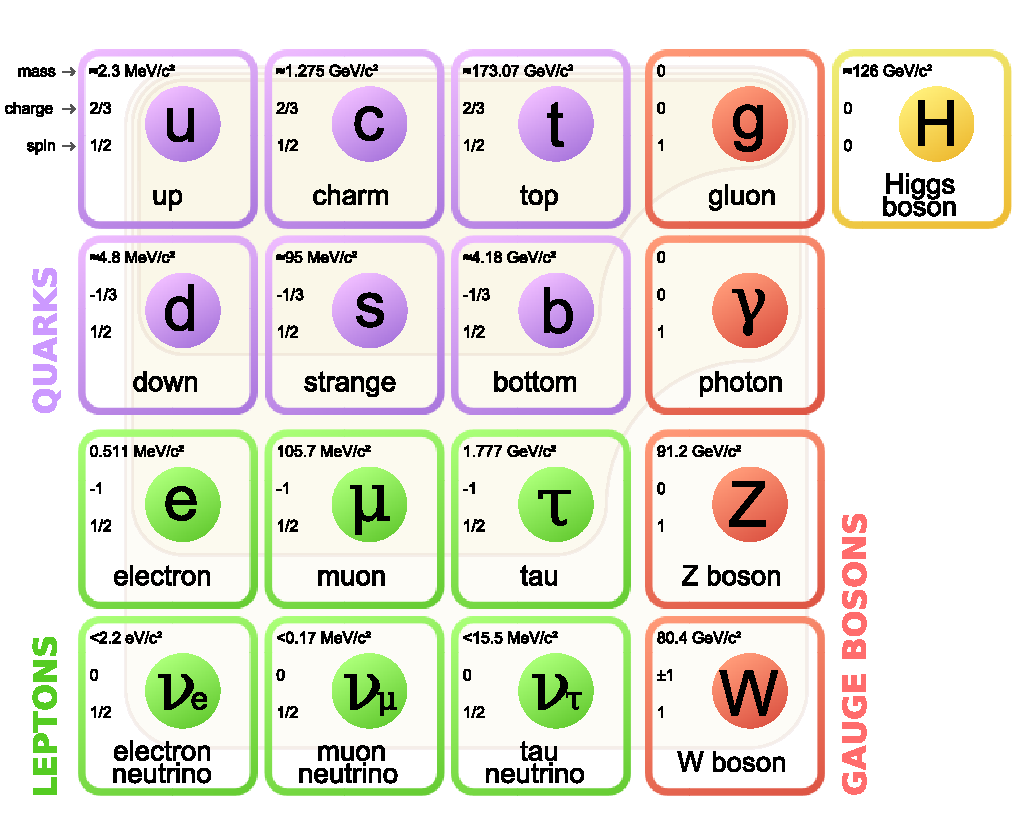
\includegraphics[width=0.7\textwidth]{figs/theory/standardmodel.pdf}
\caption{\label{fig:standardmodel} The particles in the standard model.}
\end{figure}

\begin{table}
\centering
\begin{tabular}{c|ccc}
&$\mathrm{SU(3)}_{\mathrm{C}}$&$\mathrm{SU(2)}_{\mathrm{L}}$&$\mathrm{U(1)}_Y$ \\\hline
$q$ & $\mathbf{3}$ & $\mathbf{2}$ & $1/6$\\
$\bar u_R$ & $\mathbf{\bar 3}$ & $\mathbf{1}$ & $-2/3$\\
$\bar d_R$ & $\mathbf{\bar 3}$ & $\mathbf{1}$ & $1/3$\\
$\ell$ & $\mathbf{1}$ & $\mathbf{2}$ & $-1/2$\\
$\bar e_R$ & $\mathbf{1}$ & $\mathbf{1}$ & $1$\\\hline
$h$ & $\mathbf{1}$ & $\mathbf{2}$ & $1/2$
\end{tabular}
\caption{\label{tab:representations} Table summarizing the
    representations in which the matter fields transform under the standard
    model gauge group. $\mathbf{n}$ ($\mathbf{\bar n}$) is the
    fundamental (antifundamental) representation
    of $\mathrm{SU(n)}$. For the $\mathrm{U(1)}_Y$ factor, the
    representations are labeled by the weak hypercharge $Y$. The electric charge is given by $Q = T_{3L}+Y$. }
\end{table}


\section{Electroweak Symmetry Breaking}
\label{sec:ewsb}
A central feature of gauge theories is that the gauge bosons are
massless due to the fact that the gauge symmetry forbids explicit mass
terms in the Lagrangian. In 1964, it was proposed that
\emph{spontaneous symmetry breaking} could be achieved in gauge
theories through the introduction of a scalar
field~\cite{PhysRevLett.13.321,HIGGS1964132,PhysRevLett.13.508,PhysRevLett.13.585,PhysRev.145.1156,PhysRev.155.1554}. Spontaneous
symmetry breaking means the equations of the dynamics are exactly symmetric, but they
admit solutions that are not. In the SM, the mechanism of electroweak symmetry breaking
is a framework to keep the structure of gauge symmetry and
interactions at high energy, and still generate the observed masses
of the $\PW^{\pm}$ and $\PZ$ gauge
bosons~\cite{PhysRevLett.19.1264,GLASHOW1961579,Salam:1968rm}. 

The part of the Lagrangian that accomplishes this is: 
\begin{align}
\mathcal L_{\mathrm{Higgs}} &= (D_{\mu}\Phi)^{\dagger}(D^{\mu}\Phi) -
V(\Phi)~;& V(\Phi) &= -\mu^2\Phi^{\dagger}\Phi +
\lambda(\Phi^{\dagger}\Phi)^2~,
\label{eqn:Lhiggs}
\end{align}
where the field $\Phi$ is a complex, spin-$0$, self-interacting
$\mathrm{SU(2)}_{\mathrm{L}}$ doublet with weak hypercharge $Y=1/2$:
\begin{equation}
\Phi = \left(\begin{matrix} \phi^{+}\\\phi^0\end{matrix} \right)~.
\end{equation}
If $\mu^2>0$, then the potential will have a ``Mexican hat'' shape, illustrated in
\ref{fig:mexicanhat}, and the minimum of the potential will occur at a value of the field that is not $\mathrm{SU(2)}_{\mathrm{L}}\times\mathrm{U(1)}_Y$
invariant. Due to this, $\Phi$ acquires a nonzero vacuum
expectation value (\emph{vev}), corresponding to the minimum of the potential,
\begin{align}
\langle\Phi\rangle_0&\equiv \langle 0|\Phi|0\rangle =
\frac{1}{\sqrt{2}}U(x)\left(\begin{matrix} 0\\v\end{matrix} \right)~;&v &= \sqrt{\frac{\mu^2}{\lambda}};
\end{align}
where $U(x)$ is a unitary transformation that rotates the field
to the other degenerate solutions. Since the vev is still symmetric under a $\mathrm{U(1)}$ subgroup of the full
electroweak symmetry, we say the electroweak symmetry
$\mathrm{SU(2)}_{\mathrm{L}}\times\mathrm{U(1)}_Y$ is \emph{spontaneously
broken} to $\mathrm{U(1)}_{\mathrm{EM}}$. 

\begin{figure}
\centering
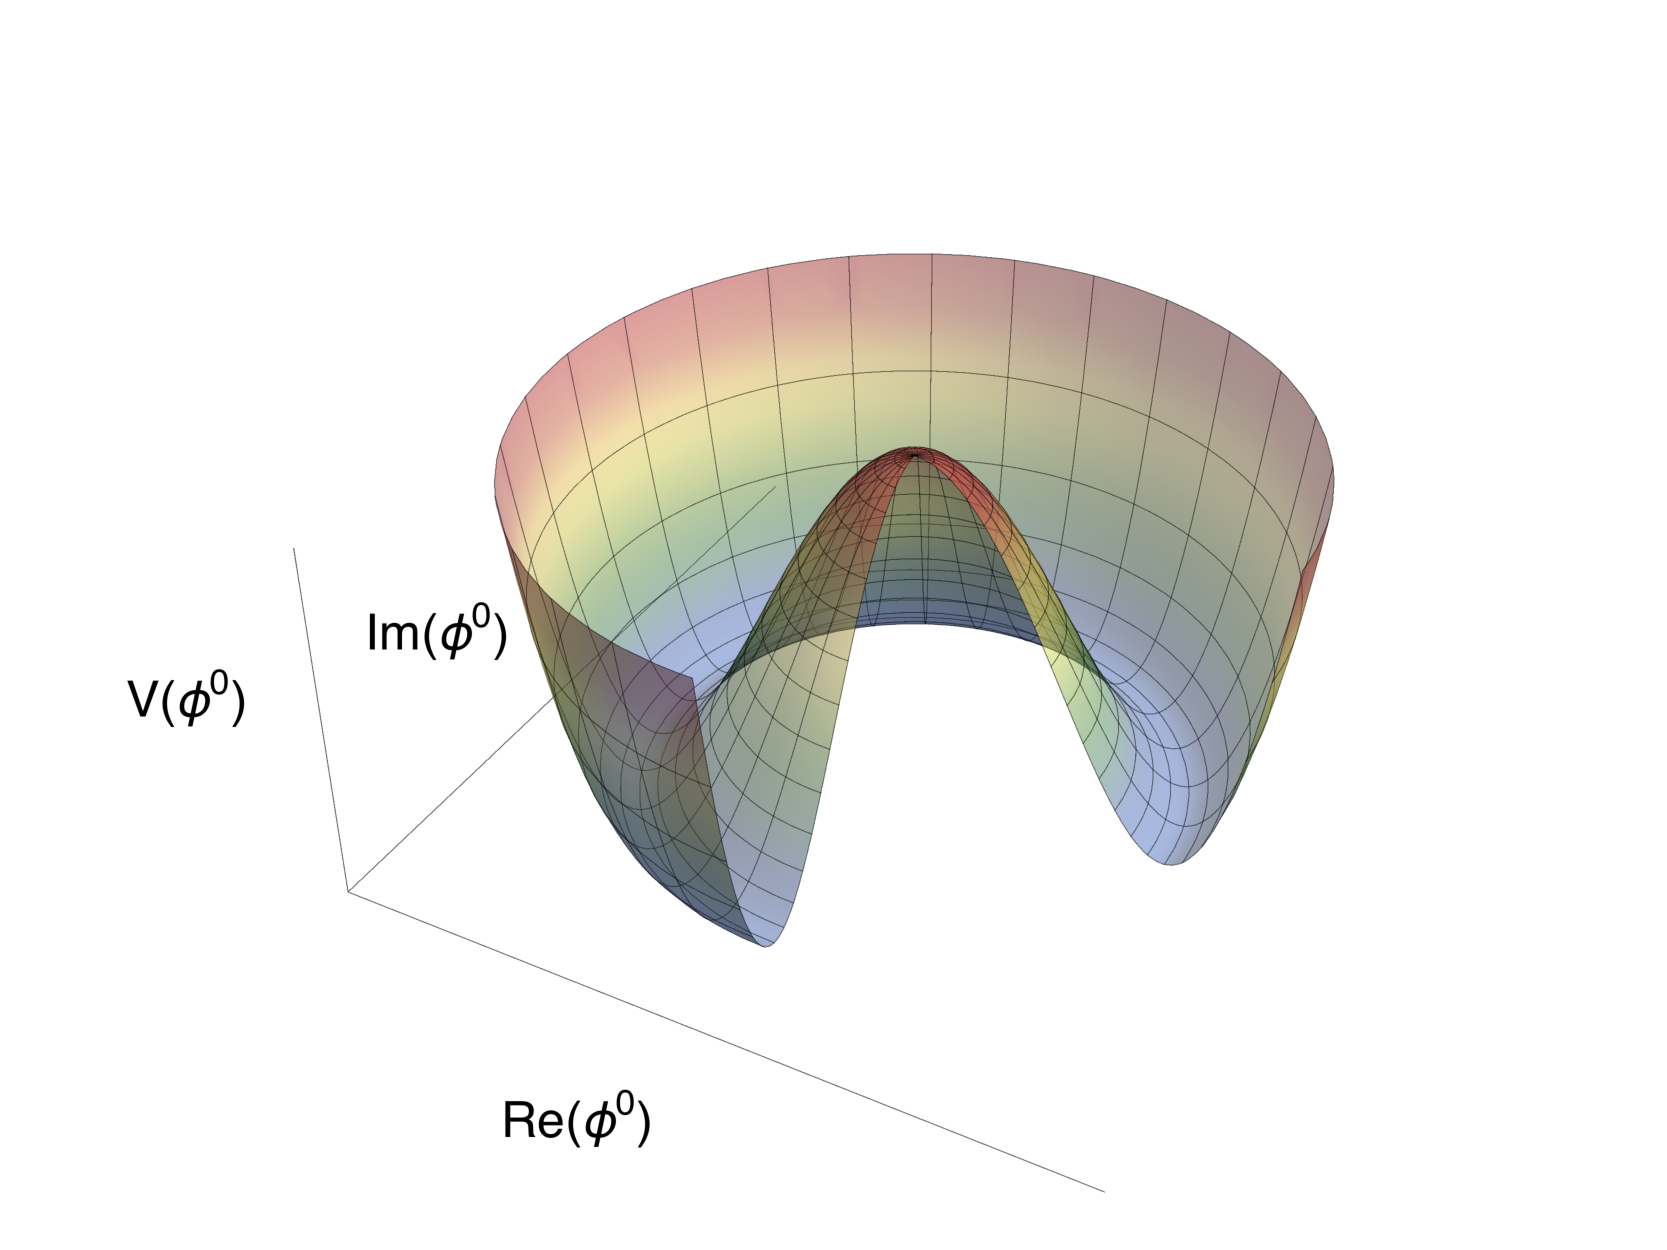
\includegraphics[width=0.7\textwidth]{figs/theory/MexicanHat.pdf}
\caption{\label{fig:mexicanhat} The shape of the ``Mexican hat''
  potential. The minimum of the potential occurs at
a field value that is not $0$.}
\end{figure}

This mechanism is responsible for generating the masses of the gauge
bosons in the standard model, as can be seen by evaluating the 
covariant derivative in Eqn.~\ref{eqn:Lhiggs},
\begin{equation}
D_{\mu}\Phi = (\partial_{\mu} - i g_2 \frac{\sigma_a}{2}W^a_{\mu} -
ig_1\frac{1}{2}B_{\mu})\Phi ~,
\end{equation}
on the vacuum Higgs field. In this case, the kinetic term is:
\begin{align}
|D_{\mu}\Phi|^2 &= \frac{1}{2} \left|\left (\begin{matrix}\partial_{\mu}
    -\frac{i}{2}(g_2W_{\mu}^3 + g_1B_{\mu})&
    -\frac{ig_2}{2}(W_{\mu}^1-iW_{\mu}^2)\\ 
-\frac{ig_2}{2}(W_{\mu}^1+iW^2_{\mu})&\partial_{\mu}
    +\frac{i}{2}(g_2W_{\mu}^3 - g_1B_{\mu})
  \end{matrix}\right)
                                       \left(\begin{matrix}0\\v\end{matrix}\right)\right |^2 \nonumber\\
& = \frac{1}{8} \left ( g_2^2v^2|W_{\mu}^1+iW^2_{\mu}|^2 +
  v^2|g_2W^3_{\mu}-g_1B_{\mu}|^2 \right ) \nonumber\\
& = m_W^2W_{\mu}^+W^{-\mu} +
\frac{1}{2}m_Z^2Z_{\mu}Z^{\mu}~ + \frac{1}{2}m_{\gamma}^2A_{\mu}A^{\mu},
\end{align}
where we can identify three field combinations, $W_{\mu}^{\pm}$ and
$Z_{\mu}$, which have bilinear mass terms, and a fourth $A_{\mu}$,
which does not:
\begin{align}
W_{\mu}^{\pm} &= \frac{1}{\sqrt{2}}(W_{\mu}^1\mp iW^2_{\mu})~, &m_W &= \frac{1}{2}vg_2~,\\
Z_{\mu} &= \frac{g_2W_{\mu}^3 - g_1B_{\mu}}{\sqrt{g_1^2+g_2^2}}~,&m_Z &= \frac{1}{2}v\sqrt{g_1^2+g_1^2}~,\\
A_{\mu} &= \frac{g_2W_{\mu}^3 + g_1B_{\mu}}{\sqrt{g_1^2+g_2^2}}~,&m_{\gamma} &= 0.
\end{align}
The $\PW^{\pm}$ and $\PZ$ bosons have acquired mass, while the photon
$\Pgg$ remains massless.

Another consequence of this symmetry breaking mechanism is the
emergence of a physical spin-$0$ boson. If we expand the field around
its potential minimum
\begin{align}
\Phi(x)&=
\frac{1}{\sqrt{2}}U(x)\left(\begin{matrix} 0\\v+H(x)\end{matrix} \right)
\end{align}
and write out the terms associated to this field, we find
\begin{equation}
\mathcal L_{\mathrm{Higgs}} \supset \frac{1}{2}(\partial^{\mu}H)^2 -
\lambda v^2 H^2 - \lambda v H^3 - \frac{\lambda}{4}H^4~.
\end{equation}
which means this scalar boson, called the \emph{Higgs boson}, is self-interacting and has a mass squared of $m^2_{h^0} =
2\lambda v^2$ at tree-level.

\section{Fermion Masses}
\label{sec:fermionmasses}
As proposed by Weinberg~\cite{PhysRevLett.19.1264}, fermions acquire
mass through interaction with the $\Phi$ field, which has a nonzero
vev. This is accomplished by adding Yukawa terms to the Lagrangian for
each generation,
\begin{equation}
\mathcal L_{\mathrm{Yukawa}} = - y_e \bar\ell_L\Phi e_R -
y_u\bar q_L\Phi u_R  - y_d\bar q_L\tilde\Phi d_R + (\mathrm{h.c.})~,
\end{equation}
where the doublet $\tilde\Phi = i\sigma_2\Phi^{\ast}$ with hypercharge $Y=-1/2$ is
needed to generate masses for the down-type quarks. Then we can
identify the fermion masses as
\begin{align}
m_e &= \frac{y_e v}{2}&m_u &= \frac{y_u
                                          v}{2}& m_d &= \frac{y_dv}{2}~.
\end{align}
%Neutrino masses can also be accommodated in the SM by adding similar
%terms. 
Besides giving masses to the fermions, the Yukawa terms have another important
consequence: they allow the fermions to affect the
observed mass of the Higgs boson through quantum corrections.

\chapter{Naturalness and Supersymmetry}
\label{ch:naturalness}
\section{Naturalness in the Standard Model}
\label{sec:higgsnaturalness}
The leading quantum correction to the Higgs mass is due to
the large Yukawa coupling of the top quark, which gives the
top quark its large mass. In an effective field theory approach, where
momenta of virtual particles are cut off at the scale
$\Lambda_{\mathrm{UV}}$, we can compute the top quark's contribution in the SM to leading order,
\begin{fmffile}{higgs}
\begin{align}
m^2_{h^0} &= m^2_{h^0\mathrm{(bare)}} +\Delta(m^2_{h^0}) \\
\Delta(m^2_{h^0}) &= \quad\parbox{20mm}{
\begin{fmfgraph*}(20,20)
\fmfkeep{fermion}
\fmfleft{i} 
\fmfright{o} 
\fmf{dashes}{i,v1}
\fmf{dashes}{v2,o}
\fmf{plain,left,tension=.3,label=$t$}{v1,v2}
\fmf{plain,left,tension=.3}{v2,v1}
\fmfv{label=$h^0$,label.angle=90}{i}
\end{fmfgraph*}} \quad + \quad\cdots\\
&= -\frac{3|y_t|^2}{8\pi^2}\Lambda_{\mathrm{UV}}^2 + \cdots~,
\label{eqn:toploop}
\end{align}
The quadratic dependence in Eqn.~\ref{eqn:toploop} on
$\Lambda_{\mathrm{UV}}$, usually taken to be the Planck scale $10^{19}
\GeV$, means the Higgs mass is sensitive to new physics in the
ultraviolet. Taken literally, this sensitivity implies an enormous fine tuning of
$m^2_{h^0\mathrm{(bare)}}$ to achieve almost perfect
cancellation\footnote{to $1$ part in $10^{34}$} with
$\Delta(m^2_{h^0})$ in order to explain how $m_{h^0}$
is measured to be so small at $125.09\pm0.24 \GeV$~\cite{Aad:2015zhl}. The conundrum of how a light fundamental
scalar particle can exist in the presence of (presumably) new physics
in the ultraviolet is called the \emph{naturalness problem} and is one
of the key motivations for new physics at the \TeV scale, especially \emph{supersymmetry}.


\section{Supersymmetry}
\label{sec:susy}
Supersymmetry (SUSY) is a proposed symmetry of spacetime that 
introduces a bosonic (fermionic) partner for every fermion
(boson)~\cite{Wess,Golfand,Volkov,Chamseddine,Kane,Fayet,Barbieri,Hall,Ramond}. For
many years, such a symmetry was thought to be impossible since in 1967,
Colman and Mandula~\cite{PhysRev.159.1251} published their no-go theorem that says
internal symmetries, those that act on internal degrees of
freedom like spin, cannot be combined with spacetime symmetries in a
nontrivial way. SUSY evades this theorem because it is based
on a \emph{super Lie algebra}, which may include fermionic symmetries
and anticommutation relations as well as the usual bosonic symmetries
and commutation relations.

Supersymmetric extensions of the SM are compelling 
because they 
\begin{enumerate}[(a)]
\item yield a solution to the naturalness problem, alleviating
the fine-tuning of fundamental
parameters~\cite{Witten:1981nf,Dimopoulos:1981zb,Dine:1981za,Dimopoulos:1981au,Sakai:1981gr,Kaul:1981hi},
explained further in Sec.~\ref{sec:susynaturalness}.
\item exhibit gauge coupling
  unification~\cite{Dimopoulos:1981yj,Marciano:1981un,Einhorn:1981sx,Ibanez:1981yh,Amaldi:1991cn,Langacker:1995fk}, and
\item provide a weakly interacting particle candidate for dark matter~\cite{Ellis:1983ew,Jungman:1995df}.
\end{enumerate}

SUSY can be thought of as an extension of the usual group of spacetime
symmetries, known as the Poincar\'{e} group. This group has
generators related to translation symmetry, $P_m$, and Loretnz
symmetry, $M_{mn} = -M_{nm}$, which form a Lie algebra:
\begin{align}
~[P_m,P_n] &= 0 \nonumber\\
~[P_m,M_{np}] &= i(\eta_{mn}P_p-\eta_{mp}P_n) \nonumber\\
~[M_{mm},M_{pq}] &= i(\eta_{mp}M_{np} - \eta_{np}M_{mq} +
                   \eta_{nq}M_{mp} - \eta_{mq}M_{np} )~.
\label{eqn:poincare}
\end{align}

As shown by Coleman and Mandula~\cite{PhysRev.159.1251}, the only way
to extend this symmetry with a new internal symmetry group $G$ with bosonic
generators $B_r$ and Lie algebra,
\begin{equation}
~[B_r,B_s] = f_{rs}{}^tB_t~,
\end{equation}
with structure functions $f_{rs}{}^t$, is if the extended symmetry
group is simply the direct product $($Poincar\'{e}$)\times G$ with a
trivial Lie algerbra,
\begin{equation}
~[B_r,P_m] = [B_r,M_{mn}] = 0~.
\end{equation}

However, SUSY exploits a loophole in the Coleman-Mandula theorem,
which only considers bosonic symmetry generators, by incorpororating
fermionic symmetry generators $Q$ that generate SUSY transformations,
\begin{equation}
Q|\mathrm{boson}\rangle = |\mathrm{fermion}\rangle, ~~~~
Q|\mathrm{fermion}\rangle = |\mathrm{boson}\rangle~.
\end{equation}
Supersymmetries can be combined with the
spacetime symmetries in a way that mixes the two symmetries, as
exemplified by the super Lie algebra for $\mathcal N=1$
SUSY,
\begin{align}
~\{ Q_{\alpha},\bar Q_{\dot{\beta}}\} &= 2\sigma^m_{\alpha\dot\beta} P_m \nonumber\\
~\{ Q_{\alpha},Q_{\beta}\} &= \{ \bar Q_{\dot\alpha},\bar Q_{\dot\beta}\} = 0\nonumber\\
~[ P_m, Q_{\alpha}] &= [P_m,\bar Q_{\dot\alpha}] = 0~.
\label{eqn:n1susy}
\end{align}
In other words, two SUSY generators can combine to generate a spacetime translation.

The most economical supersymmetric extension of the standard model is the
Minimal Supersymmetric Standard Model (MSSM). For supersymmetric
theories, the Lagrangian can be written in terms of vector superfields
$V(x,\theta,\bar\theta)$ and chiral superfields $\Phi_l(x,\theta,\bar\theta)$ that are functions of
\emph{superspace}, an extension of spacetime that includes
anticommuting Grassmanian variables $\theta$ and
$\bar\theta$. Tab~\ref{tab:susyreps} shows the particles of the
MSSM, described by chiral superfields $Q_i, U_i^c, L_i, E_i^c, H_u,
H_d$, and the representations in which they transform under the MSSM gauge group.
\begin{table}
\centering
\begin{tabular}{c|ccc}
&$\mathrm{SU(3)}_{\mathrm{C}}$&$\mathrm{SU(2)}_{\mathrm{L}}$&$\mathrm{U(1)}_Y$ \\\hline
$Q$ & $\mathbf{3}$ & $\mathbf{2}$ & $1/6$\\
$U^c$ & $\mathbf{\bar 3}$ & $\mathbf{1}$ & $-2/3$\\
$D^c$ & $\mathbf{\bar 3}$ & $\mathbf{1}$ & $1/3$\\
$L$ & $\mathbf{1}$ & $\mathbf{2}$ & $-1/2$\\
$E^c$ & $\mathbf{1}$ & $\mathbf{1}$ & $1$\\\hline
$H_u$ & $\mathbf{1}$ & $\mathbf{2}$ & $1/2$\\
$H_d$ & $\mathbf{1}$ & $\mathbf{2}$ & $-1/2$
\end{tabular}
\caption{\label{tab:susyreps} Table summarizing the
    representations in which the chiral superfields transform under
    the MSSM gauge group. See Tab.~\ref{tab:representations} for a
    description of the columns.}
\end{table} 

The MSSM Lagrangian can be split into three terms, the K\"{a}hler potential $K(\Phi_l,\Phi_l^{\dagger},V)$,
which describes the kinetic and gauge-covariant terms, a superpotential $W(\Phi_l)$, which
describes the mass and interaction terms, and a gauge kinetic term $G(V)$,
\begin{align}
\mathcal L_{\mathrm{MSSM}} &= \int \mathrm{d}^4\theta
K(\Phi_l,\Phi_l^{\dagger},V) + \left (\int
 \mathrm{d}^2\theta W(\Phi_l) + \mathrm{h.c.} \right) + \left (\int
\mathrm{d}^2\theta G(V) +
\mathrm{h.c.}\right )\nonumber\\
&= \int \mathrm{d}^4\theta
\sum_{V}
\Phi_{l}^{\dagger}e^{gV}\Phi_{l} + \left (\int
 \mathrm{d}^2\theta W(\Phi_l) + \mathrm{h.c.} \right) + \left (\int
\mathrm{d}^2\theta \frac{1}{4}\mathcal W^{\alpha}\mathcal W_{\alpha} +
\mathrm{h.c.}\right )~,
\label{eqn:mssmlag}
\end{align}
where $\mathcal W_{\alpha}$ is the vector superfield strength\footnote{The vector superfield strength is $\mathcal W_{\alpha} =
  -\frac{1}{4} \bar{\mathcal{D}}^2(e^{-V}\mathcal{D}_{\alpha}
  e^{V})$.} and the index $l$ runs over all the matter superfields
$\Phi_l = Q_i, U_i^c, L_i, E_i^c, H_u, H_d$. The superpotential can be
split into two components based on $R$-parity, a discrete $Z_2$
symmetry often assumed in SUSY model building, defined for each
particle as 
\begin{equation}
P_R = (-1)^{(\mathrm{B}-\mathrm{L})+2s}
\end{equation}
where $\mathrm{B}$ is the baryon number, $\mathrm{L}$ is the lepton number, and $s$ is the spin
of the particle. With this assignment, all SM particles have even
$R$-parity ($P_R=+1$), while the superpartners have odd $R$-parity
($P_R=-1$). The $R$-parity conserving terms in the superpotential are
\begin{equation}
W_{\mathrm{RPC}} = - U^c\mathbf{y_u} Q H_u + D^c\mathbf{y_d}QH_d  +
E^c\mathbf{y_e} L H_d +
\mu H_uH_d~,
\label{eqn:Wrpc}
\end{equation}
and the $R$-parity violating terms are
\begin{equation}
W_{\mathrm{RPV}} =\frac{1}{2}\lambda^{ijk}L_iL_jE_k^c +
\lambda^{\prime ijk} L_iQ_jD_k^c + \mu^{\prime i}H_uL_i +
\frac{1}{2}\lambda^{\prime\prime ijk}U_i^cD_j^cD_k^c~.
\label{eqn:Wrpv}
\end{equation}

If $R$-parity is conserved, there are three important phenomenological consequences:
\begin{itemize}
\item The lightest superparter, called the ``lightest
  supersymmetric particle'' or LSP, must be stable. 
\item Each superpartner other than the LSP must eventually decay into a
  state that contains an odd number of LSPs (usually just one).
\item In collider experiments, superpartners can only be produced in even numbers (usually two).
\end{itemize}

\textbf{NEED TO DISCUSS SOFT SUSY BREAKING}

\section{Elecroweak Supersymmetric Sector}
\label{sec:ewksusy}
The superpartners of the neutral gauge bosons (neutral gauginos), and
the fermionic partners of the neutral Higgs bosons (neutral higgsinos),
$\psi^0 =(\PSB,\PSWz,\PSHdz,\PSHuz)$, mix to form the
\emph{neutralinos} $(\chiz_1, \chiz_2, \chiz_3, \chiz_4)$. Similarly, the superpartners of the charged gauge bosons
(charged gauginos) and the fermionic partners of the charged Higgs
bosons (charged higgsinos), $\psi^{\pm}=(\PSWp,\PSHup,\PSWm, \PSHdm)$ mix to form the charginos
$(\chip_1, \chip_2, \chim_1, \chim_2)$. In this gauge-eigenstate basis, the neutralino
and chargino mass terms in the Lagrangian are
\begin{equation}
\mathcal L_{\mathrm{MSSM}} \supset -\frac{1}{2}\psi^{0T}\mathbf{M}_N \psi^0 -\frac{1}{2}\psi^{\pm T}\mathbf{M}_C \psi^{\pm} + \mathrm{h.c.}
\end{equation}
with the neutralino mass matrix,
\begin{equation}
\mathbf{M}_N =\left (  \begin{matrix}
M_1 & 0 & -m_Zs_Wc_{\beta} & m_Zs_Ws_{\beta} \\
0& M_2 & -m_Zc_Wc_{\beta} & -m_Zc_Ws_{\beta} \\
-m_Zs_Wc_{\beta}& m_zc_Wc_{\beta} & 0 & -\mu\\
m_Zs_Ws_{\beta}& -m_zc_Ws_{\beta} & \mu & 0
\end{matrix}\right)~,
\end{equation}
and the chargino mass matrix,
\begin{equation}
\mathbf{M}_C =\left (  \begin{matrix}
0 & \mathbf{X}^T \\
 \mathbf{X}& 0
\end{matrix}\right), ~\mathrm{where} ~ \mathbf{X} = \left (  \begin{matrix}
M_2 & \sqrt{2}m_Ws_{\beta}\\
 \sqrt{2}m_Wc_{\beta}& \mu
\end{matrix}\right)~,
\end{equation}
where $M_2$ and $M_1$ are the wino and bino mass terms, respectively.
The eigenvalues of these matrices are the masses of the
neutralinos and charginos.

\section{Naturalness in Supersymmetry}
\label{sec:susynaturalness}

For SUSY to provide a ``natural'' solution to the gauge hierarchy problem,
the top squark, bottom squark, and gluino must have masses below a few
TeV, making them accessible at the CERN LHC. To make this statement
quantitative, we first need to define a measure of
fine-tuning, such as~\cite{Brust:2011tb,naturalSUSY}:
\begin{equation}
\Delta = \frac{\Delta(m^2_{h^0})}{m^2_{h^0}}~.
\end{equation}
%Other measures of fine-tuning are possible, such as those in...

In the decoupling limit of the MSSM at tree-level, the mass of the
physical Higgs boson satisfies
\begin{equation}
m^2_{h^0} = -2(m_{H_u}^2 + |\mu|^2) =  m_Z^2\cos^2(2\beta)  ~.
\end{equation}
Due to this tree-level relation between $\mu$, which controls the
masses of the higgsinos, and $m^2_{h^0}$, we expect both $\mu$ to be
small and the higgsinos to be light in order to keep $m^2_{h^0}$
small. When $\mu$ is small ($\mu \ll M_1, M_2$), the two lightest
neutralinos and the lightest chargino are higgsino-like and their
masses are close together~\cite{PhysRevD.37.2515},
\begin{align}
m_{\chiz_1} &= |\mu| + \frac{m_Z^2(1+s_{\beta})(\mu - M_1c_W^2-M_2s_W^2)}{2(\mu-M_1)(\mu-M_2)} + \cdots\\
m_{\chiz_2} &= |\mu| + \frac{m_Z^2(1-s_{\beta})(\mu + M_1c_W^2+M_2s_W^2)}{2(\mu+M_1)(\mu+M_2)} + \cdots\\
m_{\chipm_1} &= |\mu| - \frac{m_W^2(\mu + M_2\sin 2\beta)}{M_2^2-\mu^2} + \cdots~.
\end{align}
Fig.~\ref{fig:neutralinos} shows the mass differences
$m_{\chipm_1}-m_{\chiz_1}$ and $m_{\chiz_2}-m_{\chiz_1}$ as a function of the wino mass $M_2$.

\begin{figure}[tb!]
\centering
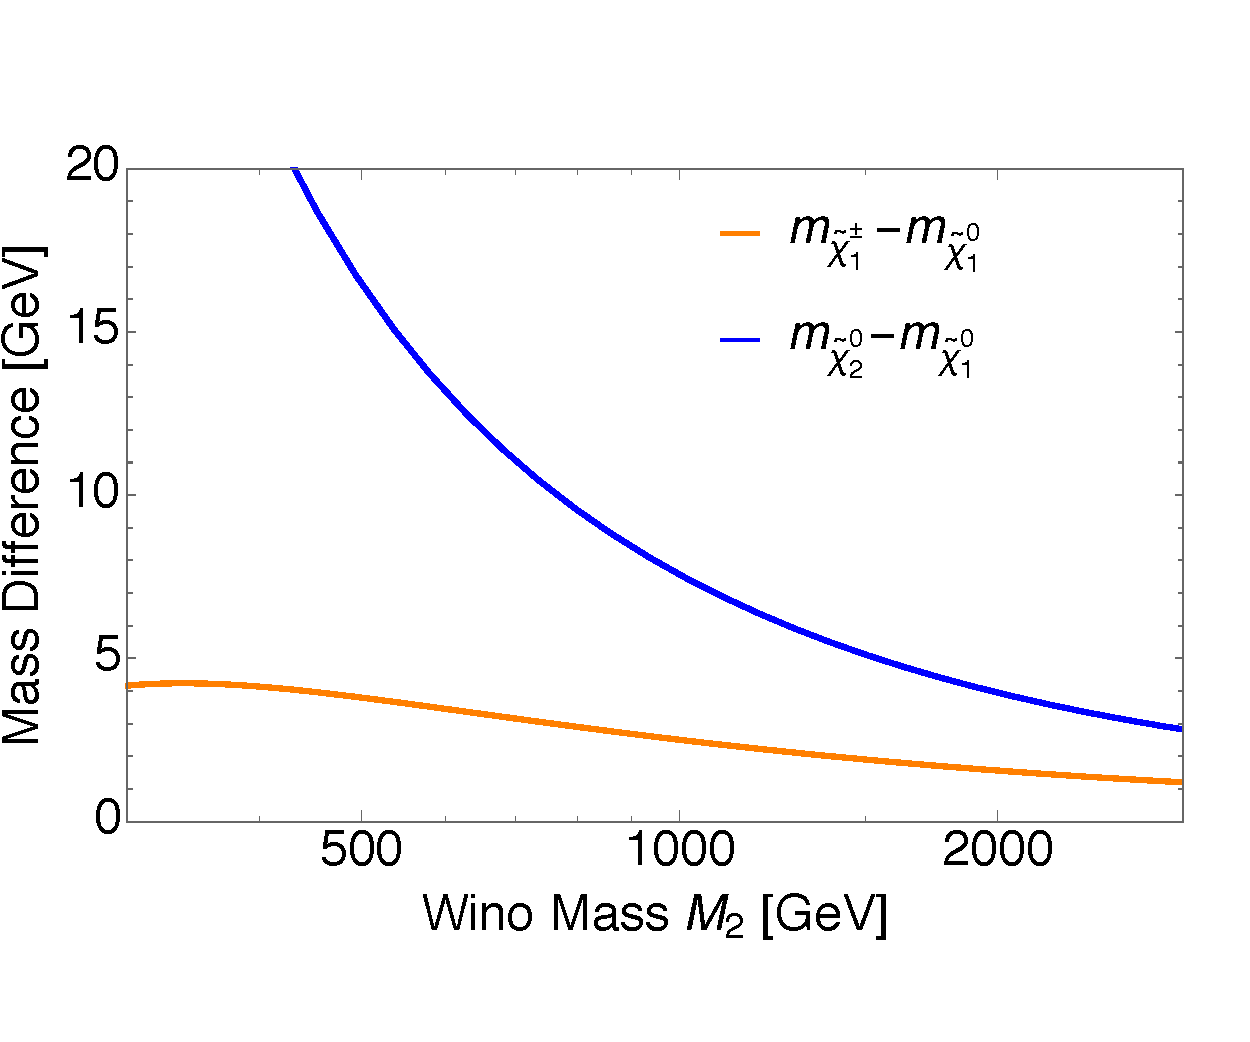
\includegraphics[width=0.8\textwidth,clip=true,viewport= 0 30 610 450]{figs/theory/neutralinos.pdf}
\caption{The mass difference between the lightest chargino and the
  lightest neutralino as a function of the wino mass $M_2$
  assuming $\tan\beta=10$, $\mu=200 \GeV$ and $M_1 = 3 \TeV$.\label{fig:neutralinos}}
\end{figure}

There are additional considerations at loop level. In particular the
top squark has a large radiative correction which partially cancels
with the contribution from the top quark in Eqn.~\ref{eqn:toploop}:
\begin{align}
\Delta(m^2_{h^0}) &= \quad\parbox{20mm}{\fmfreuse{fermion}} \quad + \quad
\parbox{20mm}{
\begin{fmfgraph*}(20,20)
\fmfkeep{boson}
\fmfleft{i} 
\fmfright{o} 
\fmf{dashes}{i,v}
\fmf{dashes,right,tension=0.7,label=$\tilde t_{1,,2}$}{v,v}
\fmf{dashes}{v,o}
\fmfv{label=$h^0$,label.angle=90}{i}
\end{fmfgraph*}}
 \quad + \quad
\parbox{20mm}{
\begin{fmfgraph*}(20,20)
\fmfkeep{sunset}
\fmfleft{i}
\fmfright{o}
\fmf{dashes}{i,v1}
\fmf{dashes}{v2,o}
\fmf{dashes,left,tension=.3,label=$\tilde t_{1,,2}$}{v1,v2}
\fmf{dashes,left,tension=.3}{v2,v1}
\fmfv{label=$h^0$,label.angle=90}{i}
\end{fmfgraph*}} \quad + \quad\cdots\\
 &= -\frac{3|y_t|^2}{8\pi^2}\Lambda_{\mathrm{UV}}^2 +
  \sum_{i=1}^{2} \left ( \frac{3|y_t|^2}{16\pi^2}\Lambda_{\mathrm{UV}}^2 - \frac{3|y_t|^2m_{\tilde
  t_i}^2}{8\pi^2}\log\left (\frac{\Lambda_{\mathrm{UV}}}{m_{\tilde
   t_i}}\right ) \right )+ \cdots \\
 &= -\sum_{i=1}^{2} \left ( \frac{3|y_t|^2m_{\tilde
  t_i}^2}{8\pi^2}\log\left (\frac{\Lambda_{\mathrm{UV}}}{m_{\tilde
   t_i}}\right ) \right )+ \cdots~,
\label{eqn:stoploop}
\end{align}
The cancellation of the term proportional to $\Lambda_{\mathrm{UV}}^2$
in Eqn.~\ref{eqn:stoploop} is one of the major successes of SUSY as a candidate for physics beyond
the SM. The sensitivity of the Higgs mass to ultraviolet new
physics is now logarithmic instead of quadratic. If SUSY were an exact
symmetry (and $m_t=m_{\tilde t_{1,2}}$) then the cancellation would be
exact and there would be no further naturalness problem. As it stands, however, we know SUSY is broken, and the
remaining term may also be large depending on the difference in masses
between the top quark and top squarks. Therefore, naturalness places constraints on the allowed masses of the top
squarks given an ``acceptable'' level of fine tuning.

Very roughly, naturalness requires $m_{\tilde t_{i}}\lesssim
400 \GeV$ if $\Lambda_{\mathrm{UV}}\approx
10\TeV$ implying a fine tuning of the order of
10\%~\cite{Brust:2011tb,Craig:2013cxa}. 
%A more complete treatment takes into
%account top squark mixing~\cite{Kitano:2006gv,naturalSUSY},
%\begin{equation}
%\Delta(m^2_{h^0}) = \frac{3|y_t|^2}{4\pi^2}\left ( m_{Q_3}^2 + m_{U_3}^2 + |A_t|^2 \right ) \log\left(
 % \frac{\Lambda_{\mathrm{mess}}}{m_{\tilde t}} \right)
%\end{equation}

There is also a two-loop contribution to the Higgs mass parameter from
the gluino, which is closely related to the one-loop contribution to
the stop mass from the gluino
\begin{align}
\Delta(m^2_{\tilde t_i}) &= \quad 
\parbox{20mm}{
\begin{fmfgraph*}(20,20)
\fmfkeep{gluinosunset}
\fmfleft{i}
\fmfright{o}
\fmf{dashes}{i,v1}
\fmf{dashes}{v2,o}
\fmf{gluon,left,tension=.3,label=$\tilde g$}{v1,v2}
\fmf{plain,left,tension=.3,label=$t$}{v2,v1}
\fmfv{label=$\tilde t_{i}$,label.angle=90}{i}
\fmffreeze
\fmf{plain,left,tension=.3}{v1,v2}
\end{fmfgraph*}} + \quad \cdots\\
&= \frac{2g_s^2m_{\tilde g}^2}{3\pi^2}\log \left
  (\frac{\Lambda_{\mathrm{UV}}}{m_{\tilde g}} \right) + \cdots~,
\end{align}
\end{fmffile}
With this, we have roughly that $m_{\tilde g} \lesssim 2 m_{\tilde t}$.

Taking these relationships at tree, one-loop, and two-loop levels into
consideration, there are three requirements for a minimal natural SUSY spectrum~\cite{naturalSUSY}:
\begin{enumerate}[(a)]
\item quasi-degenerate higgsino-like chargino $\chipm_1$ and two
  neutralinos $\chiz_1, \chiz_2$, below
  $200 - 350 \GeV$, 
\item two stops $\sTop_{1,2}$ and one (left-handed) $\sBot_1$ below
  $500-700 \GeV$, and
\item a gluino below $900 - 1500 \GeV$.
\end{enumerate}

\section{Simplified Natural Supersymmetry Models}
\label{sec:sms}

\begin{figure}[htb!]
\centering
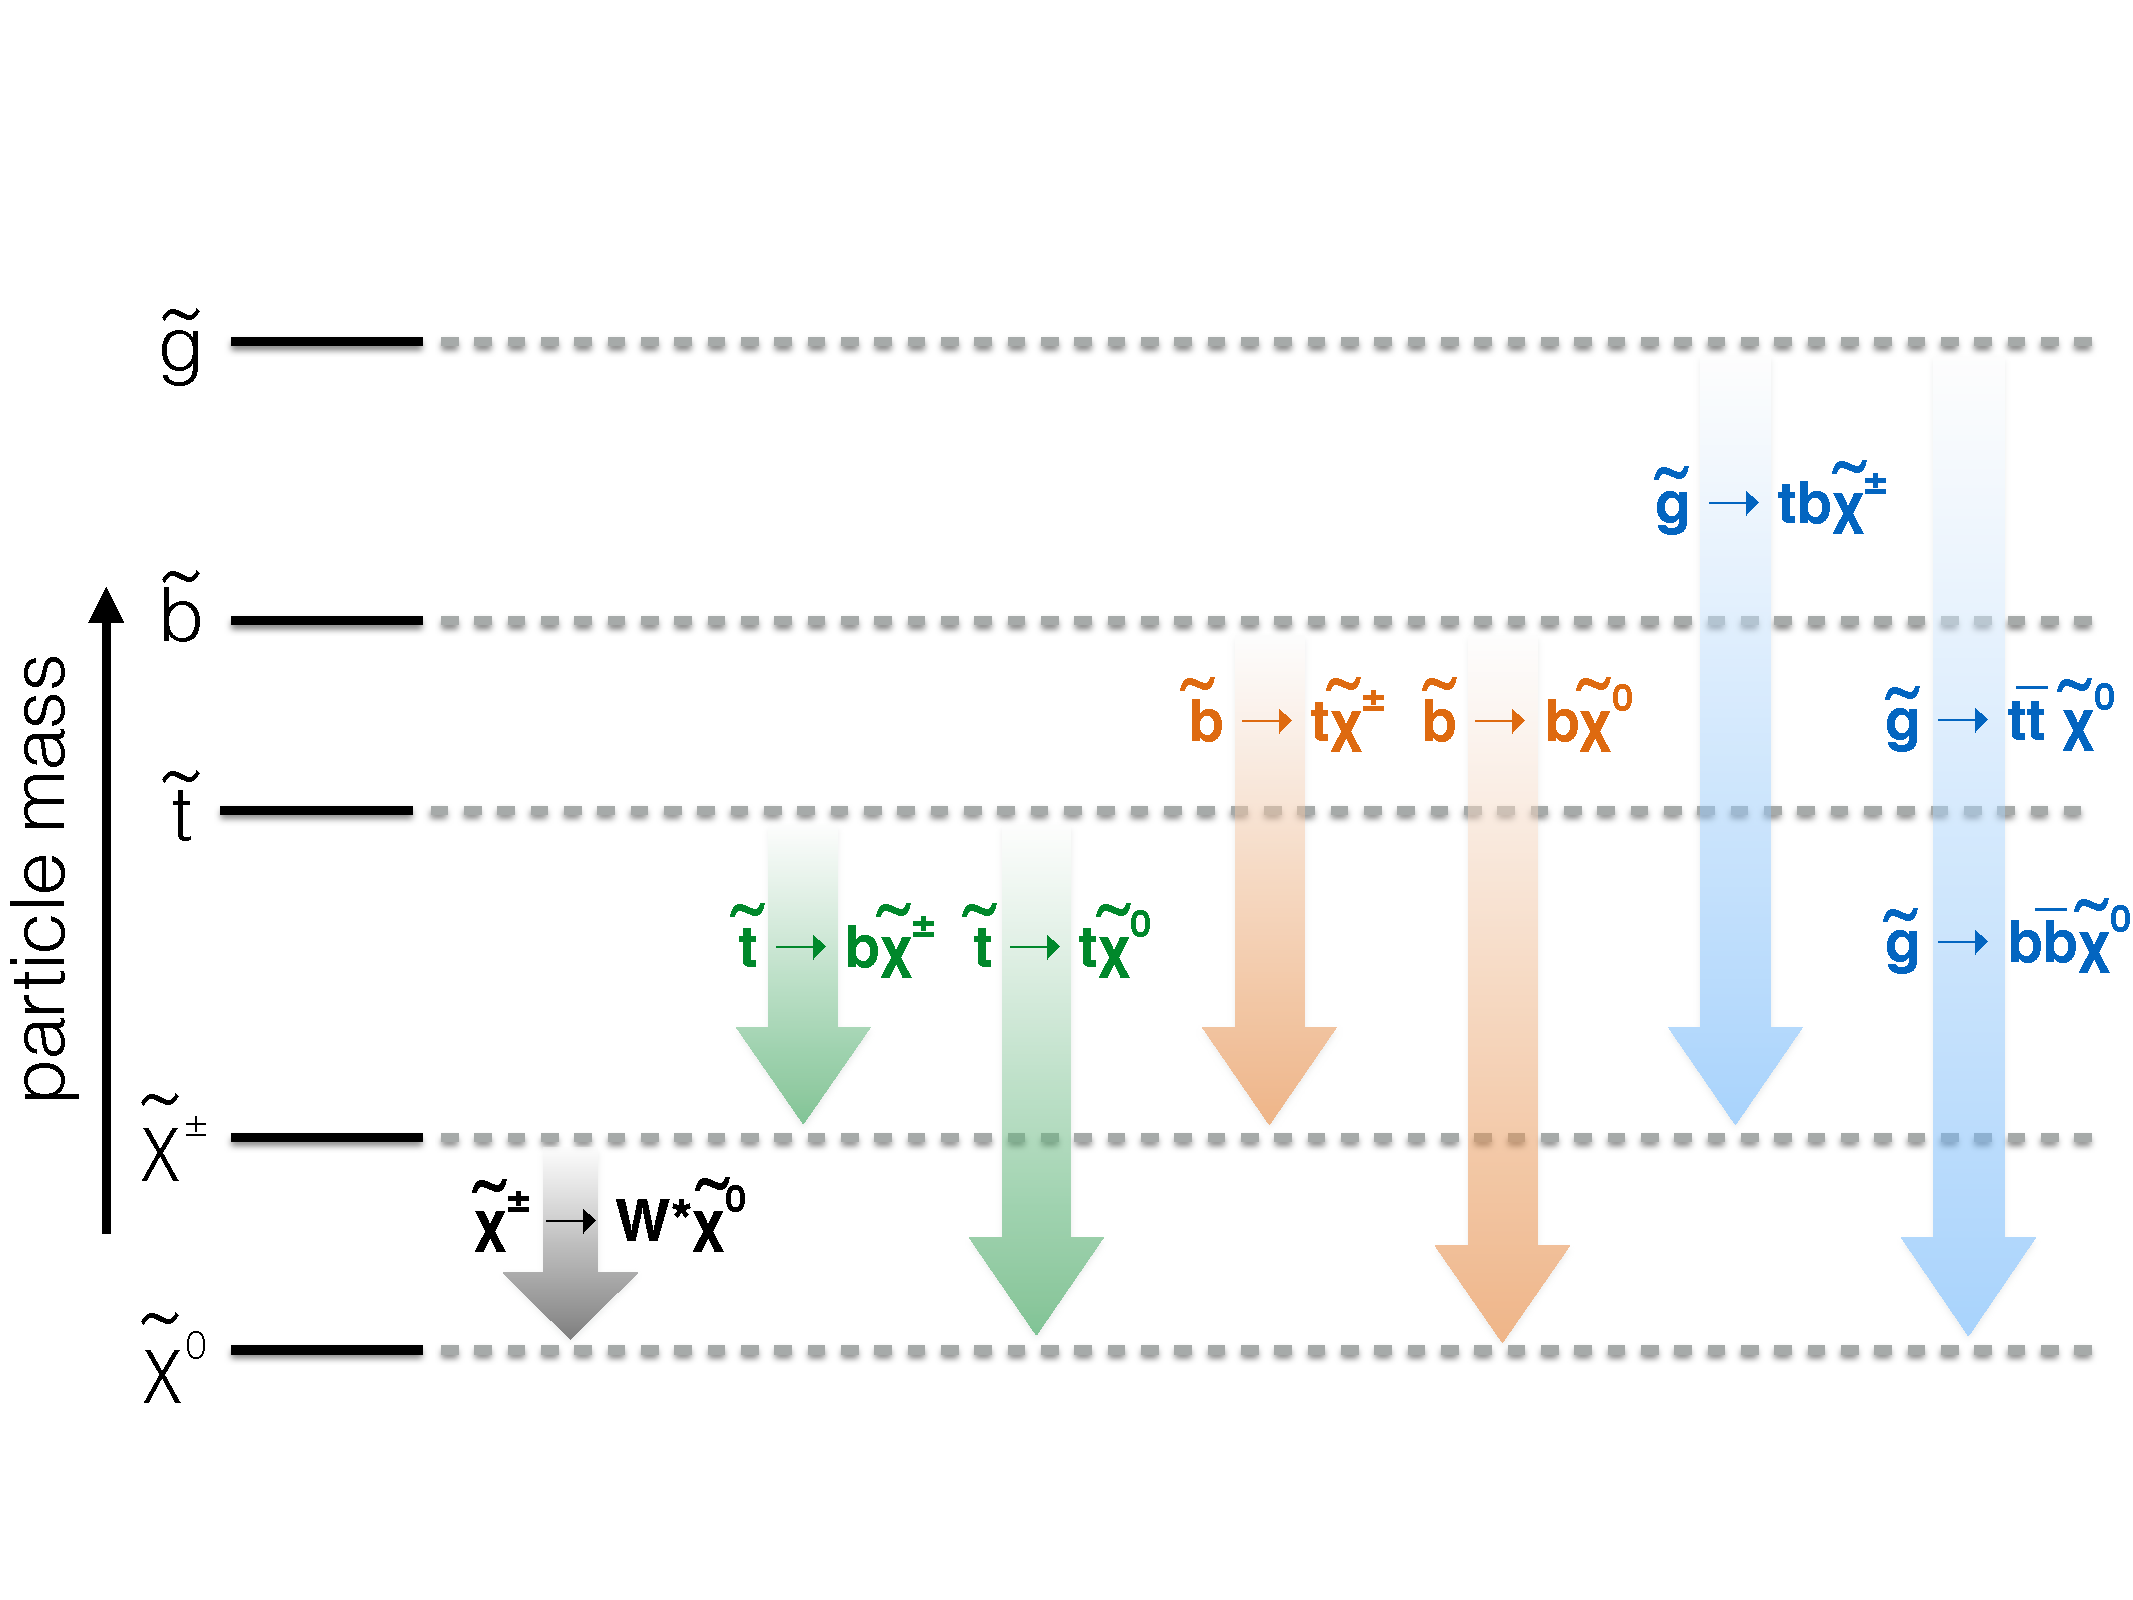
\includegraphics[width=0.85\textwidth]{figs/analysis8TeV/naturalSpectrum.pdf}
\caption{\label{fig:spectrum} The simplified natural SUSY spectrum
  considered in this paper, along with the assumed decay modes.}
\end{figure}

In Ch.~\ref{ch:analysis8TeV} and Ch.~\ref{ch:analysis13TeV}, natural simplified SUSY scenarios are used to interpret
results. The LSP is the lightest neutralino $\chiz_1$ while the NLSP
is the lightest chargino $\chipm_1$.  They are both higgsinos and
their mass splitting is taken to be 5\GeV, motivated by
Fig.~\ref{fig:neutralinos}. The NLSP decays to the LSP and a virtual $\PW$ boson ($\chipm_1 \to \PW^{\ast} \chiz_1$). The
other SUSY particles accessible at the LHC are the gluino and the
lightest top and bottom squarks. All other SUSY particles are
assumed to be too heavy to participate in the interactions. The SUSY
particles and their possible decay modes within this natural SUSY
spectrum are summarized in Fig.~\ref{fig:spectrum}.

In the context of this natural spectrum, several simplified
models~\cite{ArkaniHamed:2007fw,Alwall:2008ag,Alwall:2008va,Alves:2011sq,Alves:2011wf,Graesser:2012qy}
are considered for gluino pair production, based on three-body gluino
decays, in which each gluino decays to one of the following final states~\cite{SUS-11-016}:
\begin{itemize}
\item a top quark (antiquark) and a bottom antiquark (quark),
  and the NLSP; 
\item a top quark-antiquark ($\ttbar$) pair and the LSP;
\item a bottom quark-antiquark ($\bbbar$) pair and the LSP.
\end{itemize}
Furthermore, we separately consider the case in which each gluino
decays to
\begin{itemize}
\item a first or second generation quark-antiquark ($\qqbar$) pair and the LSP.
\end{itemize}

\begin{figure*}[thb!]
\centering
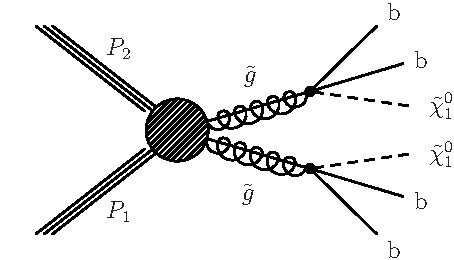
\includegraphics[width=0.32\textwidth]{figs/theory/T1bbbb.pdf}
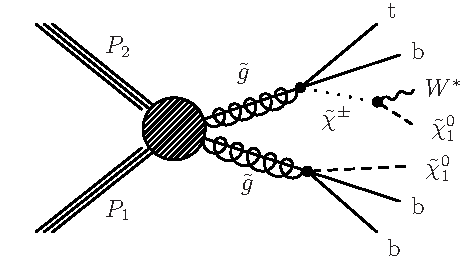
\includegraphics[width=0.32\textwidth]{figs/theory/T1tbbb.pdf}
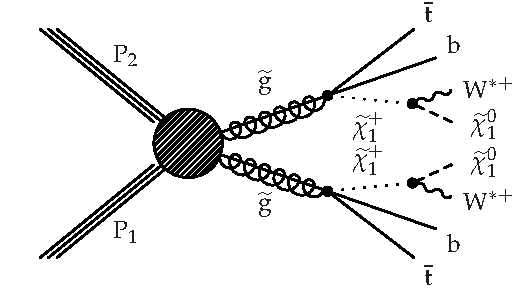
\includegraphics[width=0.32\textwidth]{figs/theory/T1ttbb.pdf} \\
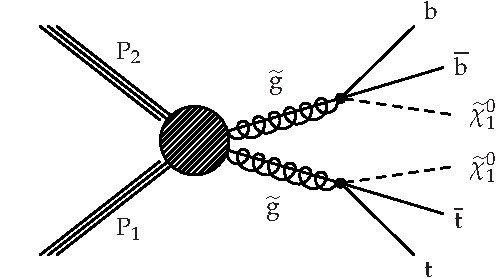
\includegraphics[width=0.32\textwidth]{figs/theory/T1tbtb.pdf} 
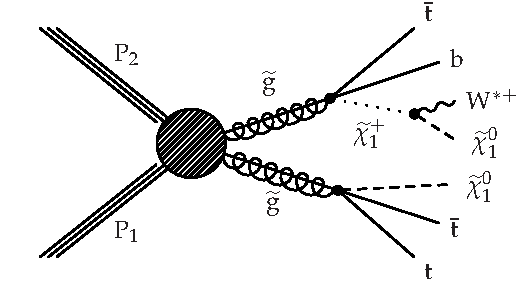
\includegraphics[width=0.32\textwidth]{figs/theory/T1tttb.pdf}
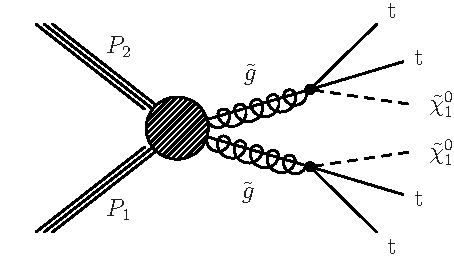
\includegraphics[width=0.32\textwidth]{figs/theory/T1tttt.pdf} \\
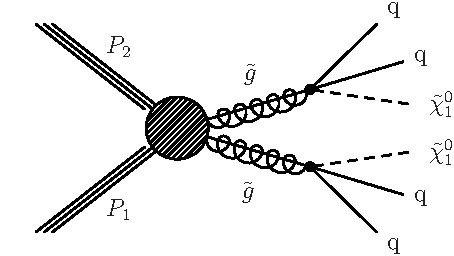
\includegraphics[width=0.32\textwidth]{figs/theory/T1qqqq.pdf} \\
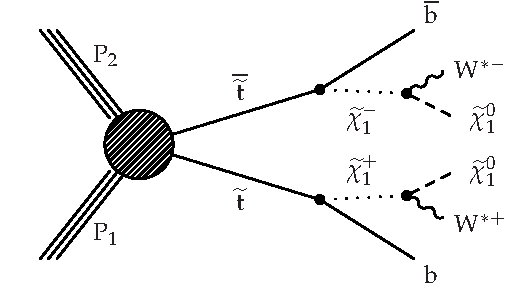
\includegraphics[width=0.32\textwidth]{figs/theory/T2bw.pdf}
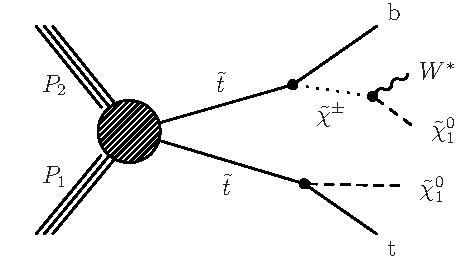
\includegraphics[width=0.32\textwidth]{figs/theory/T2tb.pdf}
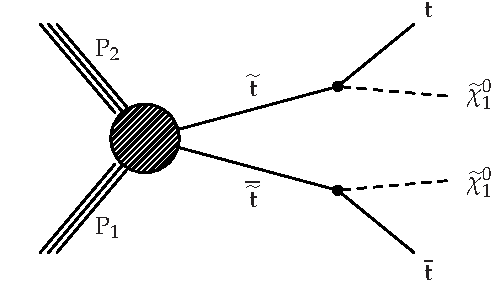
\includegraphics[width=0.32\textwidth]{figs/theory/T2tt.pdf}
\caption{Diagrams displaying the event topologies of gluino (upper 7
  diagrams) and top-squark (lower 3 diagrams) pair production
  considered in this thesis.\label{fig:SMSDiagrams}}
\end{figure*}

In addition, several simplified models are considered for
the production of top-squark pairs, in which each top squark decays to
one of the following final state:
 \begin{itemize}
\item a bottom quark and the NLSP;
\item a top quark and the LSP.
\end{itemize}

The corresponding Feynman diagrams are shown in
Fig.~\ref{fig:SMSDiagrams}.

\subsection{Technical Implentation in \PYTHIA}
To simplify the treatment of the sparticle decays in \PYTHIA v6.4.26, we directly implement three-body decays of
the form $\chipm_1 \to \chiz_1 f f^{\prime}$, with branching ratios
as shown in Table~\ref{tab:nlspbr}.
\begin{table}
\centering
\begin{tabular}{l|r}
decay mode & branching ratio \\\hline
$\chip_1 \to \chiz_1 u \bar d$ &  35.1\%\\
$\chip_1 \to \chiz_1 c \bar s$ &  35.1\%\\
$\chip_1 \to \chiz_1 e^+ \nu_e$ &  11.7\%\\
$\chip_1 \to \chiz_1 \mu^+ \nu_{\mu}$ &  11.7\%\\
$\chip_1 \to \chiz_1 \tau^+ \nu_{\tau}$ &  6.4\%
\end{tabular}
\caption{\label{tab:nlspbr}Table of branching ratios implemented in
  \PYTHIA v6.4.26 for the NLSP
  $\chipm_1$ in the simplified natural SUSY model considered in this chapter.}
\end{table}
\section{Kinematics of Supersymmetric Events}
\label{sec:kinematic}
The pair production of supersymmetric particles has a distinct
kinematic features.


The razor variables \MR and  \Rtwo are motivated by the generic process of the pair production of two
heavy particles (e.g., squarks or gluinos), each decaying to an
undetected particle (the stable, weakly interacting LSP $\chiz_1$)
plus visible particles. The LSP is assumed to escape without
detection, leading to an imbalance $\ptvecmiss$ in the momentum
perpendicular to the beam axis. Each event is treated as a dijet-like event
and the four-momenta of the two jets are used to compute \MR and $\MRT$, defined as
\begin{align}
 \label{eq:MRstar}
 \MR &\equiv
 \sqrt{
(\abs{\vec{p}^{j_{1}}}+\abs{\vec{p}^{j_{2}}})^2 -({p}^{j_1}_z+{p}^{j_2}_z)^2},\\
\MRT &\equiv \sqrt{ \frac{\ETm(\pt^{j_1}+\pt^{j_2}) -
\ptvecmiss \cdot
 (\ptvec^{\,j_1}+\ptvec^{\,j_2}) }{2}},
\end{align}
where $\vec{p}_{j_i}$, $\ptvec^{\,j_i}$, and
$p^{j_i}_z$ are the momentum of the $i$th jet, its
transverse component with respect to the beam axis, and its
longitudinal component, respectively, with $\ETm$ the magnitude of $\ptvecmiss$. While
$\MRT$ quantifies the transverse momentum imbalance,
$\MR$ estimates the mass scale of new-physics particle
production in the event. The razor dimensionless ratio is defined as
\begin{equation}
\R \equiv \frac{\MRT}{\MR}.
\end{equation}
\part{The LHC and CMS}
\label{part:lhccms}
\chapter{The Large Hadron Collider}
\label{ch:lhc}
The Large Hadron Collider (LHC) is a 27\unit{km} two-ring superconducting
proton accelerator and collider located at CERN, spanning the border between
France and Switzerland.  At design specifications, the LHC will collide
protons at a center-of-mass energy of 14\TeV and instantaneous
luminosity $10^{34} \unit{cm}^{-2} \unit{s}^{-1}$.
\begin{table*}
\centering
 \caption{Comparison between LHC design parameters and achieved
   parameters in 2012 and 2015.
 \label{tab:LHCparameters}}
\resizebox{\textwidth}{!}{
\begin{tabular}{|l|c|c|c|c|}
\hline 
Parameter & Unit & \textbf{Design} & \textbf{Achieved (2012)} & \textbf{Achieved (2015)} \\\hline
\multicolumn{5}{|c|}{\textbf{Beam Data}}\\\hline
Proton energy & [GeV] & 7000 & 4000 & 6500 \\\hline
Relativistic gamma factor $\gamma_r$ & & 7461 & 4263 & 6928 \\\hline
Number of particles per bunch $N_b$ & & $1.15\times10^{11}$ &
                                                        $1.6-1.7\times10^{11}$ & $1.15\times10^{11}$ \\\hline
Number of bunches $n_b$ & & 2808 & 1374 & 2244 \\\hline
Bunch spacing & [ns] & 25 & 50 & 25 \\\hline
%Longitudinal emittance ($4\sigma$) & [eV s] & 2.5 & & \\\hline
Transverse normalized emittance $\varepsilon_n$& [$\mu$m rad] & 3.75
                                   &2.5& $\geq2.7$\\\hline
Circulating beam current & [A] & 0.582 & 0.369&\\\hline
Stored energy per beam & [MJ] & 362 & 140 &\\\hline
\multicolumn{5}{|c|}{\textbf{Peak Luminosity Related Data}}\\\hline
$\beta^{\ast}$ at IP1 and IP5 & [m] &0.55 & 0.6 & 0.8 \\\hline
RMS bunch length $\sigma_z$& [cm] & 7.55 & $\geq 9$ &\\\hline
RMS beam size at IP1 and IP5 $\sigma^{\ast}$ & [$\mu$m] & 16.7 & 19 &\\\hline 
Half crossing angle at IP1 and IP5 $\theta_c/2$& [$\mu$rad] & $\pm142.5$ &
                                                               $\pm145.0$ & $\pm145.0$\\\hline
Geometric luminosity reduction factor $F$ & &0.836 & &\\\hline
Peak luminosity in IP1 and IP5 & [cm$^{-1}$s$^{-1}$] &
                                                       $1.0\times10^{34}$ & $7.7\times10^{33}$ & $5.2\times10^{33}$ \\\hline
Max. mean number of events per bunch crossing& & 19 & 40 & 17 \\\hline
\end{tabular}
}
\end{table*}

The LHC is the pinnacle of the accelerator
complex at CERN, pictured in Fig.~\ref{fig:LHCComplex}.  To accelerate
protons to a beam energy of 6.5\TeV in the LHC, a chain of smaller
accelerators are needed. Starting from bottle of hydrogen gas,
electrons are stripped from the hydrogen atoms by an electric field
and the resulting protons enter the Linac 2, which accelerates the
protons to 50\MeV. Subsequently, the Proton Synchrotron Booster (PSB), Proton Synchrotron (PS), and the
Super Proton Synchrotron (SPS) accelerate the protons to 1.4\GeV, 25\GeV, and 450\GeV, respectively, before they are finally injected
into the two LHC rings as counter-rotating beams.

\begin{figure}\centering
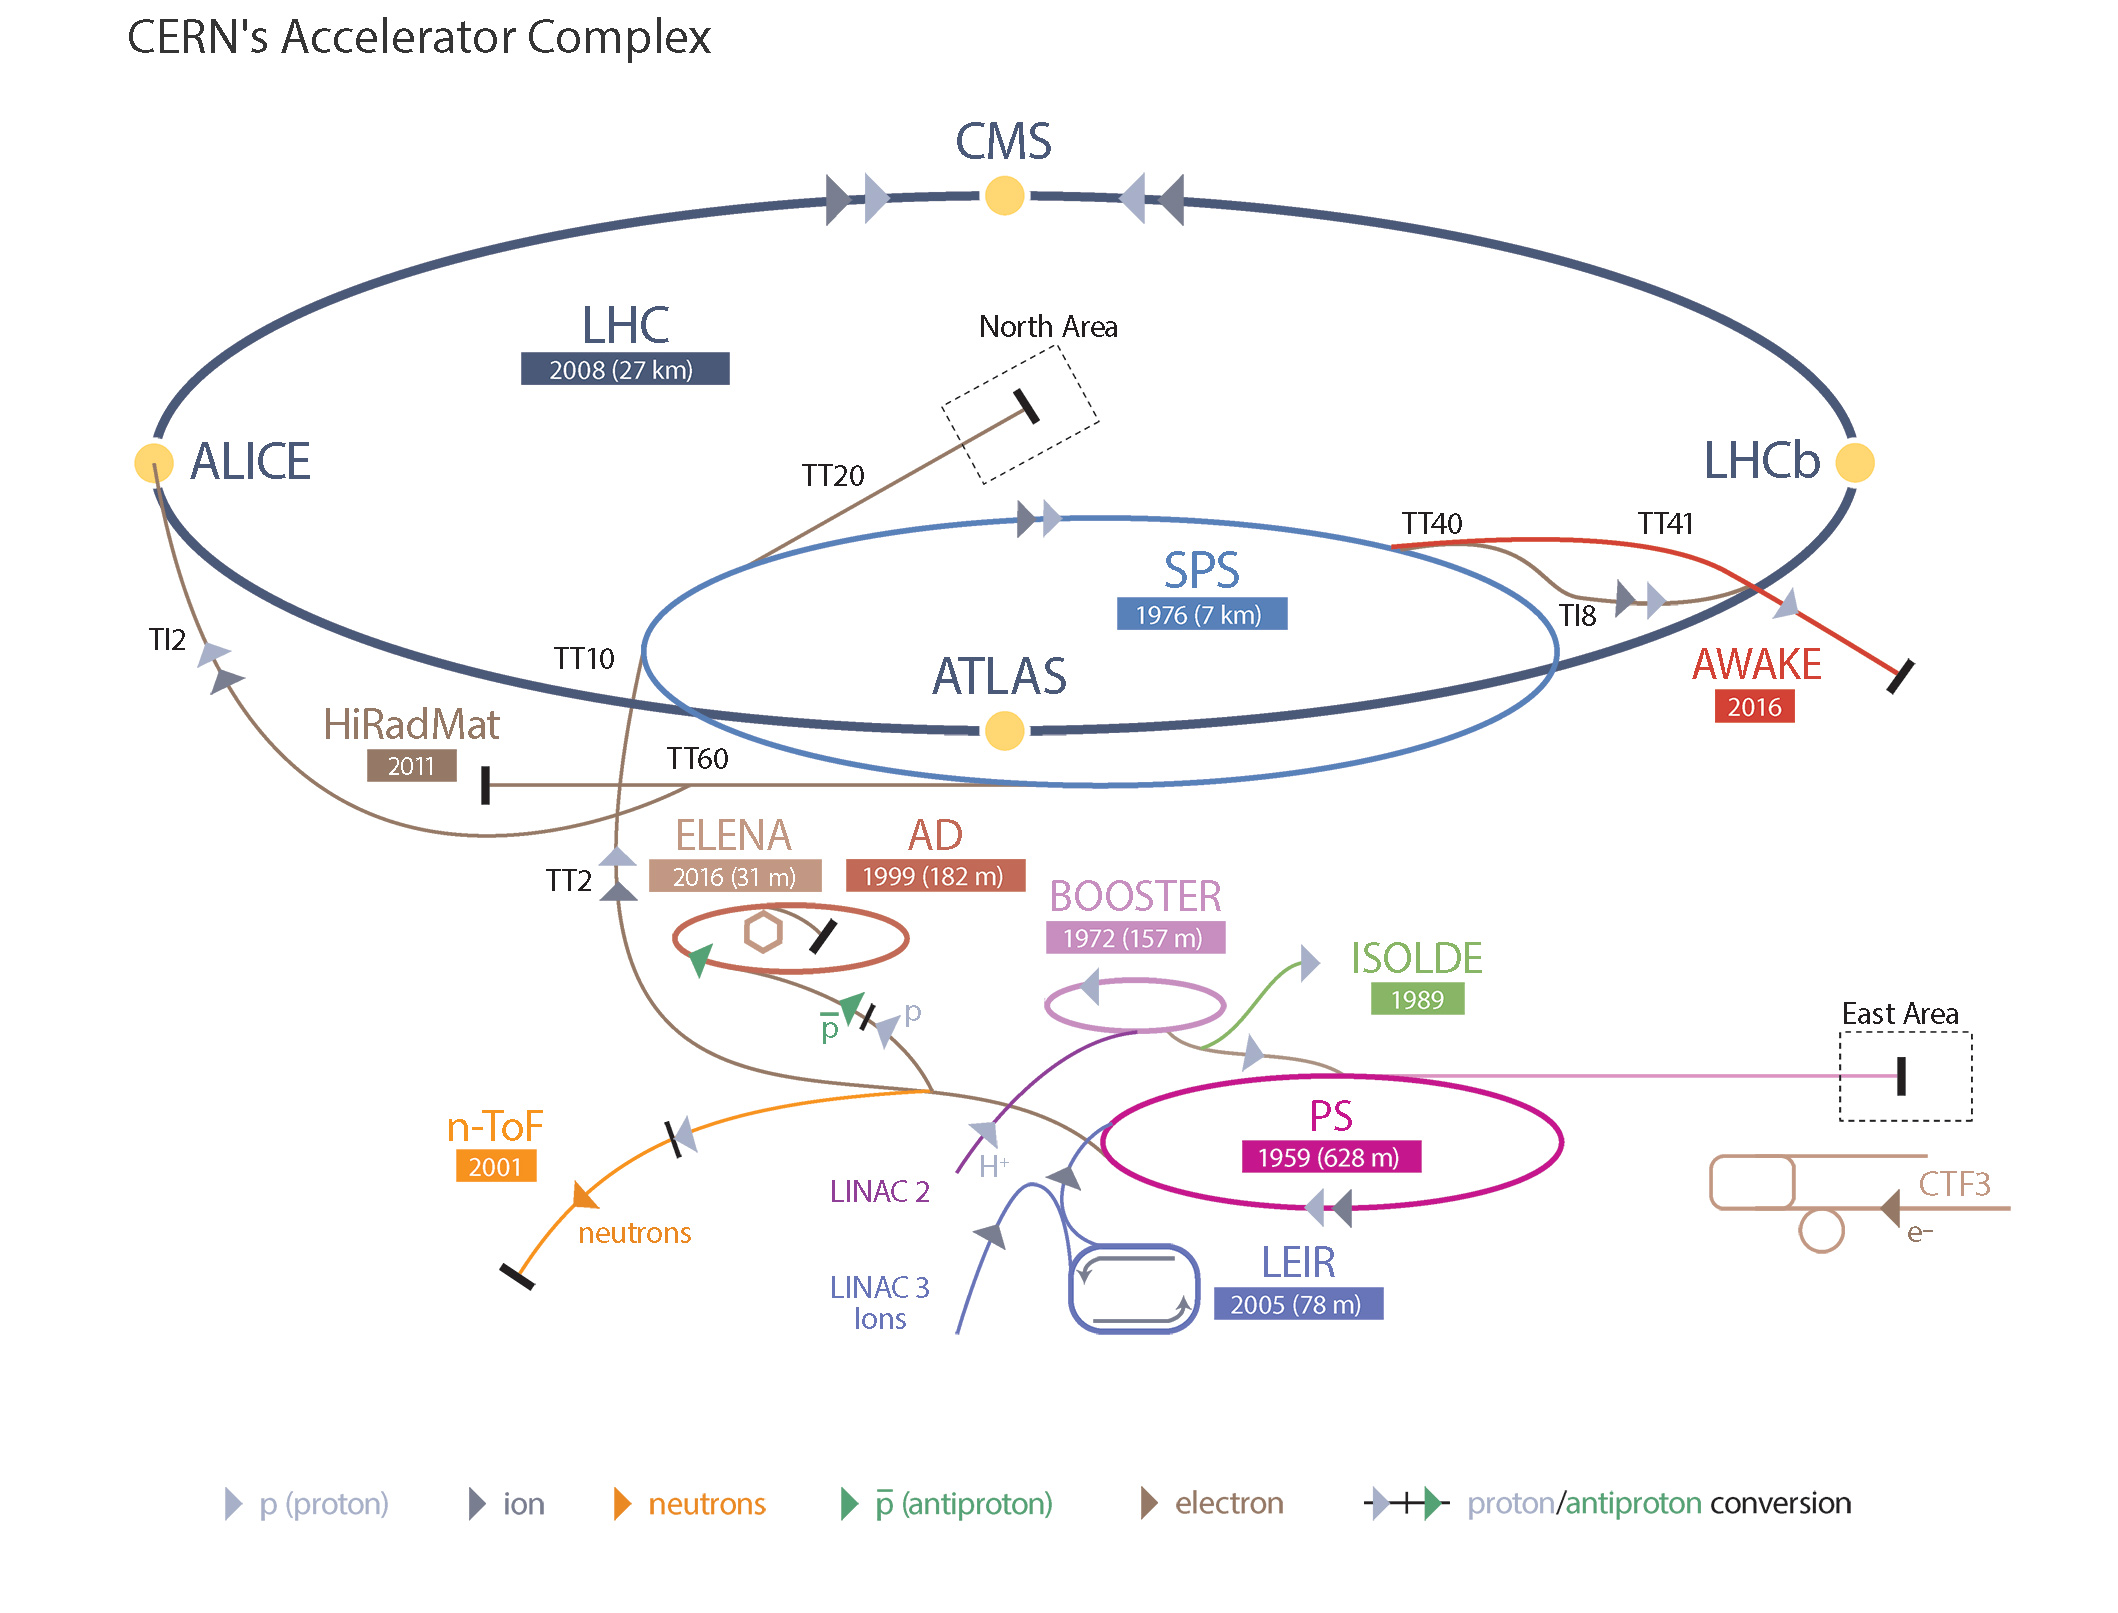
\includegraphics[width=.9\textwidth]{figs/cms/LHC_default.jpg}
\caption{CERN's accelerator complex.\label{fig:LHCComplex}}
\end{figure}

One of the main features influencing the design of the LHC is the re-use of the
existing 26.7\unit{km} tunnel from the Large Electron Positron collider (LEP), which is
comprised of eight crossing points (or arcs) and eight straight sections for
RF cavities. The tunnel in the arc sections has an internal diameter of 3.7\unit{m}. Due to the limited available space, two completely separate
proton rings with separate magnet systems would be extremely difficult to install, which makes the twin-bore magnet design proposed by John
Blewett in 1971~\cite{Blewett:1068131} ideal due to its
``two-in-one'' use of the limited space. A cross-section of the main superconducting
dipole magnet is shown in \ref{fig:LHCDipole}.

\begin{figure}\centering
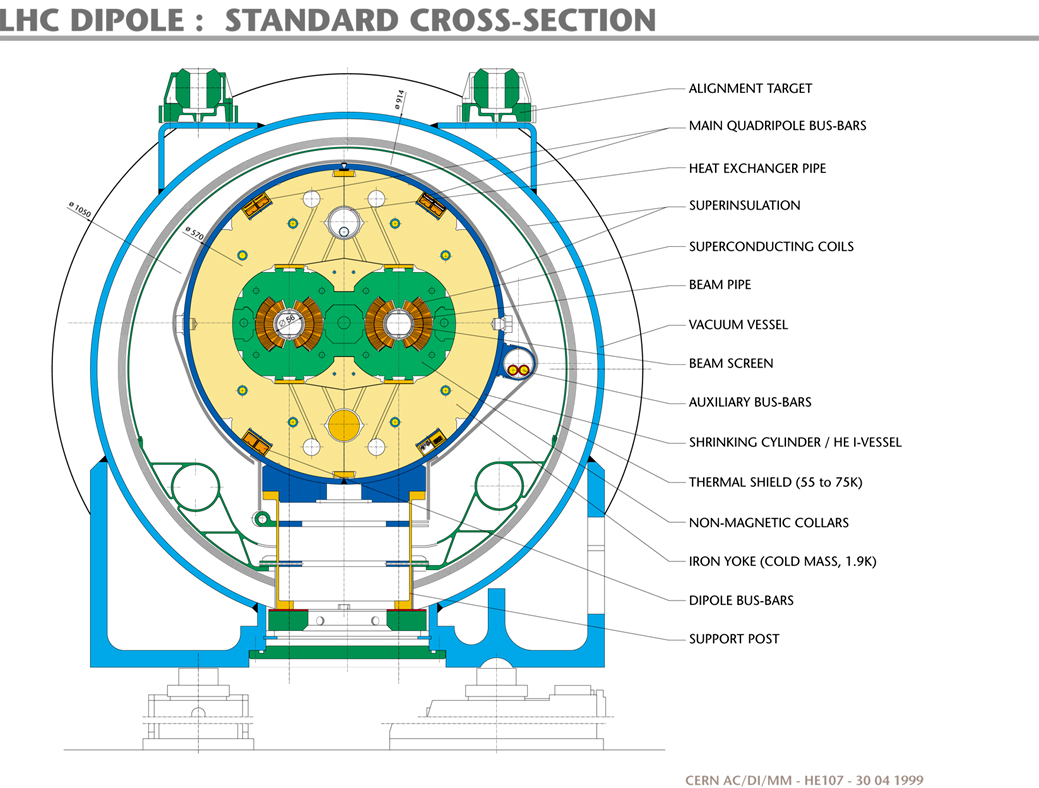
\includegraphics[width=.9\textwidth,clip=true,viewport=0 20 680 550]{figs/cms/lhc-pho-1999-172.jpg}
\caption{Cross-section of the LHC dipole magnet.\label{fig:LHCDipole}}
\end{figure}

The observed number of events $N_{\mathrm{exp}}$ is the product of the cross
section of interest $\sigma_{\mathrm{exp}}$ and the time integral of
the instantaneous luminosity,
\begin{equation}
N_{\mathrm{exp}}  =\sigma_{\mathrm{exp}}\int \mathscr{L}(t)dt ~.
\end{equation}
The instantaneous luminosity depends on the beam parameters and
can be written for a Gaussian beam distribution as~\cite{LHCMachine}:
\begin{equation}
\mathscr{L} =
\frac{N_b^2n_bf_{\mathrm{rev}}\gamma_r}{4\pi\varepsilon_n\beta^{\ast}}F~,
\label{eqn:instlumi}
\end{equation}
where $N_b$ is the number of particles per bunch, $n_b$ the number
of bunches per beam, $f_{\mathrm{rev}}$ the revolution frequency,
$\gamma_r$ the relativistic gamma factor, $\varepsilon_n$ the
normalized transverse beam emittance, $\beta^{\ast}$ the beta function
at the collision point, and $F$ the geometric luminosity reduction
factor due to the crossing angle at the interaction point (IP):
\begin{equation}
F=\left(1+\left(\frac{\theta_c\sigma_z}{2\sigma^{\ast}}\right)^2\right)^{-1/2}~,
\label{eqn:F}
\end{equation}
where $\theta_c$ is the full crossing angle, $\sigma_z$ is the RMS
bunch length, and $\sigma^{\ast}$ is the RMS bunch size.

The integrated luminosity of proton-proton collisions delivered by the
LHC to the CMS experiment versus time from $2010$ through $2016$ is
shown in Fig.~\ref{fig:IntLumi20102016}. The LHC also delivers lead-proton and
lead-lead collisions for one month each year to the experiments.

\begin{figure}\centering
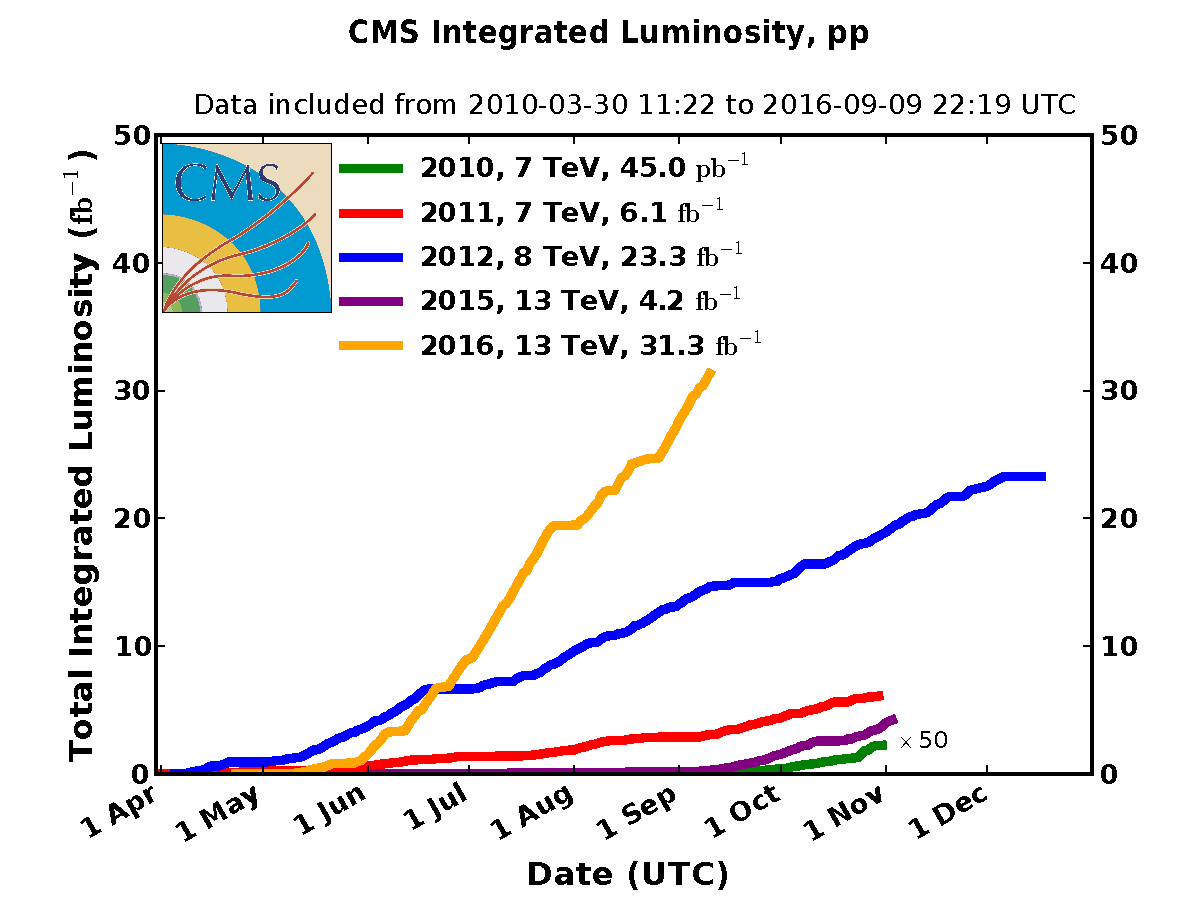
\includegraphics[width=.9\textwidth]{figs/cms/int_lumi_cumulative_pp_2.pdf}
\caption{Cumulative luminosity versus day delivered to CMS during
  stable beams for $\Pp\Pp$  collisions. This is shown for 2010 (green), 2011
  (red), 2012 (blue), 2015 (purple) and 2016 (orange)
  data-taking.\label{fig:IntLumi20102016}}
\end{figure}


\chapter{The CMS Experiment}
\label{ch:cms}
The Compact Muon Solenoid (CMS) detector is a multi-purpose detector
conceived to study proton-proton, proton-lead, and lead-lead collisions produced
by the Large Hadron Collider (LHC) at CERN~\cite{Adolphi:2008zzk}.

The ultimate goals of the LHC physics programme are to elucidate the nature of
electroweak symmetry breaking and search for evidence of new symmetries, new
forces, or new constituents of matter that could pave the way toward a
unified theory beyond the standard model. There are several detector
and readout requirements for CMS to meet these goals:
\begin{itemize}
\item Good muon identification and momentum resolution over a wide
  range of momenta, good dimuon mass resolution ($\approx 1\%$ at 100
  \GeV), and the ability to unambiguously determine the charge of muons
  with $p<1 \TeV$. See Sec.~\ref{sec:muon};
\item Good charged particle momentum resolution and reconstruction
efficiency in the inner tracker. Efficient triggering and offline
identification of $\Pgt$ leptons and \PQb-jets, requiring pixel
detectors close to the interaction region. See Sec.~\ref{sec:tracker};
\item Good electromagnetic energy resolution, good diphoton and
  dielecron mass resolution ($\approx 1\%$ at 100 \GeV), wide
  geometric coverage, $\pi^0$ rejection, and efficient photon and
  lepton isolation at high luminosities. See Sec.~\ref{sec:ecal};
\item Good missing-transverse-energy and dijet-mass resolution,
  requiring hadron calorimeters with hermetic geometric coverage and
  fine lateral segmentation. See Sec.~\ref{sec:hcal};
\item Fast online event selection process (\emph{trigger}) to reduce the rate from $10^9$ inelastic collision
  events per second to $\lesssim1000$ events per second for storage
  and subsequent analysis. See Sec.~\ref{sec:trigger};
\item Infrastructure for the alignment and calibration of the detector. See Sec.~\ref{sec:alca}.
\end{itemize}

The design of CMS, pictured in Fig.~\ref{fig:CMSperspective} and detailed
in the following sections, meets these requirements. Each detector subsystem is
integral to the performance of CMS as a whole and is specialized to a
particular class of particles, as seen in Fig.~\ref{fig:CMSslice}: the silicon
tracker measures the tracks of charged particles, the electromagnetic
calorimeter measures the energy of electrons and photons, the hadron calorimeter measures the
energy of charged and neutral hadrons, and the muon detectors
identify and measure the momentum of muons.

All of the subdetectors are built around the central feature of the
CMS detector, which is a superconducting solenoid providing a uniform axial
magnetic field of 3.8\unit{T}  over a magnetic length of 12.5 \unit{m}
and a free-bore radius of 3.15 \unit{m}. The large bending power ($11.4$ \unit{T}\unit{m}) of the
superconducting magnet permits a precise measurement of the momentum
of high-energy charged particles in silicon tracker. The return field is large enough to
saturate $1.5$ \unit{m} of iron, allowing four \emph{muon stations} to be
integrated and the bore of the magnet coil is large enough to accommodate the inner tracker
and the calorimetry inside, thereby minimizing the amount of material
in front of the calorimeters.

%The central feature of the CMS detector is a
%superconducting solenoid of 6\unit{m} internal diameter, providing a
%magnetic field of 3.8\unit{T}. Within the superconducting solenoid
%volume are a silicon pixel and a silicon strip tracker, a
%lead-tungstate crystal electromagnetic calorimeter, and a
%brass/scintillator hadron calorimeter, each composed of a barrel and
%two endcap sections. Muons are measured in gas-ionization detectors
%embedded in the magnet steel flux-return yoke outside the
%solenoid. Extensive forward calorimetry complements the coverage
%provided by the barrel and endcap detectors. Jets and leptons are
%reconstructed within the pseudorapidity region $\abs{\eta}<3$, covered by the
%electromagnetic and hadron calorimeters. Muons are reconstructed with
%$\abs{\eta}<2.4$. Events are selected by a two-level trigger system. The first level (L1) is based on a hardware
%filter, followed by a software-based high-level trigger (HLT). 

\begin{figure}\centering
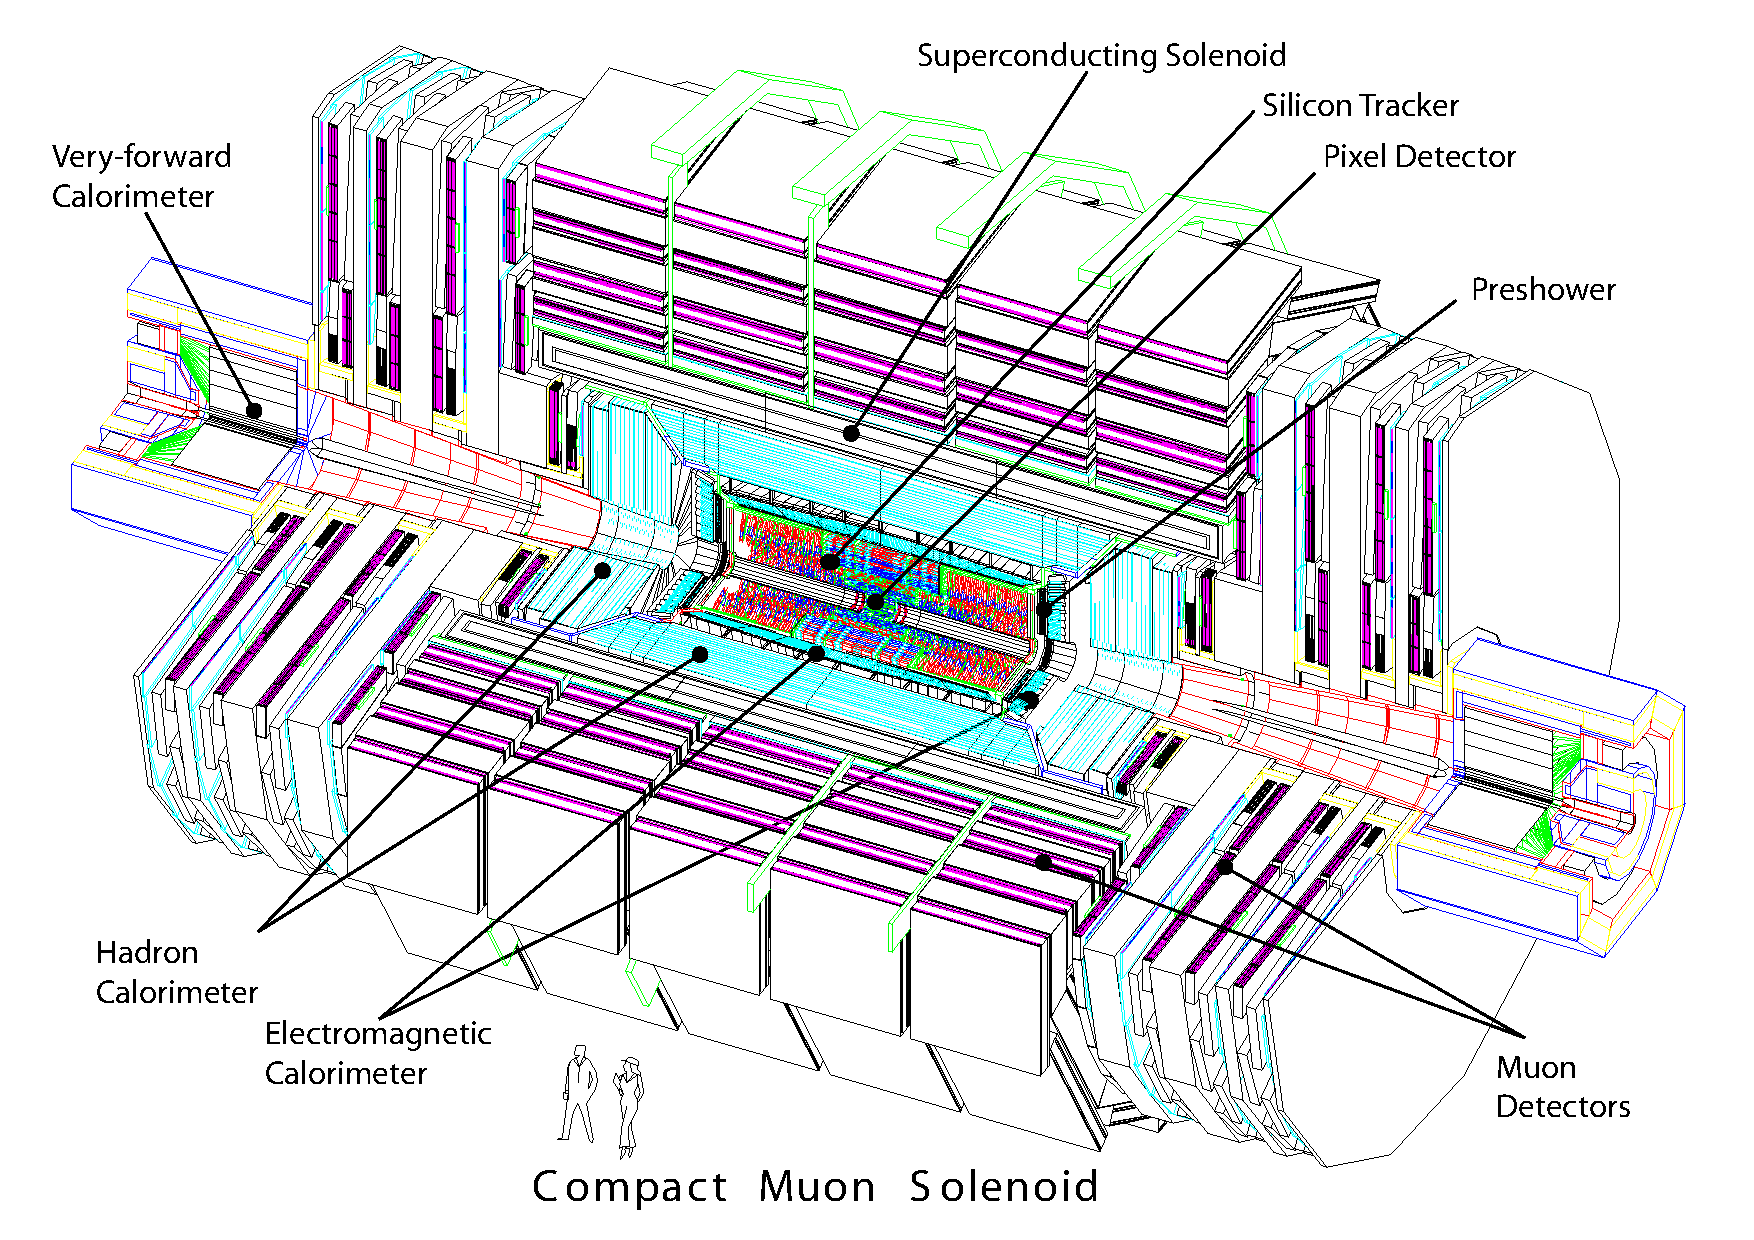
\includegraphics[width=.9\textwidth]{figs/cms/Figure_001-002.pdf}
\caption{Perspective view of the CMS detector.\label{fig:CMSperspective}}
\end{figure}

\begin{figure}\centering
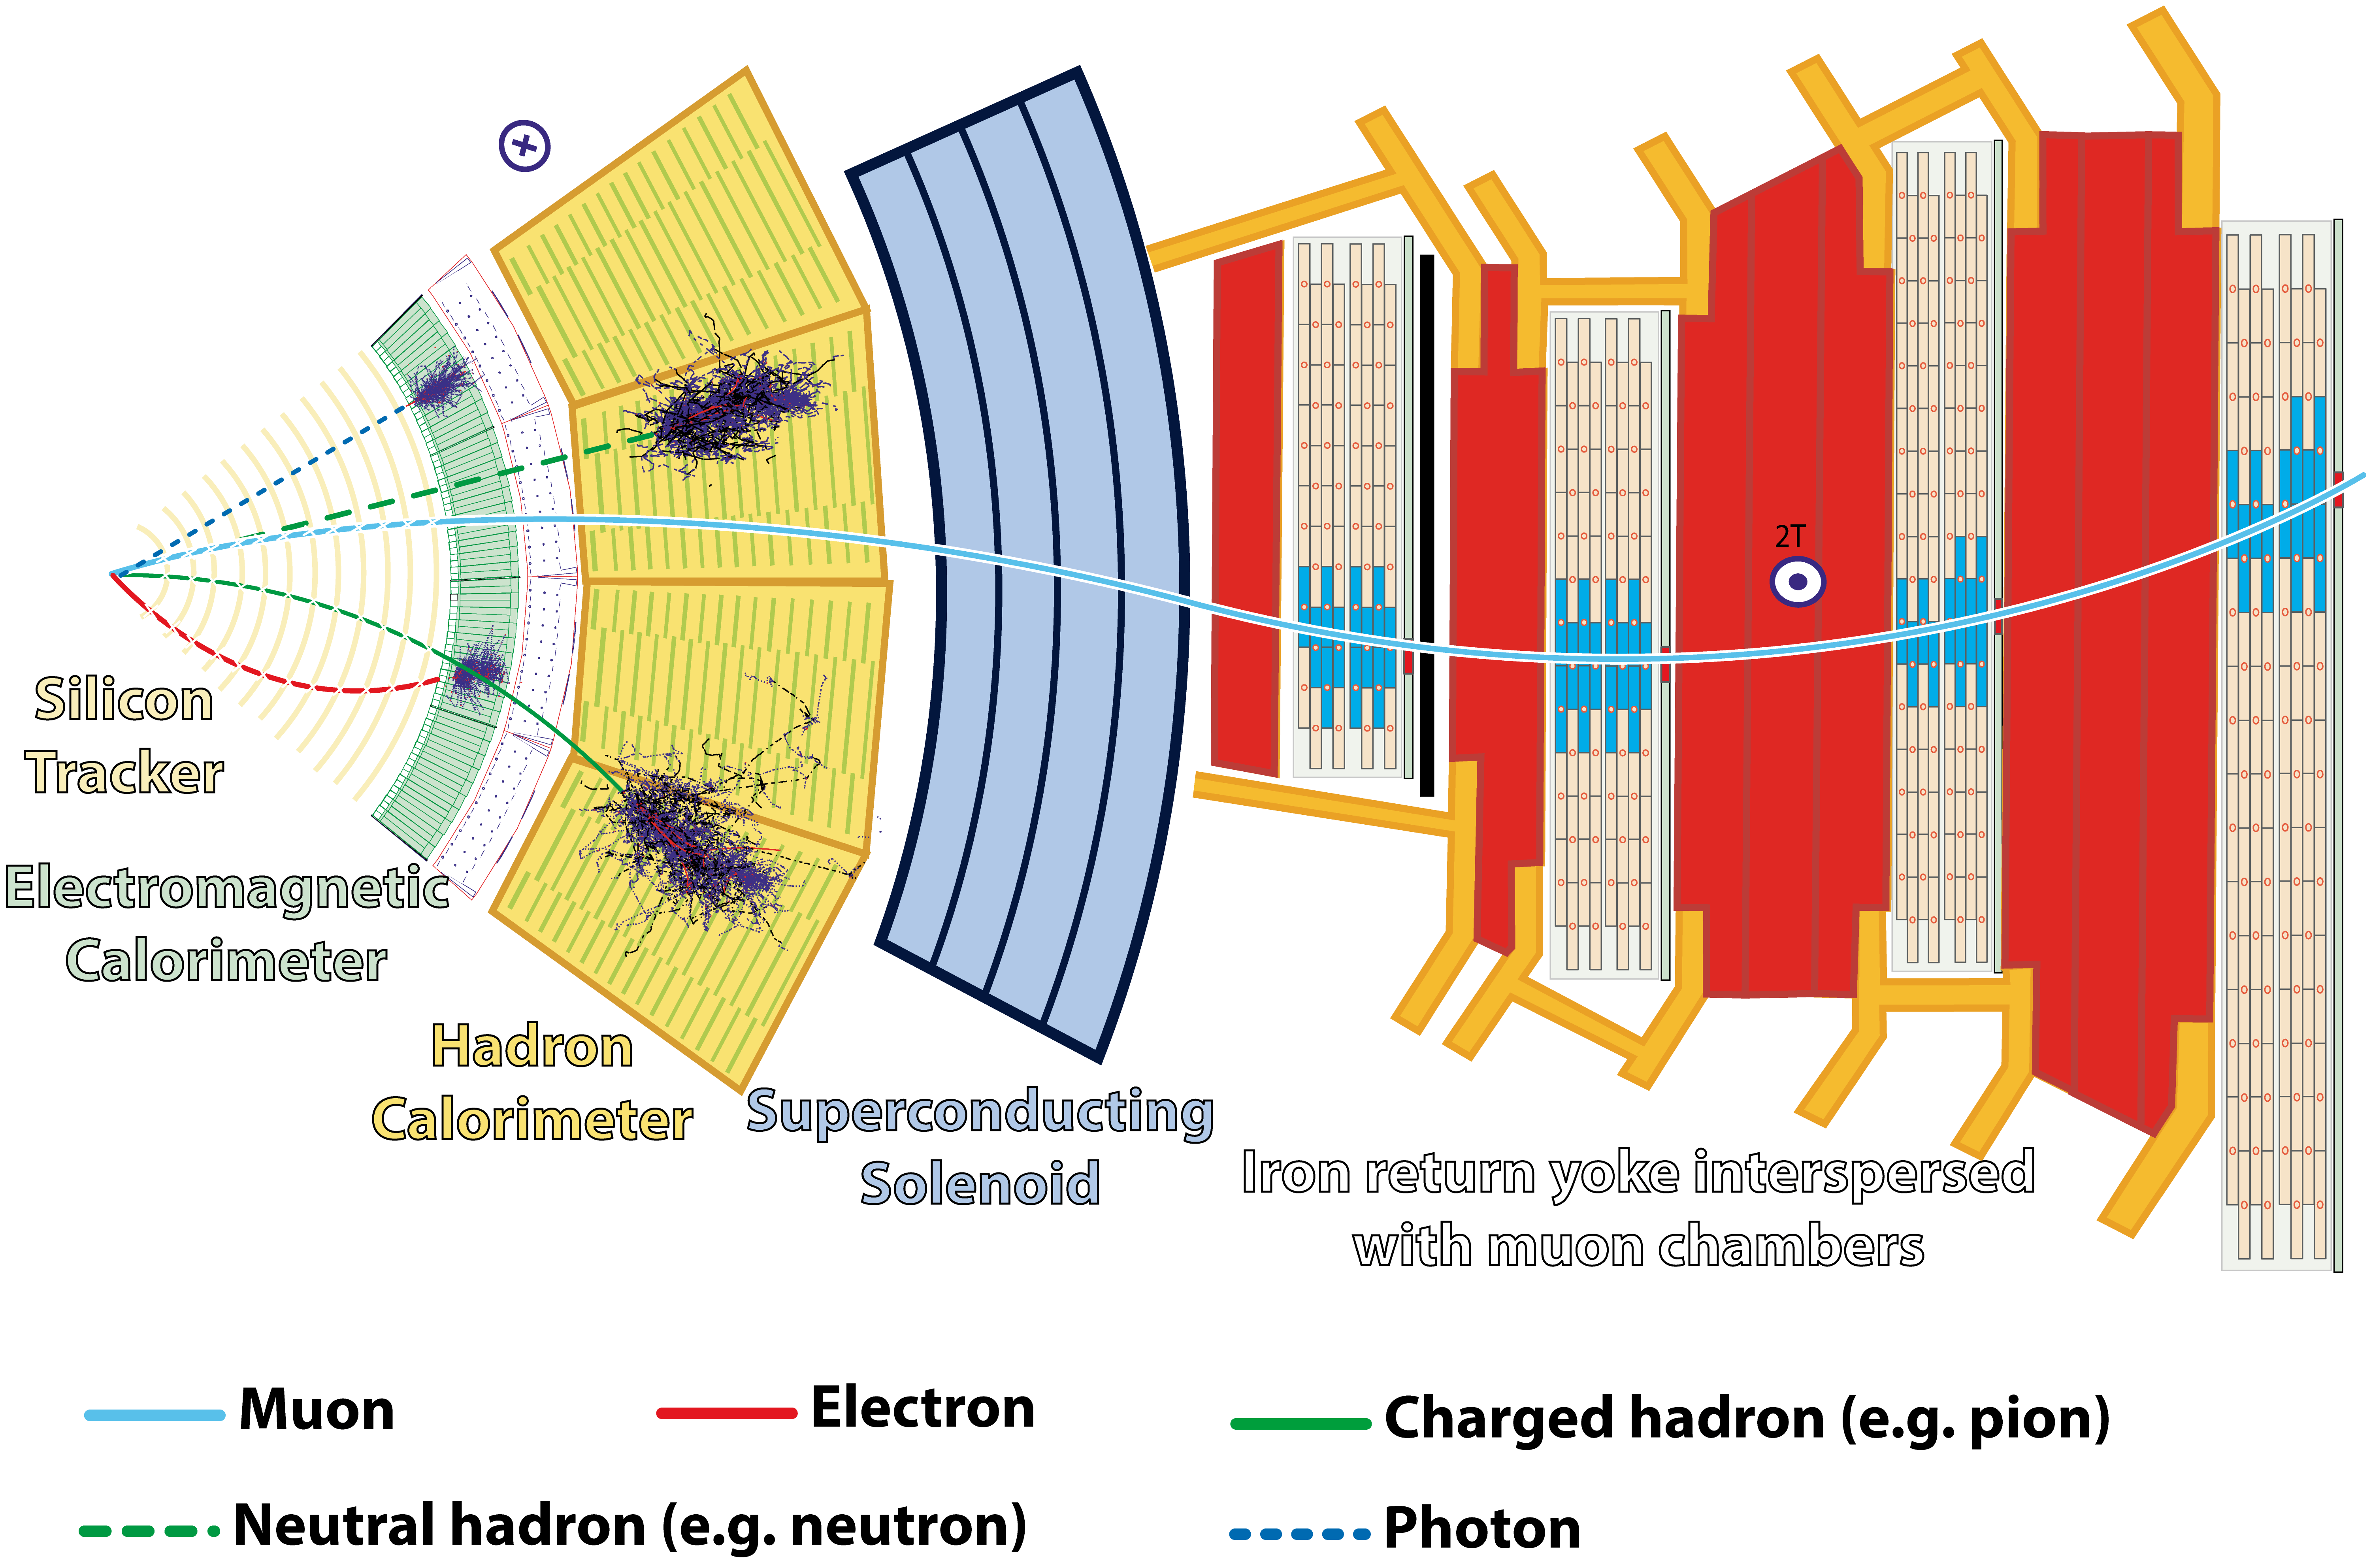
\includegraphics[width=.9\textwidth]{figs/cms/CMSslice_whiteBackground.png}
\caption{A slice of the CMS detector.\label{fig:CMSslice}}
\end{figure}


\section{Silicon Tracker}
\label{sec:tracker}
The first layer of the detector encountered by outgoing particles from the
collisions is the tracker, composed of a small silicon pixel
surrounded by a large silicon strip tracker~\cite{Chatrchyan:2014fea}. Both tracker subdetectors are
cylinder-shaped and occupy a total $5.8$ \unit{m} in length and $2.5$
\unit{m} in diameter. The pixel detector barrel (endcaps) comprises three (two) layers of pixel
detectors, providing three-dimensional position measurements of the
hits arising from the interaction of charged particles with its
sensors. The hit position resolution is approximately $10$ $\mu$m in
the transverse coordinate and $20–40$ $\mu$m in the longitudinal
coordinate, while the third coordinate is given by the sensor plane
position. In total, its $1440$ modules cover an area of about 1
m$^{2}$ and have $66$ million pixels.

%The pixel detector consists of cylindrical barrel layers at radii of 4.4, 7.3 and 10.2 cm, and two pairs of endcap disks at z = ±34.5 and ±46.5 cm. It provides three-dimensional (3-D) position measurements of the hits arising from the interaction of charged particles with its sensors.

Surrounding this is the silicon strip tracker. The silicon detector
barrel (endcaps) has ten (twelve) layers of micro-strip detectors. In
total, the with
$15,148$ silicon modules, which cover an active area of about $198$
m$^2$ and have $9.3$ million strips. 

%It is composed of four subsystems. The Tracker Inner Barrel (TIB) and Disks
%(TID) cover r < 55 cm and |z| < 118 cm, and are composed of four
%barrel layers, supplemented by three disks at each end. These provide
%position measurements in rφ with a resolution of approximately 13–38
%μm. The Tracker Outer Barrel (TOB) covers r > 55 cm and |z| < 118 cm
%and consists of six barrel layers providing position measurements in
%rφ with a resolution of approximately 18–47 μm. The Tracker EndCaps
%(TEC) cover the region 124 < |z| < 282 cm. Each TEC is composed of
%nine disks, each containing up to seven concentric rings of silicon
%strip modules, yielding a range of resolutions similar to that of the
%TOB.

The fine granularity of the two tracker subdetectors offers separation of closely-spaced particle
trajectories in energetic jets. Fig.~\ref{fig:tracker} shows a
schematic layout of the tracker in the $r-z$ plane and
the material budget of the CMS tracker, both in units of radiation
lengths and nuclear interaction lengths, as estimated from
simulation. Due to the tracker's material budget, a consistent fraction of
electrons and photon begin showering already in the tracker, which
implies the need for a global strategy to event reconstruction
(detailed in Sec.~\ref{sec:pf}).

%The simulation describes the tracker material budget with
%an accuracy better than 10\%, as was established by measuring the
%distribution of reconstructed nuclear interactions and photon
%conversions in the tracker.

\begin{figure}\centering
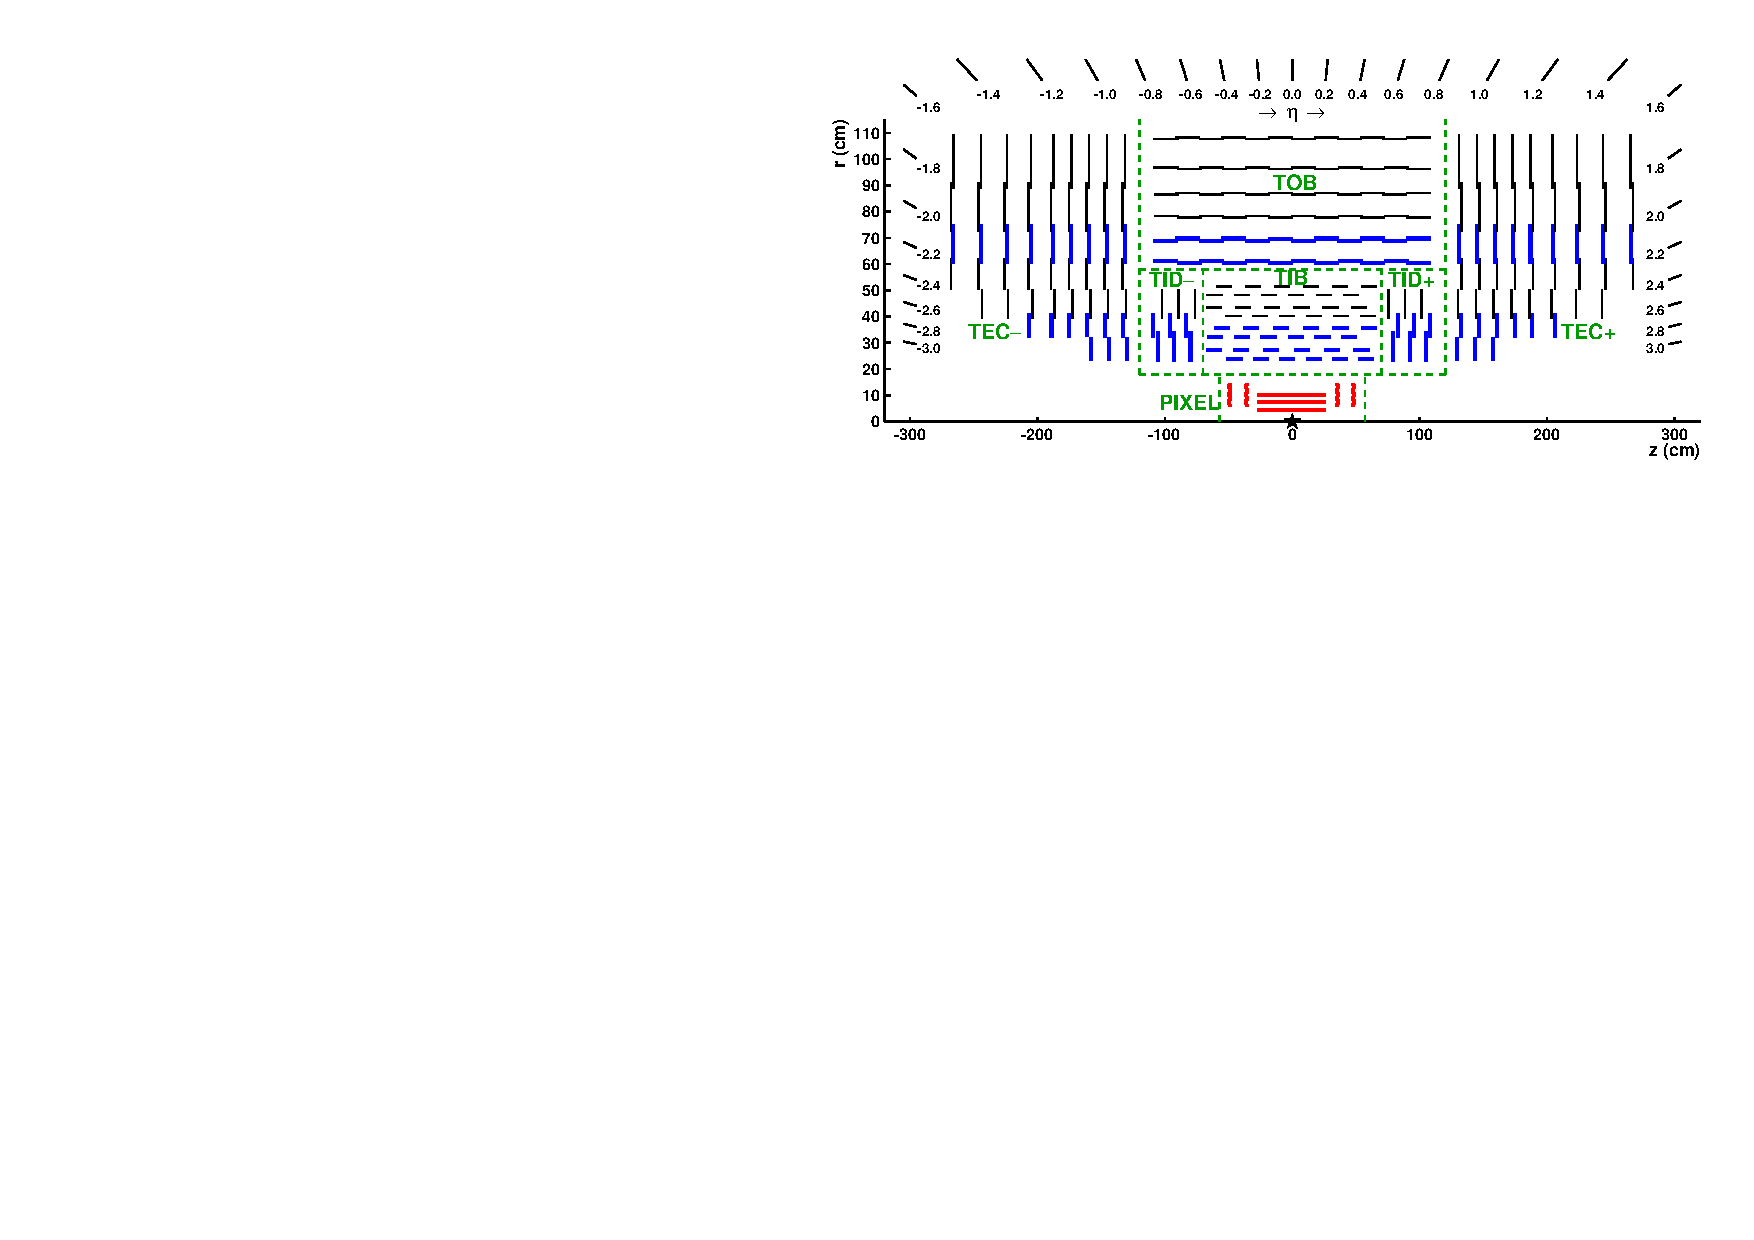
\includegraphics[width=.9\textwidth]{figs/cms/TrackerLayoutNew.pdf}\\
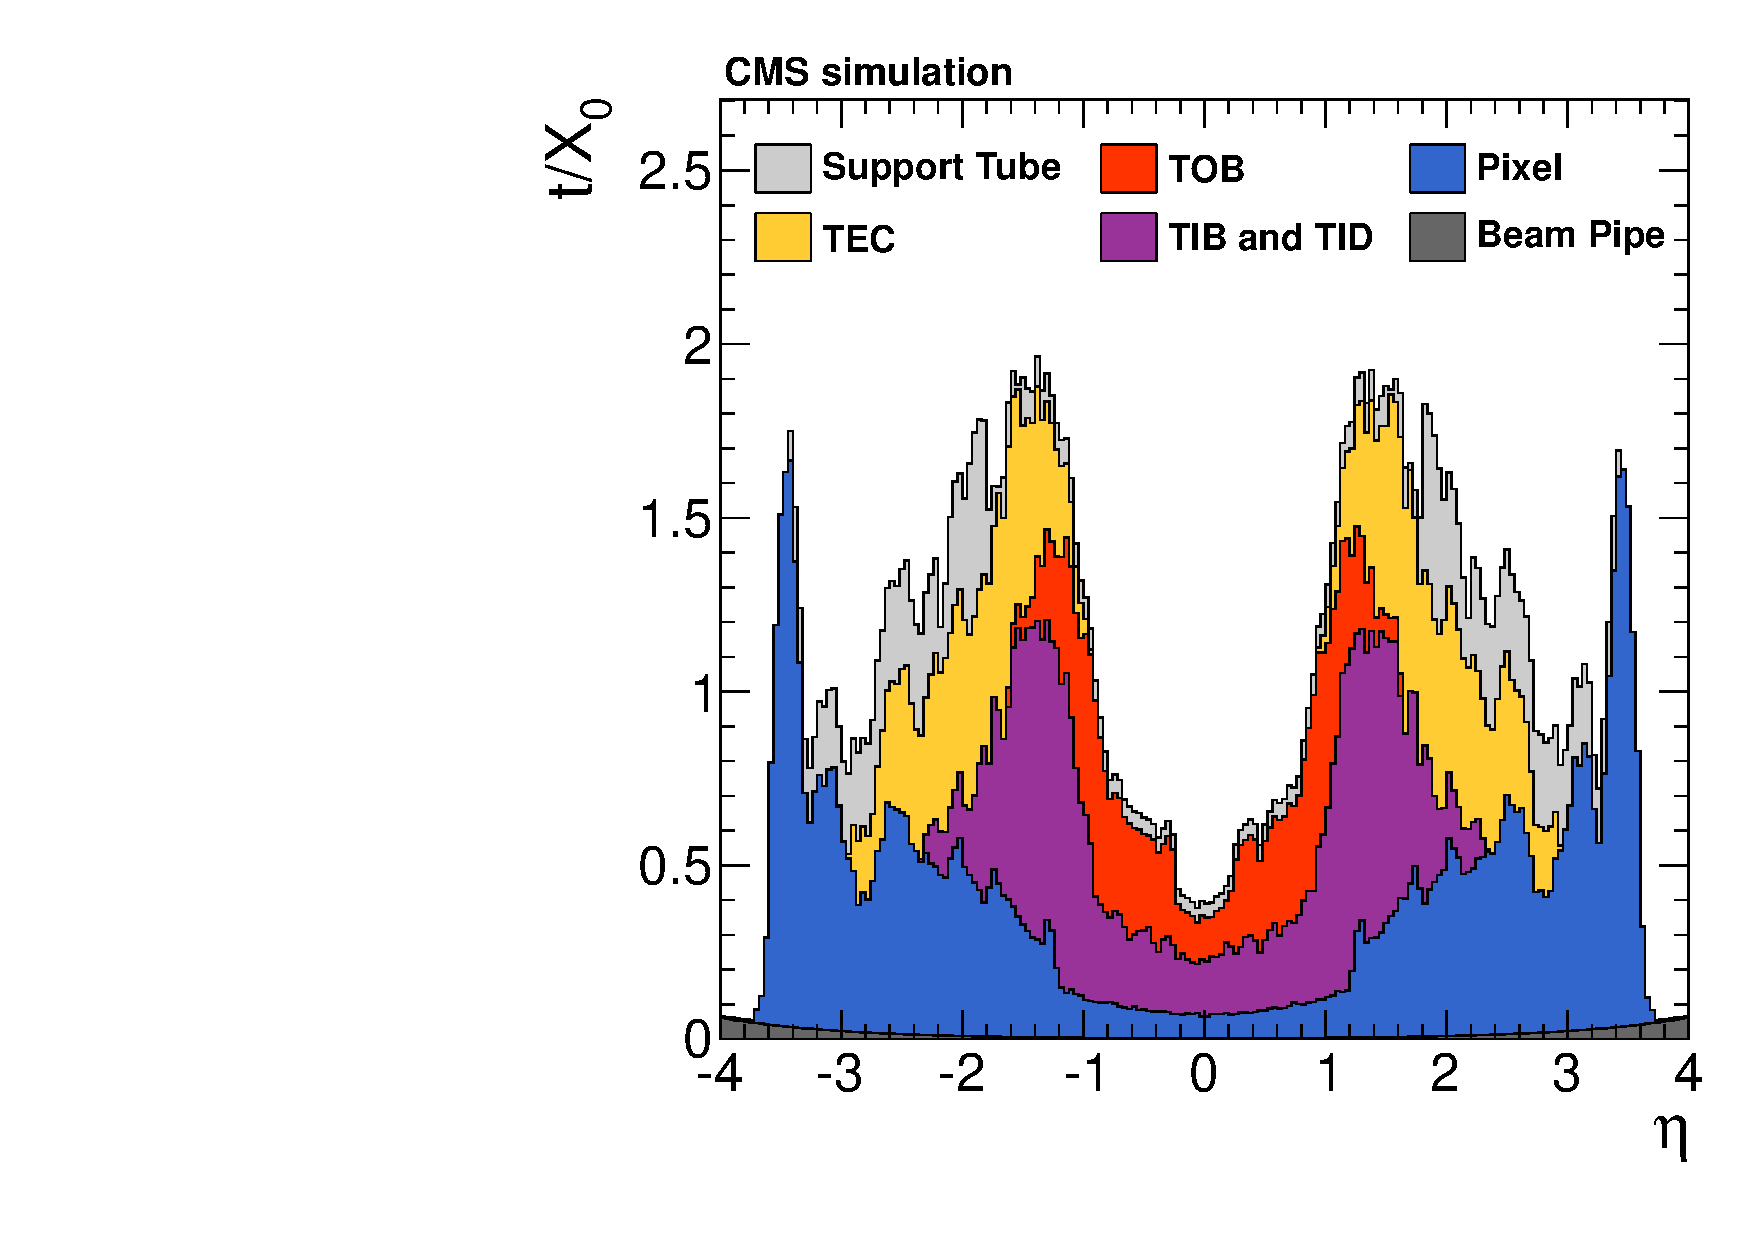
\includegraphics[width=.45\textwidth]{figs/cms/MaterialBudget_RadLengths.pdf}
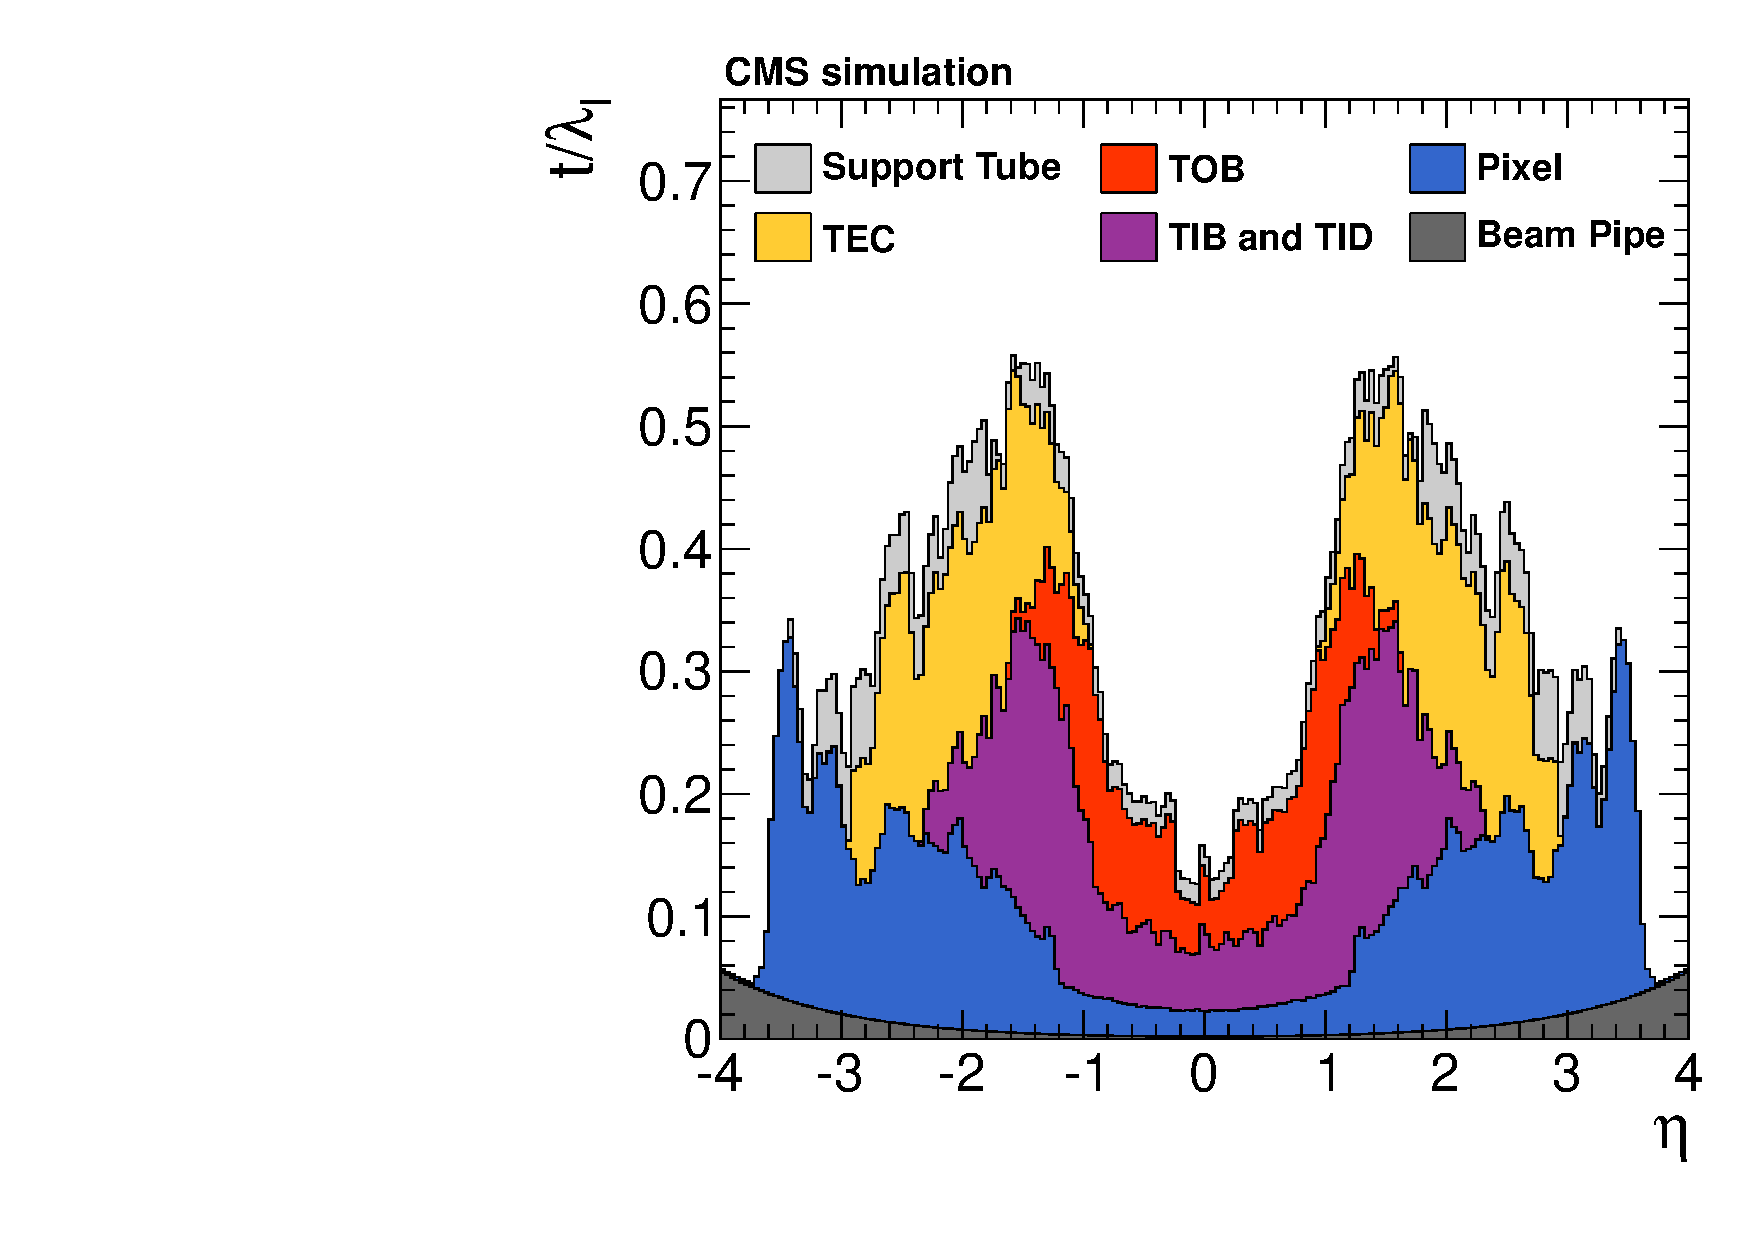
\includegraphics[width=.45\textwidth]{figs/cms/MaterialBudget_InteractionLengths.pdf}
\caption{(Top) Schematic cross section through the CMS tracker in the $r-z$
  plane. (Bottom) Total thickness $t$ of the tracker material
  traversed by a particle produced at the nominal interaction point,
  as a function of pseudorapidity $\eta$, expressed in units of radiation
  length $X_0$ (left) and nuclear interaction length $\lambda_I$
  (right). \label{fig:tracker}}
\end{figure}

%In this view, the tracker is symmetric about the horizontal
%  line $r = 0$, so only the top half is shown. The center of the
%  tracker, corresponding to the approximate position of the pp
%  collision point, is indicated by a star. Green dashed lines help the
%  reader understand which modules belong to each of the named tracker
%  subsystems. Strip tracker modules that provide 2D hits are shown by
%  thin, black lines, while those permitting the reconstruction of hit
%  positions in 3D are shown by thick, blue lines. The latter actually
%  each consist of two back-to-back strip modules, in which one module
%  is rotated through a `stereo' angle. The pixel modules, shown by the
%  red lines, also provide 3D hits. Within a given layer, each module
%  is shifted slightly in $r$ or $z$ with respect to its neighboring
%  modules, which allows them to overlap, thereby avoiding gaps in the
%  acceptance.


\section{Electromagnetic Calorimeter}
\label{sec:ecal}

Within the superconducting solenoid volume and just outside of the
tracker, lies the electromagnetic calorimeter (ECAL) schematically
pictured in Fig.~\ref{fig:ecal}. The ECAL is a hermetic homogenous
calorimeter composed of 61,200 lead-tungstate (PbWO$_{4}$) scintillating crystals mounted in
the barrel covering $\abs{\eta}<1.479$, and 7,324 crystals mounted in the two endcap disks
covering $1.479<\abs{\eta}<3.0$. The crystals in the barrel are arranged in a
quasi-projective geometry, meaning that they point back to the center of the detector.
The high-density ($8.28$ g/cm$^{3}$),
short radiation length ($X_0 = 0.89$ cm), and small Moli\'{e}re radius
($R_M$ = 2.2 cm) of PbWO$_{4}$ allow the construction of a compact
calorimeter with fine granularity.

\begin{figure}
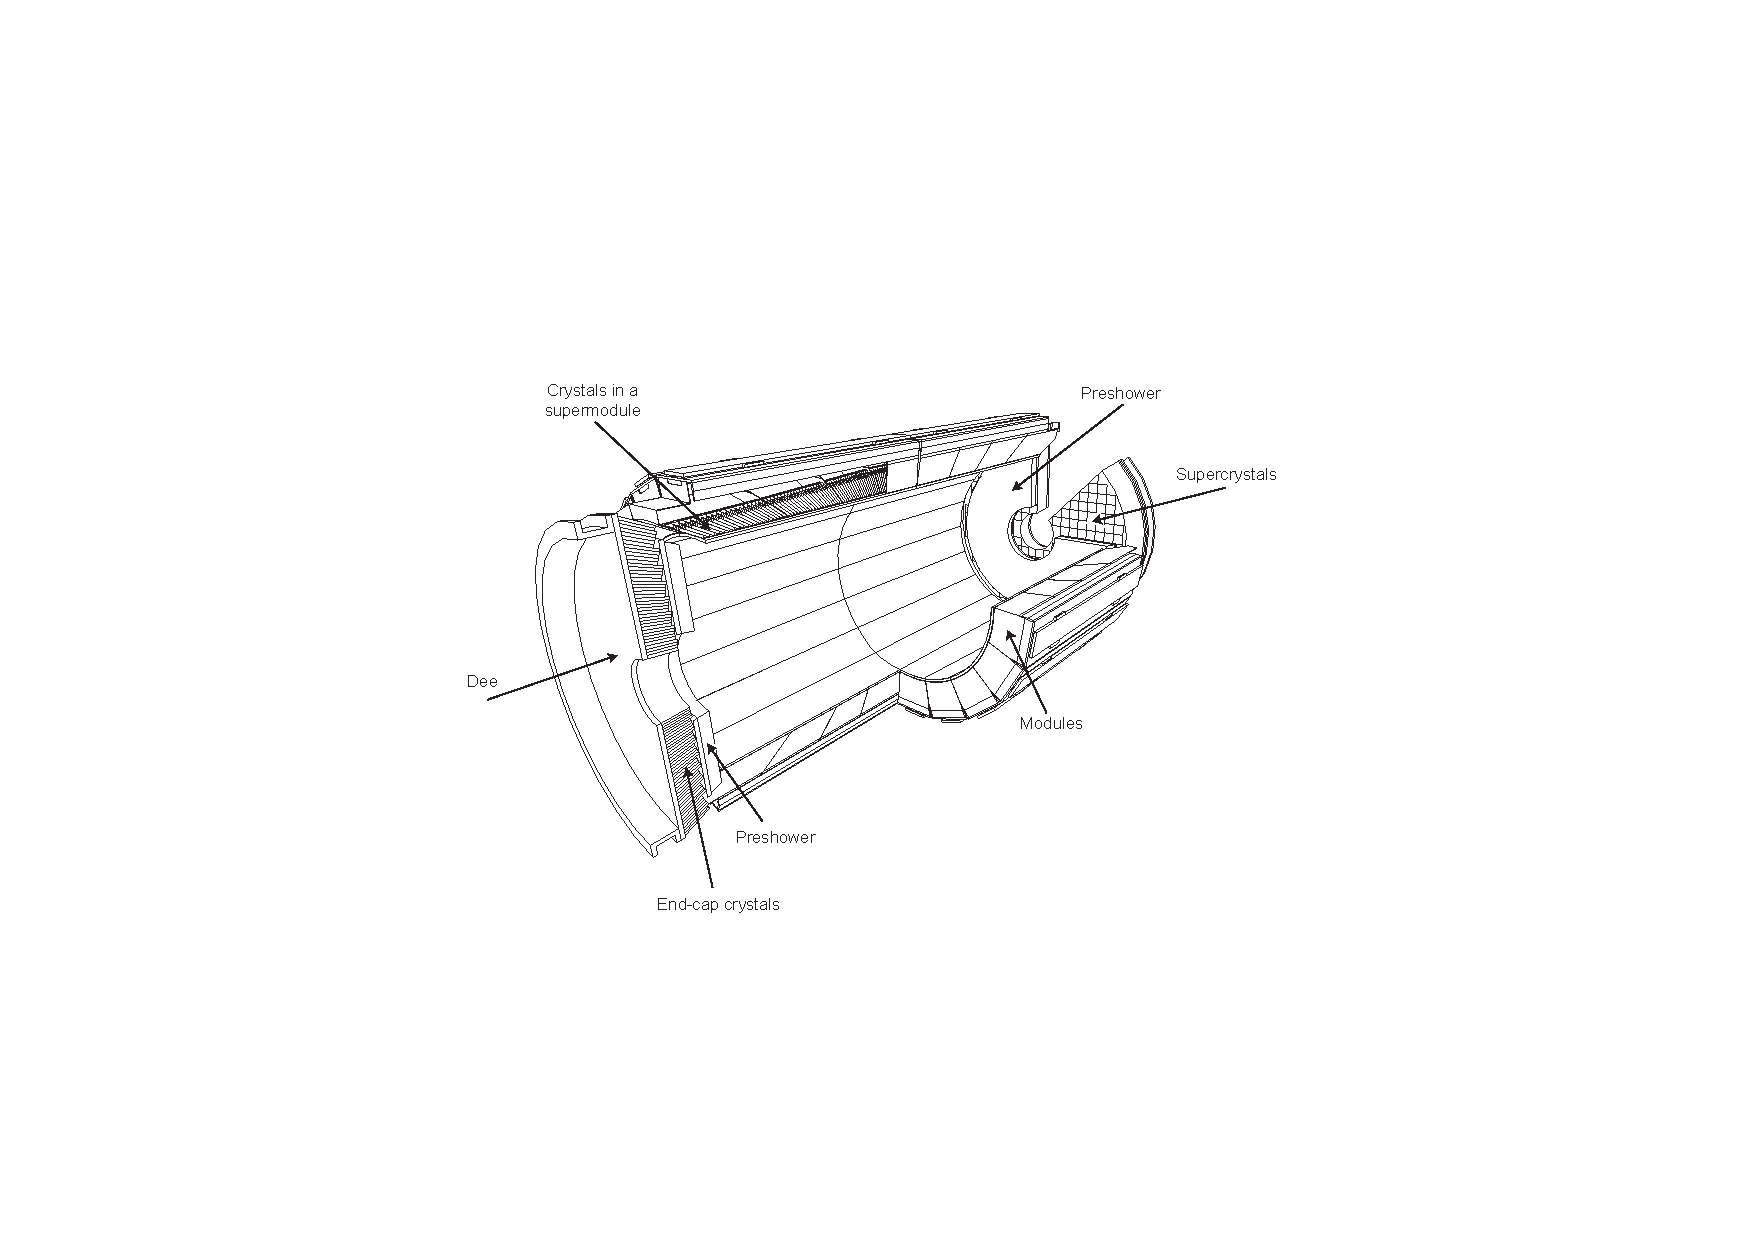
\includegraphics[width=.9\textwidth]{figs/cms/calorimeter.pdf}\centering
\caption{Layout of the CMS ECAL, showing the barrel supermodules, the
  two endcaps and the preshower detectors. The ECAL barrel coverage is
  up to $\abs{\eta} = 1.48$; the endcaps extend the coverage to $\abs{\eta} = 3.0$; the
  preshower detector fiducial area is approximately $1.65 < \abs{\eta}
  < 2.6$.\label{fig:ecal}}
\end{figure}

The crystal length of $23$ ($22$) \unit{cm}, corresponding to $25.8$
($24.7$) radiation lengths in the barrel (endcaps), is sufficient to
contain more than 98\% of the energy of electrons and photons up to
$1$ \TeV. The crystal material also amounts to about one nuclear interaction
length, causing about two thirds of the hadrons to start showering in
the ECAL.

The barrel crystal front face has an area of  $2.2 \times 2.2$ cm$^2$, equivalent to $0.0174 \times 0.0174$ in the ($\eta,\phi$)
plane, while in the endcaps, the crystals are arranged instead in a
rectangular ($x, y$) grid, with a front-face area of $2.9 \times 2.9$
cm$^{2}$. The crystal transverse size in the barrel matches the small Moli\`{e}re radius of
PbWO$_4$ ($2.2$ cm). This fine transverse granularity makes it possible to fully resolve hadron and photon
energy deposits as close as $5$ \unit{cm}. 
% for the benefit of exclusive particle identification in jets up to
% very large transverse momentum. 

The PbWO$_4$ crystals emit blue-green scintillation light with a broad
maximum at wavelengths $420–430$ \unit{nm}. The quantum efficiency and surface
coverage of the photodetectors are such that a particle depositing $1$
\unit{MeV} of energy in a crystal produces an average signal of about
$4.5$ photoelectrons.
% The stability of the temperature
%and of the photodetector gain are critical for an accurate
%determination of the energy deposited in the crystals.

The ECAL barrel energy resolution for electrons is measured in
an electron test beam to be~\cite{Adzic:2007mi,Chatrchyan:2013dga},
\begin{align}
\frac{\sigma_E}{E} &= \frac{S}{\sqrt E (\GeV)} \oplus \frac{N}{E (\GeV)} \oplus C \\
&= \frac{2.8\%}{\sqrt E (\GeV)} \oplus \frac{12\%}{E (\GeV)} \oplus 0.3\%
\end{align}
%\\&= \frac{7\%}{\sqrt E (\GeV)} \oplus \frac{35\%}{E (\GeV)} \oplus 0.7\%
where the three contributions are the stochastic, noise, and constant
terms.

A finer-grained detector, known as the preshower, is installed in
front of each endcap disks. It consists of two layers, each comprising
a lead radiator followed by a plane of silicon strip sensors, with a
pitch of $1.9$ \unit{mm}. The goal of the preshower is to enhance photon
identification capabilities.

Since ECAL crystals are approximately one Moli\'ere radius in lateral
dimension, high energy electromagnetic showers spread laterally over
several crystals. 
%Furthermore, in CMS, the presence of material in
%front of the electromagnetic calorimeter (corresponding to 1--2$\,X_0$
%depending on the $\eta$ region) causes conversion of photons and
%bremsstrahlung from electrons. The strong magnetic field of the
%experiment tends to spread this radiated energy along $\phi$.
Clustering algorithms are used to sum together energy
deposits in adjacent crystals belonging to the same electromagnetic
shower. The clustering algorithm proceeds first with the formation of ``basic clusters'', corresponding
to local maxima of energy deposits. The basic clusters are then merged
together to form a ``supercluster,'' which is extended in
$\phi$ (because charged particle tracks bend in $\phi$, but not in
$\eta$), to recover the radiated energy. Because of the differences
between the geometric arrangement of the crystals in the barrel and
endcap regions, a different clustering algorithm is used in each
region. The clustering algorithm used in the barrel, called the ``hybrid''
algorithm, is described in Ref.~\cite{CMS_TDR_v1}. In the endcap and
preshower, the algorithm merges together fixed-size 5$\times$5 crystal basic clusters
and associates each with corresponding preshower energy deposits.

\section{Hadron Calorimeter}
\label{sec:hcal}

The ECAL is surrounded by a hermetic sampling hadron
calorimeter (HCAL) consisting of several layers of brass absorber and plastic scintillator
tiles interleaved. A barrel detector ($\abs{\eta}<1.3$) and two endcap
disks ($1.3<\abs{\eta}<3.0$) provide pseudorapidity coverage up to
$3.0$. The scintillation light is converted by wavelength-shifting (WLS) fibers
embedded in the scintillator tiles and channeled to photodetectors via
clear fibers. This light is detected by photodetectors (hybrid
photodiodes, or HPDs) that can provide gain and operate in high axial
magnetic fields. This central calorimetry is complemented by a
tail-catcher in the barrel region (HO) ensuring that hadronic
showers are sampled with nearly 11 hadronic interaction
lengths.

The HCAL is read out in individual towers with a cross section of
$\Delta\eta\times\Delta\phi = 0.087 \times 0.087$ for $\abs{\eta}<1.6$
and $0.17\times 0.17$ at larger pseudorapidities. The HCAL energy resolution is measured in a pion test beam to
be~\cite{Abdullin:2009zz}
\begin{align}
\frac{\sigma_E}{E} &= \frac{110\%}{\sqrt E (\GeV)} \oplus 9\%~.
\end{align}

Coverage up to a pseudorapidity of $5.0$ is provided by a forward
hadron calorimeter (HF) situated at $11$ \unit{m} from the interaction
point.The HF consists of a steel absorber composed of grooved
plates. Radiation-hard quartz fibers are inserted in the grooves along
the beam direction. The signals from the fibers are grouped
so as to define calorimeter towers with a cross section of $\Delta\eta\times\Delta\phi = 0.175 \times
0.175$ over most of the pseudorapidity range. The \v{C}erenkov light emitted in the
quartz fibers is detected by photomultipliers. The forward
calorimeters ensure full geometric coverage, which is especially
important for the measurement of the
transverse energy in the event.

\section{Muon System}
\label{sec:muon}

The most outward part of the CMS detector is the muon spectrometer,
made up of four stations of gas-ionization detectors sandwiched between
three layers of iron return yoke. Drift tube (DT) chambers and cathode strip chambers (CSC) detect muons
in the regions $\abs{\eta} < 1.2$ and $0.9 < \abs{\eta} < 2.4$,
respectively, and are complemented by a system of resistive plate
chambers (RPC) covering the range $\abs{\eta} < 1.6$.  The
reconstruction involves a global trajectory fit across the muon
stations and the inner tracker. Due to the large amount of material before the muon chambers, low-\pt muons
undergo multiple scattering and thus the inner tracker dominates the
momentum measurement up to a muon \pt of about $300$ \GeV.

\section{Particle-Flow Reconstruction}
\label{sec:pf}
%The versatile, albeit simple, design of the CMS apparatus features
%most of the proper- ties required for particle-flow reconstruction: a
%granular tracker, a fine-grained elec- tromagnetic calorimeter, a
%hermetic hadron calorimeter, a large magnetic field, and an accurate
%muon spectrometer. 

Each particle yields a specific signature in the CMS detector: compared to charged
hadrons, electrons have no HCAL cluster; neutral hadrons have no
tracks; photons have neither of those; and muons leave a signal in the
muon chambers (see Fig.~\ref{fig:CMSslice}). Traditional reconstruction methods typically utilize
the information from only one subdetector in reconstructing a
particular physics object: for example, jets are traditionally
reconstructed using only information from the HCAL. 

%Establishing a connection between the information
%provided by the successive detector layers provides a
%greater level of robustness to particle identification and determination of the particle
%properties.
%Thanks to the fine spatial granularity of the
%CMS detector, the final-state particles arising from
%LHC proton-proton collisions can be individually identified and
%reconstructed with an optimal combination of the information from
%all sub-detectors. 
The \emph{particle-flow (PF) reconstruction algorithm}, developed before the start of the
LHC, commissioned with the first 2010 data at
$\sqrt{s}=7$ \TeV, and still in use during Run 2, is an attempt to
construct a global event description based on an optimal combination
of information from all subdetectors. Individual particles (PF candidates) are reconstructed by combining the information from the inner
tracker, the calorimeters, and the muon system. Five categories of PF
candidates are defined: muons, electrons, photons (including their
conversions to $\Pep\Pem$ pairs), charged hadrons, and neutral
hadrons. This global event description leads to an improved performance for electron and muon identification, jet and
hadronic $\tau$ decay reconstruction, and missing transverse energy. The improvements for $\tau$'s, jets, and \MET are
especially significant because of the advantage gained by consistently
integrating the muon and electron reconstruction into the global event
description so that there is no ambiguity in the interpretation of
each detected signal. 

This approach enables the mitigation of effects due to
particles produced by additional $\Pp\Pp$ collisions in the same or in neighboring bunch
crossings (known as pileup). Charged PF candidates not compatible
with the interaction point are discarded before entering downstream
reconstruction steps (e.g., jet clustering and computing lepton
isolation and the contamination from neutral particles is subtracted on average by applying an event-by-event correction based on the jet-area
method~\cite{jetarea_fastjet,jetarea_fastjet_pu,JME-JINST}. PF reconstruction also minimizes the need
for a posteriori corrections inherent to the information missing in
the traditional physics object reconstruction path. 

\subsection{Jets and Missing Transverse Energy}

To demonstrate the effectiveness of PF reconstruction over traditional
calorimeter-based (Calo) reconstruction, we can examine the response
and resolution of jets and missing transverse energy, the most
important physics objects in the searches for SUSY outlined in
Ch.~\ref{ch:analysis8TeV} and Ch.~\ref{ch:analysis13TeV}, with both
methods of reconstruction.

Jets are reconstructed with the anti-$\kt$ algorithm
\cite{antikt,fastjet} and a distance parameter $R=0.4$ (or $R=0.5$ in
7\TeV and 8\TeV data), clustering either the particles reconstructed by the
particle-flow algorithm (PF jets), the energy deposits observed in the
calorimeters (Calo jets), or the stable particles produced by the
event generator (Ref jets).

Each PF (Calo) jet is matched to the closest Ref jet within a cone of
angle $0.1$ ($0.2$) in the $(\eta, \phi)$ space. The use of a twice
smaller cone angle for PF jets is justified by a twice better
resolution on the measurement of the jet direction, shown in
Fig.~\ref{fig:expected_performance_jets_angular}. 
The improved angular resolution for PF jets is mainly due
to the precise determination of the charged-hadron direction and
momentum. In Calo jets, the energy deposits of charged hadrons are spread
along the $\phi$ direction by the magnetic field, leading to a
degraded azimuthal resolution. These advantages of the CMS PF
reconstruction originate from the integration of the track reconstruction into the jet clustering, which is not
traditionally done in other collider experiments.

\begin{figure}[htb]\centering 
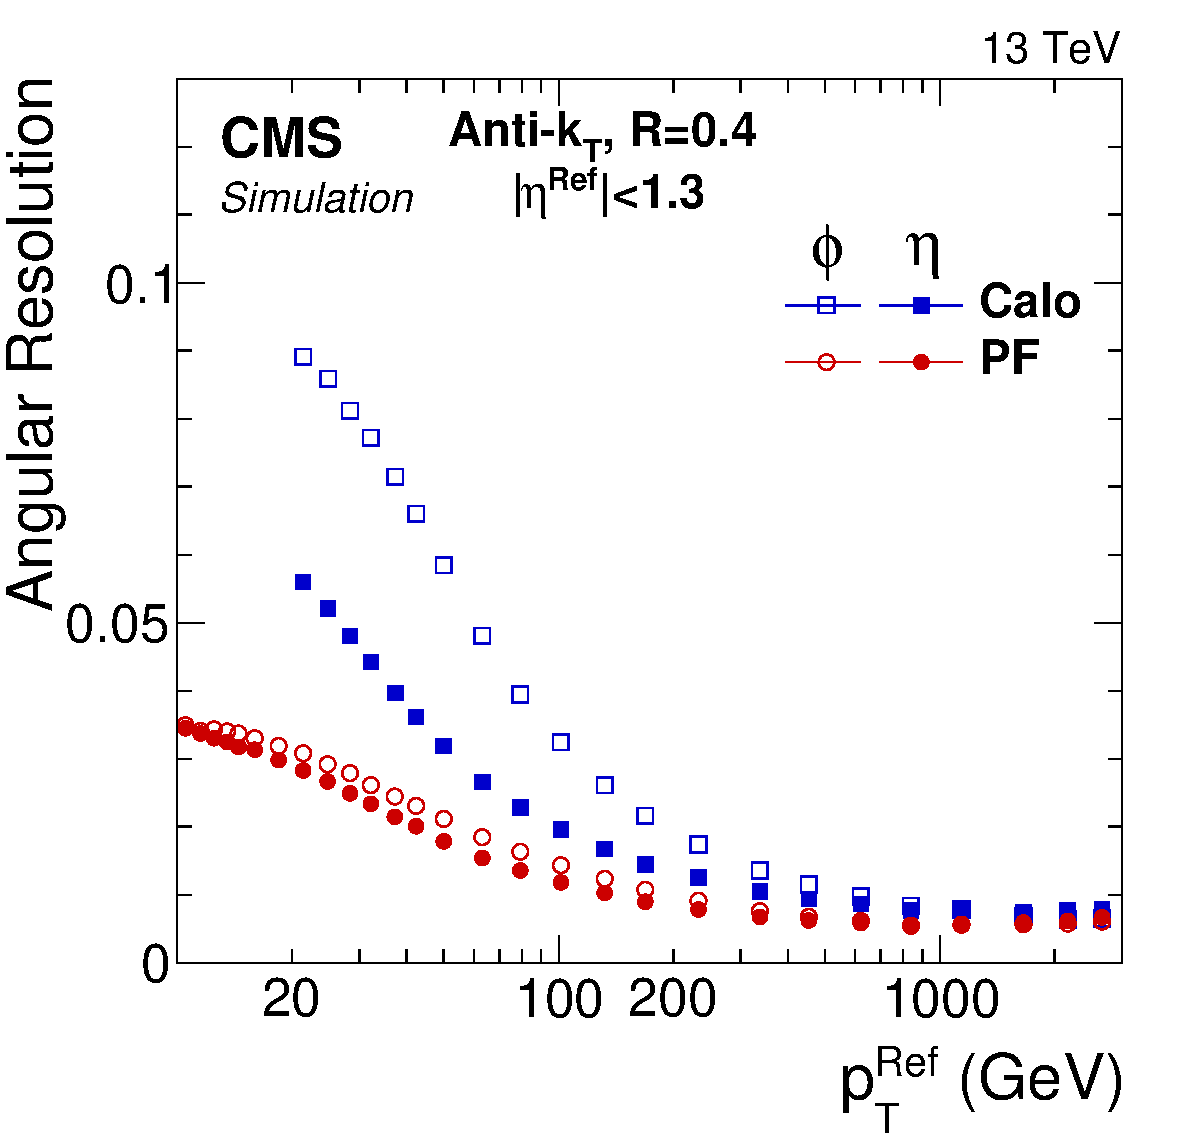
\includegraphics[width=0.45\textwidth]{figs/cms/EtaPhiResVsRefPt_Barrel_AK4CaloL2L3_AK4PFL2L3_RMS_no2000.pdf} 
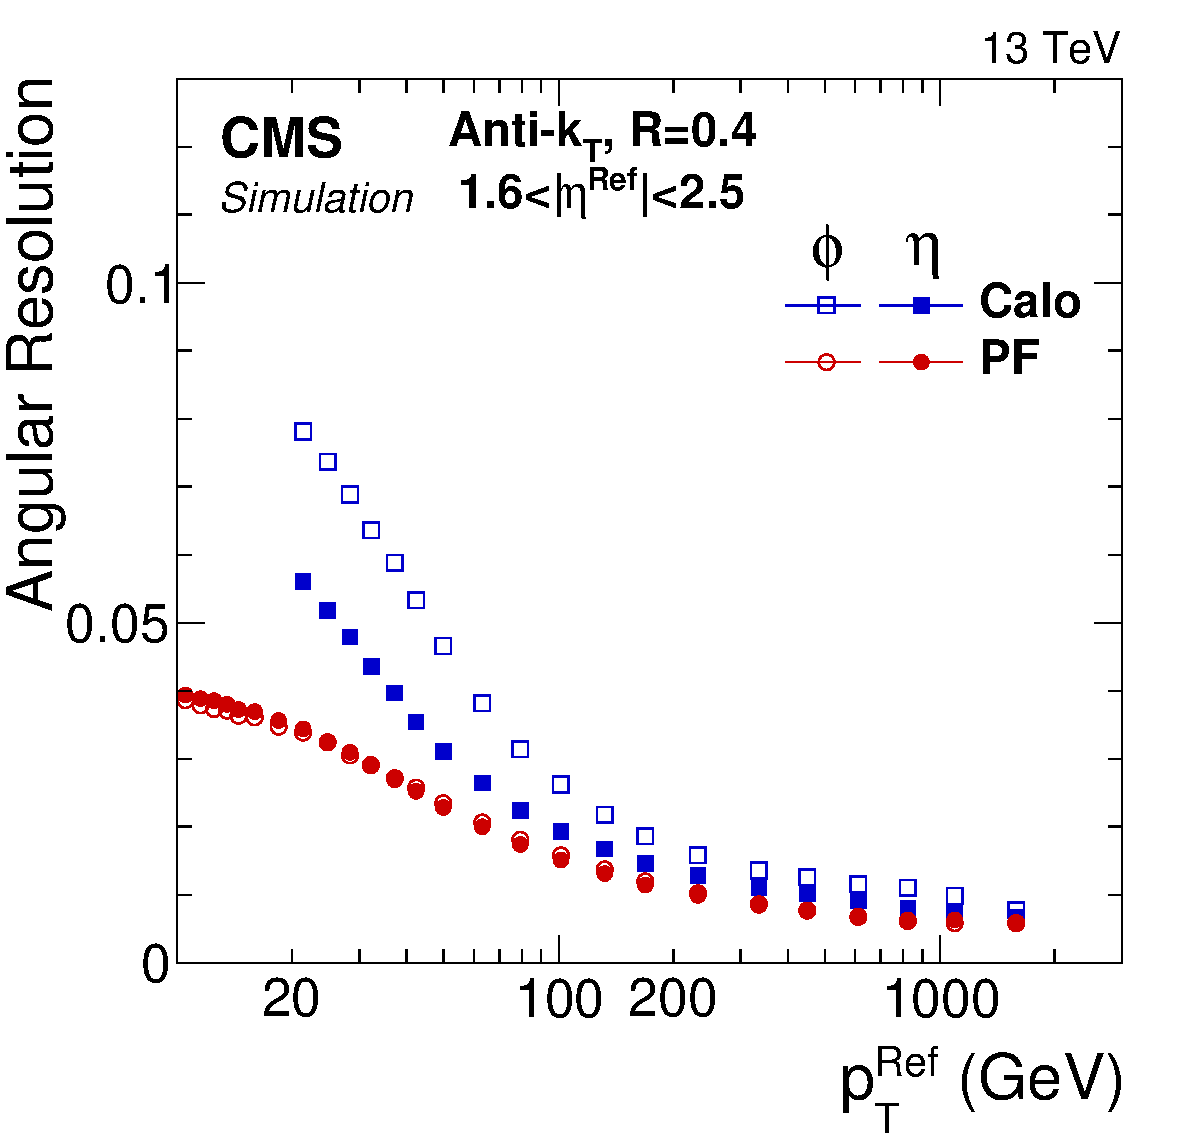
\includegraphics[width=0.45\textwidth]{figs/cms/EtaPhiResVsRefPt_Endcap_AK4CaloL2L3_AK4PFL2L3_RMS_no2000.pdf}
\caption{Jet angular resolution in the barrel (left) and endcap (right) regions, as a function of the transverse momentum of the reference jet.\label{fig:expected_performance_jets_angular}}
\end{figure}


%On average, 65\% of the jet energy is carried by charged hadrons, 25\%
%by photons, and 10\% by neutral hadrons. The ability of the PF
%algorithm to identify these particles in the jets is studied by
%comparing the jet energy fractions measured by the particle flow to
%the ones of the corresponding Ref jet. A significant portion of the
%transverse momentum carried by neutral hadrons is reconstructed as
%photons because the energy deposits of neutral hadrons in the ECAL are
%systematically used to reconstruct photons. Summing up the
%reconstructed energy from photons and neutral hadrons, around 80\% of the neutral hadron energy
%is recovered.

The raw jet energy response, defined as the mean ratio of the
reconstructed jet energy to the reference jet energy, is shown in
Fig.~\ref{fig:expected_performance_jets}. The PF jet response is
linear as a function of the jet transverse momentum and is above 90\%
across the whole detector acceptance. A jet energy correction procedure is used to bring the jet energy
response to unity, removing any dependence on \pt and
$\eta$~\cite{Khachatryan:2016kdb}. After this correction, the jet
energy resolution, defined as the Gaussian width of the ratio between
the corrected and reference jet energies, is also shown in Fig.~\ref{fig:expected_performance_jets}.

\begin{figure}[htbp]
  \centering 
  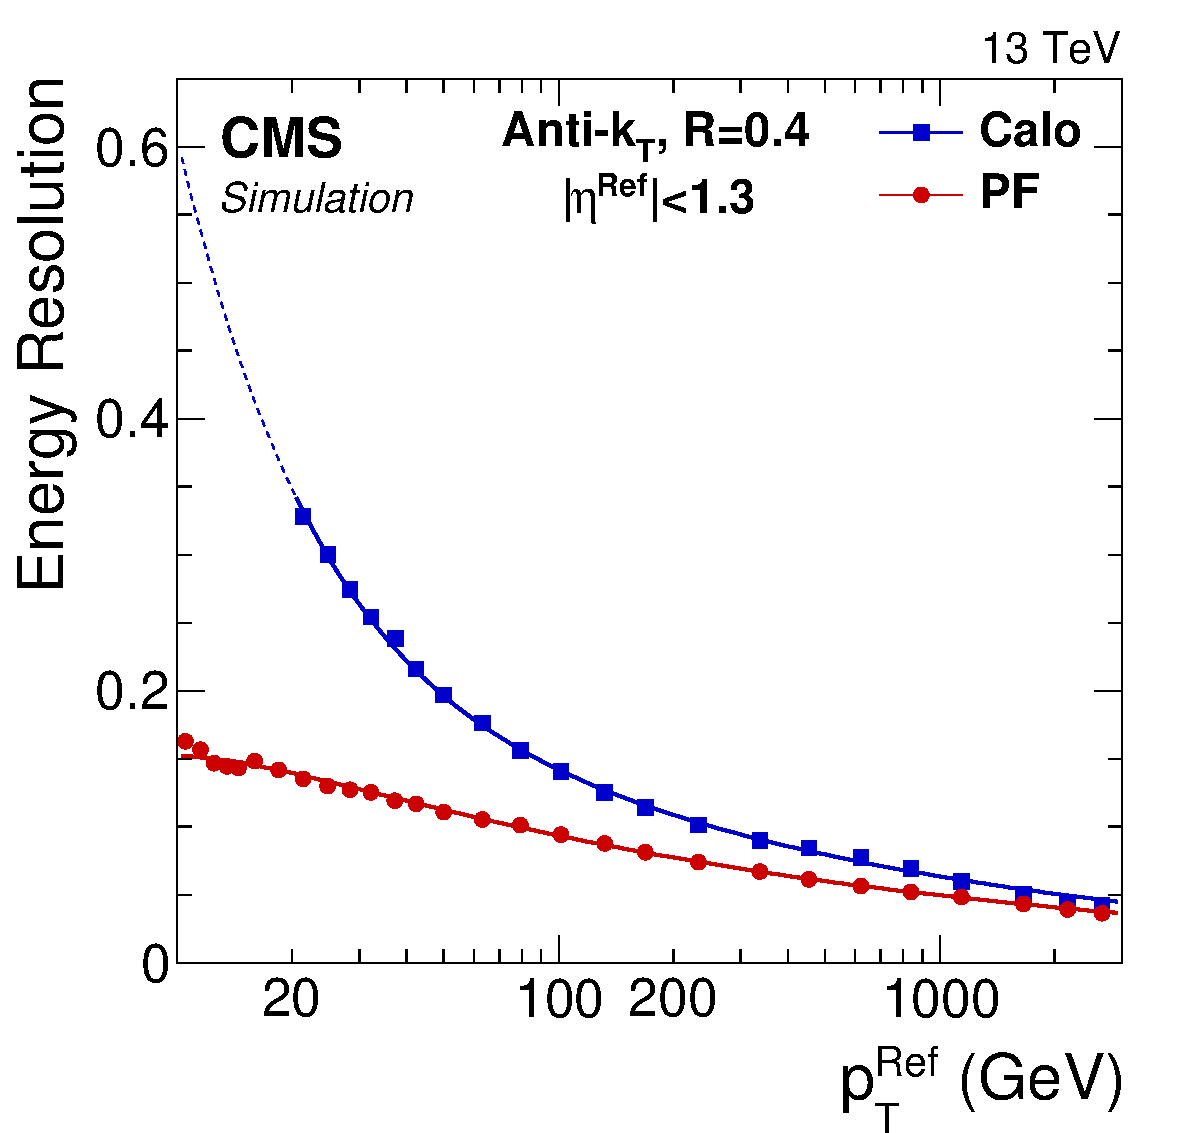
\includegraphics[width=0.45\textwidth]{figs/cms/RelResVsRefPt_Barrel_AK4CaloL2L3_AK4PFL2L3_no2000.pdf}
  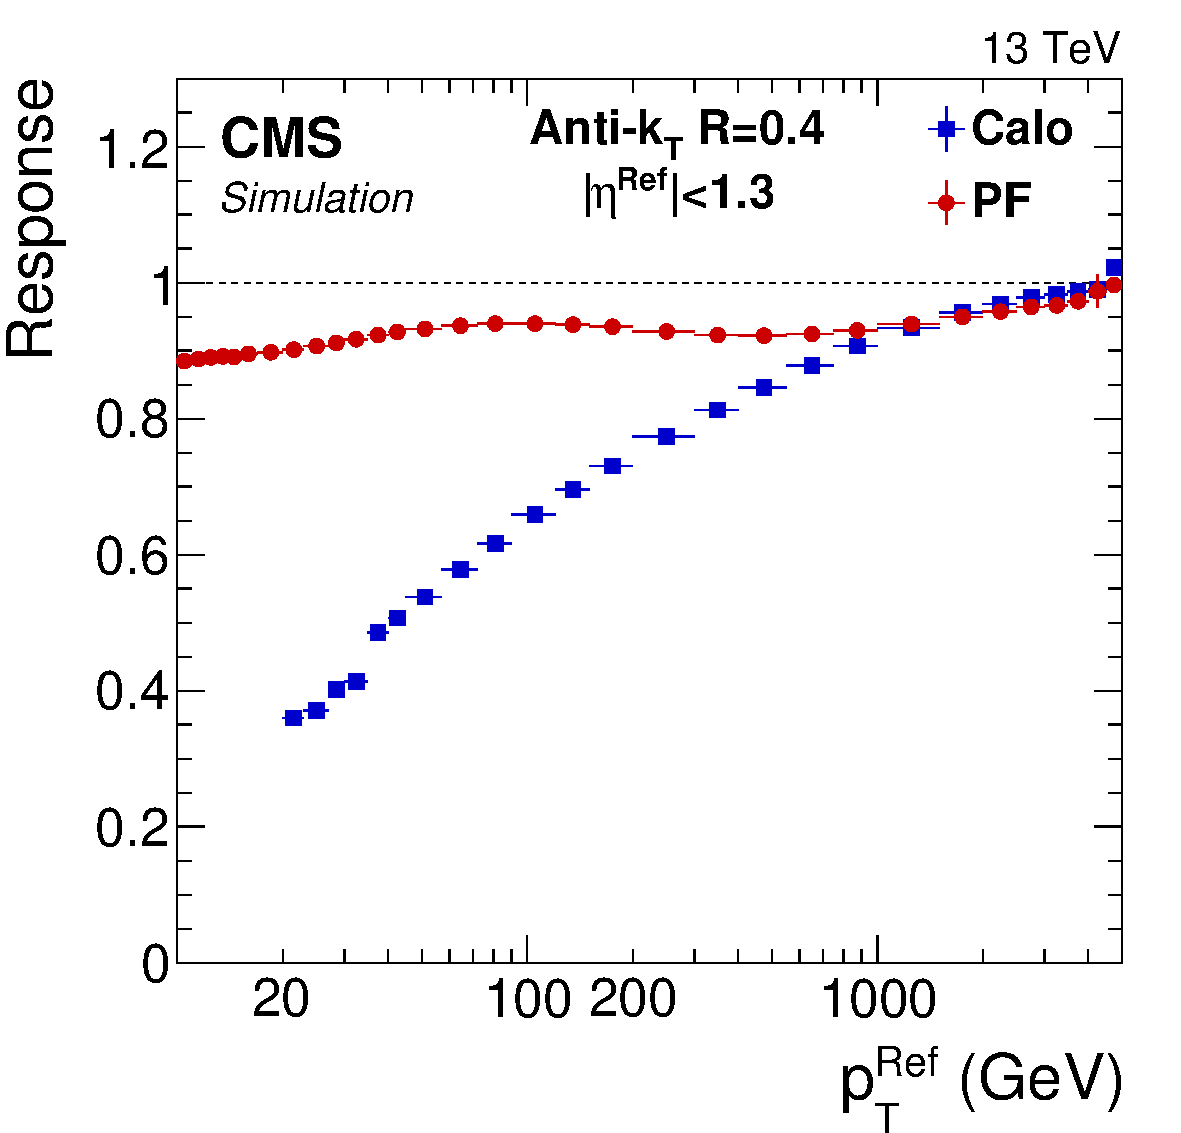
\includegraphics[width=0.45\textwidth]{figs/cms/ClosureRatioVsRefPt_RefEta0to1dot3_ak4caloOverak4pf_no2000.pdf}
  \caption{Jet \pt resolution (left) and jet \pt response (right) as a function of $\pt^{\mathrm{Ref}}$ in the barrel.\label{fig:expected_performance_jets}}
\end{figure}

The presence of particles that do not interact with the detector
material, such as a hypothetical dark matter particle, or simply
neutrinos, is indirectly revealed by missing transverse momentum,
often referred to as missing transverse energy~\cite{Khachatryan:2014gga}. The raw missing transverse momentum
vector is defined in such a way as to balance the vectorial sum of the
transverse momenta of all particles,
\begin{equation}
  \vecptmiss ({\mathrm{PF, raw}}) = - \sum_{i=1}^{N_{\mathrm{particles}}} \vecpt^{\,i}.
\end{equation}
The jet-energy-corrected missing transverse momentum,
\begin{equation}
  \vecptmiss ({\mathrm{PF}}) = - \sum_{i=1}^{N_{\mathrm{particles}}}
  \vecpt^{\,i} - \sum_{j=1}^{N_{\mathrm{PF\,jets}}} ({\vec p^{\,\mathrm{corr}\,j}_{\mathrm T}} - \vecpt^{\,j})~,
\end{equation}
includes a jet energy correction term that replaces the raw momentum
$\vecpt^{\,j}$  of each PF jet with $\vecpt^{\,j} >10\,\GeV$ by its
corrected value $\vec p^{\,\mathrm{corr}\,j}_{{\mathrm T}}$.
As seen in Fig.~\ref{fig:expected_performance_jets}, the
PF jet response is close to unity, making this correction term small
when the missing transverse energy is evaluated with reconstructed
particles.

Before the advent of PF reconstruction, the missing transverse
momentum was evaluated using information from the calorimeters and the
muon system as,
\begin{equation}
  \vecptmiss ({\mathrm{Calo}}) = - \sum_{i=1}^{N_{\mathrm{cells}}}
  \vecpt^{\,i} - \sum_{j=1}^{N_{\mathrm{Calo\,jets}}} ({\vec p^{\,\mathrm{corr}\,j}_{\mathrm T}} - \vecpt^{\,j}) - \sum_{k=1}^{N_{\mathrm{muons}}} \vecpt^{\,k}~,
\end{equation}
where in the first term, the transverse momentum $\vecpt^{\,i}$ of a
given calorimeter cell is calculated assuming that the energy
measured by the cell has been deposited by a massless particle coming
from the origin. The jet energy correction term, computed with all
Calo jets with $\pt>20\,\GeV$, is sizeable given the relatively low energy response
of Calo jets. The second correction term accounts for the presence of
identified muons, which do not deposit significant energy in the calorimeters.

The performance improvement due to PF reconstruction may be
quantified by comparing $\vecptmiss(\mathrm{PF})$ and
$\vecptmiss(\mathrm{Calo})$ in terms of \MET response and
resolution. The \MET resolution is measured for a simulated QCD
multijet sample of events in Fig~\ref{fig:expected_performance_met} as a function of $\sumET$, the total
transverse energy developed in the event. Since the vast majority of
QCD multijet events have no true \MET, the distribution of the
transverse components of the \vecMET, $\vecMETxy$, can be approximated
as a Gaussian\footnote{Typically non-Gaussian tails emerge due to
  non-Gaussian response functions of the detector.} centered at zero
and its width provides an estimate of the \MET resolution as $\sigma(\MET)=\sqrt{2} \times
\sigma(\METxy)$. The \sumET response, defined as the average fraction of the true \sumET to
be reconstructed, is also shown in Fig~\ref{fig:expected_performance_met}. Finally, the \vecMET
angular resolution, measured for a sample of \ttbar events in which at
least one neutrino is produced in the decay of a $\PW$ boson, is shown
in Fig.~\ref{fig:expected_performance_met_phi_resolution}.  As in
the case of jets, the superior response and resolution mainly arises
from the improved measurement of the momenta of charged hadrons.


\begin{figure}[htbp]
\centering
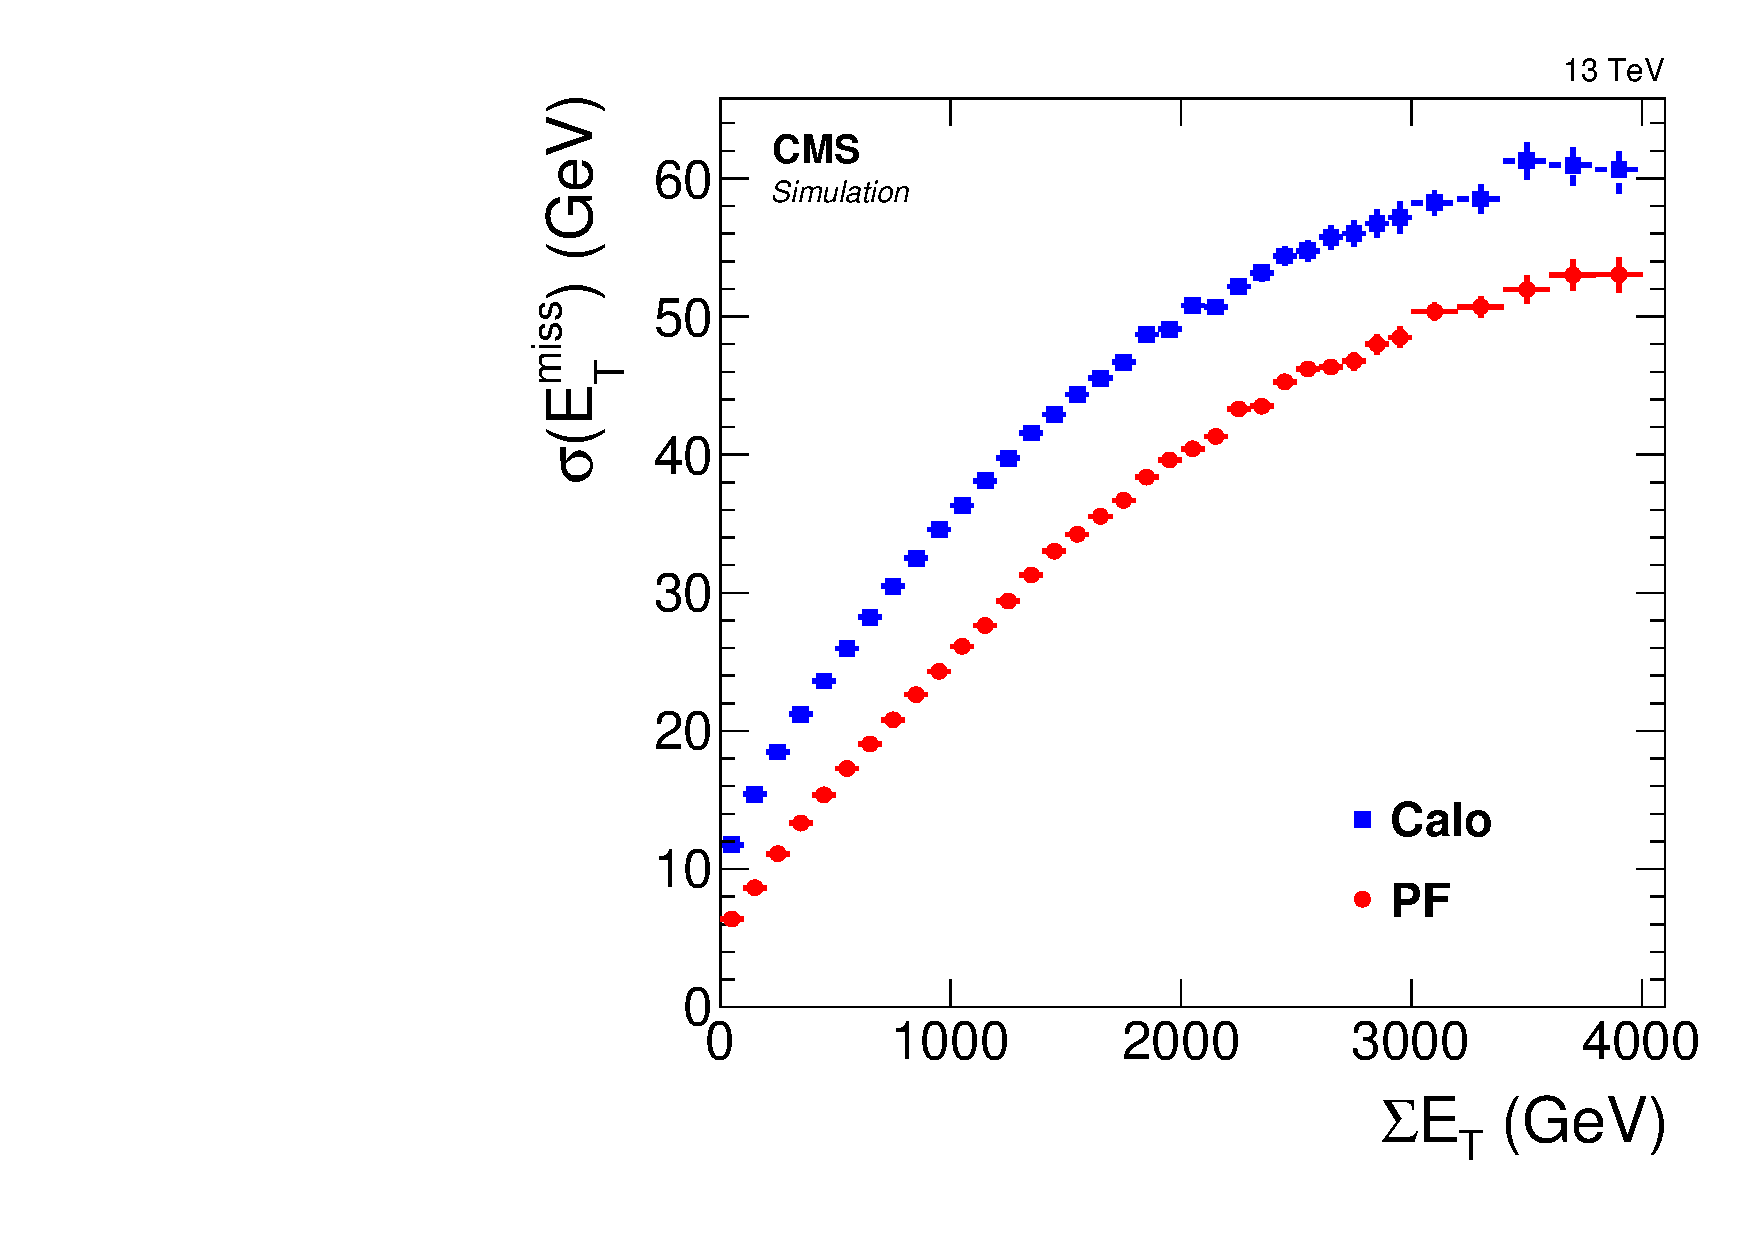
\includegraphics[width=0.45\textwidth]{figs/cms/met_sigma_vs_sumet.pdf}
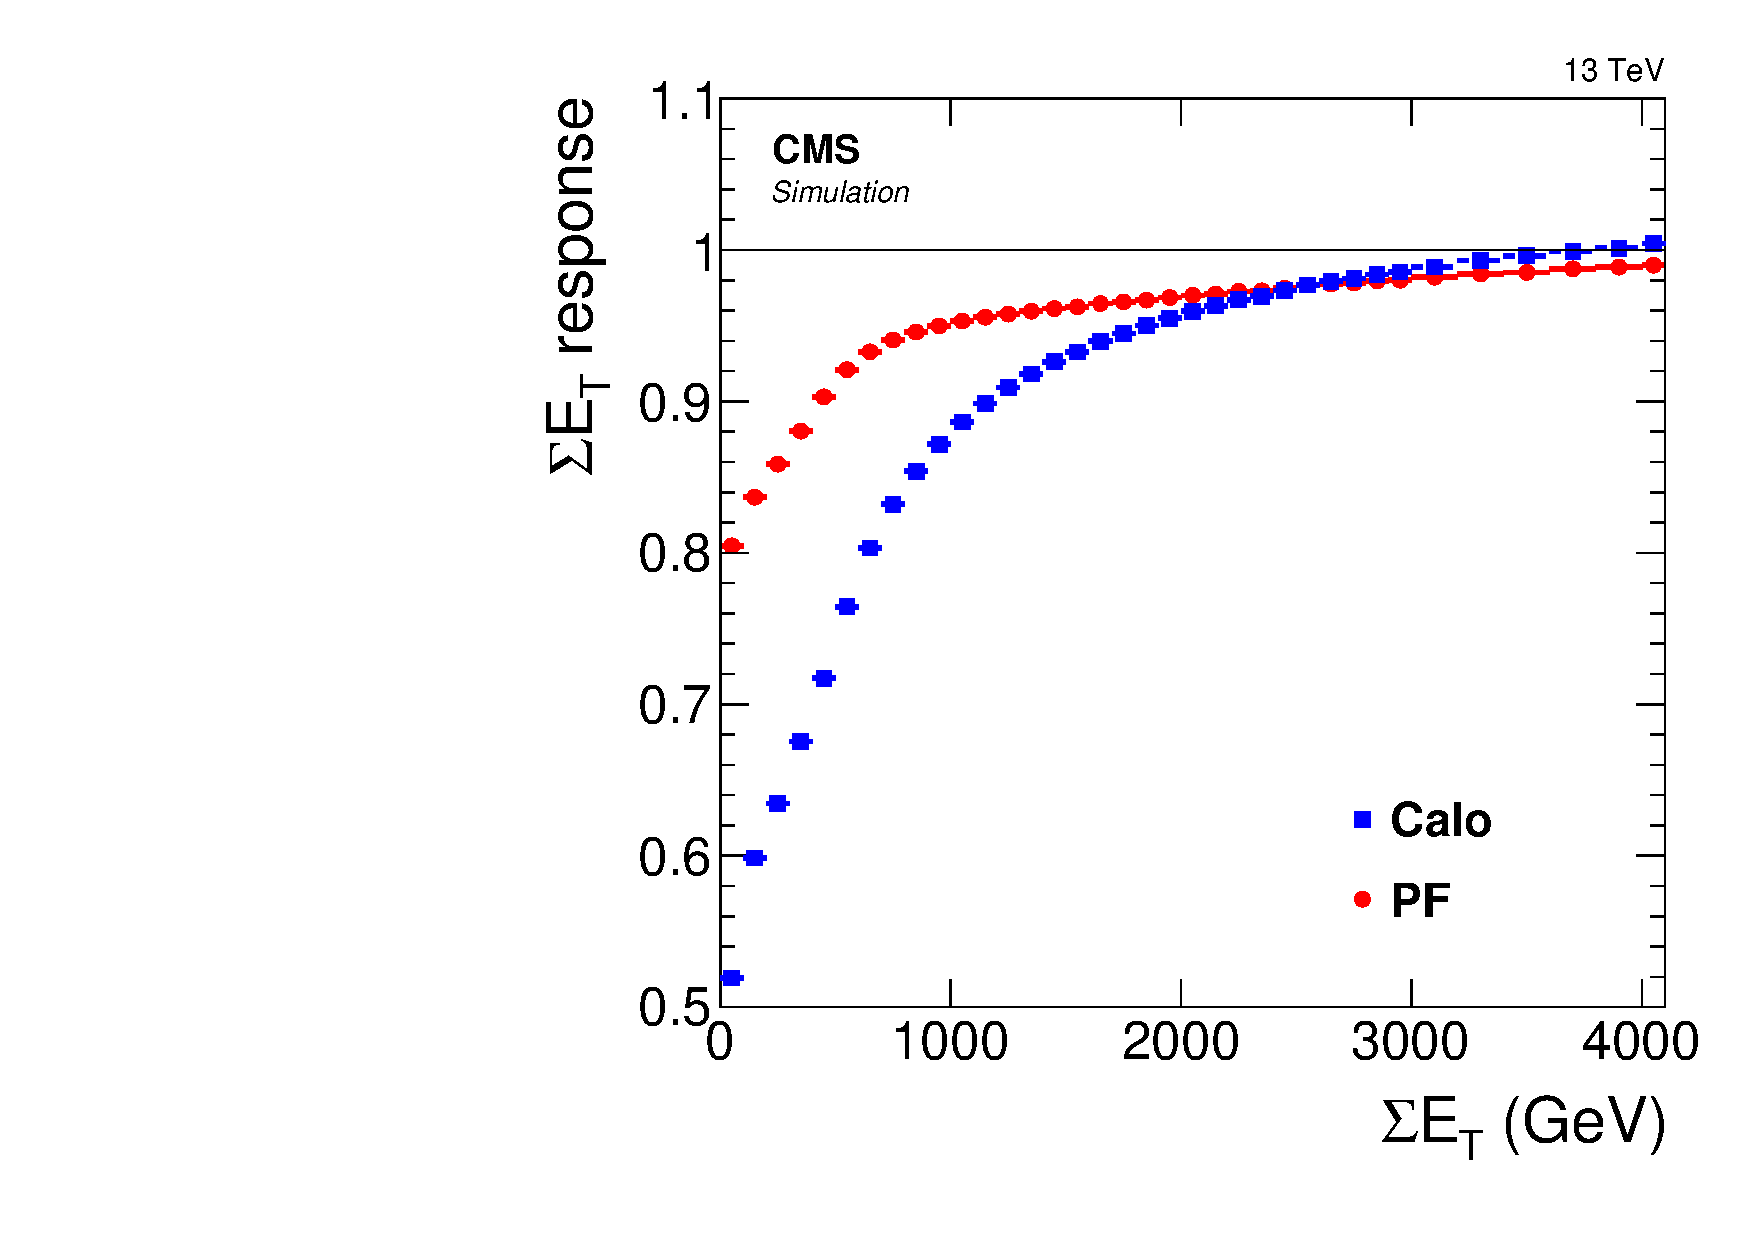
\includegraphics[width=0.45\textwidth]{figs/cms/met_response_vs_sumet.pdf}
\caption{Absolute \MET resolution (left) and \sumET response (right) for a simulated QCD multijet sample.
In the case of the particle flow estimate, \MET stands for $\MET ({\mathrm{PF}})$ and \sumET for $\sumET ({\mathrm{PF}})$. In the case of the calorimeter-based estimate, they stand for $\MET ({\mathrm{Calo}})$ and $\sumET ({\mathrm{Calo}})$.\label{fig:expected_performance_met}}
\end{figure}

\begin{figure}[htbp]
\centering
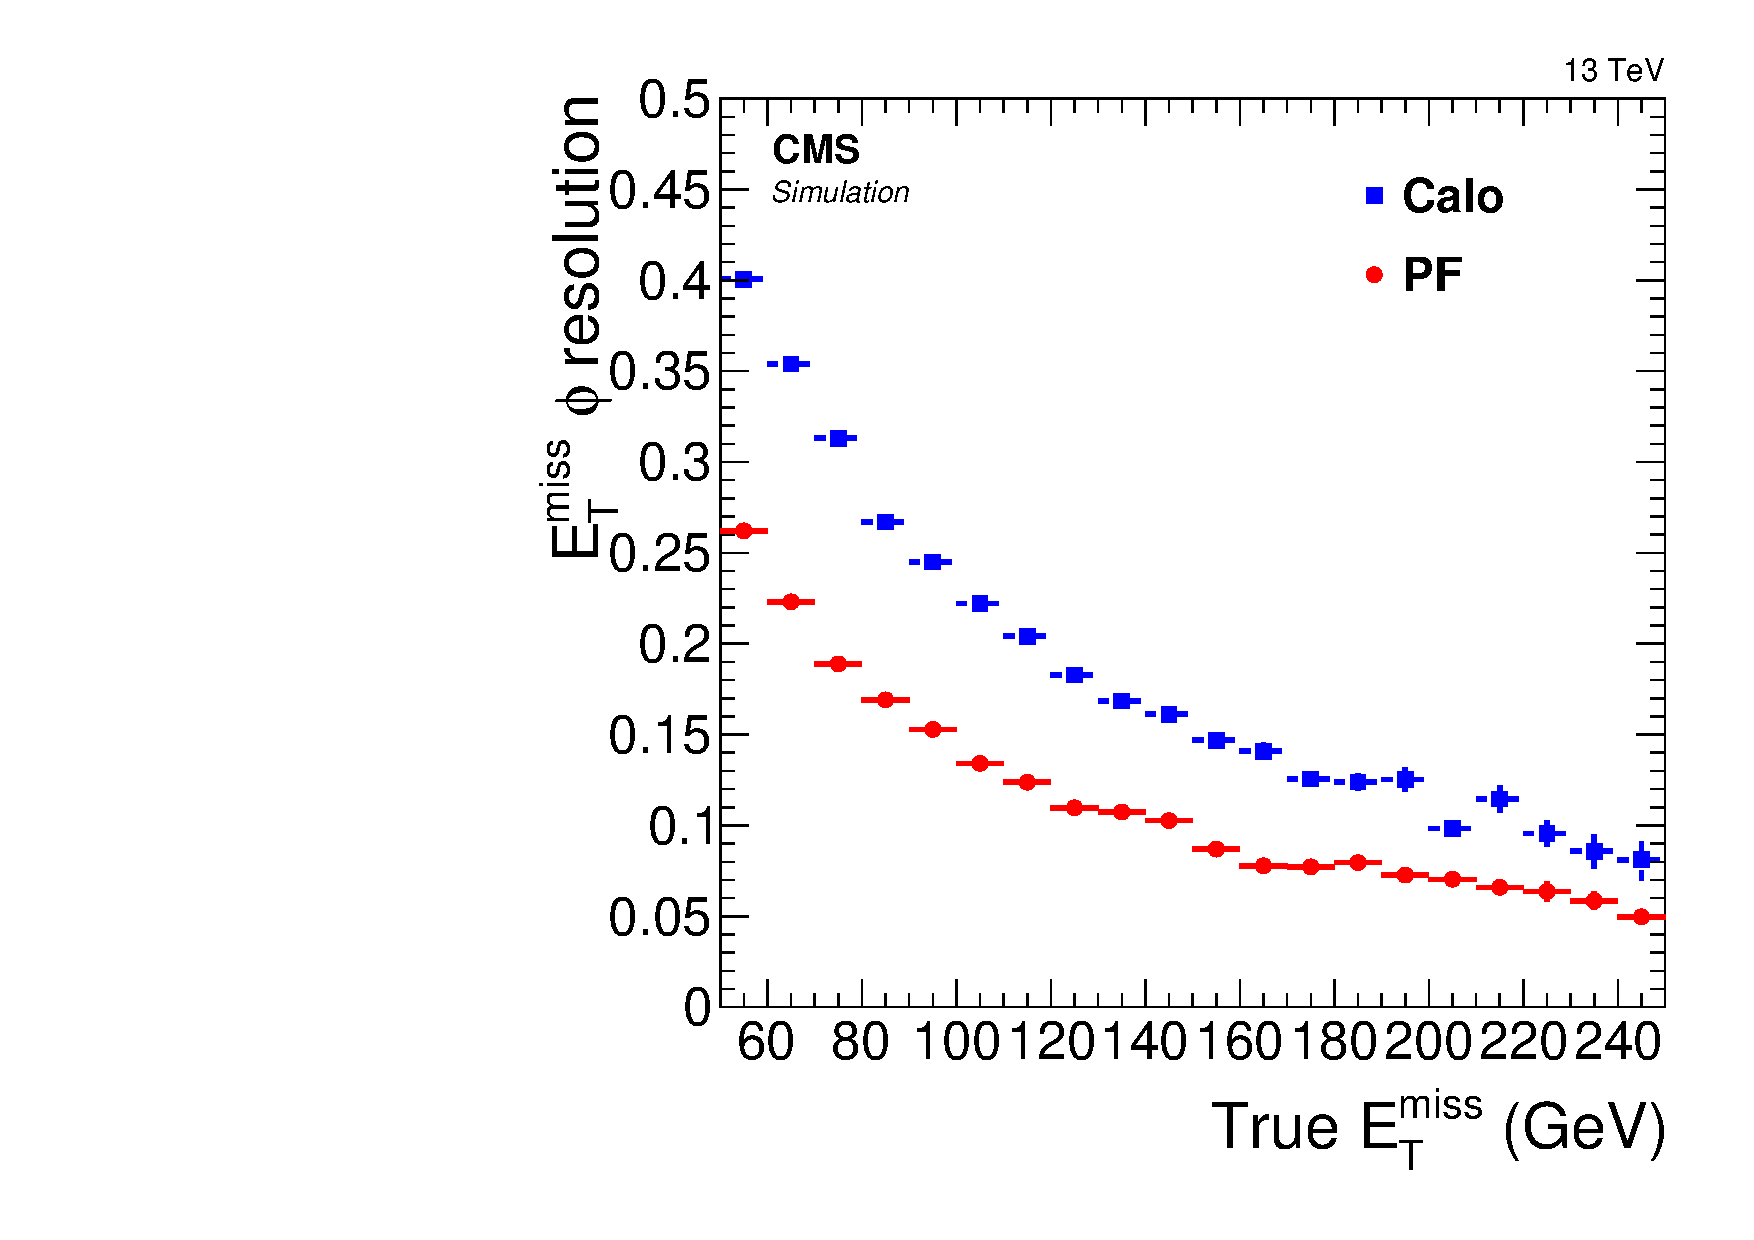
\includegraphics[width=0.49\textwidth]{figs/cms/met_phi_vs_truemet.pdf}
\caption{
Resolution on the measurement of the \vecMET azimuthal angle as a function of the true \MET for a simulated \ttbar sample.
\label{fig:expected_performance_met_phi_resolution}}
\end{figure}

Rare failures related to the detector, the reconstruction of the PF inputs, 
and the algorithm itself generally translate to unexpectedly large values of the \MET.
Events with such large values are systematically scrutinized and when a shortcoming of the PF algorithm is fixed, 
the global performance of the PF reconstruction typically improves as a whole population of events were affected at lower values
of the \MET. 

The performance of \VEtmiss reconstruction with all corrections
applied is assessed with a sample
of observed events selected in the dimuon final state that is
dominated by events with a $\cPZ$ boson decaying to two
muons~\cite{Khachatryan:2014gga}. The dataset is collected with a
trigger requiring the presence of two muons passing \pt thresholds of
17 and 8\GeV, respectively. The two reconstructed muons must fulfill $\pt > 20 $\GeV and $|\eta| <
2.1$, satisfy isolation requirements, and have opposite charge. Events where the invariant mass of the dimuon system is outside the
window $60<m_{\mu\mu}<120$\GeV are rejected.
%The expression of $\vecMET (\mathrm{PF})$, defined above, includes a
%correction term accounting for the response of the jets in the final
%state. Here, two additional terms are introduced, the first to correct
%for the presence of many low-energy particles from pileup
%interactions, and a second one to correct for an observed $\Phi$
%asymmetry due to a shift in $\vecMET (\mathrm{PF})$ along the detector
%$x$ and $y$ axes.
Figure~\ref{fig:met_distribution} shows the spectrum
of $\MET ({\mathrm{PF}})$ in the $\cPZ\rightarrow\mu\mu$ event sample. The
simulation describes the observed distribution over more than five
orders of magnitude.

\begin{figure}[htp]\centering
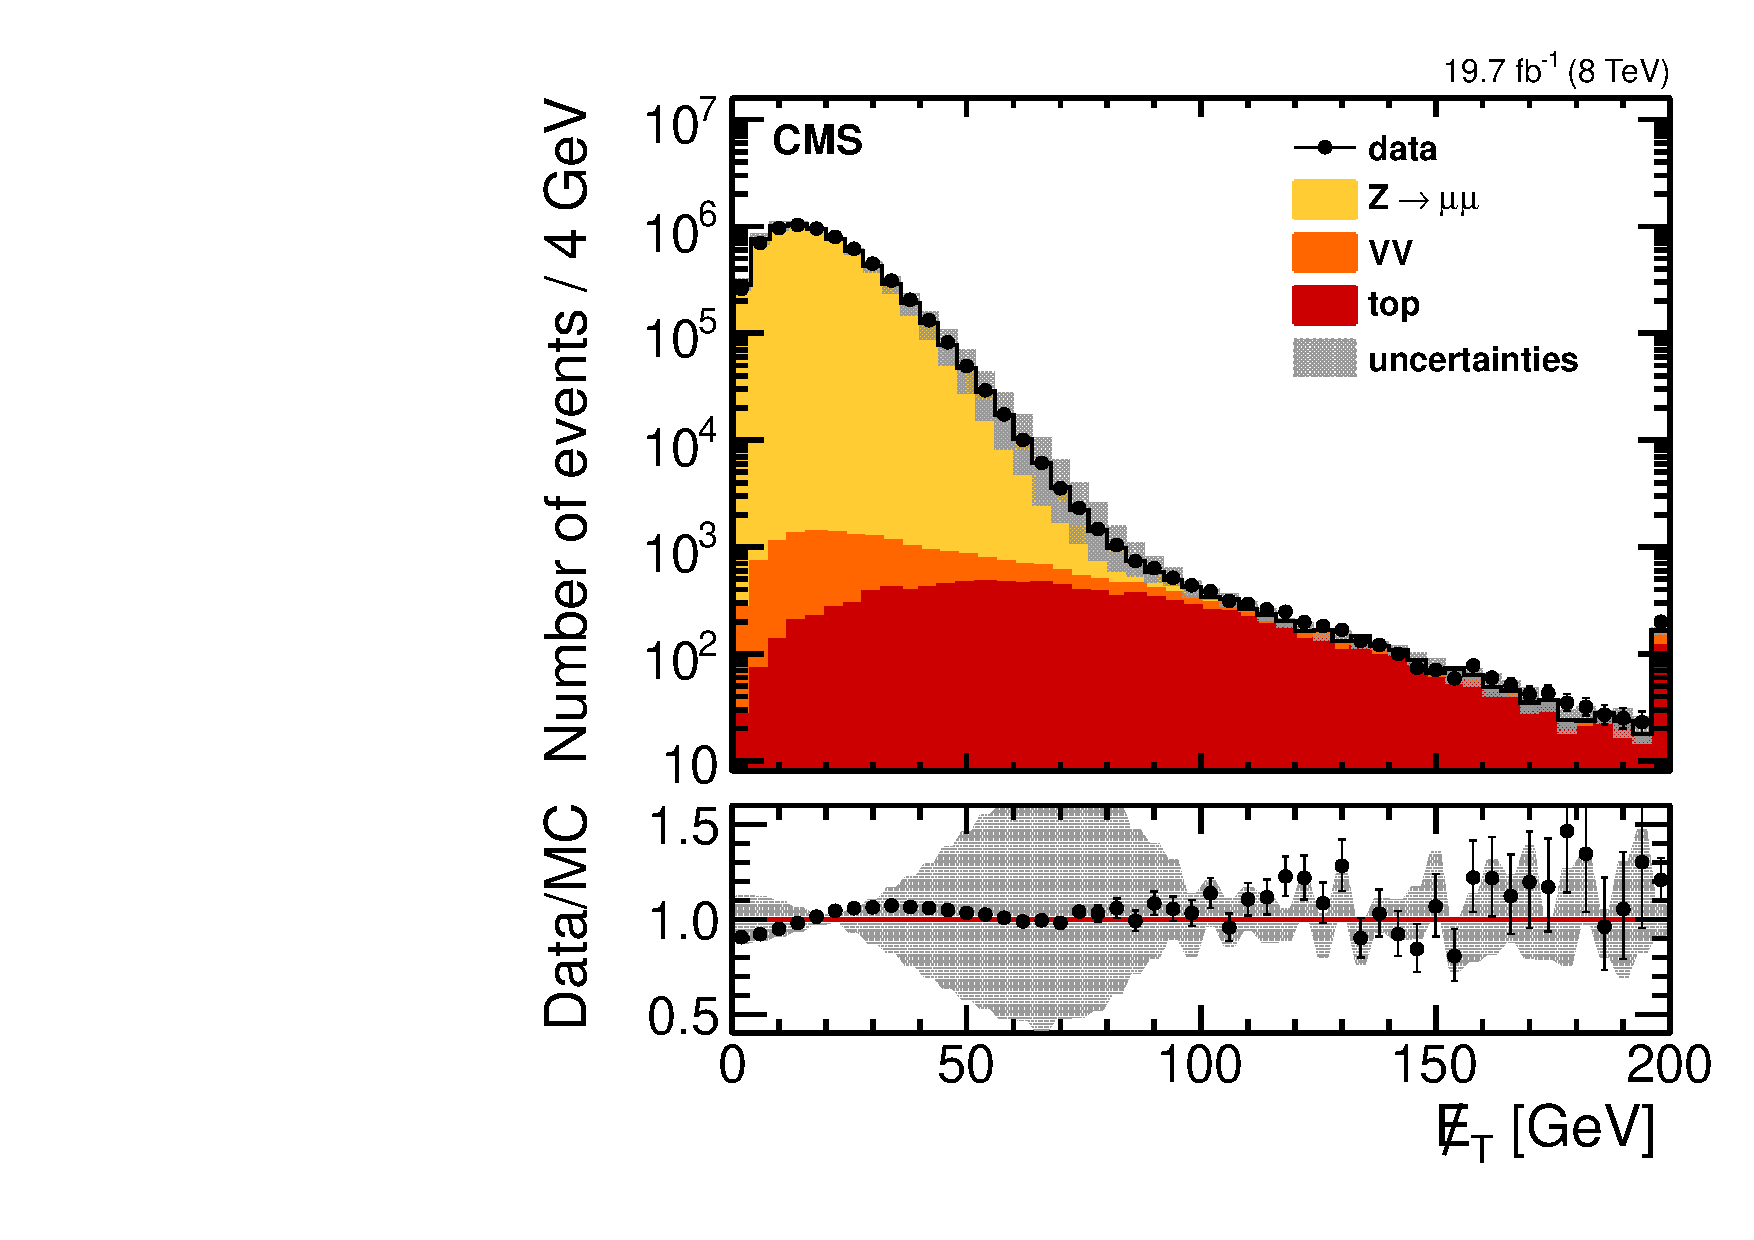
\includegraphics[width=.7\linewidth]{figs/cms/pFlowPFMET.pdf}
\caption{Spectrum of $\MET (\mathrm{PF})$ in the $\cPZ\rightarrow\mu\mu$ dataset.
The observed data are compared to simulated $\cPZ\rightarrow\mu\mu$,
diboson (VV), and $\ttbar$ plus single-top-quark events (top).
The lower frame shows the ratio of data to simulation, with the
uncertainty bars of the points including the statistical uncertainties
of both observed and simulated events and the grey uncertainty band
displaying the systematic uncertainty of the simulation. The last bin contains the overflow.\label{fig:met_distribution}}
\end{figure}

\subsection{Identification of \PQb-quark Jets}
\label{sec:btag}
Jets that arise from bottom-quark hadronization (\cPqb-jets) are
present in many physics processes, such as the decay of top quarks,
the Higgs boson, and top and bottom squarks predicted by natural supersymmetric models. 
The ability to accurately identify \cPqb-jets is crucial in reducing
the otherwise overwhelming background from processes
involving jets from gluons (\cPg), light-flavor quarks (\cPqu,
\cPqd, \cPqs), and from \cPqc-quark fragmentation. 

The properties of the bottom and, to a lesser extent, the charm
hadrons can be used to identify the hadronic jets into which the
\cPqb\ and \cPqc\ quarks fragment.  These hadrons have relatively
large masses, long lifetimes ($c\tau\sim 450~\mu\mathrm{m}$) and daughter particles with hard momentum
spectra. Their semileptonic decays can be exploited as well.


Within the CMS collaboration, these special features of \cPqb-quark
hadronization are exploited in a set of \cPqb-jet tagging algorithms. A variety of reconstructed objects -- tracks, vertices and identified
leptons -- can be used to build observables that discriminate between
\Pqb- and light-parton jets. Several simple and robust algorithms use
just a single observable, while others combine several of these
objects to achieve a higher discrimination power. Each of these
algorithms yields a single discriminator value for each jet. The
minimum thresholds on these discriminators define loose (``L''), medium
(``M''), and tight (``T'') operating points with a misidentification
probability for light-parton jets of close to 10\%, 1\%, and 0.1\%,
respectively, at an average jet \pt of about $80 \GeV$.

The \cPqb-tag algorithm that was shown to have the best performance
in terms of \cPqb-jet identification efficiency and light-parton-jet fake rate
in Run 1 is the \emph{Combined Secondary Vertex} (CSV)
algorithm, which makes use of multivariate techniques to combine
discriminating variables built from displaced track and secondary
vertex information as well as jet
kinematics~\cite{btag7TeV,btag8TeV}. The following set of
variables with high discriminating power and low correlations is used:
\begin{itemize}
\item the vertex category (real, ``pseudo,'' or ``no vertex'');
\item the flight distance significance (ratio of the flight
  distance to its estimated uncertainty) in the transverse plane (``2D'');
\item the vertex mass;
\item the number of tracks at the vertex;
\item the ratio of the energy carried by tracks at the vertex with respect to all tracks in the jet;
\item the pseudorapidities of the tracks at the vertex with respect to the jet axis;
\item the 2D impact parameter (IP) significance (ratio of the IP to its estimated uncertainty, ) of the first track that raises the invariant mass above the charm threshold of $1.5 \GeV$ (tracks are ordered by decreasing IP significance and the mass of the system is recalculated after adding each track);
\item the number of tracks in the jet;
\item the 3D IP significances for each track in the jet.
\end{itemize}
If no secondary vertex is reconstructed, only the last two variables
in the preceding list are available. Two likelihood ratios are built from these variables to
discriminate between \cPqb-  and \cPqc-jets and between \cPqb\ and
light-parton jets. They are combined with prior weights of $0.25$ and $0.75$, respectively.

The \cPqb-jet identification
efficiency is about 70\% for a misidentification probability for
light-parton jets of about 1\% for jets with \pt between $80$ and $120 \GeV$,
as seen in Fig.~\ref{fig:mcPerformance}.
For Run 2, the CSV algorithm was significantly improved (CSVv2) by
updating the multivariate algorithm from a simple likelihood
ratio to a neural network, improving the track selection and
adding new variables, and using a new algorithm for the
reconstruction of the secondary vertices, the so-called Inclusive
Vertex Finder (IVF).  These updates turn into a net improvement in
performance of about a 10\% increase in the \cPqb-jet identification
efficiency at a 1\% of light-parton-jet misidentification rate, as pictured
in Fig.~\ref{fig:mcPerformance2015}. The \cPqb-jet identification at
HLT uses the same algorithm as in the offline reconstruction, optimized to reduce the execution time~\cite{Tosi:2015zhy}. 
%This was achieved thanks to a more extensive use of the Iterative Tracking reconstruction in the regions-of-interest, which helps in reducing the combinatorics. The second goal is to improve the performance of the online version of the b-tagging algorithm. This was achieved thanks to the Iterative Tracking reconstruction, to the new implementation of the b-tagging algorithm (CSVv2+IVF) and to a better resolution on the position of the primary vertex. By using tracks from the Iterative Tracking, and performing the vertex fitting with an Adaptive Vertex Fitter [6] where the track clustering is made with a Deterministic Annealing (DA) algorithm [7], indeed, the resolution on the position of the primary vertex along the z-axis is about 20-30 μm.

\begin{figure}
\centering
\subfigure{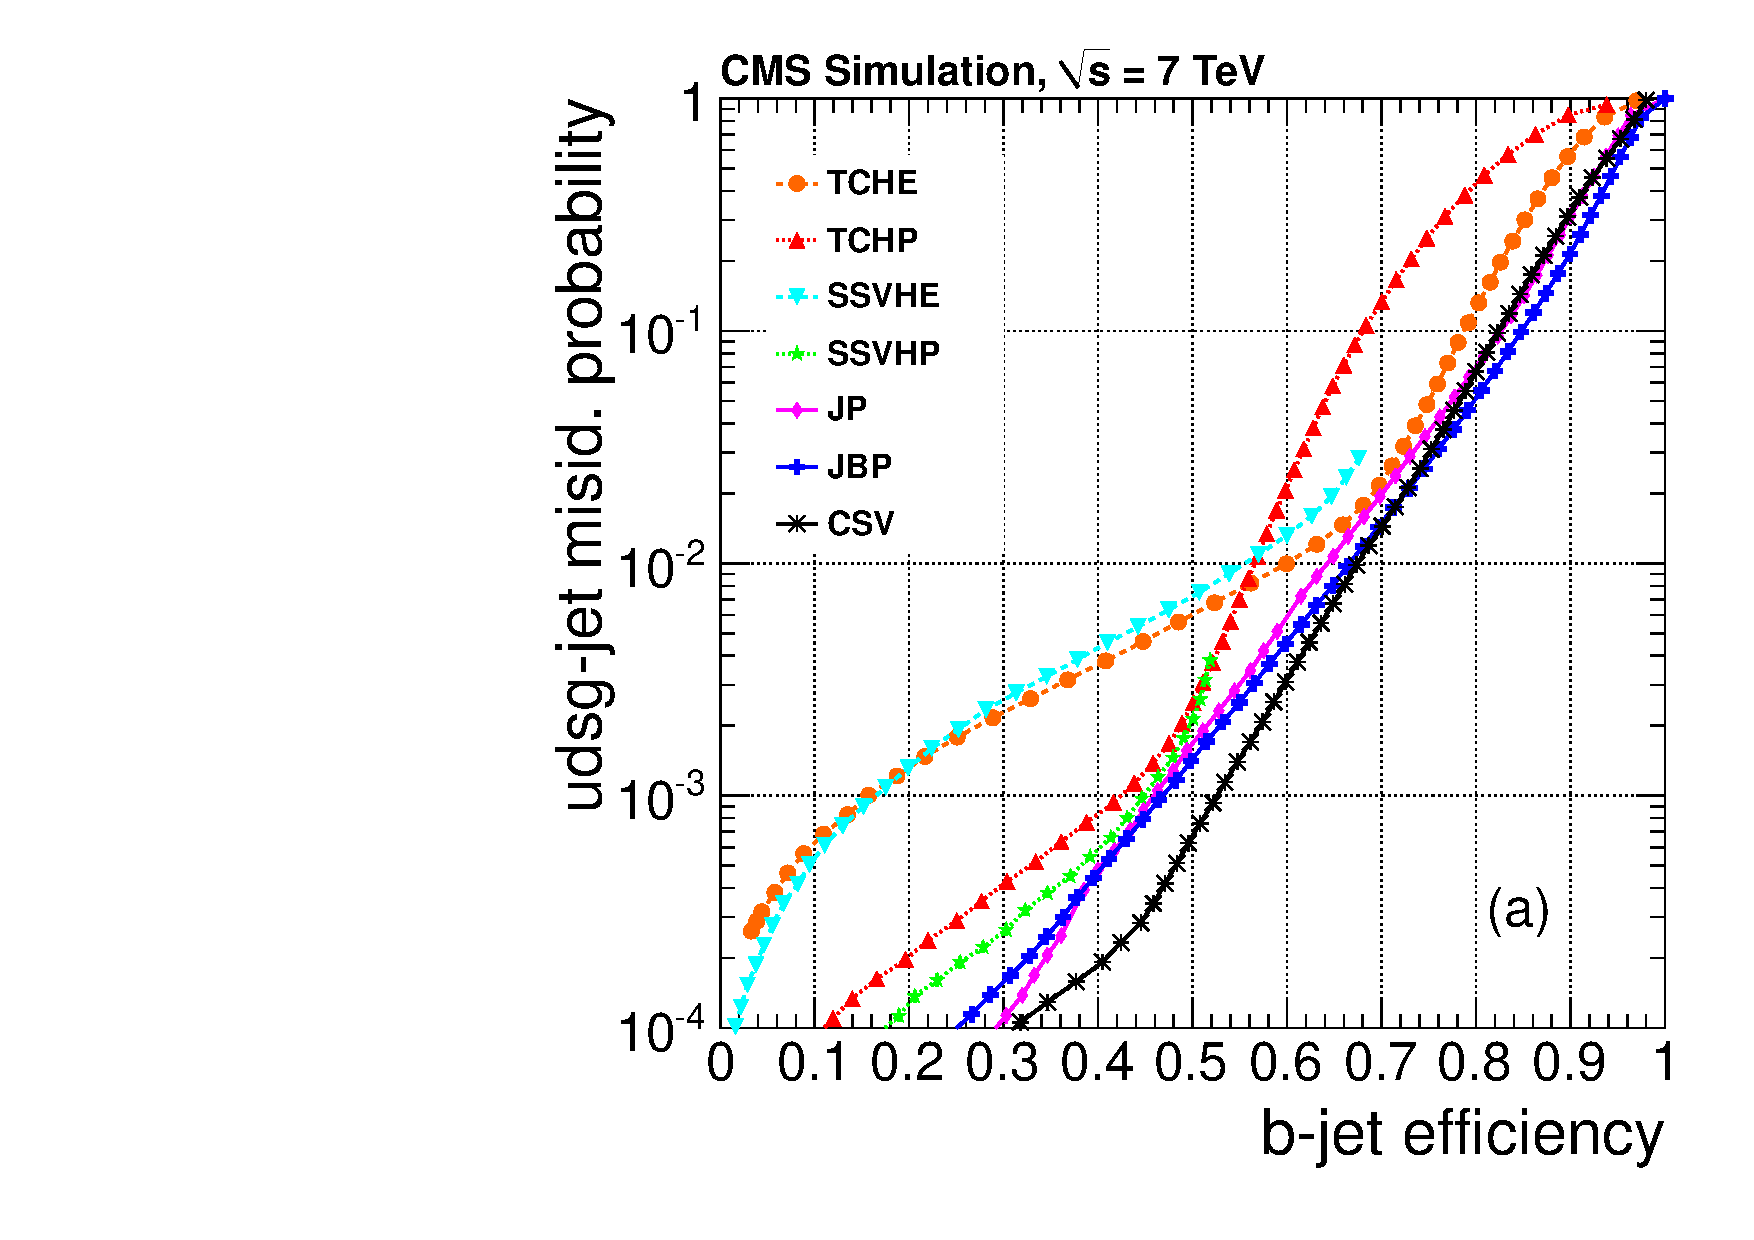
\includegraphics[width=0.45\textwidth]{figs/cms/Combined_udsgvsb_Efficienies.pdf}}
\subfigure{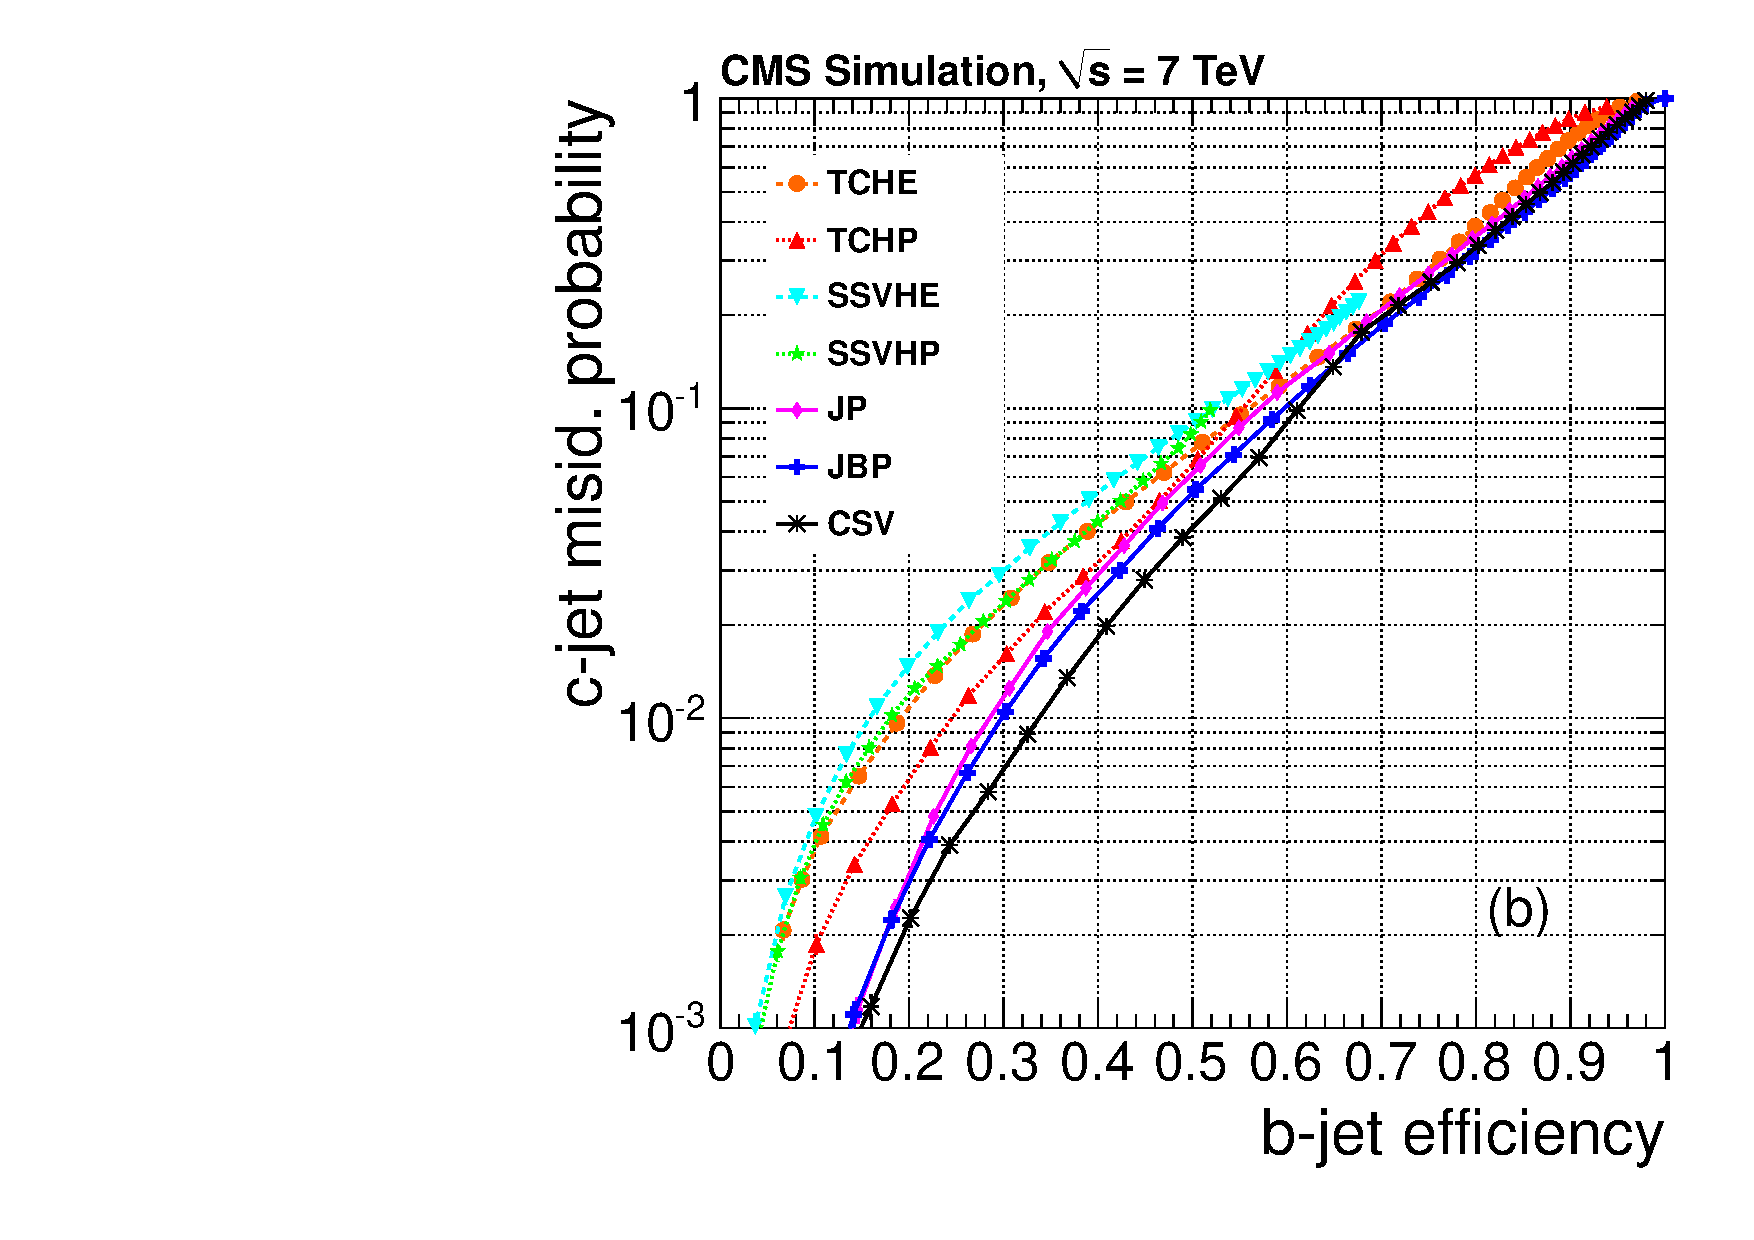
\includegraphics[width=0.45\textwidth]{figs/cms/Combined_cvsb_Efficienies.pdf}}
\caption{
Performance curves obtained from simulation for the different
\cPqb-jet tagging algorithms. Light-parton- (left) and \cPqc-jet (right) misidentification probabilities as a function of the \cPqb-jet efficiency.  Jets with $\pt > 60\GeV$ in a sample of simulated multijet events are used to obtain the efficiency and misidentification probability values.
\label{fig:mcPerformance}}
\end{figure}

\begin{figure}
\centering
\subfigure{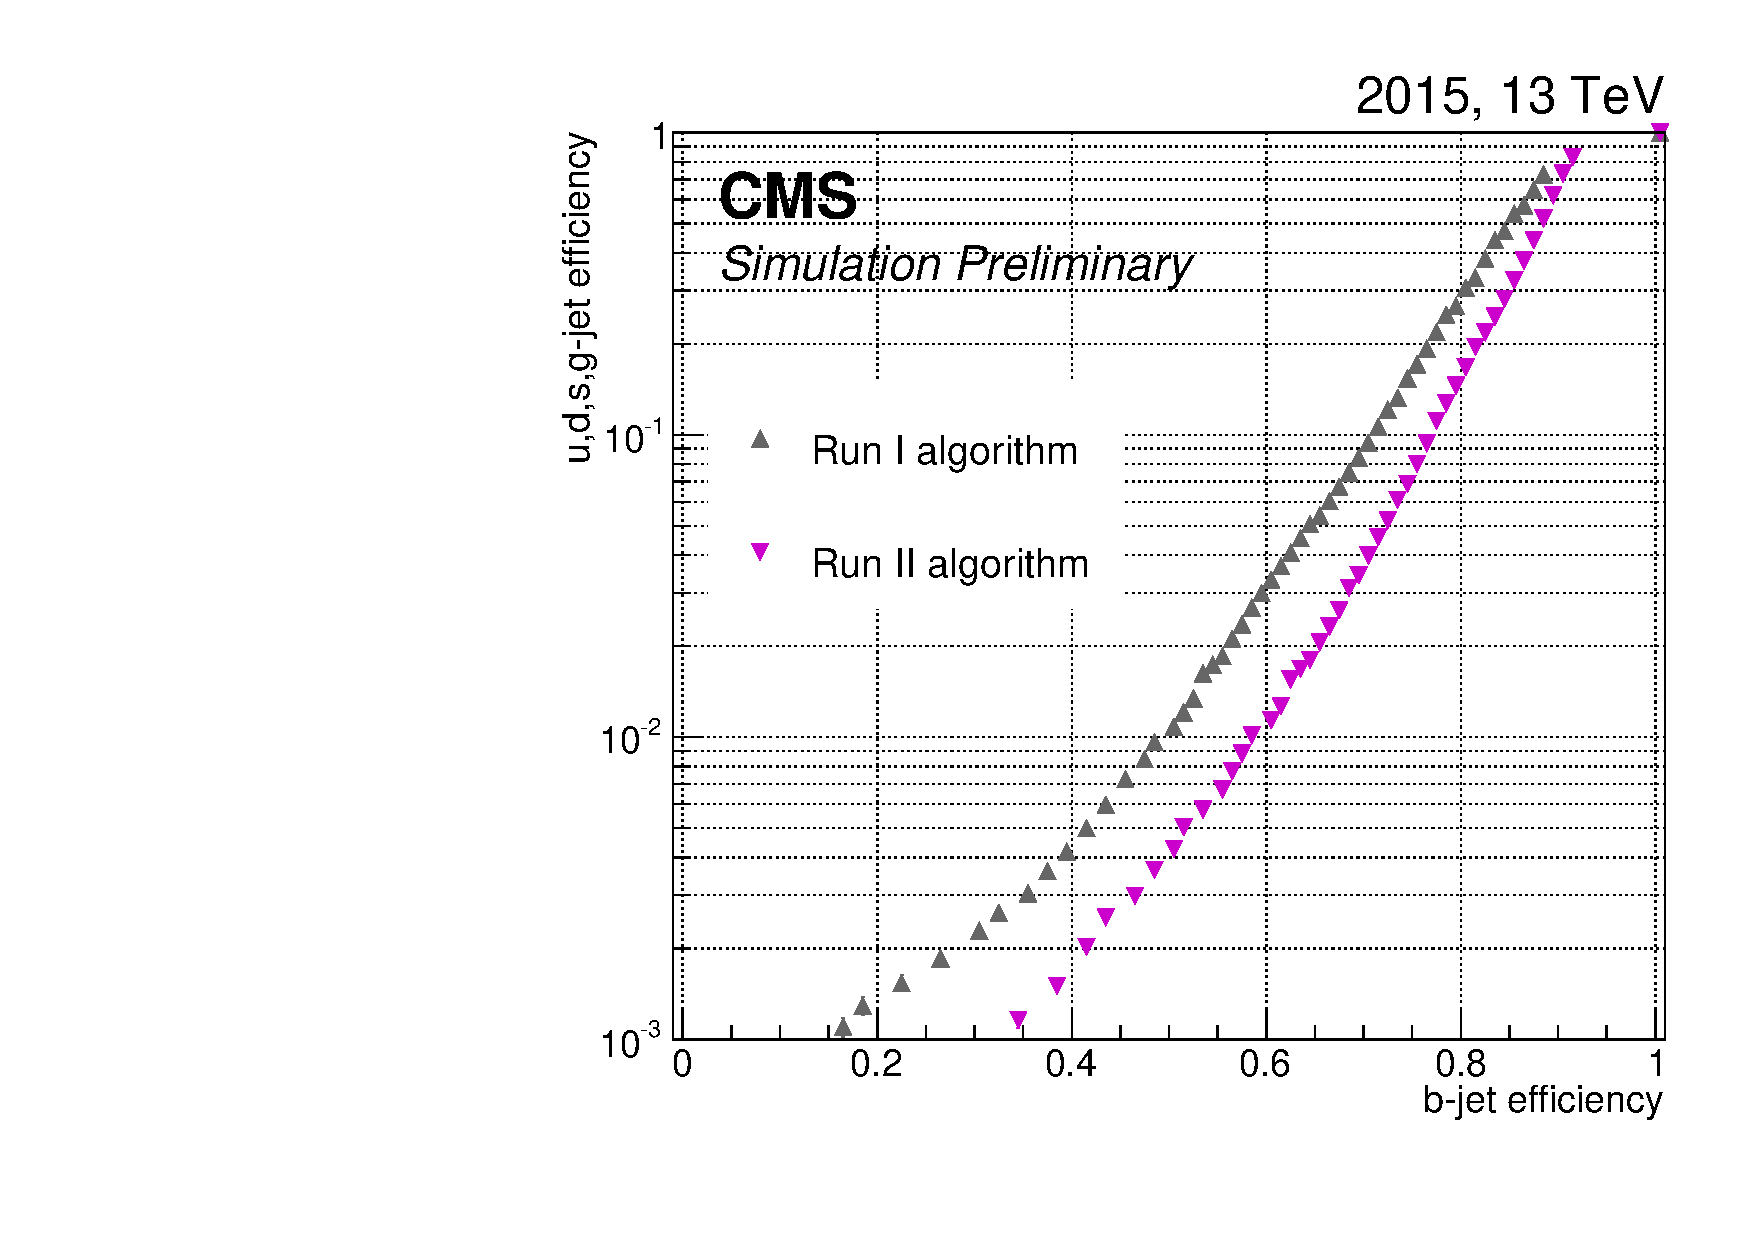
\includegraphics[width=0.45\textwidth]{figs/cms/b_udsg_RunI-II_ttbar_PU40_bx25.pdf}}
\subfigure{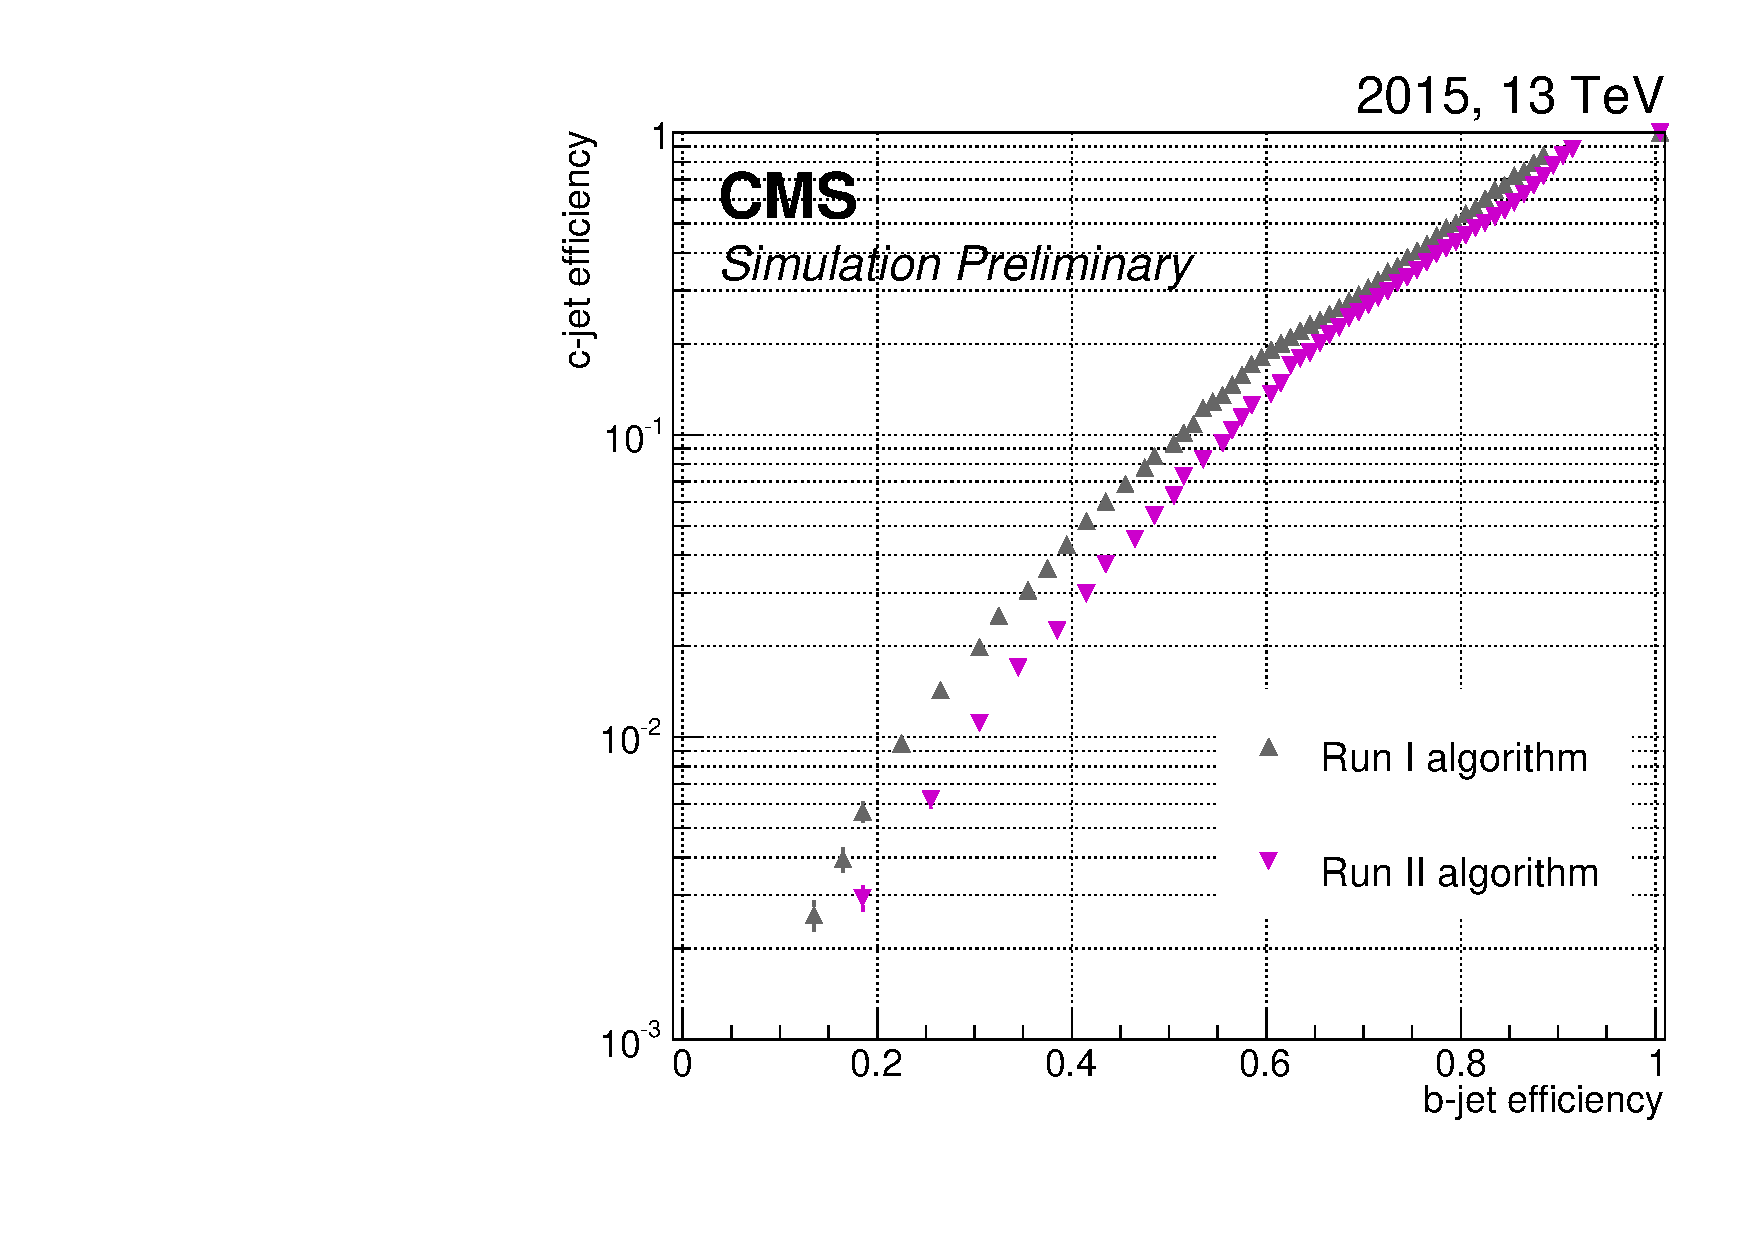
\includegraphics[width=0.45\textwidth]{figs/cms/b_c_RunI-II_ttbar_PU40_bx25.pdf}}
\caption{
Light-parton- (left) and \cPqc-jet (right) misidentification
probabilities as a function of the \cPqb-jet efficiency for the
\cPqb-jet tagging algorithms used at HLT. The gray and
magenta curves show the performance of the Run 1 and Run 2 algorithms,
respectively. 
%The Run 1 algorithm uses primary vertices made out of pixel tracks and CTF tracks as input to the CSV
%algorithm while the Run II algorithm uses iterative tracks and deterministic annealing primary vertices made out of iterative tracks
%as input to the CSVv2+IVF algorithm. 
Jets from simulated \ttbar events at $\sqrt{s} = 13$ \TeV with 40
average pileup interactions and a bunch spacing of 25 \unit{ns} are considered. 
\label{fig:mcPerformance2015}}
\end{figure}


% INFOS FROM SIMONE, DON'T REMOVE
%
% limitations of the HLT
%  time
%  paths should be independent
% 
% Even the regional tracking cannot work. 
% select events from a given L1 seed
% reconstruct calo based quantities with the same algorithms as offline
% each path defines calo-based selection, and then pf-based selection
%    so e.g. if calo MET > 80, then tracking, PF, then cut on PFMET
%
% tracking:
% reconstruct all pixel tracks as in offline (tight selections, narrow vertices)
% vertices from pixel tracks 
% take the first 3 or 4 vertices (sumpt2 + other ranking criteria)
%
% reconstruct tracks from all of these vertices and to the interesting regions. 
% 0 : start from all pixel tracks from subsample of vertices - no regions 
% 1 : define regions in which we have isolated tracks from previous iteration. 
%     combine with calo jet regions (now regional, still from same vertices)
% 2 : rinse and repeat 1 with looser seeding conditions.  


\section {Level-1 and High-Level Trigger}
\label{sec:trigger}

The role of the trigger is to reduce the rate of recorded collision to
a level which is manageable by the following data acquisition (DAQ)
and online reconstruction. At the LHC, the proton beams are organized in
bunches separated in time by 50 \unit{ns} during Run 1 (2010-2013) and 25 \unit{ns}
during Run 2 (2015-present), implying a collision rate on the order of
40 \unit{MHz}.
%in reality a bit less, because not all bunches in the machine are filled with protons
The maximum acceptable rate for data acquisition and storage is of the order of 1 \unit{kHz}, and
the trigger is designed to reduce the rate to that level, while
maintaining the largest possible acceptance of interesting physics signal
events from the collisions and efficiently rejecting the
non-interesting ones. Figure~\ref{fig:streams}

\begin{figure}\centering
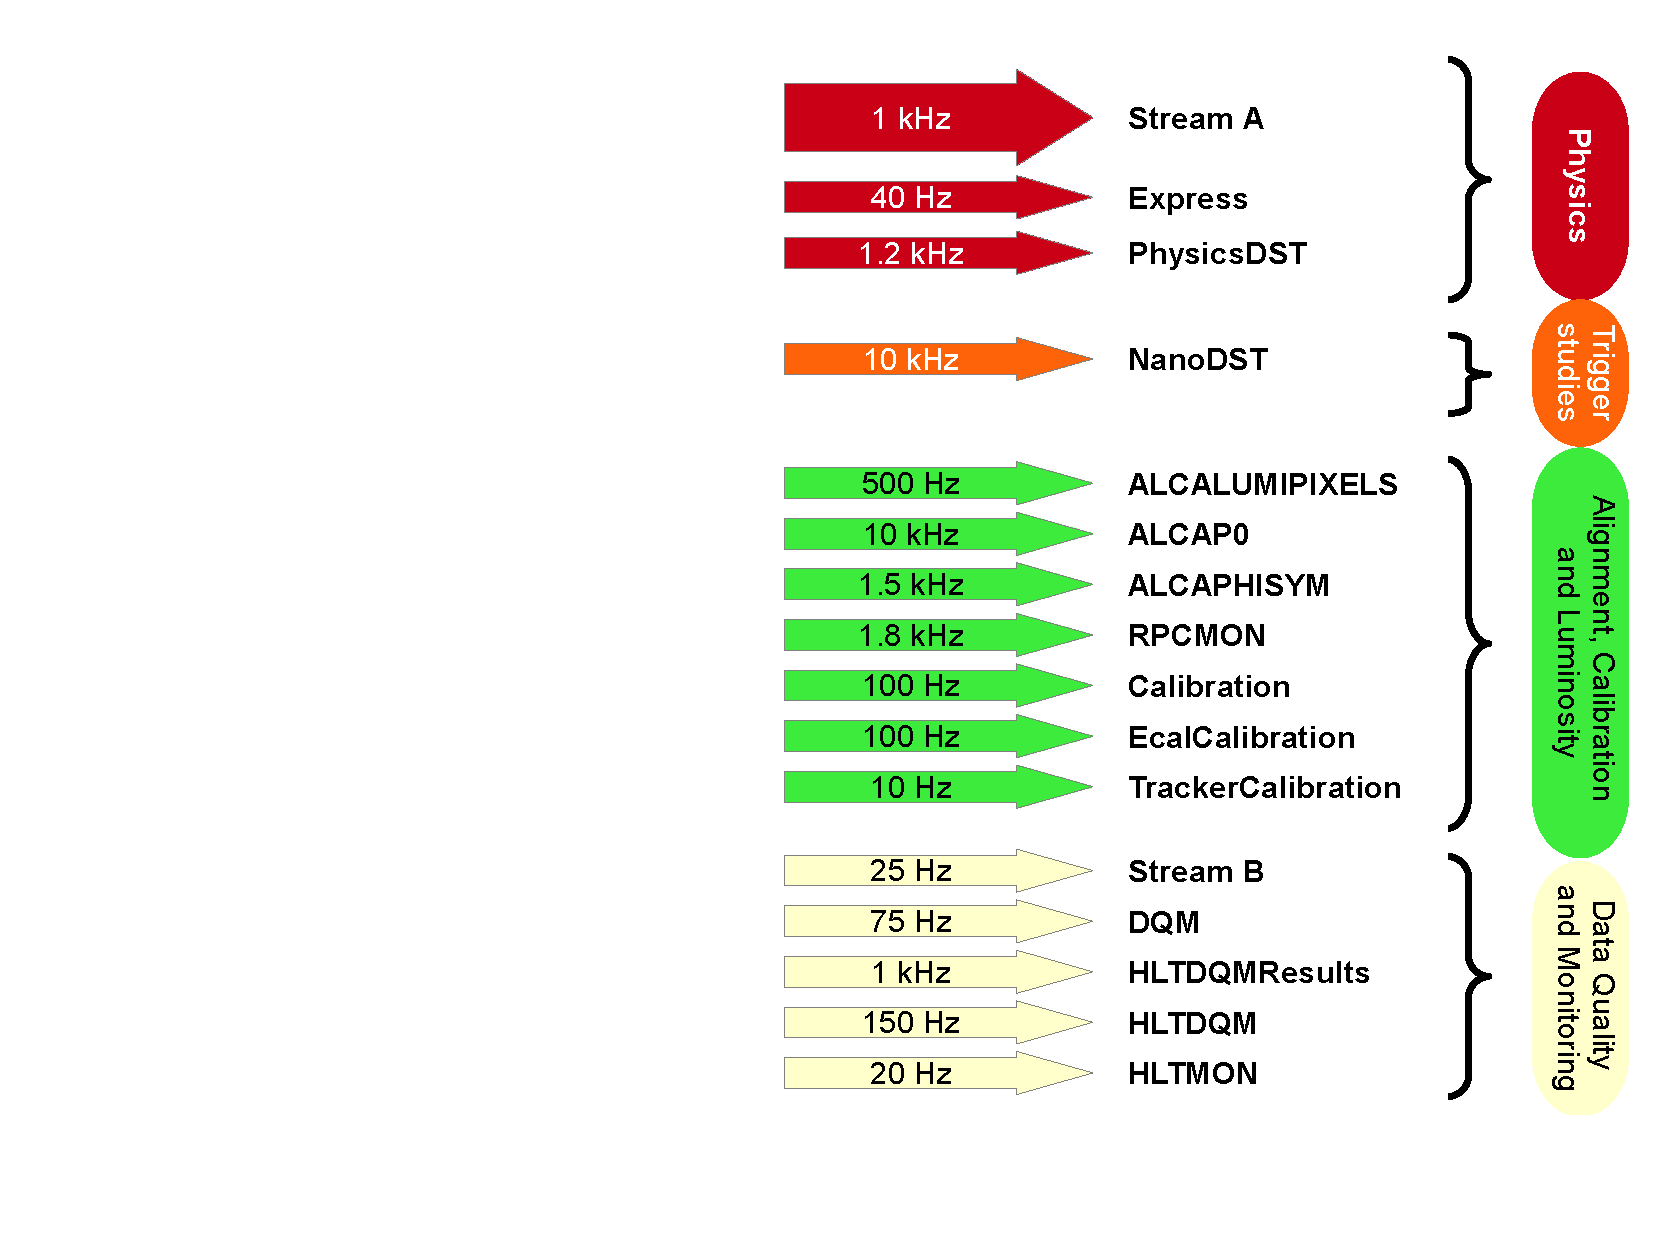
\includegraphics[width=.45\textwidth]{figs/cms/Streams2012.pdf}
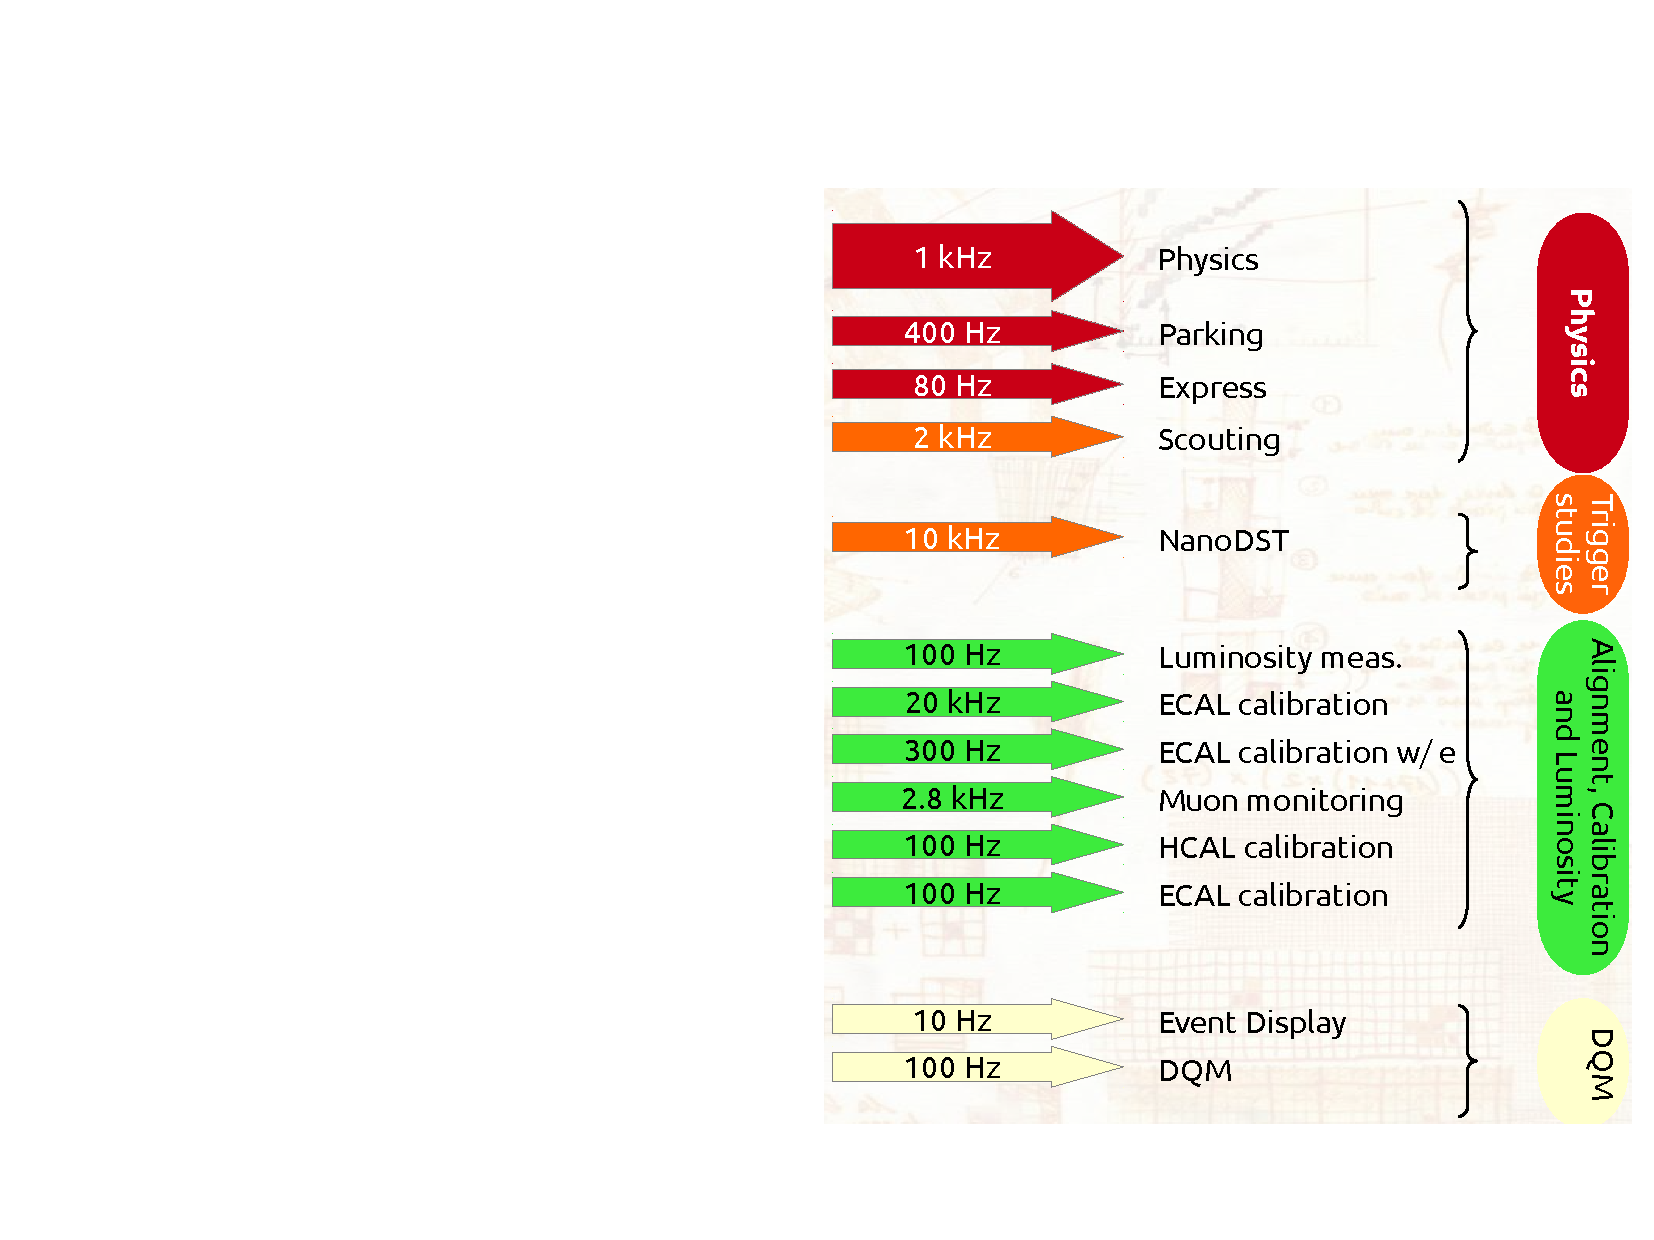
\includegraphics[width=.45\textwidth]{figs/cms/Streams2015.pdf}
\caption{Data streams during 2012 (left) and 2015 (right)
\label{fig:streams}}
\end{figure}

The design chosen for the trigger of the CMS experiment is a two-level system. The
Level 1 (L1) trigger is based on FPGA and custom ASIC technology and uses information
from the calorimeters and muon spectrometers of the experiment in order to accept or reject
an event; it reduces the event rate down to approximately 100 \unit{kHz}, acceptable by the readout
electronics. The High-Level Trigger (HLT) is implemented in software running on a farm of
commercial computers which includes approximately 16,000 CPU cores, and reduces the L1 output rate
to the sustainable level for storage and physics analysis of about 1 \unit{kHz}. The HLT software
consists of a streamlined version of the offline reconstruction
algorithms; it exploits the same software used for offline
reconstruction and analysis, optimized in order to comply with the
strict time requirements of the online selection.

The L1 trigger decision is made within a fixed time
interval of less than 4 $\mu\mathrm{s}$. The operational L1 output
rate of 100 \unit{kHz}, together with the number of CPUs in the HLT
farm, imposes a fundamental constraint on the amount of time available for the HLT to process events.
Exceeding this limit impacts the ability of CMS to collect data
efficiently. Given the CPUs available in 2015, the timing budget of the HLT is
measured to be about 300\unit{ms} when the machines are fully loaded
(or 160\unit{ms} when the machines are running a single
job)~\cite{Richardson:2015zdg}.

The HLT menu in CMS has a modular structure, which is graphically depicted in Fig~\ref{fig:modular}.
The menu is subdivided into logically independent paths, which may be
run in parallel; more than 400 different HLT paths are used for Run 2
data taking. Each path is a sequence of
reconstruction modules (producers) and filtering modules
(filters). Filters typically select events based on the properties of a given physics object (photons, electrons,
muons, jets, \ptvecmiss, \PQb-tagged jets, etc.), or, as in the case of the razor triggers
detailed in Ch.~\ref{ch:hlt13TeV}, the properties of a combination of physics objects
along with the values of topological variables $\MR$ and  $\Rtwo$. The modules
within a path are arranged in blocks of increasing complexity, so that faster
algorithms are run first and their products are filtered: if a filter fails, the rest of the path is
skipped. 

%There are other important differences between the algorithms used at HLT and
%the ones used for the offline reconstruction, intended to reduce the CPU time consumption at
%HLT. For example, some online reconstruction algorithms have a specified regionality (detector read-out and reconstruction
%are restricted to narrow regions around the L1 or higher-level
%candidates), and the tracking and PF algorithms are simplified. 

\begin{figure}\centering
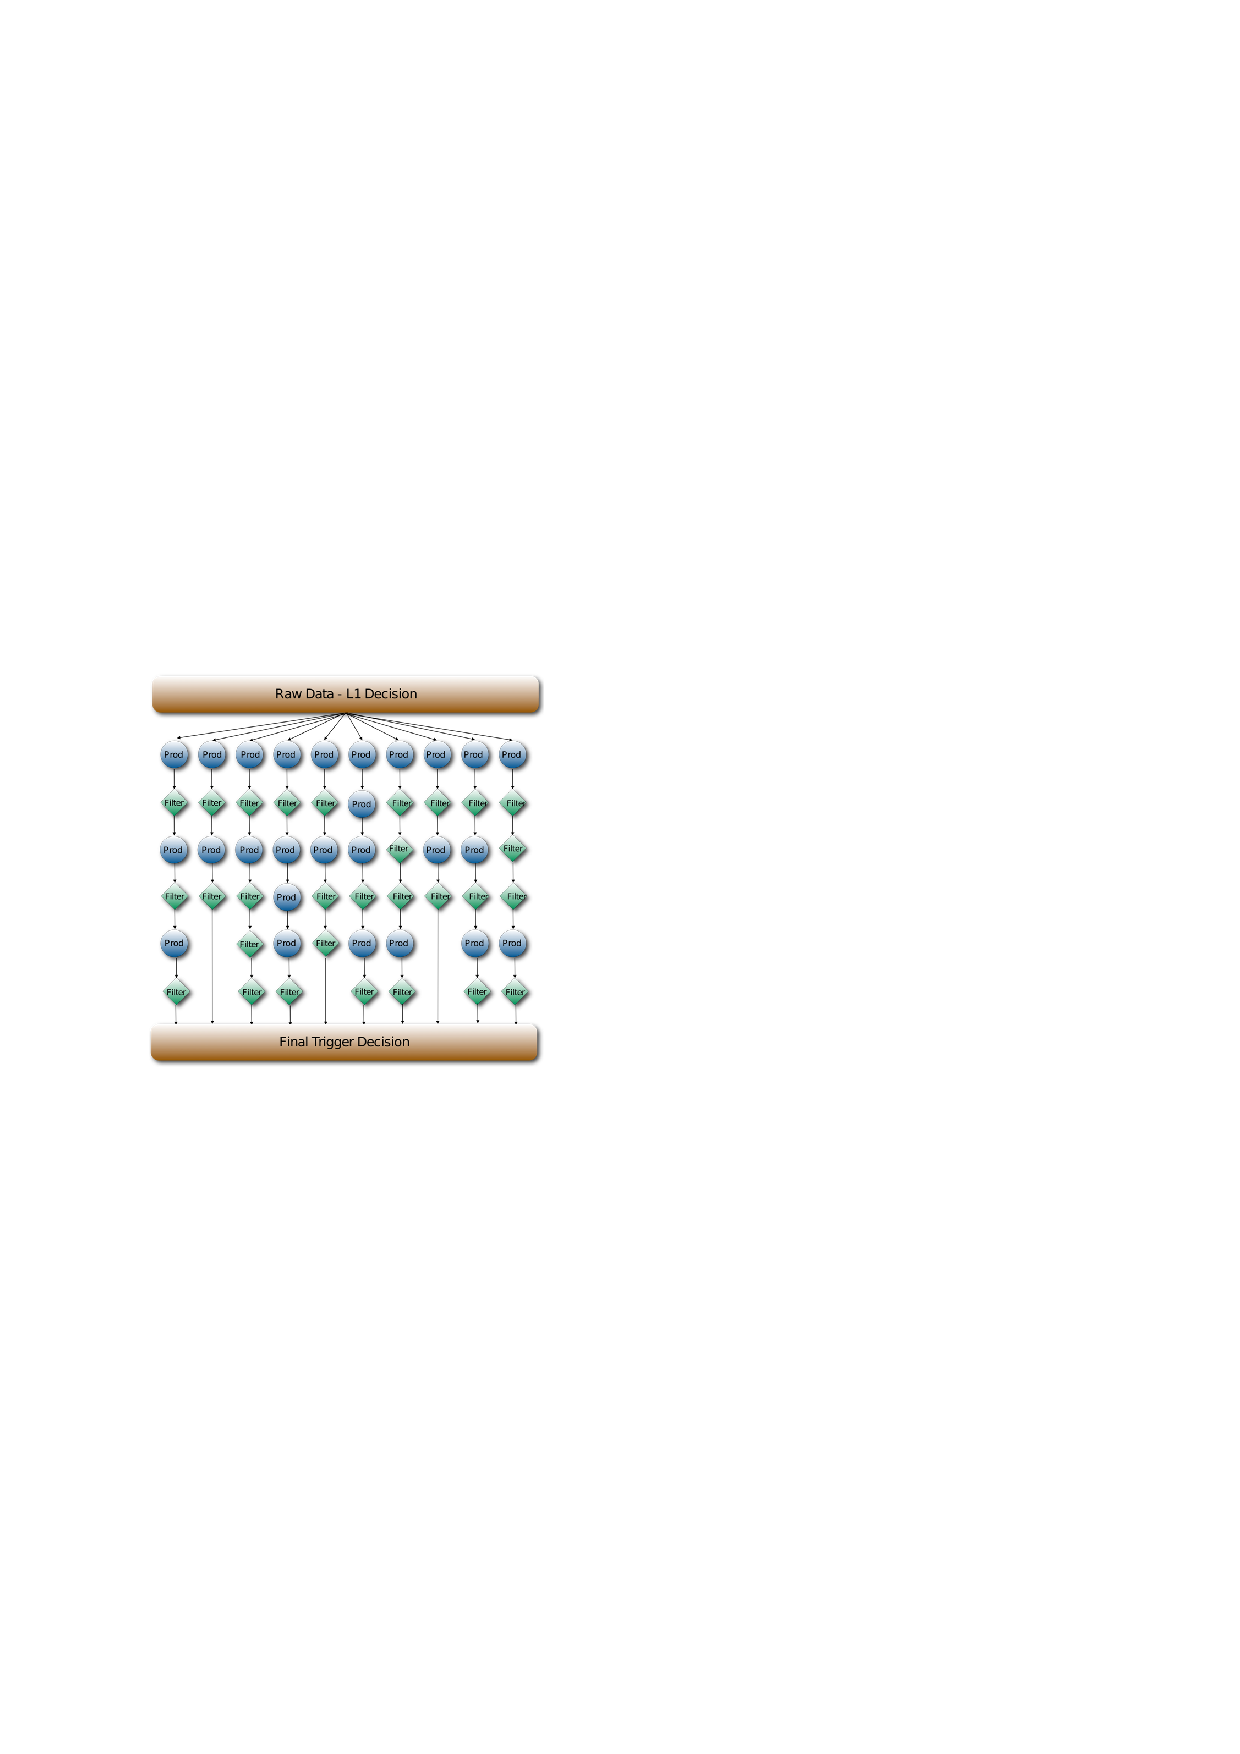
\includegraphics[width=.7\textwidth]{figs/cms/HLTschematic.pdf}
\caption{Schematic representation of the modular design of an HLT menu in CMS. The final trigger decision is the logical OR of the decisions of the single paths.
\label{fig:modular}}
\end{figure}

In order to keep the online reconstruction of physics objects at HLT as
close as possible to offline reconstruction, PF algorithms are used at
the HLT whenever possible. 
%to limit the triggering inefficiency and the false trigger rate
However, to stay within and the limited timing budget due to the
available CPU resources, the online reconstruction of a single event
for the HLT must be done more than one hundred times faster than offline on average.
Offline, most of the processing time is spent reconstructing the inner
tracks for the PF algorithm. For the HLT, the tracking is reduced to three iterations, 
dropping the time-consuming reconstruction of tracks with a low
transverse momentum or arising from nuclear interactions in the
tracker material. These modifications preserve the reconstruction efficiency for
tracks with $\pt>0.8\,\GeV$ originating from the primary vertex, even
when these tracks are produced in the decay of B mesons.
After track reconstruction, a specific instance of the particle identification and reconstruction algorithm runs online, 
with only two minor differences with respect to the offline algorithm:
the electron identification and reconstruction is not integrated in
the PF algorithm, and the reconstruction of nuclear interactions in the tracker is not performed.
The main effect of these modifications is a slightly higher jet energy
scale for jets featuring an electron or a nuclear interaction.


One of the main technical limitations of LHC data processing is the available bandwidth at which events can be
recorded on disk. Typically, this limitation forces the LHC experiments to increase the thresholds of their
triggers, in order to keep an acceptable data volume despite the
increasing collision rate.  The CMS experiment implemented special
solutions to circumvent these limitations, combining the standard
trigger approach (event filtering) with datasize reduction. By
limiting the amount of recorded information per event, one can accept
more events without allocating more bandwidth. This strategy is
adopted both for the alignment and calibration of the detector
(Sec.~\ref{sec:alca}) and for increasing acceptance to specific
physics signals (Sec.~\ref{sec:scouting}).


\section{Alignment and Calibration}
\label{sec:alca}

Fast and efficient methods for the calibration and the alignment of
the detector are a key ingredient in exploiting the physics potential of
CMS. To this end, CMS has a powerful framework for alignment and
calibration, which is based on dedicated ``skims,'' or subsets of data samples, providing a highly
compact input for the various workflows computing the
calibration and alignment constants. 
%This includes a prompt calibration concept, which allows
%for a fast turnaround of the calibration process which is instrumental
%to ensure timely preparation of results for conferences and
%publications.
%The high level of complexity and the large number of detector channels
%reflect in an elaborated structure for the management and computation
%of the detector calibration and alignment. The present contribution
%reviews the workflows developed for this purpose focusing on a few
%selected examples. 

Most of the alignment and calibration workflows are fed with dedicated
data samples, called AlCaReco datasets, optimized both in terms of event
selection and event content. Depending on the needs of the specific
workflow, these samples can be selected offline, while performing the
reconstruction, or directly online, at the HLT level. 
%The great
%flexibility of the HLT, which runs offline-quality software on a farm of commercial processors, is a key asset for this
%online selection since it guarantees an adequate rate of events that
%would not be selected by the standard trigger paths meant for physics
%analysis.

An example of an online calibration stream is the one selecting events
containing $\pi^0$ and $\eta$ candidates detected in the ECAL and used
for the intercalibration of the PbWO$_4$ scintillating
crystals~\cite{Chatrchyan:2013dga}. The calibration performance
depends on the number of selected $\pi^0$ candidates per crystal and
on the signal-to-background ratio. The candidate diphoton decays are
selected at the HLT level from events passing single-$e/\Pgg$ and
single-jet L1 triggers. After selection, only information about a
limited region of ECAL (energy deposits in $20$ to $40$ individual
crystals) near the $\pi^0$ candidates is stored for the actual
calibration. This allows to sustain a high rate of calibration events
($1$ to $10$ kHz) whilst saving bandwidth and CPU time.


Detector conditions that change on a short time scale require a special
calibration workflow designed to allow updates with very short
latency. To meet this need, the organization of data streams is as follows:
\begin{itemize}
\item express processing: reconstruction of a limited selection of
  data in order to give quick feedback about the detector status and
  physics performance and to provide data for calibration
  workflows. The results of the express reconstruction for a given run
  are usually available one or two hours after the raw data are
  collected;
\item bulk processing: reconstruction of the main data stream for
  physics analysis. This step, called prompt reconstruction, is
  delayed by 48 hours to allow for the computation and usage of 
  new calibration constants relating to fast-changing conditions. The output is divided in
  several Primary Datasets (PD) on the basis of the HLT paths that select the events;
\item calibration streams: streams of events selected at the HLT level
  and processed at Tier-0 for calibration purposes.
\end{itemize}

During Run 1 normal operation, about $300-400$\unit{Hz} of data 
were processed in the bulk processing, while about $30-40$\unit{Hz} was allocated for express
processing in order to guarantee a fast reconstruction. A selection of
data from the express and calibration streams is used
to compute the updated conditions for a given run while the bulk of
the data is buffered on disk. The calibration workflows run on a
dedicated farm at CERN called the CMS Analysis Facility (CAF). In this
way the prompt reconstruction can profit from the updated constants,
reducing the need for offline reprocessing of the data. This workflow
is called the \emph{prompt calibration loop} and is illustrated schematically
in Fig.~\ref{fig:AlCa}. The conditions currently updated through this kind of
workflow are:
\begin{itemize}
\item measurement of the beam-line parameters;
\item monitoring and masking of problematic channels of the silicon strip tracker to respond to
HV trips or noise;
\item transparency corrections based on the laser monitoring system for the PbWO$_4$ crystals of the ECAL
  calorimeter.
\end{itemize}
The delayed prompt reconstruction is also exploited to
monitor possible movements of large structures of the silicon tracker,
mainly due to thermal stress, and problematic channels in the
electromagnetic and hadronic calorimeters allowing for quick reaction
time in case of ``hot'' regions identified in the express
reconstruction.

\begin{figure}\centering
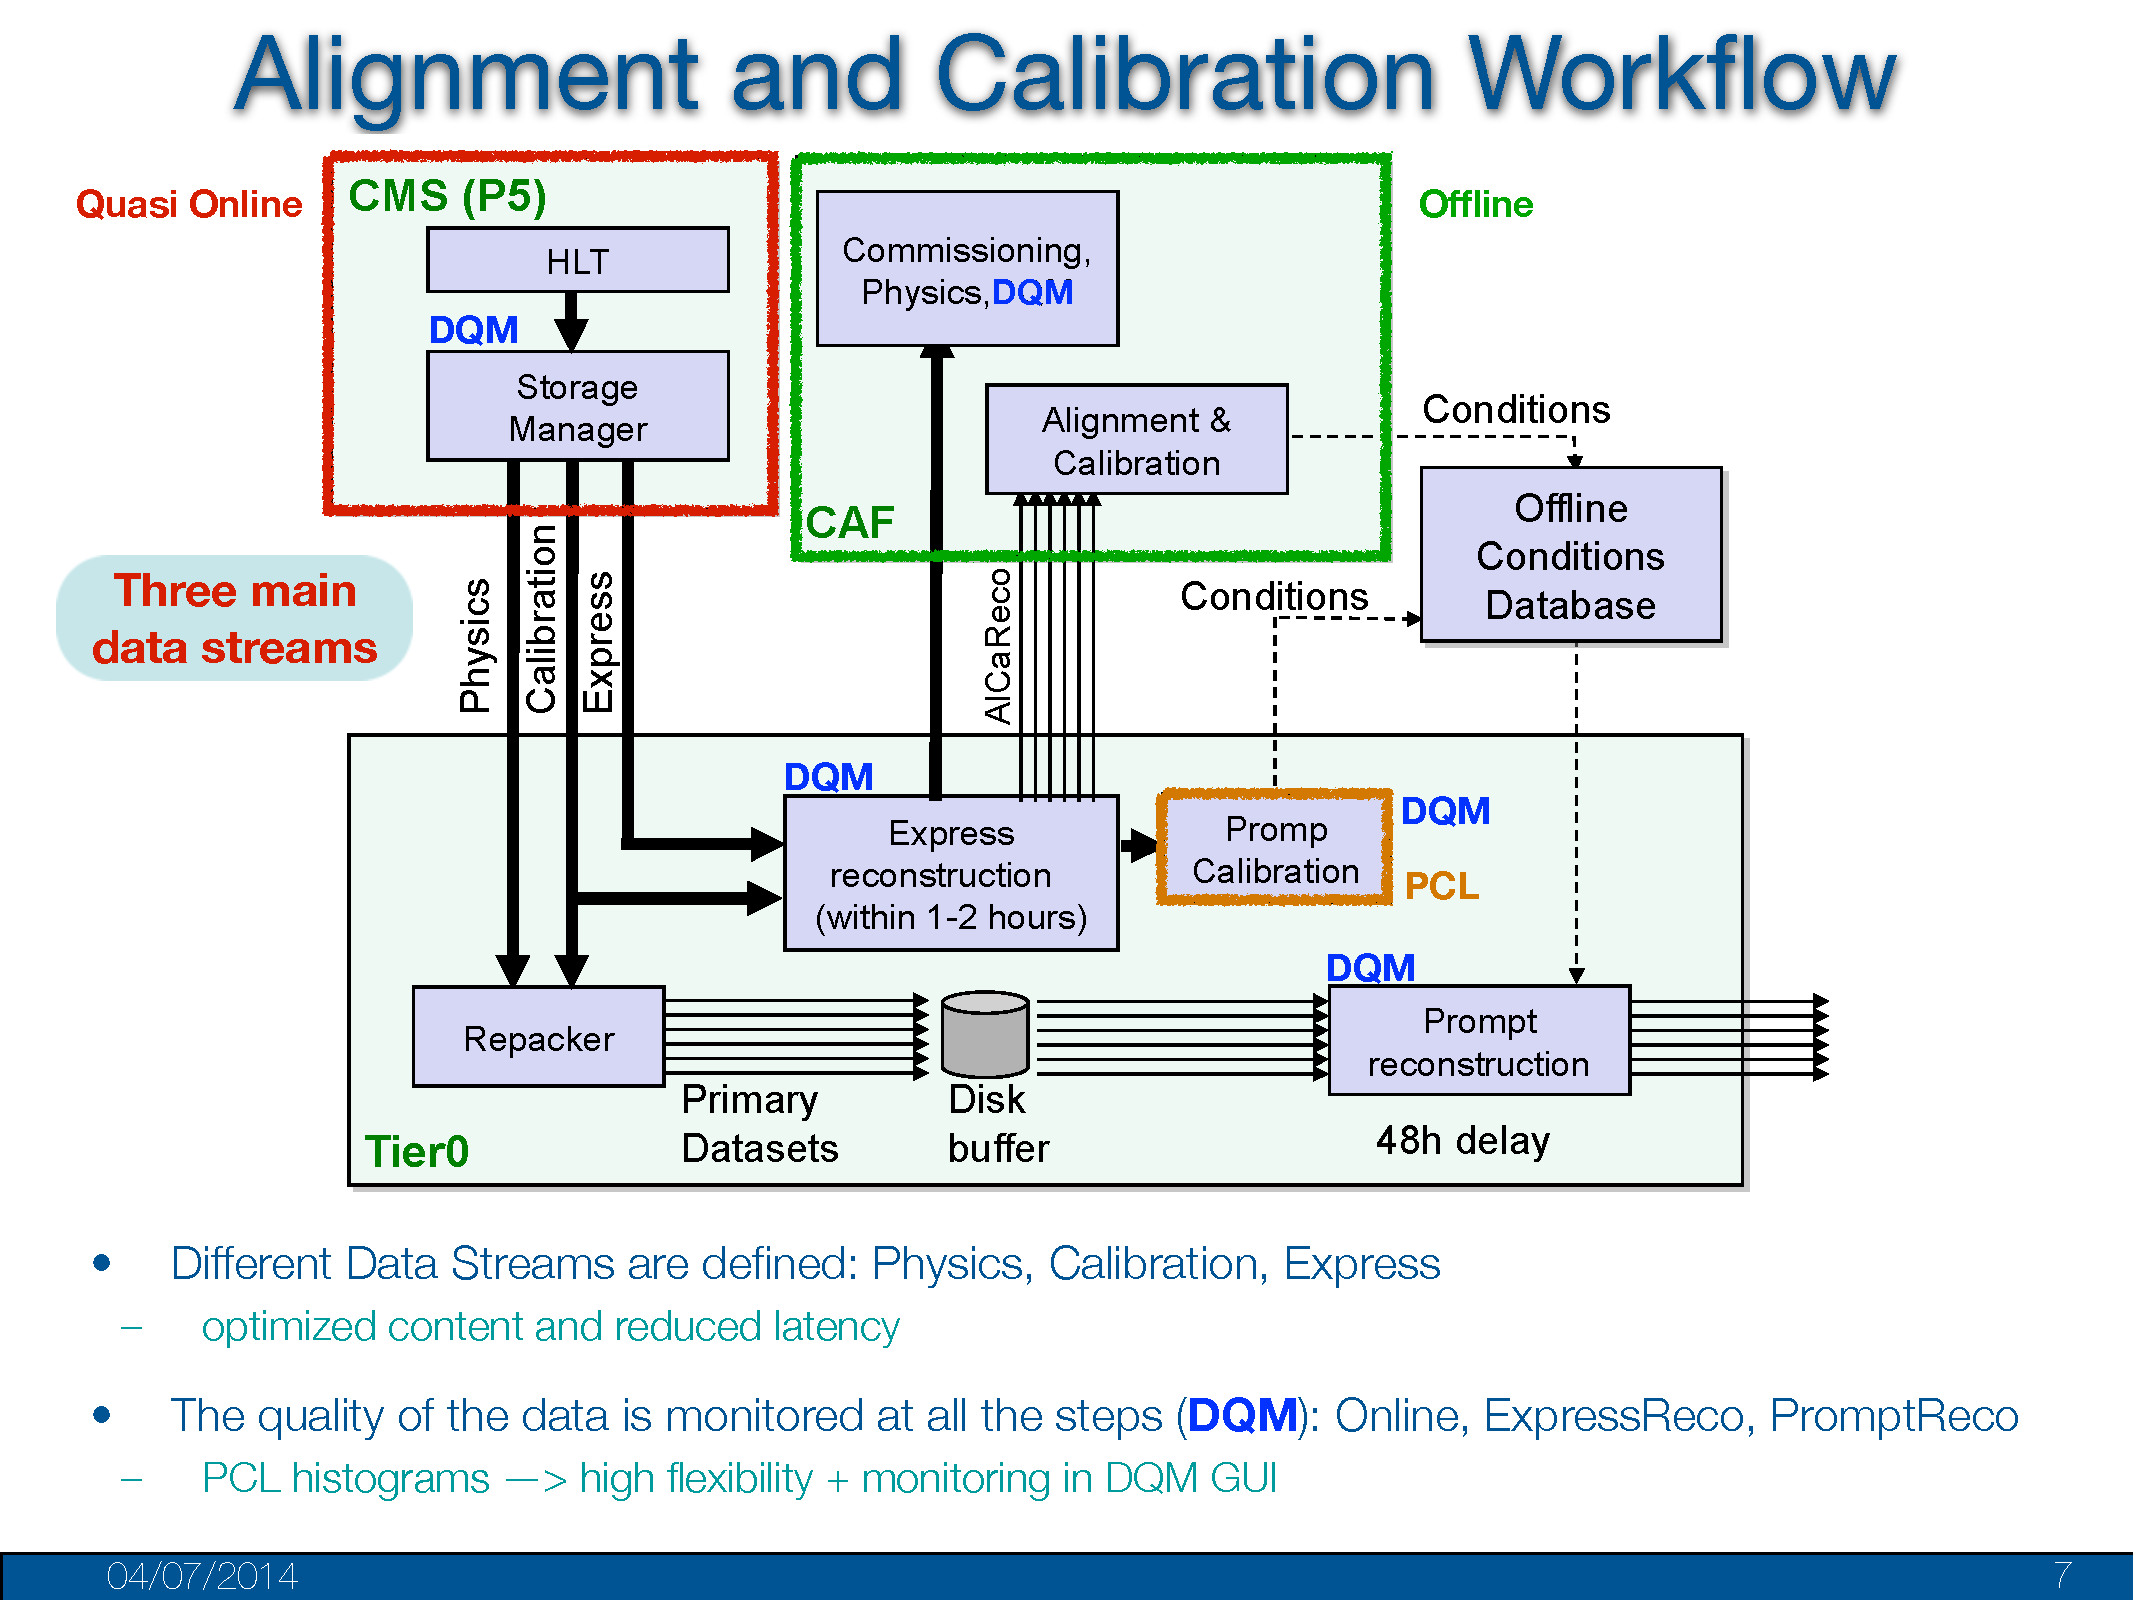
\includegraphics[width=.9\textwidth,clip=true,viewport=0 180 900 700]{figs/cms/AlCa.pdf}
\caption{Alignment and calibration data-processing flow.\label{fig:AlCa}}
\end{figure}

In order to reach the ultimate accuracy, more sophisticated
alignment and calibration workflows are run offline. No time
constraints are present in this case and the full treatment of the
detector’s alignment and calibration inter-dependencies can be
studied and taken into account. The full data sample is exploited to
provide the final set of conditions which are then used in the
reprocessing of the data. In normal conditions the full dataset is
reprocessed once per year. Some important offline workflows are as follows:
\begin{itemize}
\item energy calibration of the ECAL response (single channel and overall energy scale calibration);
\item measurement and correction of the tracker orientation with respect to the magnetic field;
\item tracker module alignment.
\end{itemize}

A third class of calibration workflows, the quasi-online calibration,
is meant to update conditions at HLT for data taking. %The measurement
%of the beam-line parameters falls in this category as well. 
For some very stable corrections that do not need to be validated, such as the measurement of beam-line
parmaters, an application running in the Data Quality Monitoring (DQM)
framework~\cite{DeGuio:2014taa} automatically derives and stores conditions in a database which is
then accessed at the HLT during the online event
reconstruction. This feedback from the DQM to the HLT happens with a
time granularity of 2 minutes (5 luminosity sections).
For other corrections that do need to be validated, such as the ECAL transparency
corrections, a validation workflow is run, involving ECAL experts who
derive, carefully check, and upload the corrections to the database on
a weekly basis during data taking.


\subsection{ECAL Laser Monitoring}

The crystals have to withstand the damage to the crystal
lattice caused by radiation expected throughout the duration of LHC operation. The
expected integrated ionizing dose in the ECAL is up to $4$ \unit{kGy} in the
barrel and $200$ \unit{kGy} at $\abs{\eta} = 3$ after $10$ years of LHC operation
corresponding to an integrated luminosity of $500$ \fbinv~\cite{CMSECALTDR}. The
expected hadron fluence varies between about $10^{13}$ cm$^{-2}$ in the barrel
and $10^{14}$ cm$^{-2}$ at $\abs{\eta} = 3$. The main observable effect of the radiation
is a wavelength-dependent loss of crystal transparency due to the
formation of color centers, but without changes to the scintillation
mechanism~\cite{Adzic:2009aa}. In order to measure and correct for
response change during LHC operation, the ECAL is equipped with a
light monitoring (LM) system~\cite{Anfreville:2007zz,Zhang:2005ip}. 

The evolution of the ECAL response to the laser light (440 \unit{nm} in 2011 and 447 \unit{nm} from 2012 onwards) from 2011
through 2016 is shown in Fig.~\ref{fig:ECALLaserHistory}, as a function of time~\cite{CMS-DP-2016-031}. 
%An average value is shown for each of six pseudorapidity ranges. The data are normalized to the
%measurements at the start of 2011. The corresponding instantaneous
%luminosity is also shown. 
The response drops during periods of LHC operation, and recovers
during shutdown periods (or periods of low-luminosity data-taking). These
observations correspond to changes in crystal
transparency~\cite{Adzic:2009aa} and are used to correct the physics
data. The response change observed in the ECAL channels is up to 6\% in the
barrel and it reaches up to 30\% at $\abs{\eta} \sim 2.5$, the limit
of the tracker acceptance. The response change is up to 70\% in the
region closest to the beam pipe. 

%A second effect of the
%radiation is that the VPT response decreases with accumulated
%photocathode charge to a plateau [17]. Radiation does not affect the
%gain of the APDs but in large doses induces dark currents which cause
%small reductions in the bias voltage at the APDs if not compensated
%for. 

\begin{figure}\centering
%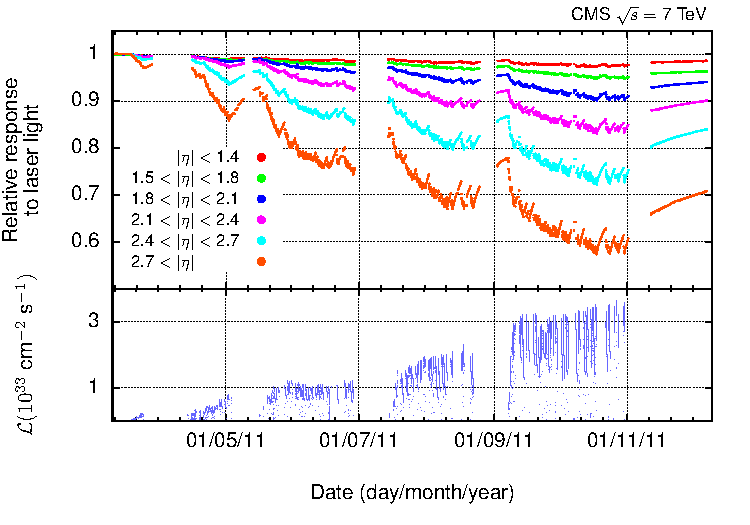
\includegraphics[width=.9\textwidth]{figs/cms/histories_2011_v2.pdf}
\includegraphics[width=.9\textwidth]{figs/cms/histories_2016.pdf}
\caption{Relative response to laser light from 2011 to 2016, normalized to
  data at the start of 2011. An average is shown for each
  pseudorapidity range. The bottom plot shows the corresponding
  instantaneous luminosity. After each LHC technical stop, a
  recovery of crystal transparency is observed.\label{fig:ECALLaserHistory}}
\end{figure}

The ECAL light monitoring system is used to determine corrections,
denoted $S(t)$, to response changes in the ECAL. The
laser light is injected through optical fibers in each crystal. The spectral
composition and the path for the collection of laser light at the
photodetector are different from those for scintillation light. A
conversion factor is required to relate the changes in the ECAL
response to laser light to the changes in the scintillation
signal. The relationship is described by a power law~\cite{CMSECALTDR}:
\begin{equation}
\frac{S(t)}{S_0} = \left(\frac{R(t)}{R_0}\right)^{\alpha}~,
\end{equation}
where $S(t)$ is the channel response to scintillation light at a particular time $t$, $S_0$ is the initial
response, and $R(t)$ and $R_0$ are the corresponding response to laser
light. The exponent $\alpha$ is independent of the loss for small
transparency losses and was measured in test beams to be $1.52$ and
$1.0$ for crystals from the two different
producers~\cite{VanLysebetten:787485,Adzic:2006za,Ghezzi:934066}.

Different forms of these laser corrections, differing in time and
spatial granularity, are utilized at different
times in the data processing: online at the HLT, during the prompt
reconstruction, and during offline reprocessing of the data. At HLT,
the laser corrections are updated once-per-week and are applied to 11
different $\eta$ rings in each endcap and 17 different $\eta$ rings in
the barrel (the corrections are averaged over each ring). For the prompt reconstruction and the offline
reprocessing, the laser corrections are updated every 40 minutes
and are applied crystal-by-crystal.

The validation of the HLT laser corrections uses a custom workflow which
re-runs the HLT reconstruction on recently collected data with two versions of
laser corrections: the version currently online (and now out-of-date)
and the version to be validated (and up-to-date). An example of a
successfully validated HLT laser correction for a particular week of
data-taking in 2015 is shown in Fig.~\ref{fig:ECALHLT}. Unlike the
outdated laser corrections (shown in blue), the updated
laser corrections (shown in black) correct the energy response and
improve the energy resolution for both the endcaps and the barrel.

\begin{figure}\centering
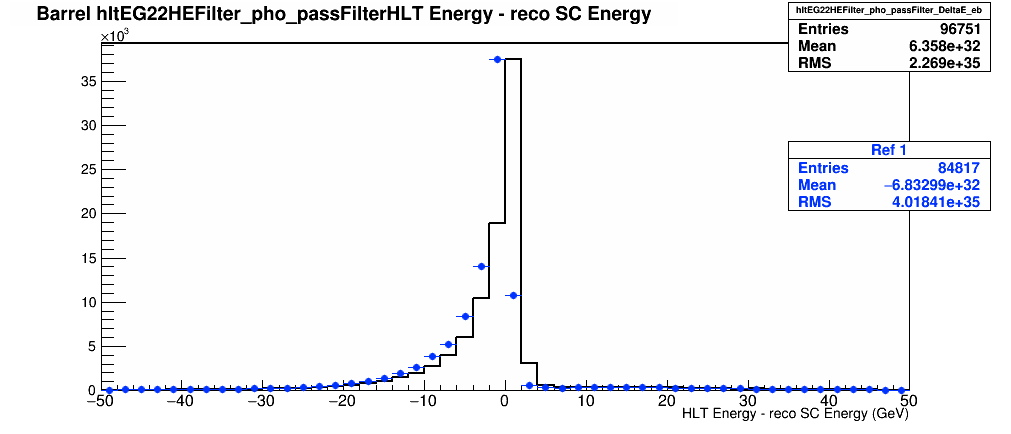
\includegraphics[width=.9\textwidth]{figs/cms/Week42_transpCorr_EB_overlay_IntermediateBlack_oldBlue.png}\\
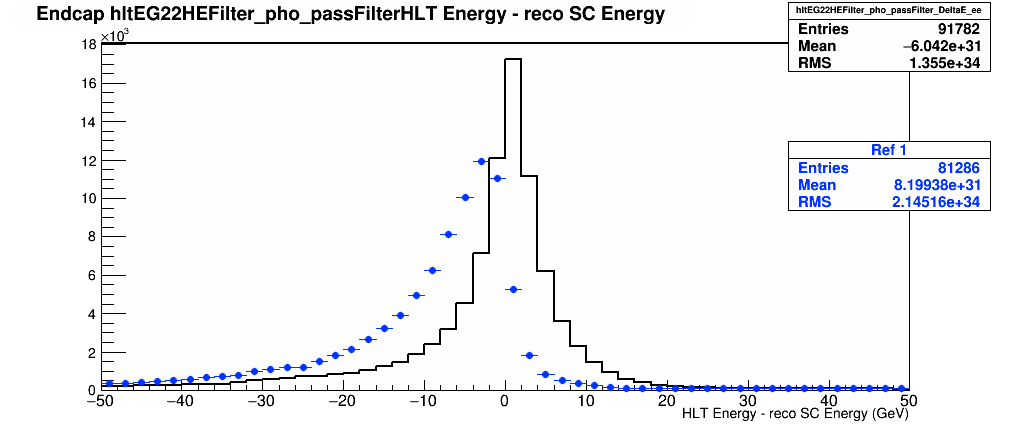
\includegraphics[width=.9\textwidth]{figs/cms/Week41_transpCorr_EE_overlay_newBlack_oldBlue.png}
\caption{The top (bottom) plot shows the difference between the supercluster energy
  reconstructed at HLT and a reference energy for the ECAL barrel (endcaps) for a particular
  week of data-taking in 2015. The blue data points show the
  difference using the week-old laser corrections, while the solid black histogram shows the reconstructed energy with the
  updated laser correction undergoing validation.\label{fig:ECALHLT}}
\end{figure}
%https://twiki.cern.ch/twiki/bin/viewauth/CMS/EGammaHLT2015LaserCorrValWeeklyReport

The $\Pgh$ meson data are used to validate the laser corrections for prompt reconstruction. The events are
selected online by a dedicated calibration trigger and recorded with
reduced event content. A fit is carried out on the invariant mass distribution of the photon
pairs in the mass range of the $\Pgh$ meson. The fit comprises a
polynomial function to describe the background and a Gaussian
distribution to describe the resonance peak. Fig.~\ref{fig:etaEB}
shows an example of the $\Pgh$-meson peak with the fit superimposed,
and the relative value of the fitted $\Pgh$ mass versus time in EB for
a period of 60 hours. The plot shows the data before (red points) and
after (green points) the laser corrections applied. A number of
measurements are possible for each LHC fill, owing to the high
rate for recording $\Pgh$ events. This permits short-term changes in
the ECAL response to be verified before the prompt reconstruction
takes place.

\begin{figure}[bht]
\begin{center}
 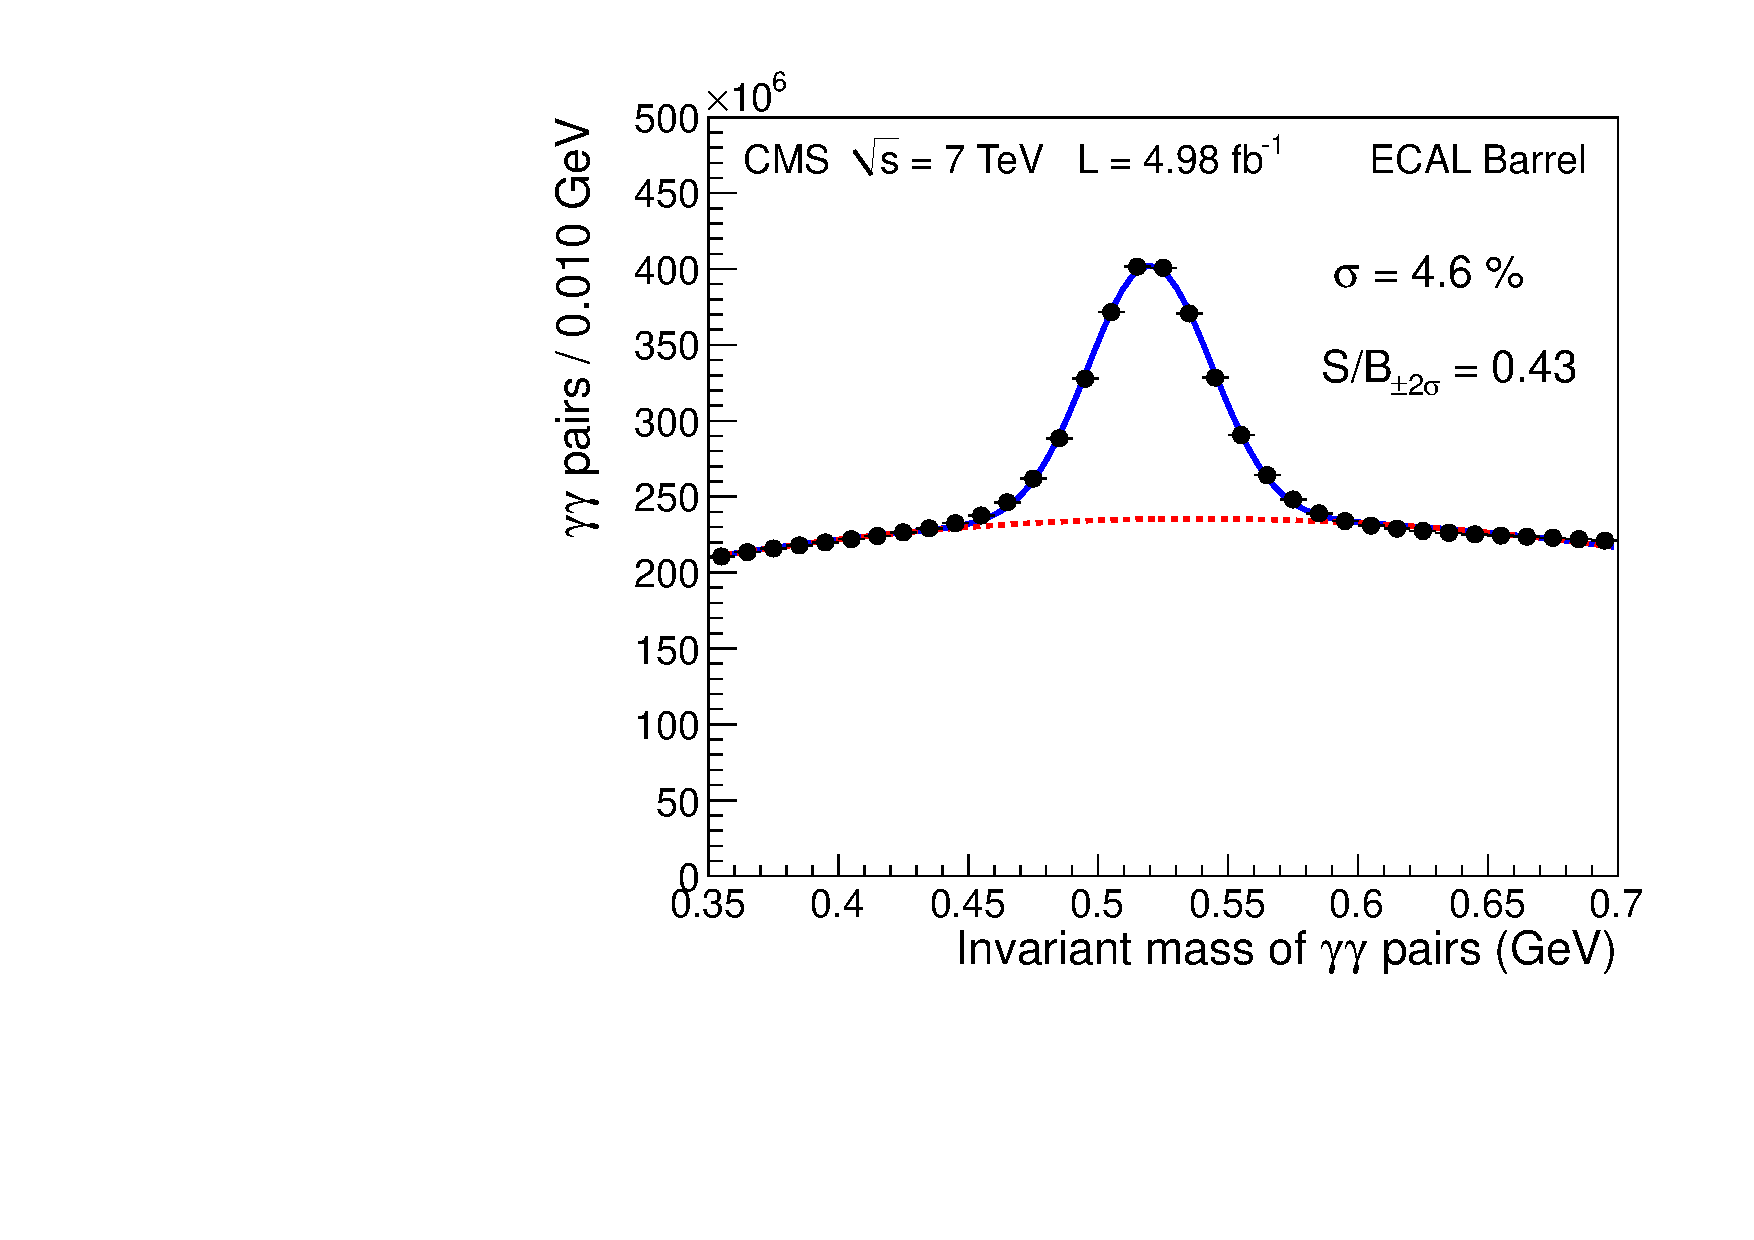
\includegraphics[width=0.40\linewidth,height=5.6cm]{figs/cms/eta_peak.pdf}
 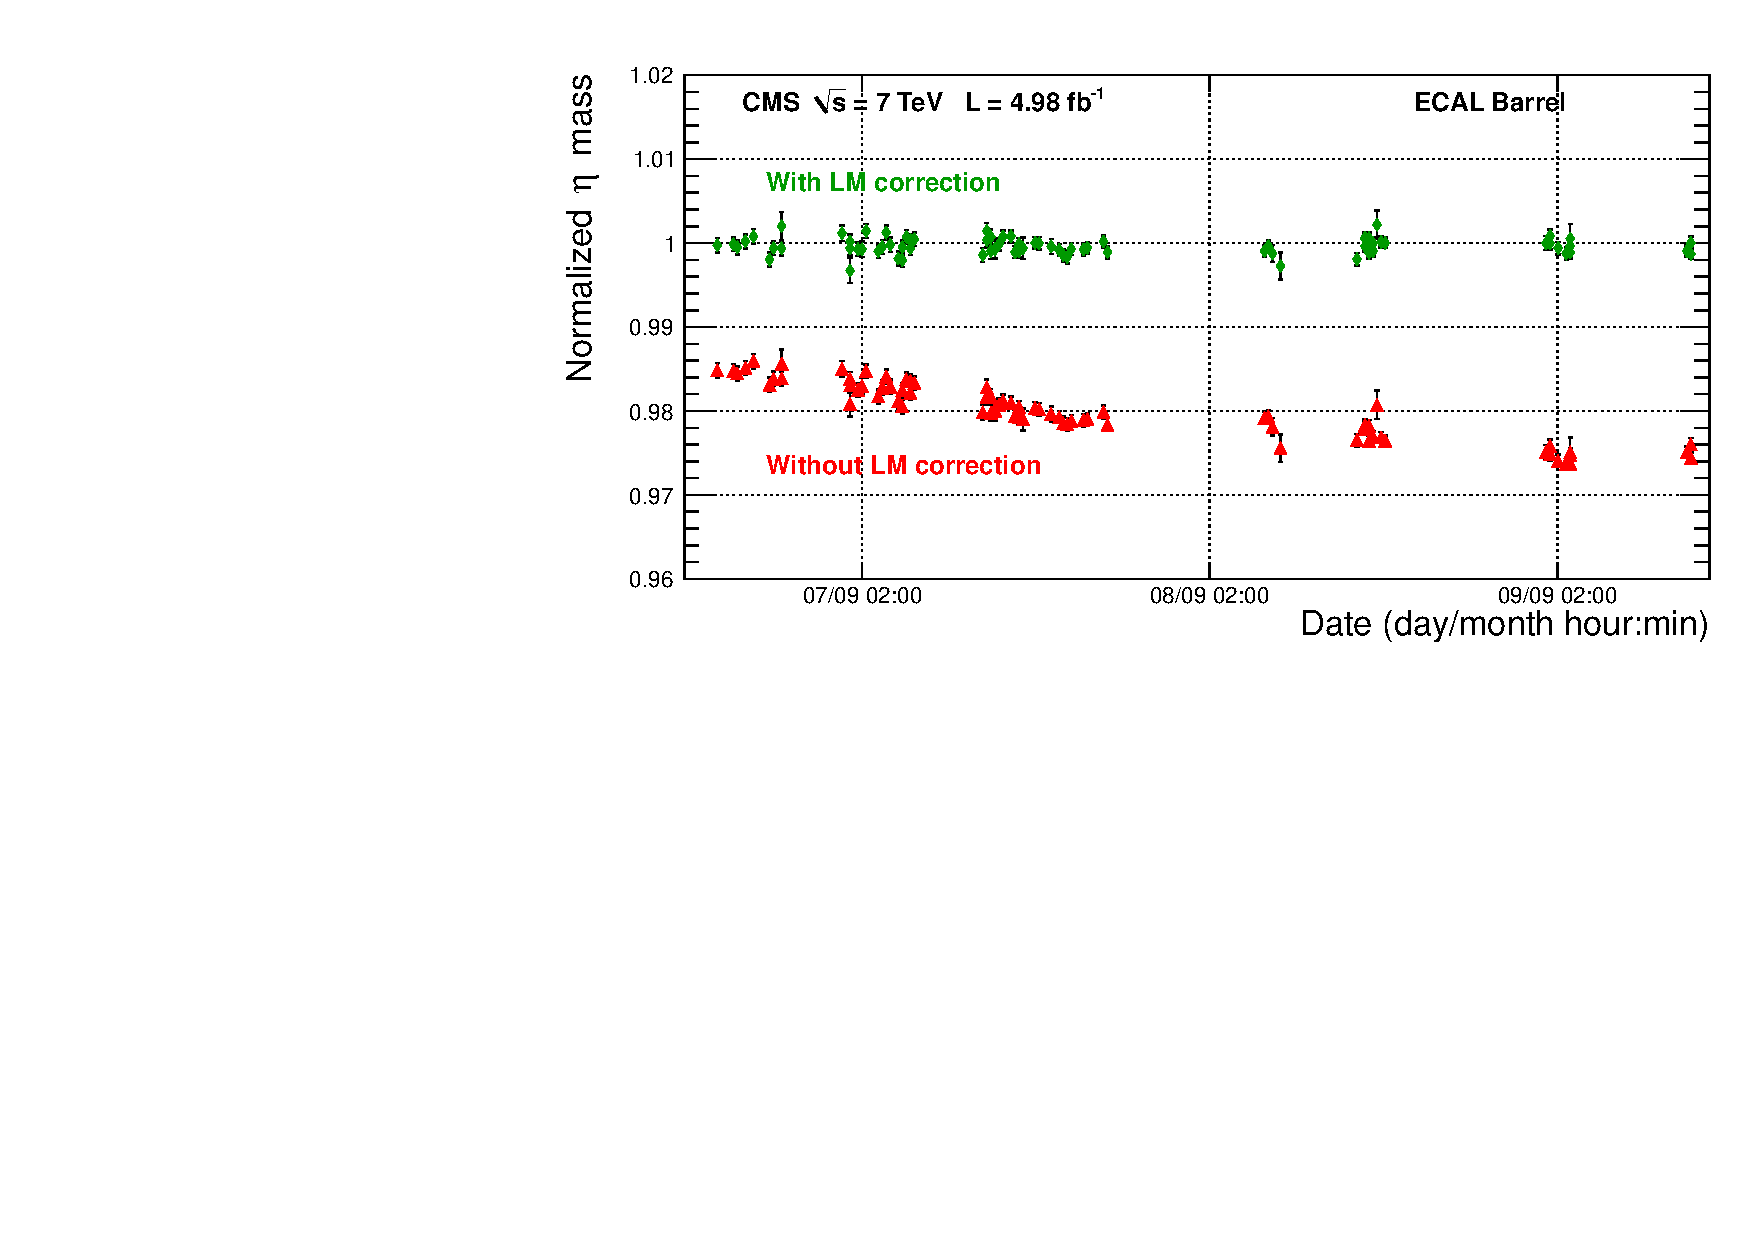
\includegraphics[width=0.59\linewidth,height=5.6cm]{figs/cms/eta_zoom.pdf}
\end{center}
\caption{\label{fig:etaEB}
Left: An example of the $\Pgh$-meson peak reconstructed from the invariant
mass of photon pairs in the barrel, with the result of the fit with a Gaussian
distribution (continuous line) and a polynomial function (dotted line);
Right: Stability of the $\Pgh\to\Pgg\Pgg$ mass measurement in the barrel as a
function of time, over a period of 60 hours, for data recorded in
September 2011. The plot shows the data with (green points) and
without (red points) laser corrections applied.}
\end{figure}

Finally, isolated electrons from $\PW$-boson decays are used to provide an energy
scale to validate the laser corrections over periods of days to
weeks. The event selection is described
in~\cite{EGM-10-004,Khachatryan:2010xn}.
The ratio of the electron energy, $E$, measured in the ECAL, to the
electron momentum, $p$, measured in the tracker, is computed in each
event, and a reference $E/p$ distribution is obtained from the entire
data set after applying laser corrections. The width of the $E/p$
reference distribution is dominated by the energy and momentum
resolution and is not biased by residual imperfections in the laser
corrections. This reference distribution is then scaled to fit
$E/p$ distributions obtained by dividing the same data in groups of
12000 consecutive events. The scale factors provide a measure of the
relative response and are shown in Fig.~\ref{fig:wenuEB} for 2011, as
a function of time. The data are shown before (red points) and after
(green points) laser corrections to the ECAL channel response are
applied. The magnitude of the average correction for each point is
indicated by the continuous blue line. A stable response to
electromagnetic showers is achieved throughout 2011 with an RMS of
0.12\% in the barrel and 0.35\% in the endcaps. This method does not require a
knowledge of the absolute calibration of both the energy and the
momentum.

\begin{figure}
\begin{center}
\begin{tabular}{cc}
 \hspace{-0.5cm}
 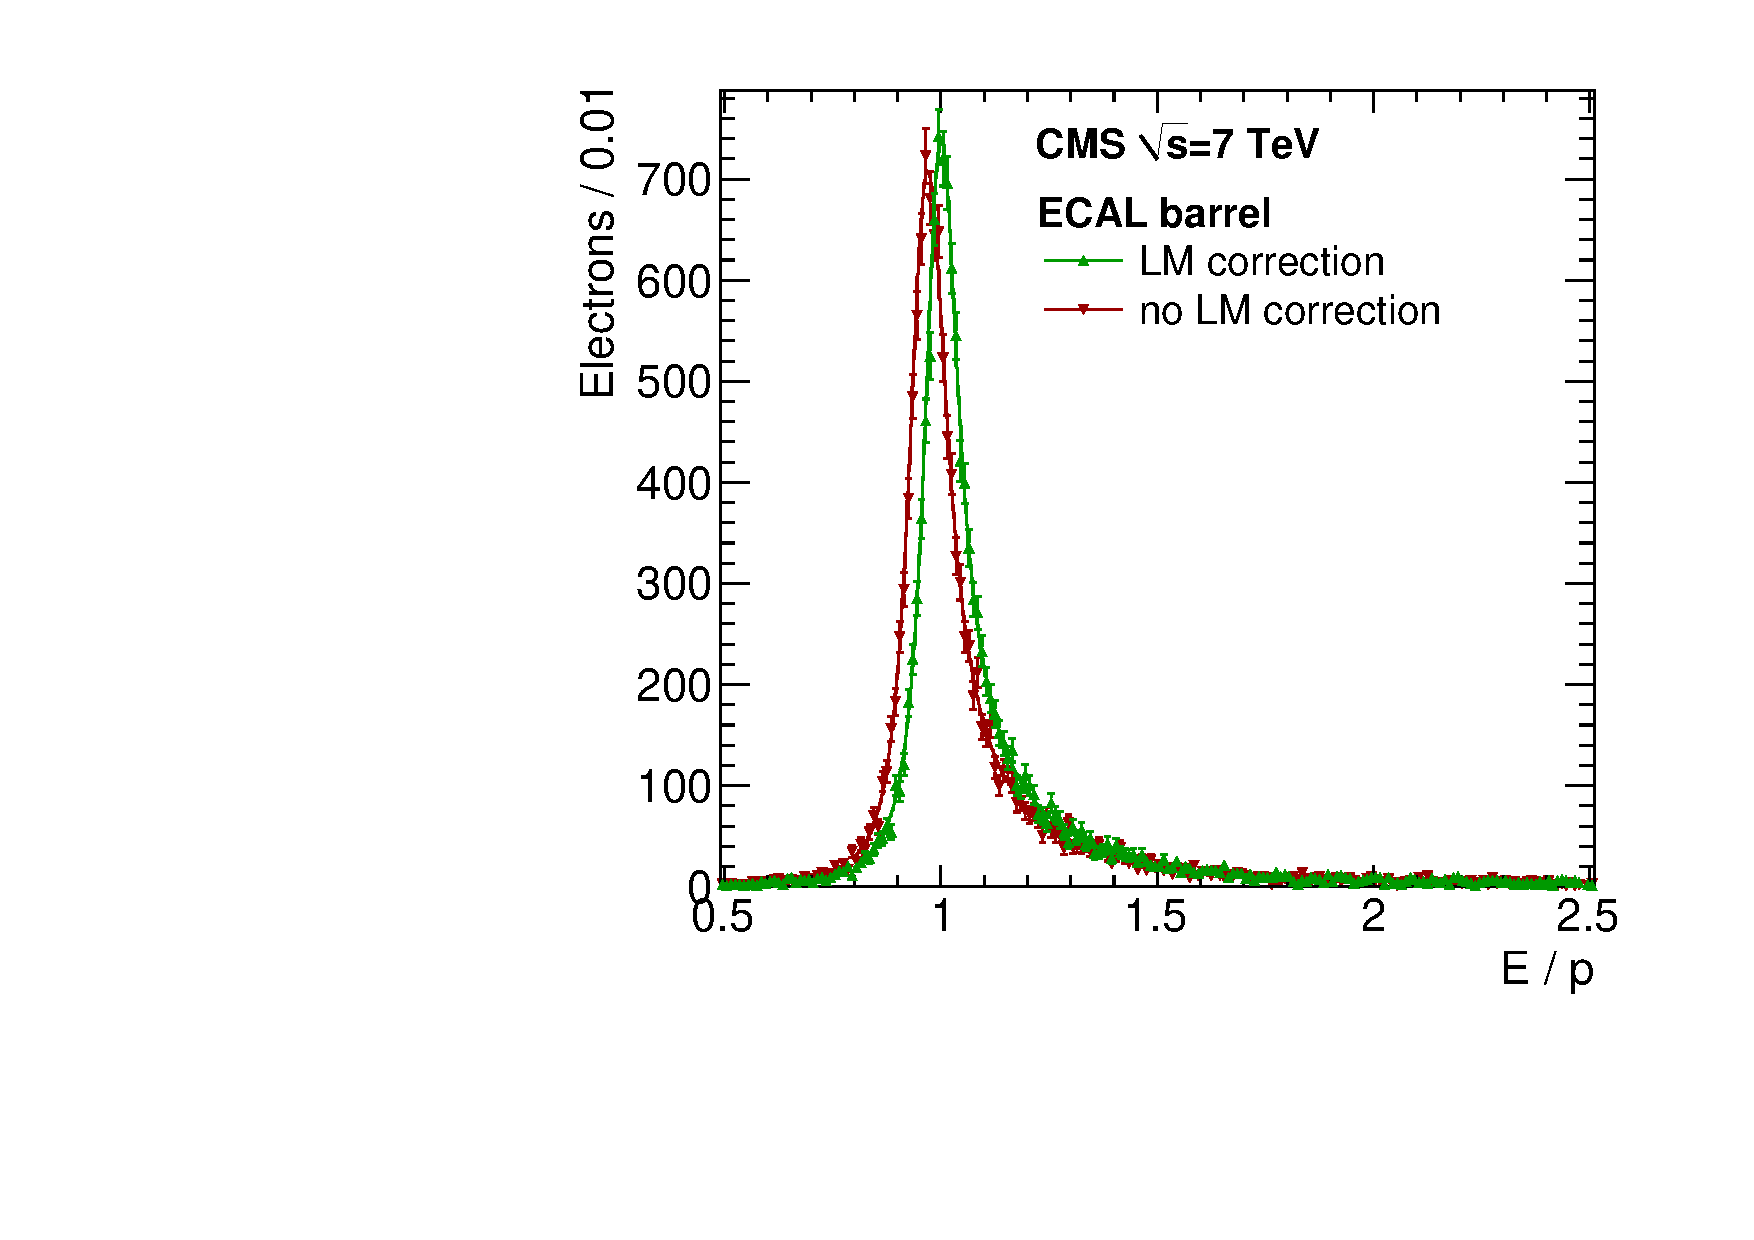
\includegraphics[width=0.40\linewidth]{figs/cms/EoP_TypicalFit_EB.pdf} &
 \hspace{-1cm}
 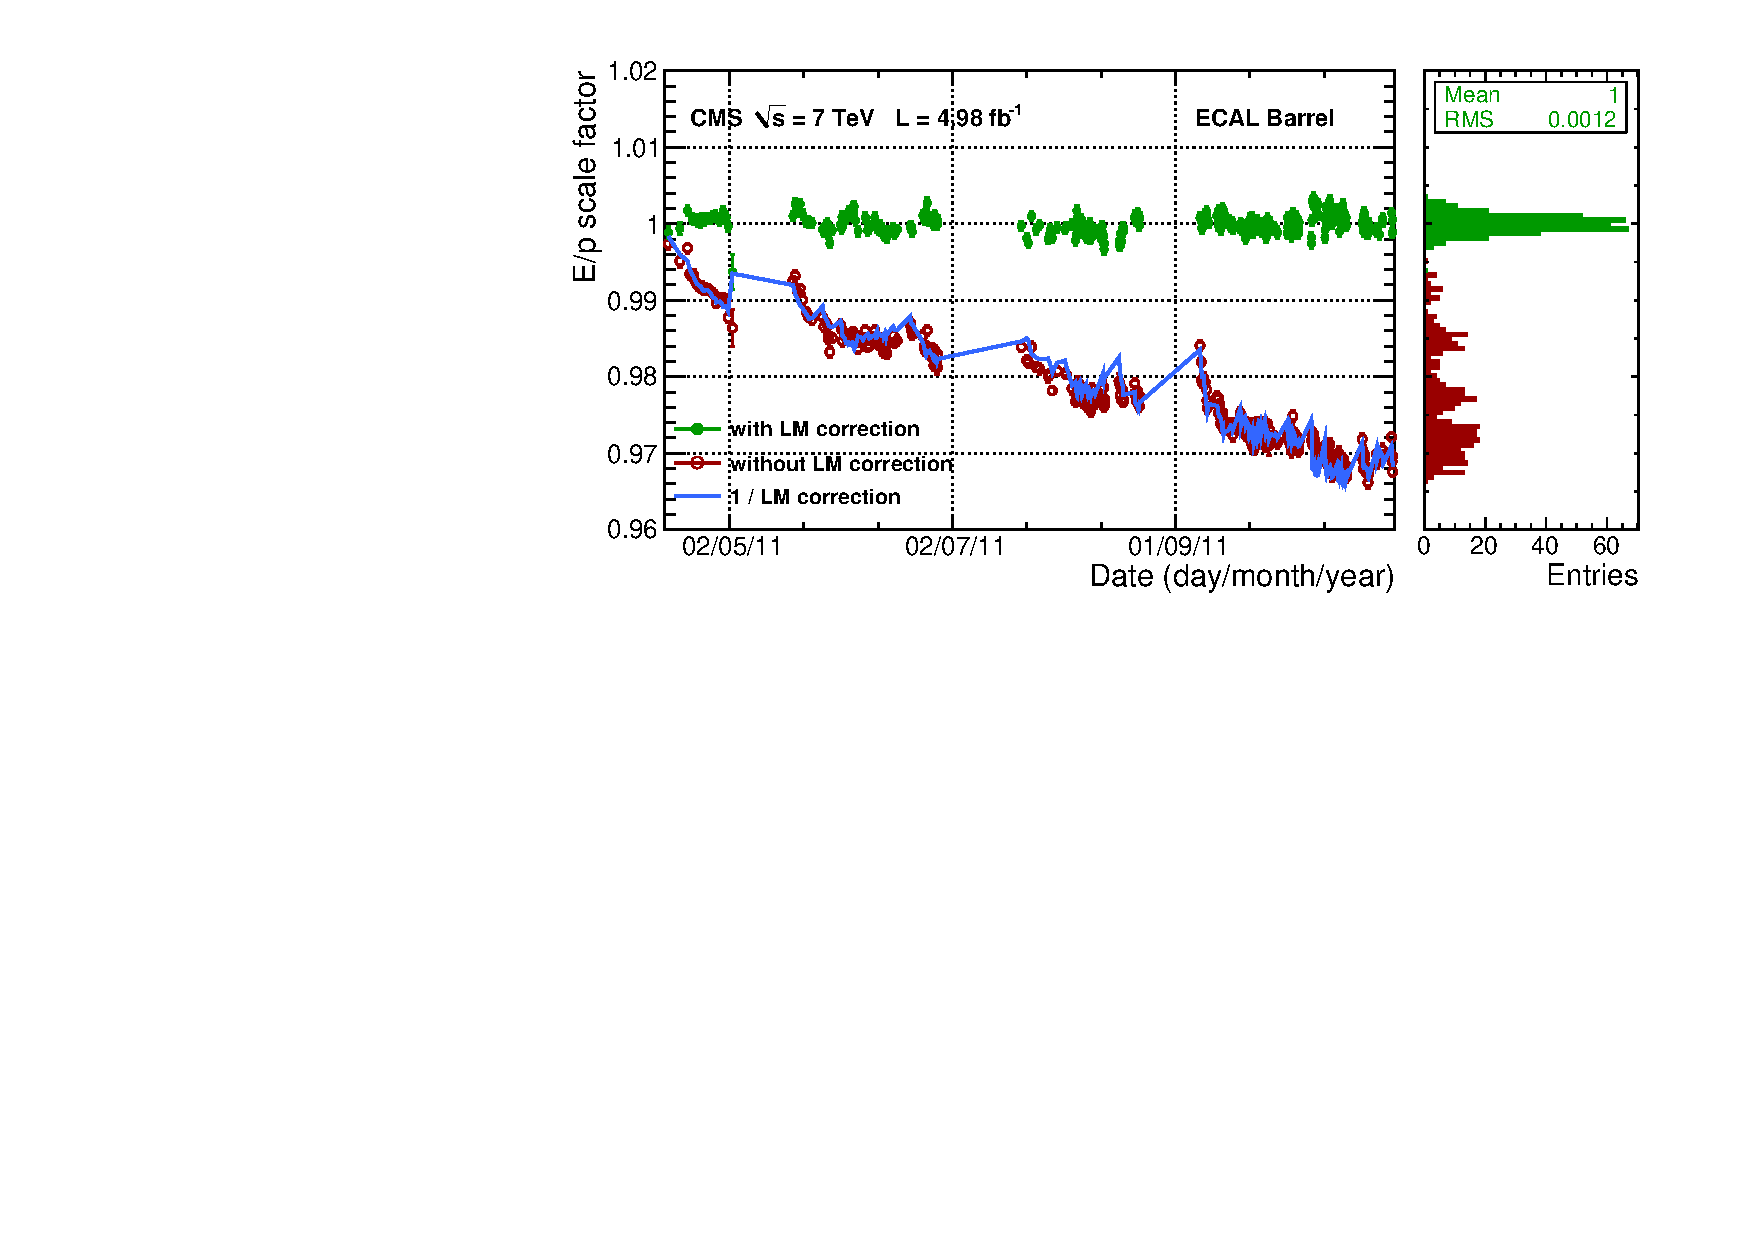
\includegraphics[width=0.69\linewidth]{figs/cms/EsuPhistoryEB.pdf} \\
 \hspace{-0.5cm}
 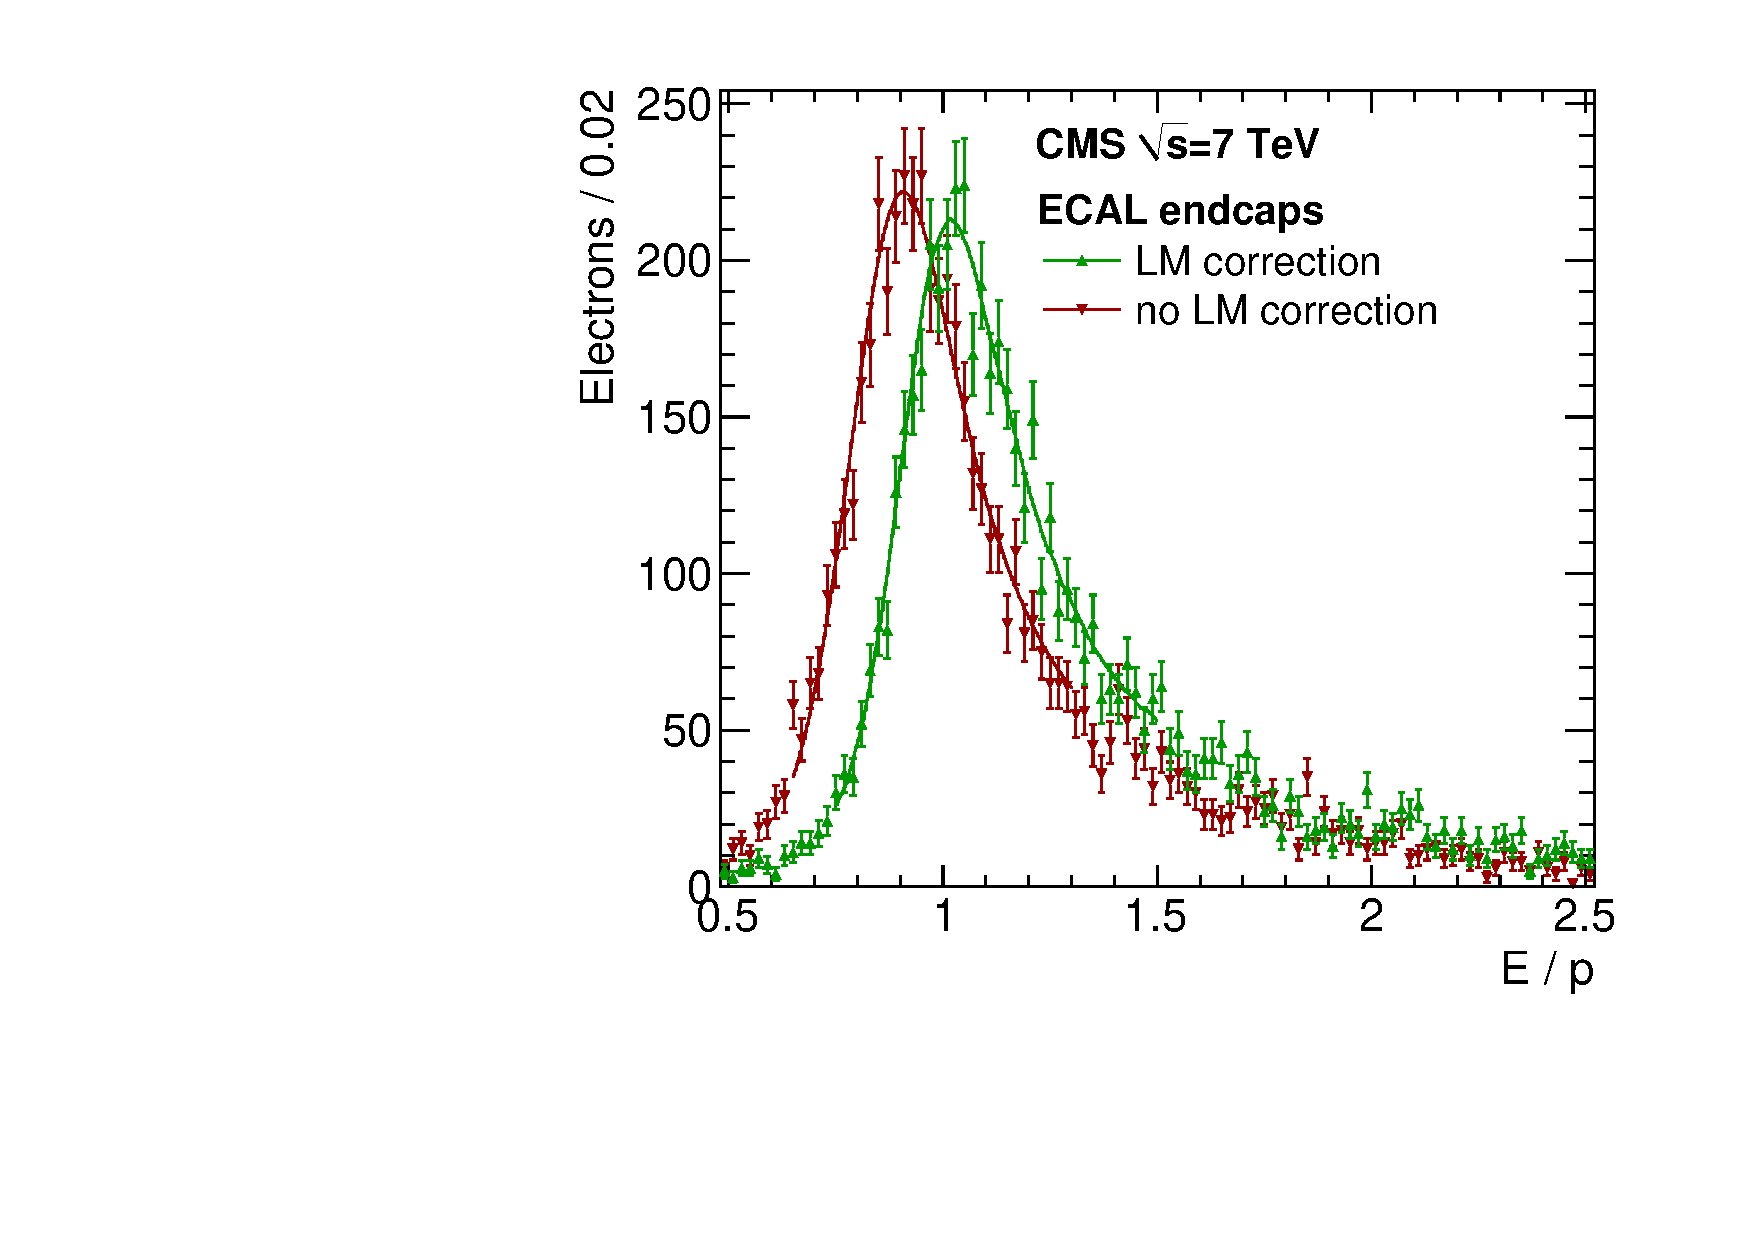
\includegraphics[width=0.40\linewidth]{figs/cms/EoP_TypicalFit_EE.pdf} &
 \hspace{-1cm}
 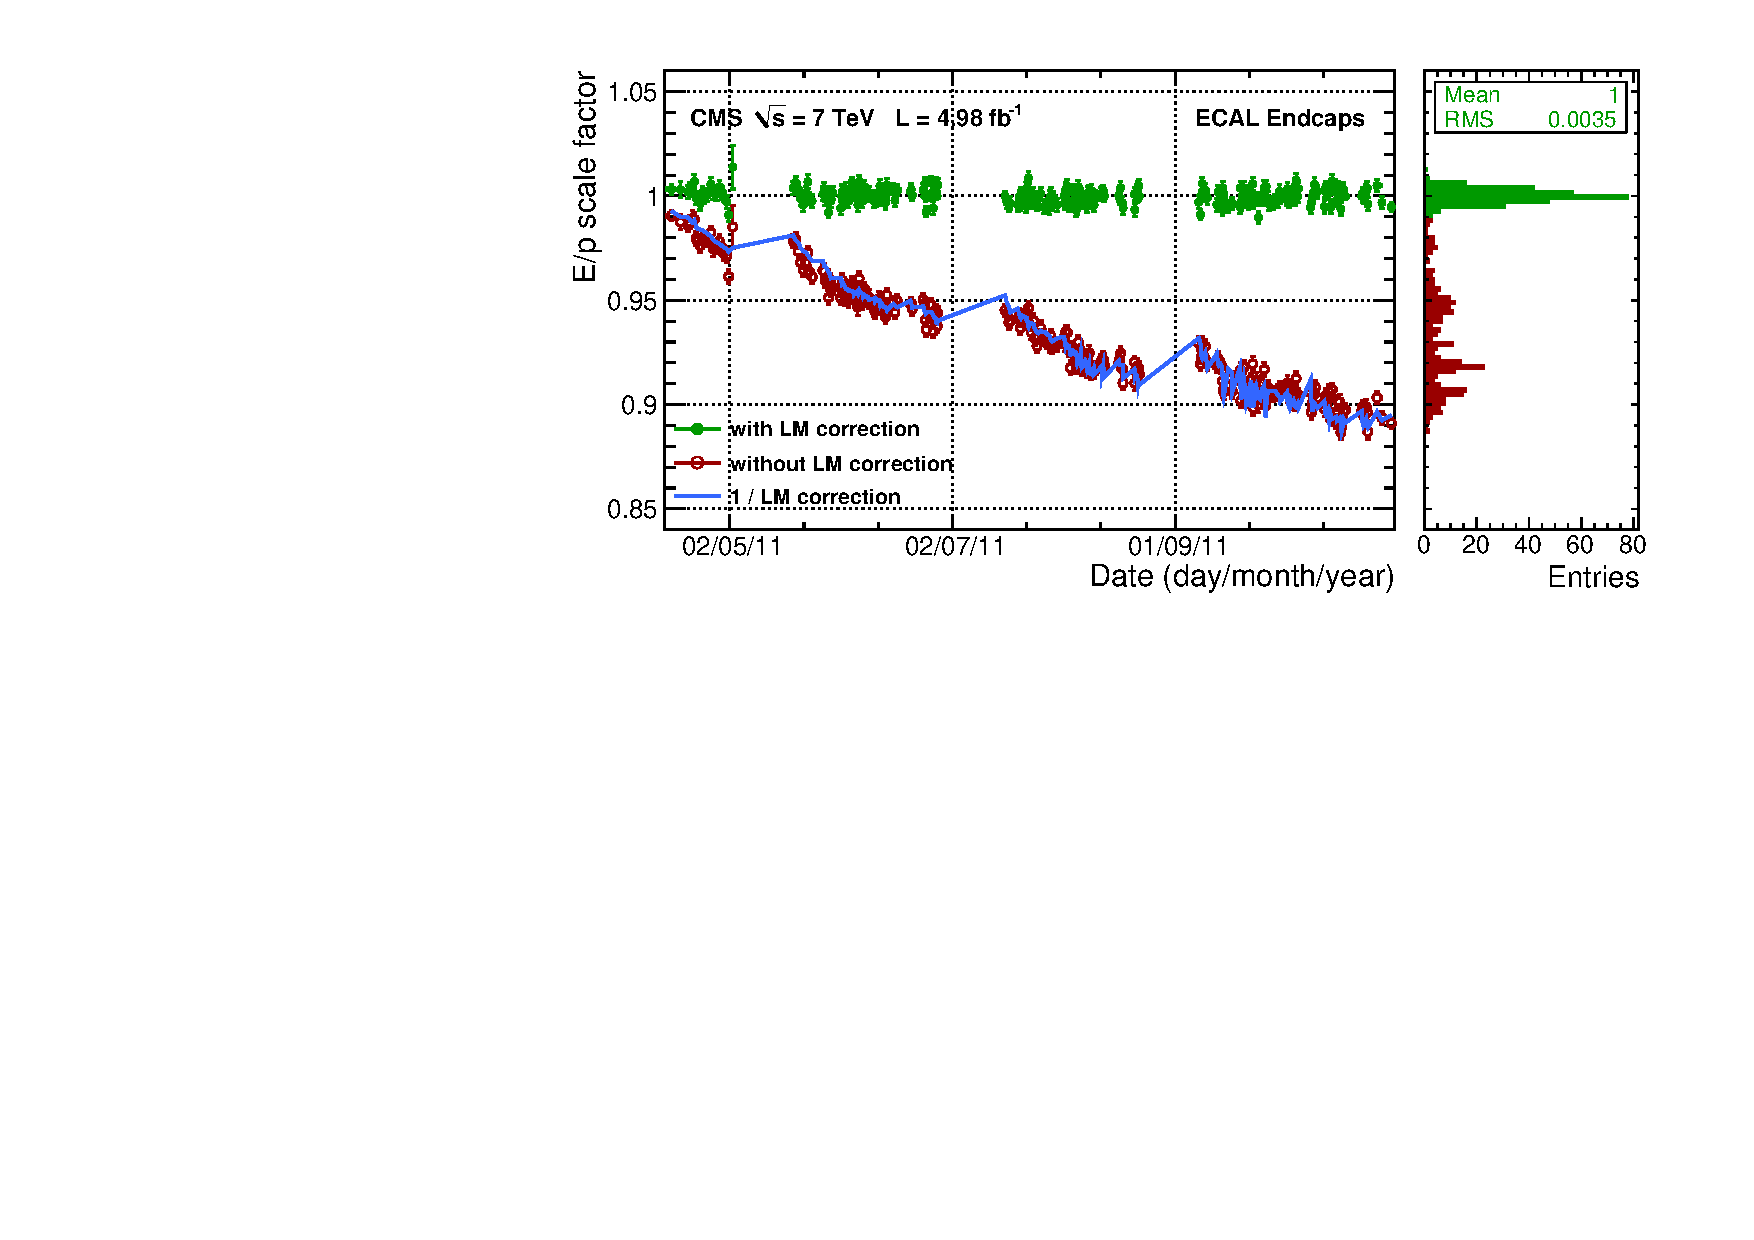
\includegraphics[width=0.69\linewidth]{figs/cms/EsuPhistoryEE_alpha116.pdf}
\end{tabular}
\end{center}
\caption{\label{fig:wenuEB}
Relative energy response variation for the barrel (top) and the endcaps (bottom)
determined from the $E/p$ analysis of electrons in $\PW$-boson decays.
Left: examples of fits to the $E/p$ distributions before (red) and
after (green) laser corrections. Middle: Response stability during the
2011 $\Pp\Pp$ data-taking period before (red open circles) and after
(green points) response corrections; the blue line shows the inverse
of the average laser corrections. Right: Distribution of the projected
relative energy scales.}
\end{figure}

\subsection{Data Scouting}
\label{sec:scouting}

An extension of the alignment/calibration data-taking strategy, referred to as \emph{data
  scouting}, is based on reducing the event size from the default of
$\sim 1$\unit{MB} in order to increase the recorded event rate and
thus increase physics signal acceptance. This
approach, first implemented at the LHC by the CMS experiment in
2011~\cite{CMS-DP-2012-022}, allows us to increase the physics signal
acceptance of CMS even in the presence of backgrounds with large cross
sections. This is particularly useful in the search for
narrow resonances in the dijet mass spectrum, as described in Ch.~\ref{ch:dijet}, where this strategy allows the search to
be extended into a low-dijet-mass region previously only accessible at
lower-energy colliders~\cite{Khachatryan:2016ecr,CMS-PAS-EXO-16-032}.

Fig~\ref{fig:DataScouting} schematically displays the $H_{\mathrm{T}}$
thresholds used for the different varieties of data scouting during the
2015 and 2016 runs and Fig~\ref{fig:DataScoutingContent} displays the
corresponding event content. \emph{Calo scouting}, which selects
events based only on Calo jets and records only calorimetric
information, has a very small event size of $\sim 1.5$\unit{kB}, allowing the
rate to go as a high as 3.8 \unit{kHz}. Meanwhile, \emph{PF scouting},
which runs the full PF algorithm and records all PF-reconstructed
information, including leptons, photons, and jets with \cPqb-tagging
information, has a larger event size $\sim 10$\unit{kB}. In order to stay within the
HLT timing budget, the maximum permissible rate is 720 \unit{Hz}. Simultaneously, the \emph{data parking} stream sends the
full raw events from PF scouting directly to tape without reconstruction. This
multifaceted approach is advantageous in the case that a signal is
seen in the scouting data that warrants more investigation.

\begin{figure}\centering
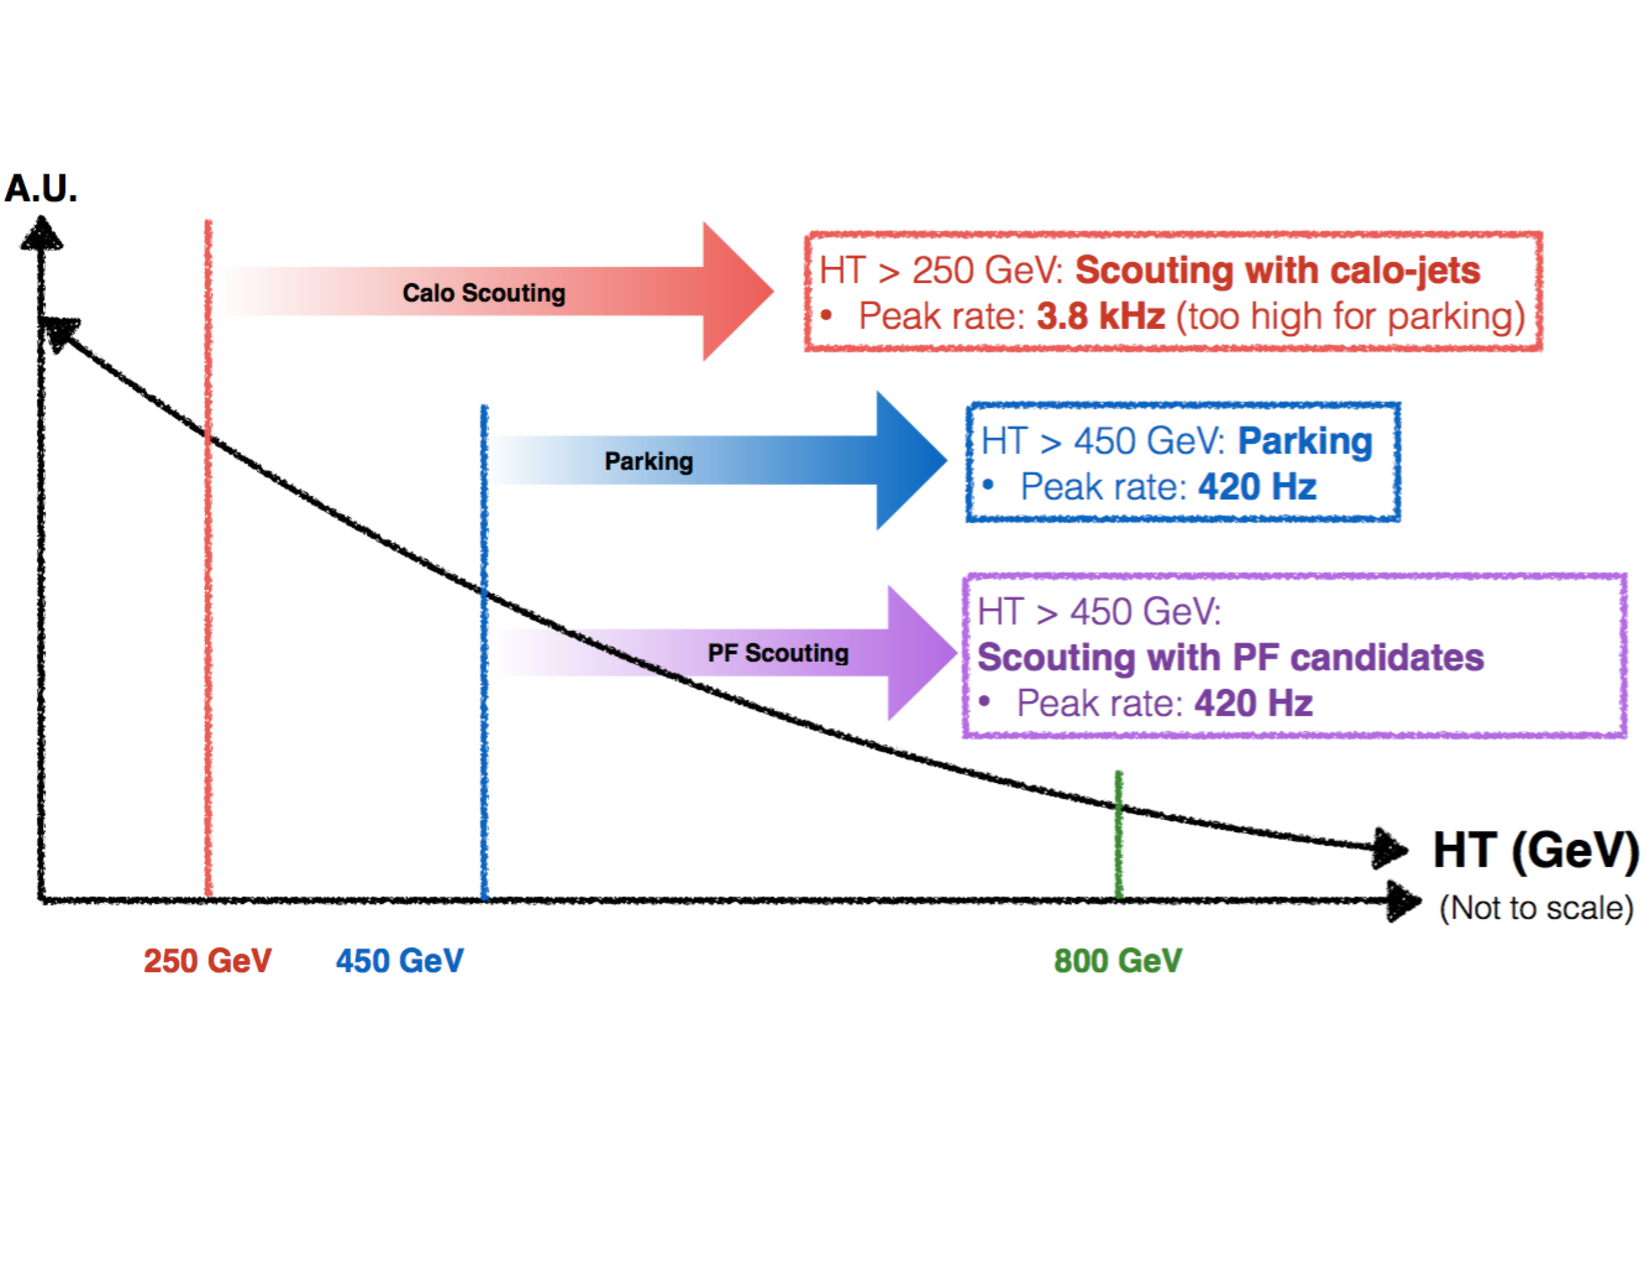
\includegraphics[width=.9\textwidth]{figs/cms/Scouting2015.pdf}\\
\includegraphics[width=.9\textwidth]{figs/cms/Scouting2016.pdf}
\caption{HLT $H_\mathrm{T}$ thresholds for Calo and PF scouting for
  2015 (top) and 2016 (bottom) data-taking runs. The
  rates for the 2015 (2016) are normalized to an instantaneous luminosity
  of $7\times 10^{33}$ cm$^{-2}$ s$^{-1}$ ($10^{34}$ cm$^{-2}$
  s$^{-1}$). \label{fig:DataScouting}}
\end{figure}

\begin{figure}\centering
\includegraphics[width=.45\textwidth]{figs/cms/pfscoutingeventcontent.png}
\includegraphics[width=.45\textwidth]{figs/cms/caloscoutingeventcontent.png}
\caption{The event content for PF scouting (left), which amounts to
  $\sim 10$\unit{kB}, and Calo scouting (right), which amounts to
  $\sim 1.5$\unit{kB}.\label{fig:DataScoutingContent}}
\end{figure}

\chapter{Topological HLT Development at $\sqrt{s}=13 \TeV$}
\label{ch:hlt13TeV}

To target a broad range of new physics possibilities, we designed four different
types of triggers for use at $\sqrt{s}=13\TeV$:
\begin{itemize}
\item Dijet razor trigger with hyperbolic \MR and \Rtwo requirements targetting the squark pair production topology;
\item Quadjet razor trigger with hyperbolic \MR and \Rtwo requirements
  targetting top-squark or gluino pair production topologies;
\item High-\Rtwo trigger targetting dijet+invisible topologies with
  large transverse momentum imbalance; and
\item Razor $\PH(\bbbar)$ trigger targetting production of
  $\PH(\bbbar)+\mathrm{jet}+\mathrm{invisible}$ with some transverse momentum imbalance.
\end{itemize}

The dijet and quadjet razor triggers are broadly motivated by SUSY pair
production and represent an update and incremental improvement of the razor triggers
used in previous searches at $\sqrt{s}=8\TeV$~\cite{razor8TeV}. Both
sets of triggers are based on hyperbolic thresholds in the $(\MR,\Rtwo)$
plane, with the 2015 updated thresholds shown in
Fig~\ref{fig:hyperbolic}. The 2015 hyperbolic contours follow the
iso-probability contours derived from the background-only fit to the MultiJet category
in the 8\TeV razor search performed using 2012 data. This implies
these hyperbolic contours efficiently reject background, while
maintaining a large acceptance for SUSY signal models with large
characteristic mass scale $M_{\Delta}\gtrsim 500 \GeV$ and sufficient
transverse momentum imbalance. Another update is that the 13 \TeV razor triggers are based on PF-reconstructed objects rather
than Calo jets and muons, which means the online $\Rtwo$ variable is
much more correlated with the offline $\Rtwo$ variable, which is also
PF-based. This leads to an improved trigger efficiency for 2015, shown
in Fig.~\ref{fig:turnons}.

\begin{figure}[htb!]
\centering
\includegraphics[width=0.49\textwidth]{figs/hlt13TeV/HLTRsqMR.pdf}
\caption{\label{fig:hyperbolic} Hyperbolic and baseline thresholds in
  \Rtwo and \MR used in the dijet and quadjet razor triggers.}
\end{figure}

\begin{figure}[ht!]
\centering
\includegraphics[width=0.45\textwidth]{figs/hlt13TeV/turnons_2015_no100GeVmuons/HLT_RsqMR240_Rsq0p09_MR200_HLT_RsqMR240_Rsq0p09_MR200_4jet_HLT_Rsq0p25_HLT_Ele27_eta2p1_WPLoose_Gsf_effRsq_MR500.pdf}
\includegraphics[width=0.45\textwidth]{figs/hlt13TeV/turnons_2015_no100GeVmuons/HLT_RsqMR240_Rsq0p09_MR200_HLT_RsqMR240_Rsq0p09_MR200_4jet_HLT_Rsq0p25_HLT_Ele27_eta2p1_WPLoose_Gsf_effMR_Rsq0p25.pdf}\\
\includegraphics[width=0.45\textwidth]{figs/hlt13TeV/turnons_2015_no100GeVmuons/HLT_RsqMR240_Rsq0p09_MR200_HLT_RsqMR240_Rsq0p09_MR200_4jet_HLT_Rsq0p25_HLT_Ele27_eta2p1_WPLoose_Gsf_eff2D.pdf}
\caption{\label{fig:turnons} Trigger efficiencies as measured using a
  data sample of single-electron events for $\Rtwo$ (top
  left), $\MR$ (top right), and in the $(\MR,\Rtwo)$ plane (bottom).}
\end{figure}

The high-\Rtwo trigger is motivated by the search for the direct
production of dark matter (DM) particles at the
LHC~\cite{Khachatryan:2016reg}.  DM particles themselves
would not leave a detectable signal in the detector, but if
they were produced in association with high-energy quarks or gluons,
they could produce signatures with jets and transverse
momentum imbalance. The traditional approach, employed by both CMS and
ATLAS, is to search in events with one high-$\pt$ jet and large $\MET$
(so-called monojet searches)~\cite{Aad:2011xw,Chatrchyan:2012me}. A complementary
approach is to search in events with at least two jets passing a looser
event selection using the razor variables. The sensitivity of these variables to direct DM production was
suggested in Ref.~\cite{Fox:2012ee}, and the search carried out by CMS
demonstrates that the resulting sensitivity is comparable to that of
monojet searches~\cite{Fox:2012ee,Papucci:2014iwa,Khachatryan:2016reg}.
The hallmark of many direct DM production models in the razor plane is an
almost-peaking behavior near $\Rtwo\gtrsim 0.8$ and an exponentially
falling $\MR$ distribution with no special structure. For this reason,
the high-\Rtwo trigger is designed with a threshold in \Rtwo but no
requirement on \MR to allow for greater DM signal acceptance.

Finally, the razor $\PH(\bbbar)$ trigger is motivated by an
excess observed by CMS in events with a $\PH
(\Pgg\Pgg)$ plus at least one extra jet~\cite{RazorHgaga}. The excess,
corresponding to a local significance of
$2.9\sigma$, consists of five events observed with $400\GeV<\MR<1400
\GeV$,  $\Rtwo>0.05$, and $m_{\Pgg\Pgg}$ consisent with $m_{h^0}= 125
\GeV$ in a high-resolution diphoton category, compared to less than one
expected background event. The general idea is to search for a similar
signature in the $\PH\to\bbbar$ channel, which comes with a larger
signal yield (90,000 times more assuming SM Higgs branching ratios),
but a much larger background, resulting in a considerably worse
signal-to-background ratio. To this end, the trigger
requirements of three jets, two \cPqb-jets, $\MR>300
\GeV$,  $\Rtwo>0.02$, and $m_{\bbbar}$ roughly consisent with $m_{h^0}= 125
\GeV$ are chosen to (a) maintain signal acceptance based on the observed
features, (b) accept additional events outside of $m_{h^0}$ window
to permit a robust background estimation based on a fit, and (c)
limit the rate and average CPU time of the trigger to an acceptable level.
%, reduced to $1.6\sigma$ after the LEE.

\section{HLT Path Design}

The design of the four main HLT paths in terms of producers (in
purple) and filters (in blue) is shown
in Fig.~\ref{fig:HLTdesign}. The first step is always a filter, which
rejects events with no hadronic activity above a certain threshold reconstructed by the L1 trigger.
As detailed in Sec.~\ref{sec:trigger}, there are two main technical
constraints an HLT path must satisfy: (a) the average CPU time required must be
small enough so that the entire HLT menu fits within the timing budget
 of $\sim160$ \unit{ms} and (b) the rate must
be small enough so that the entire HLT menu fits within the maximum
allowable rate  of $\sim1$ \unit{kHz}. To satisfy the timing
requirement, all the paths are outfitted with
calorimetric prefilters. The aim of these prefilters is to reject
events based only on information from the calorimeters, whose
reconstruction algorithms are much faster than the PF algorithm. In
other words, to keep the timing of the paths manageable, it is
necessary to limit the input rate to the PF algorithm. Thus, all four
triggers have prefilter based on calorimeter-based versions of the razor
variables.

\begin{figure}[ht!]
\centering
\includegraphics[width=0.8\textwidth,clip=true,viewport=0 110 1024
500]{figs/hlt13TeV/HLTDijetDesign.pdf}\\
(a) HLT\_RsqMR240\_Rsq0p09\_MR200 \\
\includegraphics[width=0.8\textwidth,clip=true,viewport=0 110 1024
500]{figs/hlt13TeV/HLTQuadjetDesign.pdf}\\
(b) HLT\_RsqMR240\_Rsq0p09\_MR200\_4jet \\
\includegraphics[width=0.8\textwidth,clip=true,viewport=0 220 1024
500]{figs/hlt13TeV/HLTR2Design.pdf}\\
(c) HLT\_Rsq0p25\\
\includegraphics[width=0.8\textwidth,clip=true,viewport=0 110 1024
500]{figs/hlt13TeV/HLTRazorHbbDesign.pdf}\\
(d) HLT\_Rsq0p02\_MR300\_TriPFJet80\_60\_40\_\\
~DoublePFBTagCSV0p7\_0p4\_Mbb60\_200
\caption{\label{fig:HLTdesign} Flow of the producer steps (in purple)
  and filter steps (in blue) in
  the razor triggers.}
\end{figure}

\section{HLT Rate and Average CPU Time}

The HLT rates and average CPU time consumed for the razor triggers, as measured in data
collected in 2015, are presented in Tab.~\ref{tab:rates2015}.

%\begin{table*}[ht!]
%\centering
% \caption{Rates for 0\unit{T} triggers.
% \label{tab:rates0T}}
%\resizebox{\textwidth}{!}{
%\begin{tabular}{l|l|l}
%\multirow{2}{*}{Trigger path} &  Data rate (run 260039) & MC rate (Spring '15) \\
% &  $4\times 10^{33}$ \unit{cm$^{-2}$ s$^{-1}$}, 17 PU &  \\\hline
%HLT\_Rsq0p25\_Calo & 3.7 Hz & \\
%HLT\_RsqMR240\_Rsq0p09\_MR200\_4jet\_Calo & 5.6 Hz & \\
%HLT\_RsqMR240\_Rsq0p09\_MR200\_Calo & 18.2 Hz & 
%\end{tabular}}
%\end{table*}

\begin{table*}[ht!]
\centering
 \caption{HLT rates and average CPU time consumed for the razor
   triggers under different running conditions in 2015. Run 260627 had peak $5\times 10^{33}$ cm$^{-2}$
   s$^{-1}$ peak instantaneous luminosity with 17 average pileup
   interactions, while run 259721 had $1.5\times 10^{33}$ cm$^{-2}$
   s$^{-1}$ peak instananeous luminosity with 23 average pileup interactions. \label{tab:rates2015}}
\resizebox{\textwidth}{!}{
\begin{tabular}{l|l|l}
\multirow{2}{*}{Trigger path} &  Data rate (run 260627) & CPU time (run 259721) \\
 &  $5\times 10^{33}$ cm$^{-2}$ s$^{-1}$, 17 PU &  $1.5\times 10^{33}$ cm$^{-2}$ s$^{-1}$, 23 PU \\\hline
HLT\_RsqMR240\_Rsq0p09\_MR200 & 7.7 Hz & 27 \unit{ms}\\ 
HLT\_RsqMR270\_Rsq0p09\_MR200 & 2.3 Hz & 17 \unit{ms} \\ 
HLT\_RsqMR240\_Rsq0p09\_MR200\_4jet & 1.2 Hz & 20 \unit{ms}\\
HLT\_RsqMR270\_Rsq0p09\_MR200\_4jet & 0.5 Hz  & 15 \unit{ms} \\
HLT\_Rsq0p25 & 0.7 Hz & 14 \unit{ms}\\
HLT\_Rsq0p30 & 0.4 Hz & 14 \unit{ms} \\
HLT\_Rsq0p02\_MR300\_TriPFJet80\_60\_40\_&\multirow{2}{*}{16.0 \unit{Hz}} & \multirow{2}{*}{34 \unit{ms}}\\
~DoublePFBTagCSV0p7\_0p4\_Mbb60\_200 & &\\
HLT\_Rsq0p02\_MR300\_TriPFJet80\_60\_40\_ & \multirow{2}{*}{8.0 Hz} & \multirow{2}{*}{26 \unit{ms}}\\
~DoublePFBTagCSV0p7\_Mbb60\_200 & & 
\end{tabular}}
\end{table*}
% timing from: 
% https://docs.google.com/spreadsheets/d/1qu0dKZfjHEl073QyXayxzPBNoT10GZKMiPU9-z8VSeU/edit#gid=0
% supplemented by my measurement (for RsqMR240...)
% https://www.dropbox.com/s/z8qfx57du7h3gzq/TSG_RazorHLT2016_30Mar2016.pdf?dl=0


\section{Pileup Dependence}

The HLT rate, normalized by the number of collinding bunches, as a function of the number of pileup interactions for
each razor trigger and for different data runs collected in 2015 is
shown in Fig.~\ref{fig:HLTpileup}. Nominally, the dependence of the
normalized HLT rate on pileup is expected to be linear, as is the case
for single-object triggers. Contrastingly, triggers based on``sum'' quantities
(such as $H_\mathrm{T}$ or $\MET$) and multi-object triggers often
demonstrate a nonlinear dependence on pileup~\cite{Bocci:2016}. As the
razor triggers are both based on sum quantities and multiple objects,
they also exhibit some nonlinear dependence on pileup. This implies
that as the pileup increases at the LHC in 2016 and beyond, either trigger thresholds
will need to rise dramatically or more sophisticated methods to deal
with pileup contamination will need to implemented. One such method is
delineated in Ch.~\ref{ch:timing}.

\begin{figure}[ht!]
\begin{tabular}{cc}
\centering 
\includegraphics[width=0.49\textwidth]{figs/hlt13TeV/linear/HLT_RsqMR240_Rsq0p09_MR200_instLumi_vs_rawRate.pdf}
  & \includegraphics[width=0.49\textwidth]{figs/hlt13TeV/linear/HLT_RsqMR240_Rsq0p09_MR200_4jet_instLumi_vs_rawRate.pdf}\\
(a) HLT\_RsqMR240\_Rsq0p09\_MR200 & (b) HLT\_RsqMR240\_Rsq0p09\_MR200\_4jet\\
\includegraphics[width=0.49\textwidth]{figs/hlt13TeV/linear/HLT_Rsq0p25_instLumi_vs_rawRate.pdf}
  &\includegraphics[width=0.49\textwidth]{figs/hlt13TeV/linear/HLT_Rsq0p02_MR300_TriPFJet80_60_40_DoublePFBTagCSV0p7_0p4_Mbb60_200_instLumi_vs_rawRate.pdf}\\
\multirow{2}{*}{(c) HLT\_Rsq0p25} & (d) HLT\_Rsq0p02\_MR300\_TriPFJet80\_60\_40\_\\
& ~DoublePFBTagCSV0p7\_0p4\_Mbb60\_200
\end{tabular}
\caption{\label{fig:HLTpileup} Pileup dependence of the razor triggers.}
\end{figure}



\part{Searches for new physics at the LHC}
\label{part:searches}
\chapter{Searches for Supersymmetry at $\sqrt{s}=8\TeV$}
\label{ch:analysis8TeV}

As discussed in Sec.~\ref{sec:sms}, models of SUSY predict
additional, undiscovered fundamental particles which correspond to the
heavy superpartners of SM particles. Of particular interest is the production of top squarks, bottom squarks, and gluinos due to their role in taming
the quadric divergence of the Higgs mass in the SM (see
Sec.~\ref{sec:susynaturalness}). The residual fine-tuning inherent in these models is
dependent on the masses of these superpartners, with a
preference for smaller masses to avoid large fine-tuning. These
considerations have motivated searches for the lightest allowed top
and bottom squarks, as well as gluinos that may that couple to top/bottom
squarks, whose decays would produce final states enriched in
\PQb-jets. Moreover, due to the possible presence of top quarks that
produce leptons $\sim30\%$ of the time in the
decay chain, electrons or muons may be used the event selection to
enhance the signal-to-background ratio. We exploit both of
these features (\PQb-jets and leptons) in the event classification.

We classify events into different ``boxes,'' or data categories, based on
the jet multiplicity, \PQb-jet multiplicity, and lepton (\Pe or \Pgm)
multiplicity. The advantages of this classification are (i) by
isolating different SM background processes, like $\ttbar$, we can better
model them individually, and (ii) in the event of a discovery, we may be
able to infer the values of certain SUSY branching fractions based on the boxes where
the signal is present. The likelihood functions of the different boxes are
statistically combined to exclude or discover particular SUSY
models. In the following, this classification and statistical
combination is referred to as the razor box approach.

In this chapter, we present an inclusive search for gluinos and top
squarks\footnote{Though we don't explicitly interpret our results
  in the context of bottom squark production, many of the conclusions regarding top squark
  production carry over.} using $\Pp\Pp$ collision data collected by CMS at $\sqrt{s}=8\TeV$ in the
context of the minimal natural SUSY spectrum outlined in
Sec.~\ref{sec:sms}~\cite{razor8TeV}. Previous searches for natural SUSY by CMS~\cite{1LepMVA,SUS12024,Chatrchyan:2014lfa,Chatrchyan:2013iqa,Chatrchyan:2013fea}
and ATLAS~\cite{Aad:2013wta,Aad:2014lra,Aad:2014pda,Aad:2014bva,Aad:2014qaa}
at $\sqrt{s}=7\TeV$ and $8\TeV$ have probed gluino masses up to 1300\GeV and top squark
masses up to 700\GeV under the assumptions of specific decay modes for
the SUSY particles. One important feature that sets this search apart
is that the SUSY parameter space of gluino and top squark branching ratios is
explored for the first time at the LHC~\cite{razor8TeV}. Notably, the
razor box approach ensures good sensitivity to a wide range of
branching ratios. In addition, we combine the results from the hadronic razor search
with those from a previous search~\cite{1LepMVA} for top-squark
production in the single-lepton (\Pe or \Pgm) channel to obtain
an improved bound on top-squark pair production. 

The remainder of this chapter is organized as follows. The event
selection and box definitions are detailed in
Sections~\ref{sec:selection8TeV}~and~\ref{sec:box8TeV},
respectively. The modeling of the SM backgrounds through a fit using
an emprical function is explained in Sec.~\ref{sec:bmodel8TeV}. In
particular, the motivation for this empirical function and the
properties that make it a suitable description are examined in Sec.~\ref{sec:function8TeV}.
The results of the fits to data are presented and compared to the
corresponding results in a signal injection scenario in
Sec.~\ref{sec:fit8TeV}. Finally, limits are derived in the context of the
natural SUSY scenario of Sec.~\ref{sec:sms}  and a summary is given in
Sections~\ref{sec:limit8TeV}~and~\ref{sec:conclusion8TeV},
respectively.

\section{Event selection}
\label{sec:selection8TeV}
Events are selected at the L1 trigger level by requiring at least two
jets with $|\eta|<3$. At the HLT level, events are selected using
dedicated razor algorithms, consisting of a loose selection on \MR and
$\Rtwo$. Razor-specific triggers, similar to those discussed in
Ch.~\ref{ch:hlt13TeV}, are used in the HLT in order to avoid
biases on the shapes of distributions from the SM background that are
introduced by requirements on more traditional selection variables
such as $\ETm$.  The razor triggers reject the majority of the SM
background, which mostly appears at low $\Rtwo$ and low $\MR$, while
retaining events in the signal-sensitive regions of the ($\MR$,
$\Rtwo$) plane. Two types of triggers are used: i) a hadronic razor
trigger, which selects events that contain at least two jets with
transverse momentum $\pt>64\GeV$ by applying threshold requirements on
$\Rtwo$, $\MR$, and their product; ii) a muon and electron razor
trigger, which selects events with at least one isolated electron or
muon with $\pt>12\GeV$ in combination with looser requirements on
$\Rtwo$, $\MR$, and their product. The trigger efficiency, evaluated
using a dedicated trigger, is measured to be $(95 \pm 5)\%$ and is
independent of $\Rtwo$ and $\MR$ for the events selected with the
baseline requirements described in Sec.~\ref{sec:kinematic}.

Following the trigger selection, events are required to contain at
least one reconstructed interaction vertex. If more than one vertex is
found, the one with the highest $\pt^2$ sum of associated tracks is
chosen as the interaction point for event reconstruction. Algorithms are
used to remove events with detector- and beam-related noise that can
mimic event topologies with high energy and large $\pt$
imbalance~\cite{Chatrchyan:2011tn,Chatrchyan:2012lia,Khachatryan:2014gga}.

The analysis uses a global event description based on the CMS particle
flow (PF) algorithm~\cite{PF1,PF2}, described in Sec.~\ref{sec:pf}.
% Individual particles (PF candidates) are reconstructed by combining the information from the inner
%tracker, the calorimeters, and the muon system. Five categories of PF
%candidates are defined: muons, electrons, photons (including their
%conversions to $\Pep\Pem$ pairs), charged hadrons, and neutral
%hadrons. The contamination from other proton-proton collisions in the
%same or in neighboring bunch crossings is reduced by discarding the
%charged PF candidates not compatible with the interaction point. When
%computing lepton isolation and jet energy, the corresponding
%contamination from neutral particles is subtracted on average by
%applying an event-by-event correction based on the jet-area
%method~\cite{jetarea_fastjet,jetarea_fastjet_pu,JME-JINST}.

A ``tight'' lepton identification is used for muons and electrons,
consisting of requirements on isolation and track reconstruction
quality. For electrons, the shape and position of the energy deposit
in the electromagnetic calorimeter is used to further reduce the contamination from
hadrons~\cite{Chatrchyan:2013iaa}. For events with one identified
tight lepton, additional muons or electrons are identified through a
``loose'' lepton selection, characterized by a relaxed isolation
requirement~\cite{Chatrchyan:2013mxa}. Tight leptons are
required to have $\pt>15$\GeV and loose leptons $\pt>10$\GeV.

Jets are reconstructed by clustering the PF candidates with the
\textsc{FastJet}~\cite{fastjet} implementation of the anti-\kt~\cite{antikt} algorithm with the distance parameter $R=0.5$. We
select events containing at least two jets with $\pt>80$\GeV and
$\abs{\eta}<2.4$, representing a tighter version of the L1 jet selection criterion. The $\pt$
imbalance in the event, $\ptvecmiss$, is the
negative of the sum of the $\ptvec$ of the PF candidates in the
event. Its magnitude is referred to as $\ETm$. For each event, the $\ptvecmiss$ and the
four-momenta of all the jets with $\pt>40$\GeV and $\abs{\eta}<2.4$ are
used to compute the razor variables, as described in section~\ref{sec:kinematic}.

The medium working point of the combined secondary vertex
algorithm~\cite{btag8TeV}, describred in Sec.~\ref{sec:btag}, is used for \PQb-jet tagging. The \PQb-tagging
efficiency and mistag probability are measured from data control
samples as a function of the jet $\pt$ and $\eta$. Correction factors
are derived for Monte Carlo (MC) simulations through comparison of the
measured and simulated \PQb-tagging efficiencies and mistag rates found
in these control samples~\cite{btag8TeV}.

Events with no \PQb-tagged jet are discarded, a criterion motivated by
the natural SUSY signatures described in Sec.~\ref{sec:sms}. A tighter
requirement ($\geq$2 \PQb-tagged jets) is imposed on events without an
identified tight lepton and fewer than four jets. This requirement reduces the
expected background from SM production of $\cPZ(\to\nu\bar\nu)+$jets
events to a negligible level.


\section{Box definitions}
\label{sec:box8TeV}

The selected events are categorized into the different razor boxes according to
their event content as shown in Tab.~\ref{tab:boxDef}. In the table,
the boxes are listed according to the filling order, from the first
(at the top of the table) to the last (at the bottom). If an event
satisfies the requirements of two or more boxes, the event is assigned
to the first listed box to ensure the boxes correspond to disjoint samples.

The events in the single-lepton and two-lepton boxes are recorded
using the electron and muon razor trigger. The remaining two boxes, generically
referred to as ``hadronic'' boxes, contain events recorded using the
hadronic razor trigger.

In the two-lepton boxes, the ($\MR$, $\Rtwo$)
distribution of events with at least one \PQb-tagged jet is studied. For
the other boxes, the data are binned according to the \PQb-tagged jet
multiplicity: 1 \PQb-tag, 2 \PQb-tags, and $\geq$3 \PQb-tags.

\begin{table*}[ht!]
\centering
 \caption{Kinematic and multiplicity requirements defining the nine
 razor boxes. Boxes are listed in order of event filling priority.
 \label{tab:boxDef}}
\resizebox{\textwidth}{!}{
\begin{tabular}{l|c|c|c|c}
\hline\hline
Box & Lepton & \PQb-tag & Kinematic & Jet \\
\hline
 \multicolumn{5}{c}{Two-lepton boxes}\\
\hline
\multirow{2}{*}{MuEle} & $\geq$1 tight electron and & \multirow{6}{*}{$\geq$1 \PQb-tag} & \multirow{2}{*}{} & \multirow{6}{*}{$\geq$2 jets}\\
& $\geq$1 loose muon & & & \\
%\cline{1-2}
\multirow{2}{*}{MuMu} & $\geq$1 tight muon and & & ($\MR >300$\GeV and $\Rtwo > 0.15$) and & \\
& $\geq$1 loose muon & & ($\MR > 350$\GeV  or $\Rtwo > 0.2$) & \\
%\cline{1-2}
\multirow{2}{*}{EleEle} & $\geq$1 tight electron and & & & \\
& $\geq$1 loose electron& & & \\
\hline
\multicolumn{5}{c}{Single-lepton boxes}\\
\hline
MuMultiJet & 1 tight muon & \multirow{4}{*}{$\geq$1 \PQb-tag} & & \multirow{2}{*}{$\geq$4 jets} \\
%\cline{1-2}
EleMultiJet &1 tight electron & & ($\MR > 300$\GeV and $\Rtwo > 0.15$) and & \\
%\cline{1-2}
%\cline{5-5}
MuJet & 1 tight muon & & ($\MR > 350$\GeV or $\Rtwo > 0.2$) & \multirow{2}{*}{2 or 3 jets}\\
%\cline{1-2}
EleJet & 1 tight electron & & &  \\
\hline
\multicolumn{5}{c}{Hadronic boxes}\\
\hline
MultiJet & none & $\geq$1 \PQb-tag & ($\MR > 400$\GeV and $\Rtwo > 0.25$) and &$\geq$4 jets\\
%\cline{1-3}
%\cline{5-5}
$\geq$2 \PQb-tagged jet & none & $\geq$2 \PQb-tag &  ($\MR > 450$\GeV
or $\Rtwo > 0.3$) & 2 or 3 jets\\
\hline\hline
\end{tabular}}
\end{table*}

A baseline kinematic requirement is applied to define the region in
which we search for a signal:
\begin{itemize}
\item $\MR>400$\GeV and $\Rtwo>0.25$ for the hadronic boxes;
\item $\MR>300$\GeV and $\Rtwo>0.15$ for the other boxes.
\end{itemize}
The tighter baseline selection for the hadronic boxes is a consequence
of the tighter threshold used for the hadronic razor trigger. The
kinematic plane defined by the baseline selection is divided into three
regions (see Fig.~\ref{fig:regions}):
\begin{itemize}
\item Low \MR sideband: $400<\MR<550$\GeV
 and $\Rtwo>0.30$ for the hadronic boxes;
 $300<\MR<450$\GeV and $\Rtwo>0.20$ for the other
 boxes.
\item Low  \Rtwo sideband: $\MR>450$\GeV and
  $0.25<\Rtwo<0.30$ for the hadronic boxes;
  $\MR>350$\GeV and $0.15<\Rtwo<0.20$ for the other
  boxes.
\item Signal-sensitive region: $\MR>550$\GeV and
 $\Rtwo>0.30$ for the hadronic boxes; $\MR>450$\GeV
 and $\Rtwo>0.20$ for the other boxes.
\end{itemize}
The bottom left corner of the razor plane, not included in any of the
three regions, is excluded from the analysis. Given this selection,
the multijet background from quantum chromodynamics processes is
reduced to a negligible level due to the fact that these processes
typically peak at $\Rtwo\approx0$ and fall exponentially for
larger values of $\Rtwo$~\cite{razorPRL,razorPRD}.

\begin{figure}[ht!]
\centering
\includegraphics[width=0.49\textwidth]{figs/analysis8TeV/SidebandL_MultiJet.pdf}
\includegraphics[width=0.49\textwidth]{figs/analysis8TeV/SidebandL_Mu.pdf}
\caption{\label{fig:regions} Definition of the sideband and the
 signal-sensitive regions used in the analysis, for (left) the hadronic
 boxes and (right) the other boxes.}
\end{figure}

\section{Background Modeling}
\label{sec:bmodel8TeV}
Under the hypothesis of no contribution from new-physics processes,
the event distribution in the considered portion of the
($\MR$, $\Rtwo$) plane can be described by the sum of
the contributions from SM $\cPV$+jets events (where
$\cPV$ indicates a $\PW$ or $\cPZ$ boson) and SM top quark-antiquark and
single-top events, where the events with a top quark are generically
referred to as the $\ttbar$ contribution. Based on MC studies, the
contributions from other processes are determined to be
negligible.

We study each of these processes using MC samples, generated with the
\MADGRAPH v5
simulation~\cite{Alwall:2011uj,Alwall:2014hca}. Parton shower and
hadronization effects are included by matching events to the \PYTHIA v6.4.26 simulation~\cite{Sjostrand:2006za} using the MLM
algorithm~\cite{Hoche:2006ph}. The events are processed by a
\GEANT-based~\cite{G4} description of the CMS apparatus in order to
account for the response of the detector.

Once normalized to the NLO inclusive cross
section and the integrated luminosity, the absolute yield of the
$\cPV$+jets events contribution satisfying the event selection is found
to be negligible in all of the two-lepton boxes. In the remaining boxes,
its contribution to the total SM background is found to be
approximately 25\%. The contribution of $\cPV$+jets events in
the $\geq$2 \PQb-tag and the $\geq$4 jet sample is found to be
negligible. The remainder of the background in each box originates
from $\ttbar$ events.

\subsection{Empirical Razor Function}
\label{sec:function8TeV}
Based on the study of the data collected at $\sqrt{s}=7\TeV$ and the
corresponding MC samples~\cite{razorPRL,razorPRD}, the two-dimensional
probability density function
$P_\mathrm{SM}(\MR,\Rtwo)$ for each SM process is
found to be well described by the empirical function
\begin{equation}
 f(\MR,\Rtwo) =  \bigl[b(\MR-{\MRz})^{1/n}(\Rtwo-{\Rtwoz})
  ^{1/n}-1\bigr]\re^{-bn(\MR-{\MRz})^{1/n}(\Rtwo-{\Rtwoz})
    ^{1/n}} ,
\label{eq:razFun}
\end{equation}
where $b$, $n$, $\MRz$, and $\Rtwoz$ are free
parameters of the background model. 

For $n=1$, this function recovers the two-dimensional exponential function used for previous
studies~\cite{razorPRL,razorPRD}. The original motivation is detailed
in the cited papers, but a quick summary follows. There is an observed
correlation between the two razor variables such that after a baseline
selection $\MR>\MR^{\mathrm{min}}$ and $\Rtwo>\Rtwo_{\mathrm{min}}$, the distributions of the SM backgrounds
exhibit an exponential behavior in $\Rtwo$ ($\MR$) when integrated over
$(\MR)$, ($\Rtwo$):
\begin{align}
 \int^{\infty}_{\Rtwo_{\mathrm{min}}} P_\mathrm{SM}(\MR,\Rtwo)
  \mathrm{d}\Rtwo &\propto e^{-(r_0 + r_1\Rtwo_{\mathrm{min}})M_R}~,\\
 \int^{\infty}_{\MR^{\mathrm{min}}} P_\mathrm{SM}(\MR,\Rtwo)
  \mathrm{d}\MR &\propto  e^{-(m_0+ m_1\MR^{\mathrm{min}})\Rtwo}~,
\label{eq:2dcorrelation}
\end{align}
where $r_0$, $r_1$, $m_0$, and $m_1$ are interrelated exponential parameters.
This behavior for QCD multijets background is illustrated in
Fig.~\ref{fig:qcdfit}. The empricial function in Eqn.~\ref{eq:razFun} with
$n=1$ perfectly replicates this behavior and the exponential parameters can be identified with
the empirical function's parameters, namely $r_0 = - b\Rtwoz$, $m_0 = - b\MRz$, and $r_1=m_1=b$.

\begin{figure}[tb!]
\centering
\includegraphics[width=0.49\textwidth]{figs/analysis8TeV/qcd-mr-prd.pdf}
\includegraphics[width=0.49\textwidth]{figs/analysis8TeV/qcd-rsq-prd.pdf}\\
\includegraphics[width=0.49\textwidth]{figs/analysis8TeV/qcd-slopeMR-prd.pdf}
\includegraphics[width=0.49\textwidth]{figs/analysis8TeV/qcd-slopeR-prd.pdf}
\caption{QCD multijet events collected by CMS at $\sqrt{s}=7\TeV$
  demonstrate the two-dimensional correlation between $\MR$ and
  $\Rtwo$ that motivates the original functional form.\label{fig:qcdfit}}
\end{figure}

To account for the possibility of non-exponential tails of the SM
backgrounds, the $\sqrt{s}=7\TeV$ search invoked two copies of the
empirical function with $n=1$ to model each SM background. 
For the $\sqrt{s}=8\TeV$ search, we take a different approach by using
only one instance of the function, but allowing the $n$ parameter to deviate
from $1$. Fig.~\ref{fig:twoexp} illustrates the similarity between using two exponential components and using one
instance of the generalized function.

%where $\MRz$, $\Rtwoz$, $b$, and $n$ are free parameters.
%In the original study~\cite{razorPRD}, this function with $n$ fixed to
%$1$ was used to model the data in each category. The function choice
%was motivated by the observation that for $n=1$, the
%function projects to an exponential both on $\Rtwo$ and $\MR$, and $b$
%is proportional to the exponential rate parameter in each
%one-dimensional projection. The generalized function
%in Eq.~(\ref{eq:razFunction}) was found to be in better agreement with the SM
%backgrounds over a larger range of $\Rtwo$ and $\MR$~\cite{razor8TeV}. The two
%parameters $b$ and $n$ determine the tail of the distribution in the 
%two-dimensional plane, while the $\MRz$ ($\Rtwoz$) parameter affects the tail of the 
%one-dimensional projection on $\Rtwo$ ($\MR$). 

\begin{figure}[tb!]
\centering
\includegraphics[width=0.8\textwidth,clip=true,viewport= 0 70 600 410]{figs/analysis8TeV/twoexp.pdf}
\caption{Two exponential components with $n=1$ and their sum are shown in blue compared with
  a single modified exponential with $n=3$ in black.\label{fig:twoexp}}
\end{figure}


One of the benefits of this functional form is that it is analytically
integrable. By providing the analytical integral to \textsc{RooFit},
we avoid using \textsc{RooFit}'s multi-dimensional numerical
integration, which is costly in terms of function evaluations and may be inaccurate~\cite{Anderson:2007}~\cite{Press:1992:NRC:148286}.
In particular, the one-dimensional and two-dimensional integrals of
the function are
\begin{align}
 \int^{\Rtwo_{\mathrm{max}}}_{\Rtwo_{\mathrm{min}}} f(\MR,\Rtwo)
  \mathrm{d}\Rtwo &=  
\exp\left(-bn(\MR-\MRz)^{1/n}(\Rtwo_{\mathrm{max}}-\Rtwoz)^{1/n}\right))~~~~~~~~~~~~~~~~~~~~\nonumber\\
&\times\exp\left(-bn(\MR-\MRz)^{1/n}(\Rtwo_{\mathrm{min}}-\Rtwoz)^{1/n}\right) \nonumber\\
&\times\bigg(\exp\left(-b n (\MR-\MRz)^{1/n}
   (\Rtwo_{\mathrm{max}}-\Rtwoz)^{1/n}\right) (\Rtwo_{\mathrm{min}}-\Rtwoz)\nonumber\\
& -\exp\left(-b n (\MR-\MRz)^{1/n} (\Rtwo_{\mathrm{min}}-\Rtwoz)^{1/n}\right)
   (\Rtwo_{\mathrm{max}}-\Rtwoz)\bigg)~,
\end{align}
and
\begin{align}
 \int^{\MR^{\mathrm{max}}}_{\MR^{\mathrm{min}}}
  \int^{\Rtwo_{\mathrm{max}}}_{\Rtwo_{\mathrm{min}}} f(\MR,\Rtwo)
  \mathrm{d}\Rtwo \mathrm{d}\MR &=  n (b n)^{-n} \bigg(\Gamma \left(n,b n (\MRz-\MR^{\mathrm{max}})^{1/n}
   (\Rtwoz-\Rtwo_{\mathrm{max}})^{1/n}\right)\nonumber\\
&- \Gamma \left(n,b n
   (\MR^{\mathrm{min}}-\MRz)^{1/n}
   (\Rtwo_{\mathrm{max}}-\Rtwoz)^{1/n}\right)\nonumber\\
&-\Gamma \left(n,b n
   (\MR^{\mathrm{max}}-\MRz)^{1/n}
   (\Rtwo_{\mathrm{min}}-\Rtwoz)^{1/n}\right)\nonumber\\
&+\Gamma \left(n,b n
   (\MR^{\mathrm{min}}-\MRz)^{1/n}
   (\Rtwo_{\mathrm{min}}-\Rtwoz)^{1/n}\right) \bigg)~,
\label{eq:razFunIntegrals}
\end{align}
respectively, where $\Gamma(a,x)$ is the incpmplete gamma function:
\begin{equation}
 \Gamma(a,x)=\int_{x}^{\infty}t^{a-1}e^{-t}\mathrm{d}t~.
\end{equation}


\section{Background Fit Results and Signal Injection}
\label{sec:fit8TeV}
The shape of the empirical function in $\MR$ and $\Rtwo$ is determined through a
\textsc{RooFit}-based, extended, maximum likelihood fit to the
data~\cite{Verkerke:2003ir} performed in one of two ways: 
\begin{itemize}
  \item A fit to the data in the sideband regions in $\MR$ and 
    $\Rtwo$ as a model-independent way to look for excesses or 
    discrepancies. The fit is performed using only the data in the 
    sideband, and the functional form is extrapolated to the full $\MR$ and $\Rtwo$ plane.
  \item A fit to the data in the full search region in $\MR$ and $\Rtwo$ under  
    background-only and signal-plus-background hypotheses, following 
    a modified frequentist approach (LHC $\CLs$)~\cite{Junk1999,Read:2000ru,Cowan:2010js,LHCCLs}
    to interpret the data in the context of particular SUSY simplified
    models (Sec.~\ref{sec:limit8TeV}).
\end{itemize}
%Two kinds
%of fit are performed: (i)~a sideband-only fit, which is extrapolated
%to the signal region in order to test for the presence of a signal
%(discussed in the remainder of this section), and (ii)~a simultaneous
f%it to the signal and sideband regions, performed both under the
%background-only and background-plus-signal hypotheses, which is used
%for the interpretation of the results
%(Section~\ref{sec:limit8TeV}). 
In both cases, the empirical function is
found to adequately describe the SM background in each of the boxes,
for each \PQb-tagged jet multiplicity value.

The SM background-only likelihood function for the two-lepton boxes is written as:
\begin{equation}
\mathcal{L}(\text{data}|\boldsymbol\theta) = \frac{\re^{-N_\mathrm{SM}}}{N!} \prod_{i=1}^{N} N_\mathrm{SM}
 P_\mathrm{SM}({\MR}_{(i)},{\Rtwo}_{(i)}),
\label{eq:Lik1btag}
\end{equation}
where $P_\mathrm{SM}(\MR,\Rtwo)$ is the empirical function in
Eq.~(\ref{eq:razFun}) normalized to unity, $N_\mathrm{SM}$ is the
corresponding normalization factor, $\boldsymbol\theta$ is the set of
background shape and normalization parameters, and the product runs
over the $N$ events in the data set. The same form of the
likelihood is used for the other boxes, for each \PQb-tagged jet
multiplicity. The total likelihood in these boxes is computed as the
product of the likelihood functions for each \PQb-tagged jet
multiplicity.

The fits are performed independently for each box and simultaneously
across the \PQb-tagged jet multiplicity bins. Common background shape
parameters ($b$, ${\MR}^0$, $\Rtwoz$, and $n$) are used
for the 2 \PQb-tag and $\geq$3 \PQb-tag bins, since no substantial
difference between the two distributions is observed on large samples
of $\ttbar$ and $\cPV$+jets MC events. A difference is observed
between 1 \PQb-tag and $\geq$2 \PQb-tag samples, due to the observed
dependence of the \PQb-tagging efficiency on the jet $\pt$. Consequently,
the shape parameters for the 1 \PQb-tag bins are allowed to differ
from the corresponding parameters for the $\geq$2 \PQb-tag bins. The
background normalization parameters for each \PQb-tagged jet multiplicity
bin are also treated as independent parameters.

The background shape parameters are estimated from the events in the
two sidebands (Section~\ref{sec:box8TeV}). This shape is then used to
derive a background prediction in the signal-sensitive region:
$30\,000$ alternative sets of background shape parameters are generated
from the covariance matrix returned by the fit. An ensemble of
pseudo-experiment data sets is created, generating random
($\MR$, $\Rtwo$) pairs distributed according to each
of these alternative shapes. For each bin of the signal-sensitive
region, the distribution of the predicted yields in each
pseudo-experiment is compared to the observed yield in data in order
to quantify the agreement between the background model and the
observation. The agreement, described as a two-sided p-value, is then
translated into the corresponding number of standard deviations for a
normal distribution. The p-value is computed using the probability
density as the ordering principle. The observed numbers of standard
deviations in the two-lepton boxes are shown in
Fig.~\ref{fig:FrenchFlagDilep}, as a function of \MR and
$\Rtwo$. Positive and negative significance correspond to
regions where the observed yield is respectively larger and smaller
than the predicted one. Light gray areas correspond to empty bins with
less than one event expected on average. Similar results for the
one-lepton and hadronic boxes are shown in
Figs.~\ref{fig:FrenchFlagLep} and
\ref{fig:FrenchFlagHad}. Figures~\ref{fig:Proj1DDilep}--\ref{fig:Proj1DHad}
illustrate the extrapolation of the fit results to the full
($\MR$, $\Rtwo$) plane, projected onto  \Rtwo and \MR and summed over the \PQb-tagged jet multiplicity
bins. No significant deviation of data from the SM background
predictions is observed.

\begin{figure}[tb!]
\centering
\includegraphics[width=0.49\textwidth]{figs/analysis8TeV/nSigmaLog_MuEle.pdf}
\includegraphics[width=0.49\textwidth]{figs/analysis8TeV/nSigmaLog_MuMu.pdf}
\includegraphics[width=0.49\textwidth]{figs/analysis8TeV/nSigmaLog_EleEle.pdf}
\caption{Comparison of the expected background and the observed yield
  in the (upper left) MuEle, (upper right) MuMu, and (bottom)
  EleEle boxes. A probability density function is derived for the
  bin-by-bin yield using pseudo-experiments, sampled from the output
  of the corresponding sideband fit. A two sided p-value is computed
  comparing the observed yield to the distribution of background yield
  from pseudo-experiments. The p-value is translated into the
  corresponding number of standard deviations, quoted in each bin and
  represented by the bin-filling color. Positive and negative
  significance correspond to regions where the observed yield is
  respectively larger and smaller than the predicted one. The white areas
  correspond to bins in which a difference smaller than 0.1 standard
  deviations is observed. The gray areas correspond to empty bins with
  less than one background event expected on average. The dashed lines
  represent the boundaries between the sideband and the signal
  regions.\label{fig:FrenchFlagDilep}}

\end{figure}

\begin{figure*}[tb!]
\centering
\includegraphics[width=0.49\textwidth]{figs/analysis8TeV/nSigmaLog_EleJet.pdf}
\includegraphics[width=0.49\textwidth]{figs/analysis8TeV/nSigmaLog_EleMultiJet.pdf}
\includegraphics[width=0.49\textwidth]{figs/analysis8TeV/nSigmaLog_MuJet.pdf}
\includegraphics[width=0.49\textwidth]{figs/analysis8TeV/nSigmaLog_MuMultiJet.pdf}
\caption{Comparison of the expected background and the observed yield
  in (upper left) the EleJet, (upper right) the EleMultiJet, (lower left) the MuJet, and (lower right) the MuMultiJet
  boxes. A detailed explanation is given in the caption of
  Fig.~\ref{fig:FrenchFlagDilep}.\label{fig:FrenchFlagLep}}
\end{figure*}

\begin{figure}[tb!]
\centering
\includegraphics[width=0.49\textwidth]{figs/analysis8TeV/nSigmaLog_Jet2b.pdf}
\includegraphics[width=0.49\textwidth]{figs/analysis8TeV/nSigmaLog_MultiJetFITS.pdf}
\caption{Comparison of the expected background and the observed yield
  in the $\geq$2 \PQb-tagged jet box (left) and the MultiJet box
  (right). A detailed explanation is given in the caption of
  Fig.~\ref{fig:FrenchFlagDilep}.\label{fig:FrenchFlagHad}}

\end{figure}

\begin{figure*}[tb!]
\centering
\includegraphics[width=0.49\textwidth]{figs/analysis8TeV/MR_ElectronHad-Run2012ABCD_Sideband_MuEle.pdf}
\includegraphics[width=0.49\textwidth]{figs/analysis8TeV/RSQ_ElectronHad-Run2012ABCD_Sideband_MuEle.pdf}
\includegraphics[width=0.49\textwidth]{figs/analysis8TeV/MR_MuHad-Run2012ABCD_Sideband_MuMu.pdf}
\includegraphics[width=0.49\textwidth]{figs/analysis8TeV/RSQ_MuHad-Run2012ABCD_Sideband_MuMu.pdf}
\includegraphics[width=0.49\textwidth]{figs/analysis8TeV/MR_ElectronHad-Run2012ABCD_Sideband_EleEle.pdf}
\includegraphics[width=0.49\textwidth]{figs/analysis8TeV/RSQ_ElectronHad-Run2012ABCD_Sideband_EleEle.pdf}
\caption{Projection of the sideband fit result in the (upper row) MuEle, (middle row)
  MuMu, and (lower row) EleEle boxes on \MR (left) and
   \Rtwo (right), respectively. The fit is performed
  in the sideband regions and extrapolated to the signal-sensitive
  region. The solid line and the filled band represent the total
  background prediction and its uncertainty. The points and the band
  in the bottom panel represent the data-to-prediction ratio and the
  prediction uncertainty, respectively.\label{fig:Proj1DDilep}}
\end{figure*}

\begin{figure*}[tb!]
\centering
\includegraphics[width=0.49\textwidth]{figs/analysis8TeV/MR_MuHad-Run2012ABCD_Sideband_MuJet.pdf}
\includegraphics[width=0.49\textwidth]{figs/analysis8TeV/RSQ_MuHad-Run2012ABCD_Sideband_MuJet.pdf}
\includegraphics[width=0.49\textwidth]{figs/analysis8TeV/MR_MuHad-Run2012ABCD_Sideband_MuMultiJet.pdf}
\includegraphics[width=0.49\textwidth]{figs/analysis8TeV/RSQ_MuHad-Run2012ABCD_Sideband_MuMultiJet.pdf}
\caption{Projection of the sideband fit result in the MuJet box on (upper left)
  \MR and (upper right) $\Rtwo$, and of the sideband fit
  result in the MuMultiJet box on (lower left) \MR and (lower right)
  $\Rtwo$. The fit is performed in the sideband regions and
  extrapolated to the signal-sensitive region. The solid line and the
  filled band represent the total background prediction and its
  uncertainty. The dashed and dot-dashed lines represent the
  background shape for 1 \PQb-tag and $\geq$2 \PQb-tag events,
  respectively. The points and the band in the bottom panel represent
  the data-to-prediction ratio and the prediction uncertainty,
  respectively.\label{fig:Proj1DMu}}

\end{figure*}

\begin{figure*}[tb!]
\centering
\includegraphics[width=0.49\textwidth]{figs/analysis8TeV/MR_ElectronHad-Run2012ABCD_Sideband_EleJet.pdf}
\includegraphics[width=0.49\textwidth]{figs/analysis8TeV/RSQ_ElectronHad-Run2012ABCD_Sideband_EleJet.pdf}
\includegraphics[width=0.49\textwidth]{figs/analysis8TeV/MR_ElectronHad-Run2012ABCD_Sideband_EleMultiJet.pdf}
\includegraphics[width=0.49\textwidth]{figs/analysis8TeV/RSQ_ElectronHad-Run2012ABCD_Sideband_EleMultiJet.pdf}
\caption{Projection of the sideband fit result in the EleJet box on
  (upper left) \MR and (upper right) $\Rtwo$, and projection of the
  sideband fit result in the EleMultiJet box on (lower left) \MR and
  (lower right) $\Rtwo$. A detailed explanation is given in the caption
  of Fig.~\ref{fig:Proj1DMu}.\label{fig:Proj1DEle}}
\end{figure*}

\begin{figure*}[tb!]
\centering
\includegraphics[width=0.49\textwidth]{figs/analysis8TeV/MR_HT-HTMHT-Run2012ABCD_Sideband_Jet2b.pdf}
\includegraphics[width=0.49\textwidth]{figs/analysis8TeV/RSQ_HT-HTMHT-Run2012ABCD_Sideband_Jet2b.pdf}
\includegraphics[width=0.49\textwidth]{figs/analysis8TeV/MR_HT-HTMHT-Run2012ABCD_Sideband_MultiJet.pdf}
\includegraphics[width=0.49\textwidth]{figs/analysis8TeV/RSQ_HT-HTMHT-Run2012ABCD_Sideband_MultiJet.pdf}
\caption{Projection of the sideband fit result in the $\geq$2 \PQb-tagged jet
  box on (upper left) \MR and (upper right) $\Rtwo$, and projection of
  the sideband fit result in the MultiJet box on (lower left) \MR   and (lower right) $\Rtwo$. A detailed explanation is given in the
  caption of Fig.~\ref{fig:Proj1DMu}.\label{fig:Proj1DHad}}
\end{figure*}

To demonstrate the discovery potential of this analysis, we apply the
background-prediction procedure to a simulated signal-plus-background
MC sample. Figure~\ref{fig:T1bbbbT2ttsignalinj} shows the \MR and  \Rtwo distributions of SM background events and T1bbbb
events (Section~\ref{sec:sms}). The gluino and LSP masses are set
respectively to 1325\GeV and 50\GeV, representing a new-physics
scenario near the expected sensitivity of the analysis. A
signal-plus-background sample is obtained by adding the two
distributions of Fig.~\ref{fig:T1bbbbT2ttsignalinj}, assuming an
integrated luminosity of 19.3\fbinv and a gluino-gluino production
cross section of 0.02\unit{pb}, corresponding to 78 expected signal events
in the signal-sensitive region. The agreement between the background
prediction from the sideband fit and the yield of the
signal-plus-background pseudo-experiments is displayed in
Fig.~\ref{fig:FFsigma0p02}. The contribution of signal events to the
sideband region has a negligible impact on the determination of the
background shape, while a disagreement is observed in the
signal-sensitive region, characterized as an excess of events
clustered around $\MR\approx1300$\GeV. The excess indicates
the presence of a signal, and the position of the excess in the
$\MR$ variable provides information about the underlying SUSY
mass spectrum.

\begin{figure}[htb!]
\centering
\includegraphics[width=0.49\textwidth]{figs/analysis8TeV/SMbkgd_FF.pdf}\\
\includegraphics[width=0.49\textwidth]{figs/analysis8TeV/T1bbbb_1325_50_FF.pdf}
\includegraphics[width=0.49\textwidth]{figs/analysis8TeV/T2tt_800_25_FF.pdf}
\caption{Distribution of (top) simulated SM background events,
  (bottom left) $\sGlu\sGlu$ events, and (bottom right) $\PSQt\PSQt$
  events in the MultiJet box. Each $\sGlu$ has mass 1325\GeV and
  decays to a \bbbar pair and a $\chiz_1$ with mass 50\GeV. Similarly, each $\PSQt$ has mass 800\GeV and
  decays to a $\PQt$ and a $\chiz_1$ with mass 25\GeV
  The $\sGlu$ and $\chiz_1$ masses are
  1325\GeV and 50\GeV, respectively.\label{fig:T1bbbbT2ttsignalinj}}
\end{figure}

\begin{figure}[htb!]
\centering
\includegraphics[width=0.49\textwidth]{figs/analysis8TeV/MR_T1bbbb_0p02_MultiJet.pdf}
\includegraphics[width=0.49\textwidth]{figs/analysis8TeV/RSQ_T1bbbb_0p02_MultiJet.pdf}
\includegraphics[width=0.49\textwidth]{figs/analysis8TeV/nSigmaLog_MultiJet.pdf}
\caption{Result of the fit to the sideband events of a
  signal-plus-background MC sample, corresponding to the gluino model
  whose distribution is shown in Fig.~\ref{fig:T1bbbbT2ttsignalinj}. A
  gluino-gluino production cross section of 0.02\unit{pb} is assumed. The
  one-dimensional projections on (upper left) \MR and (upper right)
   \Rtwo are shown, together with (bottom) the agreement between
  the observed yield and the prediction from the sideband fit as a
  function of  \Rtwo and $\MR$. This agreement is
  evaluated from a two-sided p-value using an ensemble of
  background-only pseudo-experiments as described in
  Section~\ref{sec:bmodel8TeV}.\label{fig:FFsigma0p02}}
\end{figure}


\section{Limit-Setting Procedure}
\label{sec:limit8TeV}


We interpret the results of the searches by determining the 95\%
confidence level (\CL) upper limits on the production cross sections of
the SUSY models presented in Section~\ref{sec:sms}, using the LHC
\CLs procedure~\cite{LHCCLs} and a global likelihood
determined by combining the likelihoods of the different search boxes
and sidebands.  To reduce computational requirements, a binned
likelihood is used, 
\begin{equation}
\mathcal L(\mathrm{data}|\mu,\boldsymbol{\theta})=\prod_{i=1}^{n_b} \mathrm{Poisson}(x_i|s_i(\mu,\boldsymbol{\theta})+b_i(\boldsymbol{\theta}))\cdot \mathrm{Constraint}(\boldsymbol{\theta}|\boldsymbol{\bar\theta},\boldsymbol{\delta\theta})~,
\end{equation}
where $\mu$ is the signal strength (parameter of interest),
$\boldsymbol{\theta}$ is the vector of nuisance parameters, $x_i$ is
the data yield in the $i$th bin, $s_i(\mu,\boldsymbol{\theta})$ the
corresponding signal yield, $b_i(\boldsymbol{\theta})$ the
corresponding background yield, computed as
\begin{equation}
b_i(\boldsymbol{\theta}) = N_{\mathrm{SM}} \int^{\MR^{\mathrm{max},i}}_{\MR^{\mathrm{min},i}}
  \int^{\Rtwo_{\mathrm{max},i}}_{\Rtwo_{\mathrm{min},i}} P_{\mathrm{SM}}(\MR,\Rtwo)  \mathrm{d}\Rtwo \mathrm{d}\MR ~,
\end{equation}
and the product runs over the
number of bins $n_b$. This then is used to define the test statistic
following the LHC \CLs procedure,
\begin{equation}
\tilde q_{\mu} = -2\log\frac{\mathcal L(\mathrm{data}|\mu,\boldsymbol{\hat\theta}_{\mu})}{\mathcal L(\mathrm{data}|\hat\mu, \boldsymbol{\hat\theta})} ~,~~  0\leq\hat\mu\leq\mu~.
\end{equation}

In the frequentist paradigm, systematic uncertainties are related to
nuisance parameters $\boldsymbol{\theta}$ that are incorporated into
the model. Then the dependence of the test statisic on these nuisance
parameters is removed through ``profiling'' (maximizing the likelihood
by varying the nuisance parameters). That is the uncertainty is
propagated by allowing the nuisance parameters to vary in determining
the profile likelihood test statistic.
This profiling broadens the test statistic distribution
thus increasing the uncertainty on the parameter-of-interest $\mu$.

Typically, the distribution of the test statistic is built by
performing many MC pseudoexperiments, and then this distribution is used to
evaluate the upper limits on $\mu$. This procedure may become very
computationally intensive especially if there are many nuisance
parameters that must be fit in each pseudoexperiment. Based on the
theorems of Wald~\cite{Wald} and Wilks~\cite{Wilks:1938dza}, there is an approximate method to
compute upper limits based on the asympotic behavior at large $N$
(where $N$ is the size of the data sample) of the test
statistic~\cite{Cowan:2010js}. In this asymptotic regime, the
distribution of $\tilde q_{\mu}$ approaches a chi-square distribution
for one degree of freedom~\cite{Wilks:1938dza}. Based on this asymptotic approximation, we
may derive the observed 95\% CL upper limit on the signal strength
without many MC pseudoexperiments by computing the value of $\mu$ that satisfies,
\begin{equation}
\mathrm{CL}_{\mathrm{s}}\equiv
\frac{\mathrm{CL}_{\mathrm{s+b}}}{\mathrm{CL}_{\mathrm{b}}} = 
\frac{1-\Phi(\sqrt{\tilde
    q_{\mu}})}{\Phi(\sqrt{\tilde q_{\mu,\mathrm{A}}} - \sqrt{\tilde
    q_{\mu}} ) } = \alpha ~,
\end{equation}
where $\alpha = 0.05$ and $\tilde q_{\mu,\mathrm{A}}$ is the test statistic evaluated on
the Asimov dataset~\cite{Asimov} corresponding exactly to the expected
background and the nominal nuisance parameters (setting all
statistical fluctuations to zero)~\cite{Cowan:2010js,LHCCLs}. Similar
expressions may be used to derive the median expected 95\% CL upper limit, 
\begin{equation}
\sqrt{\tilde q_{\mu,\mathrm{A}}} = \Phi^{-1}(1-0.5\alpha) ~,
\end{equation}
and to find the $\pm N\sigma$ uncertainty band about the expected limit,
\begin{equation}
\sqrt{\tilde q_{\mu,\mathrm{A}}} = \Phi^{-1}(1-\alpha\Phi(\pm N)\pm N)~.
\end{equation}

Conversely, in the case of a discovery, one tests $\mu=0$ and measures
the ``local significance'' using a modified test statistic,
\begin{equation}
q_{0} = -2\log\frac{\mathcal
  L(\mathrm{data}|0,\boldsymbol{\hat\theta}_{0})}{\mathcal
  L(\mathrm{data}|\hat\mu, \boldsymbol{\hat\theta})} ~, ~~ \hat\mu\geq 0~,
\end{equation}
The observed local significance is then simply,
\begin{equation}
Z = \sqrt{q_0}~.
\end{equation}
To claim a discovery, the modern (sociological) standard in experimental high energy
physics is a global p-value of $2.9\times10^{-7}$ corresponding to global
significance of $5\sigma$, after taking into account the
look-elsewhere effect~\cite{Lyons:2013yja,Cousins:2013hry,Gross:2010qma}.

These asymptotic formulae are used in the searches conducted at
$\sqrt{s}=13\TeV$ described in Chapters~\ref{ch:analysis13TeV}~and~\ref{ch:dijet} of this thesis. However, for the search described
in this chapter, the final limits are based on MC pseudoexperiments.
% due to an agreement with ATLAS

For the razor search boxes, the signal contribution is modeled by a
template function, for a given signal hypothesis in a specific box and
a given \PQb-tagged jet multiplicity. The template function, normalized
to unit probability, is multiplied by the expected signal yield and
the signal strength parameter in each bin ($\mu\sigma_\mathrm{NLO+NLL} L
\epsilon^{\text{box}}_{\PQb\text{-tag}}$). Here $\sigma_\mathrm{NLO+NLL}$ is
the SUSY signal cross section, $L$ is the integrated luminosity
corresponding to the size of the data set, and
$\epsilon^{\text{box}}_{\PQb\text{-tag}}$ is the signal selection
efficiency for a given box and, in case of the single-lepton and
hadronic boxes, for a given \PQb-tagged jet multiplicity.

Each systematic uncertainty is incorporated in the likelihood with a
dedicated nuisance parameter, whose value is not known a priori but
rather must be estimated from the data. The set of nuisance parameters
may be divided into three distinct classes (though their statistical
treatment is the same): those related to the signal normalization,
those related to the signal shape, and those related to the background
normalization and shape.

We consider the following systematic uncertainties associated with the
signal normalization, with the size of the uncertainty indicated in
parentheses:
\begin{itemize}
\item integrated luminosity (2.6\%)~\cite{CMS:2013gfa};
\item trigger efficiency (5\%);
 \item lepton reconstruction and identification efficiencies (3\%
  per lepton), measured from an inclusive $\cPZ\to \ell^+\ell^-$ event
  sample ($\ell=\Pe,\Pgm$) as a function of the lepton $\pt$ and $\eta$
  values~\cite{Chatrchyan:2013iaa,Chatrchyan:2013mxa}.
\end{itemize}

In addition, four signal-shape systematic uncertainties are considered, whose
sizes vary with $\Rtwo$, $\MR$, and the \PQb-tagged jet
multiplicity:
\begin{itemize}
\item The uncertainty in the jet \PQb-tagging and mistagging efficiencies
  (up to 20\% depending on the signal model), evaluated for each
  ($\MR$, $\Rtwo$) and \PQb-tagged jet multiplicity
  bin. The uncertainty is evaluated by propagating the uncertainty in
  data-to-simulation scale factors~\cite{btag8TeV}.
\item the uncertainty in the modeling of the parton distribution
  functions (PDFs) (up to 10\% depending on the signal model),
  evaluated for each bin in the ($\MR$, $\Rtwo$) plane
  and for each box and \PQb-tag multiplicity following the
  PDF4LHC~\cite{Bourilkov:2006cj,Alekhin:2011sk,Botje:2011sn}
  prescription, using the CTEQ-6.6~\cite{Nadolsky:2008zw} and
  MRST-2006-NNLO~\cite{Martin:2007bv} PDF sets.
\item The uncertainty in the jet energy scale and resolution (up to
  5\% depending on the signal model), evaluated from a set of data
  control samples and MC simulations~\cite{JME-JINST}.
\item The uncertainty in the modeling of the associated jet production
  by the \MADGRAPH simulation (up to 20\% depending on the
  signal model), studied using $\cPZ$+jets and $\ttbar$ data events
  and parameterized by an MC-to-data scale factor as a function of the
  magnitude of the vector sum of the $\pt$ values of the two produced
  SUSY particles~\cite{1LepMVA}.
\end{itemize}
The impact of each of these uncertainties on the SUSY signal shape is
taken into account by varying each effect up or down by one standard
deviation.

The uncertainty in the knowledge of the background distributions
is taken into account by maximizing the likelihood with respect to the background shape and
normalization parameters using the data in the two
sidebands and the signal-sensitive region. The background parameterization
is able to accommodate several sources of
systematic uncertainties defined below:
\begin{itemize}
\item dependence of the background shape on the \PQb-tag multiplicity;
\item dependence of the background shape on the lepton and jet
 multiplicities;
\item deviation of the two-dimensional shape from an exponentially falling
 distribution, through the background empirical function parameter $n$,
 which modifies the tail in \MR and $\Rtwo$;
\item shape bias induced by the dependence of the \PQb-tagging efficiency and
 mistag rate on the jet $\pt$;
\item deviation of the \PQb-tagging and mistagging efficiencies from the
 MC prediction, through independent normalization factors in each
 \PQb-tagged jet multiplicity bin.
\end{itemize}


The combination of razor and exclusive single-lepton~\cite{1LepMVA}
searches is performed using the same procedure, taking into account
the systematic uncertainties associated with the five following
effects:
\begin{itemize}
\item the PDFs;
\item the jet energy scale correction;
\item the integrated luminosity;
\item the b-jet tagging efficiency;
\item the associated jet production.
\end{itemize}
The uncertainties in the background predictions are taken to be
uncorrelated, being derived from independent data control samples with
different techniques. We verified that the correlation model for the
systematics has a negligible impact on the combination, since similar
results are obtained when neglecting any correlation between the
systematic uncertainties of the two searches.

\section{Interpretation}
\label{sec:interp}

The results of this search are interpreted in the context of the natural
SUSY simplified models presented in Section~\ref{sec:sms}.

\subsection{Limits on Gluino Pair Production}
\label{sec:interp:gluino}

Derived limits on gluino pair production in the T1bbbb, T1tbbb,
T1ttbb, T1tttb, and T1tttt scenarios are presented in
Fig.~\ref{fig:gluino2D}.  A comparison of the simplified natural SUSY
gluino-gluino exclusions, obtained for the different decay-mode
combinations of third generation quarks, is shown in
Fig.~\ref{fig:gluinogluinoSUMMARY}. The limits corresponding to
gluino-gluino topologies with mixed branching fractions lie within the
band defined by the T1bbbb and the T1tttt contours. As an example,
gluino masses smaller than 1175\GeV for T1tttt and 1310\GeV for T1bbbb
are excluded, for an LSP mass of 100\GeV. For any LSP mass value, a
larger number of top quarks in the decay topology corresponds to a
weaker limit, mainly due to a reduced total signal efficiency with
respect to the four-bottom-quark final state and a worse \MR and
$\Rtwo$ resolution for events with higher jet multiplicity in the
final state. Given this fact and the inclusive nature of the analysis,
the T1tttt limit can be considered to represent a conservative
estimate of a branching-fraction-independent limit, generically valid
for gluino-gluino production within the context of the natural SUSY
spectrum shown in Fig.~\ref{fig:spectrum}.

\begin{figure*}[t]
\centering
\includegraphics[width=0.4\textwidth]{figs/analysis8TeV/T1bbbbHybridNew0LXSEC.pdf}
\includegraphics[width=0.4\textwidth]{figs/analysis8TeV/T1tbbbHybridNew0Lp1Lp2LXSEC.pdf}
\includegraphics[width=0.4\textwidth]{figs/analysis8TeV/T1ttbbHybridNew0Lp1Lp2LXSEC.pdf}
\includegraphics[width=0.4\textwidth]{figs/analysis8TeV/T1tttbHybridNew0Lp1Lp2LXSEC.pdf}
\includegraphics[width=0.4\textwidth]{figs/analysis8TeV/T1ttttHybridNew0Lp1Lp2LXSEC.pdf}
\caption{Interpretation of the inclusive search with razor variables
  in the context of gluino pair production models: (upper left) T1bbbb, (upper right)
  T1tbbb, (middle left) T1ttbb, (middle right) T1tttb, and (bottom) T1tttt. The limit for T1bbbb
  is derived using only the hadronic boxes, while the limits for the
  remaining models are derived using all nine boxes. The color coding
  indicates the observed 95\% \CL upper limit on the signal cross
  section. The dashed and solid lines represent the expected and
  observed exclusion contours at a 95\% \CL, respectively. The dashed
  contours around the expected limit and the solid contours around the
  observed one represent the one standard deviation theoretical
  uncertainties in
  the cross section and the combination of the statistical and
  experimental systematic uncertainties,
  respectively.\label{fig:gluino2D}}
\end{figure*}

\begin{figure}[tb!]
\centering
\includegraphics[width=\cmsFigWidth]{figs/analysis8TeV/T1HybridNew0Lp1Lp2LBARE.pdf}
\caption{Gluino mass limit at a 95\% \CL, obtained for different gluino
  pair production models with the inclusive razor analysis in the
  context of the natural SUSY spectrum of
  Fig.~\ref{fig:spectrum}.\label{fig:gluinogluinoSUMMARY}}

\end{figure}



\subsection{Limits on Top-Squark Pair Production}
\label{sec:interp:stop}

Derived limits on squark pair production from the razor variables in
the T2bW$^{\ast}$, T2tb, and T2tt scenarios are presented in
Fig.~\ref{fig:squark2D} and compared in
Fig.~\ref{fig:stopSUMMARY}. As in the
case of the gluino interpretation, the expected limit from the razor
search improves as the number of top quarks in the decay topology
decreases.
For an LSP mass of 100\GeV, top-squark mass values larger than
400\GeV and smaller than 650\GeV are excluded in all three
top-squark branching fraction scenarios.

Within the considered scenarios, a top-squark decay
to a chargino (neutralino) is topologically similar to a bottom-squark
decay to a neutralino (chargino). In the limit of degenerate charginos
and neutralinos, the decay products of the chargino are
generically too soft to be detected and this correspondence is
exact. However, for large mass differences between the squarks and the
chargino, the chargino decay products may be boosted enough to become
observable, breaking the correspondence. For the models
with the intermediate decay to charginos, there is a migration
of reconstructed events from the low-background 2b-Jet box to the
high-background MultiJet box and a consequently weaker
limit with respect to the simplified model without decays to charginos.

\begin{figure*}[tb!]
\centering
\includegraphics[width=0.49\textwidth]{figs/analysis8TeV/T2bwHybridNew0LXSEC.pdf}
\includegraphics[width=0.49\textwidth]{figs/analysis8TeV/T2tbHybridNew0Lp1Lp2LXSEC.pdf}
\includegraphics[width=0.49\textwidth]{figs/analysis8TeV/T2ttHybridNew0Lp1Lp2LXSEC.pdf}
\caption{Interpretation of the inclusive search with razor variables
  in the context of top-squark pair production models: (\cmsUpperLeft)
  T2bW$^{\ast}$, (\cmsUpperRight) T2tb, and (bottom) T2tt.  The limit for T2bW$^{\ast}$
  is derived using only the hadronic boxes, while the limits for the
  remaining models are derived using all nine boxes. The meaning of
  the color coding and the displayed contours is explained in the
  caption of Fig.~\ref{fig:gluino2D}.\label{fig:squark2D}}
\end{figure*}

\begin{figure}[tb!]
\centering
 \includegraphics[width=\cmsFigWidth]{figs/analysis8TeV/T2HybridNew0Lp1Lp2LBARE.pdf}
 \caption{Top-squark mass limit at a 95\% \CL, obtained for different
   squark pair production models with the inclusive razor analysis in the
   context of the natural SUSY spectrum of
   Fig.~\ref{fig:spectrum}.\label{fig:stopSUMMARY}}

\end{figure}

A stronger limit on top-squark pair production is derived by combining
the hadronic boxes of the razor search with the results of the
exclusive single-lepton analysis~\cite{1LepMVA}. The exclusive
single-lepton search is conservatively assumed to only have
sensitivity when both top squarks decay to a top quark and a
neutralino. Figure~\ref{fig:combinedLimit} (\cmsLeft) presents the combined result obtained for the scenario where the top
squark only decays to a top quark and the lightest neutralino. For an
LSP mass of 100\GeV, the combination improves the constraint on the
top-squark mass from 660 to 730\GeV. This result provides the
most stringent limit on this specific simplified model.


Figure~\ref{fig:combinedLimit} (\cmsRight) presents a more generic limit on the
top-squark mass. We consider two decay modes for the top squark, as
indicated in Fig.~\ref{fig:spectrum}. We scan the relative branching
fractions, assuming that no other decay mode is allowed. The largest
excluded cross section (that is, the worst upper limit) is found for
each choice of the top-squark and neutralino mass. A
branching-fraction-independent limit is derived by comparing the
worst-case exclusion to the corresponding top-squark pair production
cross section. In this manner, top squarks decaying to the two
considered decay modes are excluded at a 95\% confidence level for
mass values $>$400\GeV and $<$645\GeV, assuming a neutralino mass of
100\GeV. Unlike other simplified model interpretations, this
interpretation is not based on a specific choice of branching
fractions. While a residual model dependence is present because only
two decay modes are considered, this result is more general than
previous constraints.

\begin{figure}[tb!]
\centering
\includegraphics[width=0.49\textwidth]{figs/analysis8TeV/T2ttCOMBINED.pdf}
\includegraphics[width=0.49\textwidth]{figs/analysis8TeV/T2briCOMBINED.pdf}
\caption{Top-squark mass limit at a 95\% \CL, obtained combining the
  result of the hadronic razor boxes with the result of
  Ref.~\cite{1LepMVA} for (\cmsLeft) T2tt and (\cmsRight) independent of
  the branching fraction choice. The meaning of
  the color coding and the displayed contours is explained in the
  caption of Fig.~\ref{fig:gluino2D}.\label{fig:combinedLimit}}
\end{figure}

\section{Summary}
\label{sec:conclusion8TeV}
In this chapter, we presented the search for supersymmetric particles using proton-proton
collision data collected by CMS in 2012 at $\sqrt{s} = 8\TeV$. The data set
size corresponds to an integrated luminosity of 19.3\fbinv. We
consider events with at least two jets, at least one of which is
identified as a \PQb-tagged jet, and study the event distribution in the
razor variables ($\MR$, $\Rtwo$). The data are
classified according to the muon, electron, jet, and \PQb-tagged jet
multiplicities.  No significant excess is observed with respect to the
standard model background expectations, derived from a fit to the data
distribution in low-$\MR$ and low-$\Rtwo$ sidebands.

The inclusive razor search is translated into 95\% confidence level
exclusion limits on the masses of the gluino and the top squark, in the
context of simplified natural SUSY models.  For a neutralino mass
of 100\GeV and depending on the branching fractions, the pair
production of gluinos and top squarks in multi-bottom, multi-top, and
mixed top-plus-bottom quark topologies is excluded for gluino masses
up to 1310\GeV and top-squark masses up to 660\GeV.  Using the
combined likelihood of the hadronic boxes of the razor search and the
single-lepton channels of the exclusive top-squark
search~\cite{1LepMVA}, the exclusion bound on the top-squark mass is
extended to 730\GeV for a top squark decaying to a top quark and to a
neutralino of mass 100\GeV.  Again assuming the neutralino mass to be 100\GeV, top
squarks decaying to the two considered decay modes are excluded at a
95\% confidence level for mass values between 400 and 645\GeV,
independent of the branching fractions.

\chapter{Searches for supersymmetry at $\sqrt{s}=13\TeV$}
\label{ch:analysis13TeV}

Searches for SUSY performed using $\Pp\Pp$ collision data collected in 2012 at $\sqrt{s}=8\TeV$ by ATLAS
~\cite{Aad:2013wta,Aad:2014lra,Aad:2014pda,Aad:2014bva,Aad:2014qaa,Atlas3rdGen,Atlas8tevSummary,Aad:2015mia}
and
CMS~\cite{1LepMVA,SUS12024,Chatrchyan:2014lfa,Chatrchyan:2013iqa,Chatrchyan:2013fea,Chatrchyan:2013lya,MT2at8TeV},
including the inclusive razor search described in
Ch.~\ref{ch:analysis8TeV}~\cite{razor8TeV}, have probed SUSY particle masses near the TeV
scale.

In early 2015, the LHC restarted $\Pp\Pp$ collisions at a collision
energy of 13 \TeV after two years of maintenance and upgrades.
The increase in center-of-mass energy from 8 to 13 \TeV provides an opportunity to
significantly extend the sensitivity of LHC searches to higher SUSY particle
masses~\cite{Khachatryan:2016kdk,
  Khachatryan:2016xvy, Khachatryan:2016uwr, Khachatryan:2016kod,
  Khachatryan:2016fll, Aad:2016jxj, Aad:2016tuk, Aaboud:2016tnv, Aaboud:2016zdn,
  Aad:2016qqk, Aad:2016eki, Aaboud:2016lwz, Aaboud:2016nwl,
  ATLASCollaboration:2016wlb}. In particular, the largest gain in
sensitivity is expected for gluinos, which would be produced almost
$50$ times more often at 13 \TeV than at 8 \TeV for a gluino
mass of $1.6\TeV$. Top squarks, on the other hand would only be
produced at a rate $10$ times larger for a top squark mass of $800
\GeV$. Fig.~\ref{fig:gluinostop13TeV8TeV} shows the pair production
cross sections for gluinos and top squarks at 8 and 13\TeV as
well as their ratio.

\begin{figure}[!htb] \centering
\includegraphics[width=0.45\textwidth]{figs/analysis13TeV/gluino13TeV8TeV.pdf}
\includegraphics[width=0.45\textwidth]{figs/analysis13TeV/stop13TeV8TeV.pdf}
\caption{ The NLO$+$NLL pair production cross sections for gluinos (left) and
  top squarks (right) in $\Pp\Pp$ collisions at $\sqrt{s}=8$ and
  $13 \TeV$~\cite{NLONLL1,NLONLL2,NLONLL3,NLONLL4,NLONLL5,NLONLLerr,Borschensky:2014cia,jmgd}. The bottom panel shows the ratio of the cross sections.
 }
\label{fig:gluinostop13TeV8TeV}
\end{figure}

In this chapter, we interpret the results of the inclusive search at
13 \TeV using the simplified natural SUSY scenarios for pair production of gluinos and top
squarks detailed in Sec.~\ref{sec:sms} of this thesis. We follow a
similar strategy as the search performed at 8 \TeV, with some
changes and improvements. The modifications are the following
\begin{itemize}
\item We utilize two independent background estimation methods: one
  based on control regions in data, and assisted by the simulation,
  and one based on the fit with the empirical function.
\item Only three separate data categories -- Multijet, EleMultijet, and MuMultijet -- all of which target
  gluino production, are considered in the 13 \TeV search.
\item The anti-$\kt$ algorithm with radius parameter $R=0.4$ is used
  to cluster jets.
\item The selection of muons and electrons is updated, and in
  particular, uses a new isolation variable with a lepton $\pt$
  dependent cone size that corrects for the
  effects of pileup.
\item We reject hadronically decaying $\ensuremath{\tau}$
  leptons in the zero-lepton event categories.
\item The binned form of the maximum likelihood fit to the
  ($\MR$,$\Rtwo$) is used in all cases. 
\item The sideband region used in the model-independent search for excesses or 
    discrepancies is redefined with a tighter \MR threshold, as shown in Fig.~\ref{fig:regions13TeV}.
\item A new subcategory of events with zero \PQb-tagged jets in each category is included in the 13 \TeV search.
\item Rather than constraining the ($\MR$,$\Rtwo$) shape of $\geq3$\PQb-jet category
  category to be exactly the same as the $2$\PQb-jet category, the
  shapes of the two categories are allowed to differ with one additional nuisance
  parameter describing the deviation.
\end{itemize}
Each of these changes is described in greater detail below.

The remainder of this chapter is organized as follows. A description of simulated
signal and background samples is given in
Sec.~\ref{sec:simulation}. Sec.~\ref{sec:Objects} describes
physics object reconstruction and event
selection. Sec.~\ref{sec:StrategySelection} describes the analysis
strategy, and the background estimation techniques
used in this analysis are described in
Sec.~\ref{sec:Background}. Sec.~\ref{sec:Systematics} covers the
systematic uncertainties. Finally, our results and their interpretation
are presented in Sec.~\ref{sec:Results}, followed by a summary in Sec.~\ref{sec:Summary}. 


\section{Simulated event samples}
\label{sec:simulation}

Simulated Monte Carlo (MC) samples are used for modeling of the SM backgrounds
in the search regions and for calculating the selection efficiencies for
SUSY signal models. The production of $\ttbar+$jets, $\PW+$jets, $\cPZ+$jets, $\cPgg+$jets,
and QCD multijet events, as well as production of gluino and top squark
pairs, is simulated with the MC generator \MADGRAPH v5~\cite{Alwall:2011uj}. Single
top quark events are modeled at next-to-leading order (NLO) with \MATNLO~v2.2~\cite{Alwall:2014hca}
for the $s$-channel, and with \POWHEG~v2~\cite{Alioli:2009je, Re:2010bp}
for the $t$-channel and $\PW$-associated production. Contributions from
$\ttbar\PW$, $\ttbar\cPZ$ are also simulated with
\MATNLO~v2.2. Simulated events are interfaced with \PYTHIA
v8.2~\cite{Sjostrand2008852} for fragmentation and parton
showering.  The \textsc{NNPDF3.0LO} and \textsc{NNPDF3.0NLO}~\cite{Ball:2014uwa} parton distribution functions (PDF) are
used, respectively, with \MADGRAPH, and with \POWHEG and \MATNLO. 

The SM background events are simulated using a \GEANTfour-based model~\cite{G4} of the CMS detector.
The simulation of SUSY signal model events is performed using the CMS fast
simulation package~\cite{FastSim}. All simulated events include the
effects of pileup, i.e.~multiple $\Pp\Pp$ collisions within the same or
neighboring bunch crossings, and are processed with the same chain of
reconstruction programs as is used for collision data. Simulated events are weighted to
reproduce the observed distribution of pileup vertices in the data set, calculated based on the measured 
instantaneous luminosity. 

The SUSY signal production cross sections are calculated to next-to-leading
order (NLO) plus next-to-leading-logarithm (NLL)
accuracy~\cite{NLONLL1,NLONLL2,NLONLL3,NLONLL4,NLONLL5,NLONLLerr,Borschensky:2014cia}, assuming all
SUSY particles other than those in the relevant diagram to be too
heavy to participate in the interaction. The NLO$+$NLL cross section and
its associated uncertainty~\cite{Borschensky:2014cia} are used to derive 
the exclusion limit on the masses of the SUSY
particles. The hard scattering was generated with \MADGRAPH up to
two extra partons to model initial-state radiation at the matrix element level, and
simulated events were interfaced to  \PYTHIA for the showering,
fragmentation and hadronization steps. 

\section{Object reconstruction and selection}
\label{sec:Objects}
Physics objects are defined using the particle-flow (PF)
algorithm~\cite{PF1,PF2}, described in Sec.~\ref{sec:pf}. The reconstructed PF candidates are clustered into jets using the 
anti-$k_\mathrm{t}$ algorithm~\cite{antikt, fastjet}
with a distance parameter of $0.4$ for 13\TeV instead of $0.5$ used at
8 \TeV. 
%The jet momentum is determined as the vector sum of all particle momenta
%in the jet, and jet-energy corrections are derived from simulation and
%confirmed by in-situ measurements of the energy balance in dijet
%and $\Pgg+$jet events. Jets are required to pass loose identification criteria 
%on the jet composition designed to reject spurious signals arising from noise and 
%failures in the event reconstruction~\cite{CMS-PAS-JME-10-003, Khachatryan:2016kdb}.
As in the 8 \TeV search, we consider jets with transverse momentum $\pt>40\GeV$ and
$|\eta|<3.0$. 
%The missing transverse momentum vector \ptvecmiss
%is defined as the projection on the plane perpendicular to the beams of
%the negative vector sum of the momenta of all reconstructed  PF
%candidates in an event. Its magnitude is referred to as the missing
%transverse energy \ETmiss.
 

Electrons are reconstructed by associating a cluster of
energy deposited in the ECAL with a reconstructed track~\cite{Khachatryan:2015hwa}, 
and are required to have $\pt > 5 \GeV$ and $|\eta|<2.5$. A ``tight'' selection
used to identify prompt electrons is based on requirements
on the electromagnetic shower shape, the geometric matching of
the track to the calorimeter cluster, the track quality and impact
parameter, and isolation. The isolation of electrons and muons is
defined as the scalar sum of the transverse momenta of all neutral and
charged PF candidates within a cone $\Delta R = \sqrt{(\Delta\eta)^2+(\Delta\phi)^2}$ along the lepton
direction. The variable is corrected for the effects of pileup using an
effective area correction~\cite{CMS-PAS-JME-14-001}, and the cone size
$\Delta R$ shrinks with increasing lepton $\pt$  according to
\begin{equation}
 \label{eq:miniIsolation}
 \Delta R= 
 \begin{cases}
 0.2, & \pt \le 50\ \GeV\\
 \frac{10 \GeV}{\pt}, & 50\ < \pt \le 200\ \GeV \\
 0.05, & \pt > 200\ \GeV. \\
\end{cases}
 \end{equation}
The use of the lepton $\pt$ dependent isolation cone enhances the
efficiency of identifying leptons in events containing a large amount of hadronic
energy, such as those with $\ttbar$ production. For tight electrons, the isolation is required to be less than $10\%$ of 
the electron $\pt$. The selection efficiency for tight electrons increases from $60\%$ for $\pt$ around $20\GeV$
to $70\%$ for $\pt$ around $40\GeV$ and to $80\%$ for $\pt$ above
$50\GeV$. 

To improve the purity of all-hadronic signals in the zero-lepton event categories, a looser ``veto''
selection is also defined.  For this selection, electrons are required to have $\pt>5 \GeV$.  The output of a boosted decision tree is used to identify electrons based on shower
shape and track information~\cite{Khachatryan:2015hwa}.  
For electrons with $\pt>20 \GeV$, the isolation is required to be less than $20\%$ of the 
electron $\pt$.  For electrons with $\pt$ between $5$ and $20 \GeV$, the value of the 
absolute isolation, computed by summing the $\pt$'s of all particle flow candidates within a 
$\Delta R$ cone of $0.3$, is required to be less than $5 \GeV$. For
the veto electron selection, the efficiency increases from $60\%$ for
$\pt$ around $5 \GeV$ to $80\%$ for $\pt$ around $15 \GeV$ and $90\%$ for $\pt$ above $20 \GeV$. 

Muons are reconstructed by combining tracks found in the muon system with 
corresponding tracks in the silicon detectors~\cite{Chatrchyan:2012xi},
and are required to have $\pt > 5 \GeV$ and $|\eta|<2.4$. Muons are identified
based on the quality of the track fit, the number of detector hits used in the 
tracking algorithm, and the compatibility between track
segments. As for electrons, we define ``tight'' and ``veto'' muon selections. The absolute value of the 3D impact 
parameter significance of the muon track, which is defined as the ratio of the impact
parameter to its estimated uncertainty, is required to be less than
4. For both tight and veto muons with 
$\pt > 20 \GeV$ the isolation is required to be less than $20\%$
of the muon $\pt$, while for veto muons with $\pt$ between $5$ and $20 \GeV$
the isolation computed using a $\Delta R$ cone of $0.4$ 
is required to be less than $10 \GeV$. For tight muons we require $d_0<0.2 \unit{cm}$, where $d_0$ is the transverse impact parameter of the muon
track, while this selection is not applied for veto muons. 
The selection efficiency for tight muons increases from $65\%$ for
$\pt$ around $20 \GeV$ to $75\%$ for $\pt$ around 40~$\GeV$ and to $80\%$ for $\pt$ above $50 \GeV$. 
For the veto muon selection, the efficiency increases from $85\%$ for
$\pt$ around $5 \GeV$ to $95\%$ for $\pt$ above 20~$\GeV$. 

We additionally reconstruct and identify hadronically decaying $\ensuremath{\tau}$ 
leptons ($\ensuremath{\tau_{\mathrm{h}}}$) to further enhance the all-hadronic purity 
of the zero-lepton event categories, using the hadron-plus-strips algorithm~\cite{Khachatryan:2015dfa}, which
identifies $\ensuremath{\tau}$ decay modes
with one charged hadron and up to two neutral pions, or three charged hadrons.
The $\ensuremath{\tau_{\mathrm{h}}}$ candidate is required to have
$\pt>20 \GeV$, and the isolation, defined as the $\pt$ sum of other nearby PF candidates, must be below a certain threshold. 
The loose cutoff-based selection~\cite{Khachatryan:2015dfa} is used and results in an efficiency
of about $50\%$ for successfully reconstructed $\ensuremath{\tau_{\mathrm{h}}}$ decays.

To identify jets originating from \cPqb-hadron decays, we use the updated
CSVv2 \cPqb-jet tagger (see Sec.~\ref{sec:btag}), which uses the inclusive
vertex finder to select \cPqb-jets~\cite{CMS-PAS-BTV-15-001,btag8TeV,btag7TeV}. The ``medium'' 
working point selection is used to define the event categories for the search signal regions,
and for jets with $\pt$ between $40$ and $200 \GeV$ yields an
efficiency of approximately $70\%$ for \cPqb-jets and an average 
misidentification probability of $1.5\%$ for jets originating from light-flavor 
quarks or gluons in typical background events relevant for this search.

Photon candidates are reconstructed from clusters of energy deposits
in the ECAL. They are identified using selections on the hadronic to
electromagnetic energy ratio ($H/E$) and the transverse shower width $\sigma_{\eta\eta}$,
measured in terms of the energy weighted spread within the $5\times 5$ crystal matrix centered on the crystal with the largest energy deposit in the supercluster~\cite{CMSPhoton},
\begin{equation}
(\sigma_{\eta\eta})^2 = \frac{\left ( \sum_{5\times 5} (\eta_i -
    \bar\eta)^2w_i\right )}{\sum_{5\times 5} w_i}~,
\end{equation}
where $w_i$ is a weight that depends logarithmically on the energy.
Photon isolation, defined as the scalar $\pt$ sum of charged particles within a cone of
$\Delta R<0.3$, must be less than $2.5 \GeV$. Finally, photon candidates that share
the same energy cluster as an identified electron are vetoed. 

\section{Analysis strategy and event selection}
\label{sec:StrategySelection}

We employ an event classification approach similar to the one used in the 8\TeV
search in Sec.~\ref{sec:box8TeV}. We select events with four or more jets, using search categories
defined by the number of leptons and \cPqb-tagged jets in the event. 
Events in the zero lepton category, denoted as the Multijet category, are required to have no 
electrons or muons passing the tight or veto selection, and no selected $\ensuremath{\tau_{\mathrm{h}}}$. 
The Multijet category consists of events with no electrons or muons passing the tight or veto selection, and no selected $\ensuremath{\tau_{\mathrm{h}}}$. 
Events in the one electron (muon) category, denoted as the Electron Multijet (Muon Multijet) category,
are required to have one and only one electron (muon) passing the tight selection.
Within these three event classes, we divide the events further into categories depending on
whether the events have zero, one, two, or more than two \cPqb-tagged jets. 

Each event in the above categories is treated as a dijet-like event by grouping selected leptons 
and jets in the event into two megajets in order to compute the razor variables $\MR$  and $\Rtwo$ defined
in Sec.~\ref{sec:kinematic}. 

The events of interest are triggered either by the presence of a high-$\pt$ electron or muon, or 
through dedicated hadronic triggers requiring the presence of at least two highly energetic jets 
and with loose thresholds on the razor variables $\MR$ and $\Rtwo$. The single-electron (single-muon) triggers require at least one isolated electron 
(muon) with $\pt>23$ ($20$)~$\GeV$. The isolation requirement is dropped for electrons (muons) with 
$\pt>105$ ($50$)~$\GeV$. The efficiencies for the single electron (muon) triggers
are above $70$\% for $\pt$ around $25$ ($20$)~$\GeV$, and reach a
plateau above $97$\% for $\pt>40 \GeV$. The efficiencies for the single electron trigger were measured in data and simulation and
found to be in good agreement, as were the corresponding efficiencies for muons. Corrections for residual difference of trigger
efficiency  between data and MC simulation are applied to simulated samples.
The hadronic razor trigger requires at least two jets with $\pt > 80 \GeV$ or at least 
four jets with $\pt > 40 \GeV$. The events are also required to pass selections on the 
razor variables $\MR>200\GeV$ and $\Rtwo>0.09$ and on the product 
$(\MR + 300 \GeV)\times(\Rtwo + 0.25)>240 \GeV$.
The efficiency of the hadronic razor trigger for events passing the baseline
$\MR$ and $\Rtwo$ selections described below is $97\%$ and is consistent
with the prediction from MC simulation.

For events in the Electron or Muon Multijet categories, the search region 
is defined by the selections $\MR > 400 \GeV$ and $\Rtwo > 0.15$. 
The $\pt$ of the electron (muon)
is required to be larger than $25$ ($20 \GeV$). To suppress backgrounds from the $\PW(\ell\nu)+$jets
and $\ttbar$ processes, we require that the transverse mass $M_{\mathrm{T}}$ formed by the lepton
and \ptvecmiss be larger than $120 \GeV$. 

For events in the Multijet category, the search uses a region defined by the 
selections $\MR > 500 \GeV$ and $\Rtwo > 0.25$ and requires the presence of at least 
two jets with $\pt >80 \GeV$ within $|\eta|<3.0$, for compatibility with the requirements 
imposed by the hadronic razor triggers. For QCD multijet background events, the
\ETmiss arises mainly from mismeasurement of
the energy of one of the leading jets.  In such cases, the two razor 
megajets tend to lie in a back-to-back configuration. Therefore, to suppress the QCD multijet 
background we require that the azimuthal angle $\dPhiR$ between the two razor
megajets be less than $2.8$ radians. 

Finally, events containing signatures consistent with beam-induced background or anomalous noise 
in the calorimeters are rejected using dedicated 
filters~\cite{Chatrchyan:2011tn,Khachatryan:2014gga}.

\section{Background modeling}
\label{sec:Background}

The main background processes in the search regions considered are
$\PW(\ell\nu)+$jets (with $\ell=\Pe,\Pgm,\ensuremath{\tau}$), $\cPZ(\nu\bar\nu)+$jets, $\ttbar$, and QCD multijet production. For event categories with
zero \PQb-tagged jets, the background is primarily composed of the $\PW(\ell\nu)+$jets and $\cPZ(\nu\bar\nu)+$jets
processes, while for categories with two or more \PQb-tagged jets it is
dominated by the $\ttbar$ process. There are also very small contributions from
the production of two ($\cPV\cPV$) or three electroweak bosons
($\cPV\cPV\cPV$) and from the production of $\ttbar$ in
association with a $\PW$ or $\cPZ$ boson ($\ttbar\cPV$). These
contributions are summed and labeled ``Other'' in Fig.~\ref{fig:TTBarWJetsCR_MR}-\ref{fig:Znn_PhotonJets}.

We model the background using two independent methods based on control samples in data with entirely
independent sets of systematic assumptions. The first method (A) is based on the use of 
dedicated control regions that isolate a specific background processes in order 
to control and correct the predictions of the MC simulation. 
The second method (B) is based on a fit to an assumed functional 
form for the shape of the observed data distribution in the
two-dimensional ($\MR$,$\Rtwo$) plane as in the 8 \TeV search.
These two background predictions are compared to and cross-checked against each other in order 
to significantly enhance the robustness of the background estimate. 


\subsection{Method A: simulation-assisted background prediction}
\label{sec:MADD}

The simulation-assisted method defines dedicated control regions that isolate
each of the main background processes. Data in these control regions are used 
to control and correct the accuracy of the MC prediction for each of the
background processes. Corrections for the jet energy response and lepton momentum response
are applied to the MC, as are corrections for the trigger 
efficiency and the selection efficiency of electrons, muons, and \PQb-tagged jets. Any
disagreement observed in these control regions is then interpreted as an inaccuracy of the 
MC in predicting the hadronic recoil spectrum and jet multiplicity. 

Two alternative formulations of the method are typically used in searches for
new physics~\cite{SUS12024,MT2at8TeV,Aad:2013wta}. 
In the first formulation, the data control region yields are extrapolated to the search regions
via translation factors derived from simulation.  In the second formulation, simulation to data 
correction factors are derived in bins of the razor variables $\MR$ and $\Rtwo$ 
and are then applied to the simulation prediction of the search region yields. 
The two formulations are identical and the choice of which formulation is used  
depends primarily on the convenience of the given data processing sequence. 
In both cases, the contributions from background processes other than the one
under study are subtracted using the MC prediction.
We employ the first formulation of the method for the estimate of the QCD background, 
while the second formulation is used for modeling all other major backgrounds. 
Details of the control regions used for each of 
the dominant background processes are described in the subsections below.

Finally, the small contribution from rare background processes such as $\ttbar\cPV$ is
modeled using simulation. Systematic uncertainties on the cross sections of these processes
are propagated to the final result. 

\subsubsection{The $\ttbar$ and $\PW(\ell\nu)+$jets background}
\label{sec:TTBarWJetsCR}

The control region to isolate the $\ttbar$ and $\PW(\ell\nu)+$jets processes is defined by requiring 
at least one tight electron or muon. To suppress QCD multijet
background, the quantities \ETmiss and $M_{\mathrm{T}}$ are both required to be larger than $30 \GeV$. To minimize 
contamination from potential SUSY processes and to explicitly separate the control region
from the search regions, we require $M_{\mathrm{T}} < 100 \GeV$. The $\ttbar$ enhanced control region is defined by requiring that there be at 
least one \PQb-tagged jet, and the $\PW(\ell\nu)+$jets enhanced control region is defined by
requiring no such \PQb-tagged jets. Other than these  \PQb-tagged jet
requirements, we place no explicit requirement on the number of jets in
the event, in order to benefit from significantly larger control samples. 

We first derive corrections for the $\ttbar$ background, and then measure
corrections for the $W(\ell\nu)+$jets process after first applying the corrections already obtained
for the $\ttbar$ background in the $W(\ell\nu)+$jets control region.
As discussed above, the corrections to the MC prediction are derived in two-dimensional bins of the
($\MR$,$\Rtwo$) plane. We observe that the $\MR$ spectrum predicted by the simulation
falls off more steeply than the control region data for both the $\ttbar$ and $\PW(\ell\nu)+$jets
processes, as shown in Fig.~\ref{fig:TTBarWJetsCR_MR}. 
In Fig.~\ref{fig:WJets_TTBarDileptonCR_MRRsqUnrolled}, we show the two-dimensional ($\MR$,$\Rtwo$) distributions
for data and simulation in the $\PW(\ell\nu)+$jets control region. The statistical uncertainties in the correction factors
due to limited event yields in the control region bins are propagated and dominate the total uncertainty 
of the background prediction. For bins at large $\MR$ (near $1000\GeV$), the statistical uncertainties 
range between $15\%$ and $50\%$. 

\begin{figure}[!ptb] \centering
\includegraphics[width=0.45\textwidth]{figs/analysis13TeV/TTBarWJets/MR_TTJetsSingleLepton.pdf}
\includegraphics[width=0.45\textwidth]{figs/analysis13TeV/TTBarWJets/MR_WJetsSingleLepton.pdf}
\caption{ The $\MR$ distributions for events in the $\ttbar$ (left) and $\PW(\ell\nu)$+jets (right) 
control regions are shown, comparing data with the MC prediction~\cite{CMS-PAS-SUS-15-004}.  
The ratio of data to the background prediction is shown on the bottom panel,
with the statistical uncertainty expressed through the data point error bars and the 
systematic uncertainty of the background prediction represented by the shaded region.
In the right-hand plot, the $\ttbar$ MC events have been reweighted
according to the corrections derived in the $\ttbar$-enhanced control
region.
 }
\label{fig:TTBarWJetsCR_MR}
\end{figure}

\begin{figure}[!ptb] \centering
\includegraphics[width=0.95\textwidth]{figs/analysis13TeV/TTBarWJets/MRRsqWJetsSingleLeptonUnrolledDataMC.pdf}
\includegraphics[width=0.95\textwidth]{figs/analysis13TeV/TTBarWJets/Razor_TTBarDileptonCrossCheckRegion_MRRsqUnrolled_MR300Rsq0p15_all_Logy.pdf}
\caption{The two-dimensional $\MR$-$\Rtwo$ distribution for the
  $\PW(\ell\nu)$+jets enhanced (upper) and the $\ttbar$ dilepton (lower)
  control regions are shown, comparing data with the MC prediction~\cite{CMS-PAS-SUS-15-004}. The $\ttbar$ MC events have been reweighted according to the correction factors
derived in the $\ttbar$-enhanced control region.  The two-dimensional $\MR$-$\Rtwo$ distribution is shown
in a one dimensional representation, with each $\MR$ bin marked by the dashed lines and labeled near the top
, and each $\Rtwo$ bin labeled below. 
The bottom panel shows the ratio of data to the background prediction, with uncertainties displayed as in Fig.~\ref{fig:TTBarWJetsCR_MR}.
}
\label{fig:WJets_TTBarDileptonCR_MRRsqUnrolled}
\end{figure}

% \begin{figure}[!htb] \centering
% \includegraphics[width=0.95\textwidth]{figs/analysis13TeV/TTBarWJets/MRRsqWJetsSingleLeptonUnrolledDataMC.pdf}
% \caption{ The two dimensional $\MR-\Rtwo$ distribution for the $\PW(\ell\nu)+$jets enhanced control region 
% is shown, comparing data with the MC prediction. The $\ttbar$ MC events in this control sample have been reweighted 
% according to the corrections derived in the $\ttbar$ enhanced control region. The two-dimensional ($\MR$,$\Rtwo$) 
% distribution is shown in a one dimensional representation, with each $\MR$ bin marked by the dashed lines and labeled near the top,
% and each $\Rtwo$ bin labeled below. The ratio of data to the background prediction is shown in the bottom inset, with
% the statistical uncertainty expressed through the data point error bars and the systematic uncertainty in the
% background prediction represented by the shaded region. 
% }
% \label{fig:WJetsControlRegion_MRRsq_Unrolled}
% \end{figure}

Corrections to the MC simulation are first measured and applied as a function of $\MR$ and $\Rtwo$, inclusively in the
number of selected jets. As our search region requires a higher multiplicity of jets, an additional correction factor
is required to accurately model the jet multiplicity. We measure this additional 
correction factor to be $0.90 \pm 0.03$ by comparing the data and the MC prediction in the $\PW(\ell\nu)+$jets and $\ttbar$ 
control region for events with four or more jets.
To control for possible simulation mismodeling that is correlated between the number of jets and the razor
variables, we perform additional cross-checks of the $\MR$ and $\Rtwo$ distributions in bins of 
the number of \PQb-tagged jets in the $\ttbar$ and $\PW(\ell\nu)+$jets
control regions for events with four or more jets. For bins which show statistically significant disagreement,
the size of the disagreement is propagated as a systematic uncertainty. The typical range of these additional 
systematic uncertainties is between $10\%$ and $30\%$.

The $\ttbar$ and $\PW(\ell\nu)+$jets backgrounds in the zero-lepton Multijet event category are 
composed of events with at least one lepton in the final state, which is either out of 
acceptance or fails the veto electron, muon, or $\ensuremath{\tau_{\mathrm{h}}}$ selection. 
Two additional control regions are defined in order to control the accuracy of the modeling of the 
acceptance and efficiency for selecting electrons or muons, and $\ensuremath{\tau_{\mathrm{h}}}$. 
We require events in the veto lepton ($\ensuremath{\tau_{\mathrm{h}}}$ candidate) control region to have at least one veto electron or muon
($\ensuremath{\tau_{\mathrm{h}}}$ candidate) selected. The $M_{\mathrm{T}}$ is required to be between $30$ and $100\GeV$ in order to 
suppress QCD multijet background and contamination from potential new physics processes. At least two jets
with $\pt>80$~GeV and at least four jets with $\pt>40\GeV$ are required,
consistent with the search region requirements. Finally, we consider events with 
$\MR > 400$~GeV and $\Rtwo>0.25$. The distribution of the veto lepton $\pt$ for events in the veto 
lepton and veto $\ensuremath{\tau_{\mathrm{h}}}$ control regions are shown in Fig.~\ref{fig:VetoLeptonCR_LepPt},
and demonstrate that the MC models describe well the observed data.
The observed discrepancies in any bin are propagated as systematic uncertainties in the 
prediction of the $\ttbar$ and $\PW(\ell\nu)+$jets in the Multijet category search region.

\begin{figure}[!ptb] \centering
\subfigure{\includegraphics[width=0.49\textwidth]{figs/analysis13TeV/TTBarWJets/lep1Pt_VetoLeptonControlRegion_Density.pdf}}
\subfigure{\includegraphics[width=0.49\textwidth]{figs/analysis13TeV/TTBarWJets/lep1Pt_VetoTauControlRegion_Density.pdf}}
\caption{ The $\pt$ distribution of the veto electron or muon (left) and the veto $\ensuremath{\tau_{\mathrm{h}}}$ (right)
is shown for events in the veto lepton control regions, comparing data with the MC prediction~\cite{CMS-PAS-SUS-15-004}. The $\ttbar$ and 
$\PW(\ell\nu)+$jets MC events have been reweighted according to the correction factors derived
in the $\ttbar$ enhanced and $\PW(\ell\nu)+$jets enhanced control regions, respectively.  
%The event yields in each bin are normalized by the bin width. 
The bottom panel shows the ratio of data to the background prediction, with uncertainties displayed as in Fig.~\ref{fig:TTBarWJetsCR_MR}.
}
\label{fig:VetoLeptonCR_LepPt}
\end{figure}

The $\ttbar$ background in the Electron and Muon Multijet categories is primarily from
the dilepton decay mode as the $M_{\mathrm{T}}$ requirement highly suppresses the semi-leptonic decay
mode. Corrections to the MC simulation derived from the $\ttbar$
control region primarily arise from semi-leptonic decays. 
We define an additional control region enhanced in dilepton $\ttbar$ decays 
to confirm that the MC corrections derived from a region dominated by
semi-leptonic decays also apply to dilepton decays. We select events with two tight leptons, 
both with $\pt>30 \GeV$, $\ETmiss>40\GeV$, and 
dilepton mass larger than $20\GeV$. For events with two leptons of the same flavor, we additionally
veto events with a dilepton mass between $76$ and $106\GeV$ in order to suppress background from $\cPZ$ boson
decays. At least one \PQb-tagged jet is required to enhance the purity for the $\ttbar$
process. Finally, we mimic the phase space region similar to our search region in the Electron and
Muon Multijet categories by treating one lepton as having failed the identification criteria 
and applying the $M_{\mathrm{T}}$ requirement using the other lepton. The correction factors measured in the 
$\ttbar$ control region are applied to the MC prediction of the dilepton
$\ttbar$ cross-check region in bins of $\MR$ and $\Rtwo$.
In Fig.~\ref{fig:WJets_TTBarDileptonCR_MRRsqUnrolled}
we show the ($\MR$,$\Rtwo$) distribution for the dilepton $\ttbar$ cross-check region
in events with four or more jets, and we observe no significant
mismodeling by the simulation, indicating that the measured corrections are accurate.

\clearpage

\subsubsection{The $\cPZ\to\nu\bar\nu$ background}
\label{sec:ZInvCR}

Three independent control regions are used to predict the $\cPZ(\nu\bar\nu)+$jets background,
relying on the assumption that the hadronic recoil spectrum and the jet multiplicity distribution
of the $\cPZ(\nu\bar\nu)+$jets process are similar to those of the $\PW(\ell\nu)+$jets and $\cPgg+$jets 
processes. The primary and most populated control region is the $\cPgg+$jets control region, 
defined by selecting events with at least one photon passing loose identification and
isolation requirements. The events are triggered using single-photon triggers, and 
the photon is required to have $\pt>50\GeV$. The momentum of the photon candidate
in the transverse plane is added vectorially to $\ptvecmiss$ 
in order to simulate an invisible particle, as one would have in the case of a 
$\cPZ\to\nu\bar\nu$ decay, and the $\MR$ and $\Rtwo$ variables are computed according to
this invisible decay scenario. 
% The requirements on $\MR$ and $\Rtwo$ sculpts the
% photon $\pt$ distribution, which turns on starting around $120\GeV$ and peaks at around
% $200\GeV$.  
A template fit to the distribution of $\sigma_{\eta\eta}$ is 
performed to determine the contribution from misidentified photons to the $\cPgg+$jets 
control region and is found to be about $5\%$, independent of the $\MR$ and $\Rtwo$. 
Events from the $\cPgg+$jets process where the photon is produced within the cone of a jet
(labeled as $\cPgg+$jets fragmentation) are considered to be background and subtracted
using the MC prediction. Backgrounds from rarer processes such as $\PW\cPgg$, $\cPZ\cPgg$, 
and $\ttbar\cPgg$ are also subtracted similarly.
In Fig.~\ref{fig:Znn_PhotonJets}, we show the $\MR$ distribution as well as the two-dimensional ($\MR$,$\Rtwo$) distribution for the $\cPgg+$jets control region, where we again 
observe a steeper $\MR$ falloff in the data compared to the simulation. Correction factors 
are derived in bins of $\MR$ and $\Rtwo$ and applied to the MC prediction for the 
$\cPZ\to\nu\bar\nu$ background in the search region. The statistical uncertainties for the 
correction factors range between $10\%$ and $30\%$ and are among the dominant uncertainties
for the $\cPZ\to\nu\bar\nu$ background prediction. 
Analogous to the procedure for the $\ttbar$ and $\PW(\ell\nu)+$jets control region, we derive an additional correction
factor of $0.87 \pm 0.05$ to accurately describe the yield in events with four or more jets. Additional
cross-checks are performed in bins of the number of b-tagged jets and systematic uncertainties ranging
from $4\%$ for events with zero b-tagged jets to $58\%$ for events with three or more b-tagged jets are
derived.

\begin{figure}[!ptb] \centering
\includegraphics[width=0.9\textwidth]{figs/analysis13TeV/Znunu/Razor_PhotonControlRegion_MR_PhotonCR_Logy.pdf} \\
\includegraphics[width=0.9\textwidth]{figs/analysis13TeV/Znunu/Razor_PhotonControlRegion_MRRsqUnrolled_PhotonCR_Logy.pdf}
\caption{The one-dimensional distribution of $\MR$ in the $\cPgg$+jets control region
  (above) and the two-dimensional $\MR$-$\Rtwo$ distribution in
  the $\cPgg$+jets control region (below) are shown. The two-dimensional $\MR$-$\Rtwo$ distribution 
  is shown in a one-dimensional representation as in Fig.~\ref{fig:WJets_TTBarDileptonCR_MRRsqUnrolled}.
The bottom panel shows the ratio of data to the background prediction, with uncertainties displayed as in Fig.~\ref{fig:TTBarWJetsCR_MR}.
} 
\label{fig:Znn_PhotonJets}
\end{figure}


The second control region, enhanced in the $\PW(\ell\nu)+$jets, is defined
identically to the $\PW(\ell\nu)+$jets control region described in Section~\ref{sec:TTBarWJetsCR}, except that the lepton is treated as invisible
by adding its momentum vectorially to $\ptvecmiss$, and the $\MR$ and $\Rtwo$
variables are computed accordingly. Correction factors are computed using events from this control region,
and the difference between these correction factors and those computed from the $\cPgg+$jets control region
is propagated as a systematic uncertainty.  These uncertainties range between $10\%$ and $40\%$ depending on the ($\MR$,$\Rtwo$) bin. 

The third control region, enhanced in $\cPZ\to\ell^+\ell^-$ decays, 
is defined by selecting events with two tight electrons or two tight muons, and requiring that the dilepton mass is
between $76$ and $106\GeV$. Events are required to have no \PQb-tagged jets
in order to suppress $\ttbar$ background. The two leptons are treated as invisible by adding their
momenta vectorially to $\ptvecmiss$. We apply the correction factors obtained from the
$\cPgg+$jet control region to the $\cPZ\to\ell^+\ell^-$ MC prediction and perform a cross-check against data
in this control region. No significant discrepancy between the data and the prediction is observed.


\subsubsection{The QCD multijet background}
\label{sec:QCDCR}

The QCD multijet processes contribute about $10\%$ of the total background in the zero-lepton Multijet
event category for bins with zero or one \PQb-tagged jets. Such events enter the search regions
in the tails of the \MET distribution when the energy of 
one of the jets in the event is significantly under- or over-measured. 
In most such situations, the \ptvecmiss points either toward
or away from the leading jets and therefore the two megajets tend to
be in a back-to-back configuration. The search region is defined by requiring that
the azimuthal angle between the two megajets $\Delta\phi_R$ be less than
$2.8$, which was found to be an optimal selection based on studies
of QCD multijet and signal simulated samples. We define the control region for the QCD background process to be events
with $\dPhiR>2.8$, keeping all other selection requirements identical to those for
the search region. The purity of the QCD multijet process in the control region
is more than $70\%$. 

After subtracting the non-QCD background,
we project the observed data yield in the control region to the search region using
the translation factor $\zeta$:
\begin{equation}
\zeta = \frac{N(|\dPhiR|<2.8)}{N(|\dPhiR|>2.8)},
\end{equation}
where the numerator and denominator are the number of events
passing and failing the selection on $|\dPhiR|<2.8$, respectively. We
find that the translation factor calculated from the MC simulation
decreases as a function of $\MR$ and is, to a large degree, constant as a function of $\Rtwo$.
Using data events in the low $\Rtwo$ region ($0.15$ to $0.25$), dominated
by QCD multijet background, we measure the translation factor $\zeta$ as a function of
$\MR$ to cross-check the values obtained from the simulation.
The $\MR$ dependence of $\zeta$ is modeled as the sum of a power law
and a constant. This functional shape is fitted to the values of $\zeta$ calculated from the MC.
A systematic uncertainty of $87\%$ is propagated, covering both the
spread around the fitted model as a function of $\MR$ and $\Rtwo$ in
simulation, and the difference between the values measured in simulation
and data. The function used
for $\zeta$ and the values measured in data and simulation are
shown in Fig.~\ref{fig:QCDTranslationFactor}. 

\begin{figure}[!ptb]
\centering
\includegraphics[width=0.75\textwidth]{figs/analysis13TeV/npf_vs_mr_razor_fit.pdf}
\caption{\label{fig:QCDTranslationFactor} 
The translation factor $\zeta$ is shown as a function of $\MR$~\cite{CMS-PAS-SUS-15-004}. The curve shows the 
functional form used to model the $\MR$ dependence, and the open circle
and black dot data points are  the values of $\zeta$ measured in the low-$\Rtwo$ data
control region and the QCD MC simulation, respectively. The hashed region indicates the size of the systematic uncertainty in
$\zeta$.}
\end{figure}

We perform two additional cross-checks on the accuracy of the MC prediction for
$\zeta$ in control regions dominated by processes similar to the QCD multijet
background with no invisible neutrinos in the final state. The first 
cross-check is performed on a dimuon control region enhanced in $\cPZ\rightarrow\Pgm^+\Pgm^-$ decays, 
and the second cross-check is performed on a dijet control region enhanced in QCD dijet events. 
In both cases, the events at large $\Rtwo$ result from cases similar to our search region
where the energy of a leading jet is severely mismeasured. We compare the values of
$\zeta$ measured in these data control regions to the values predicted
by the simulation and observe an agreement at the $20\%$ level, well within the 
systematic uncertainty of $87\%$ assigned to the QCD background estimate. 


\subsection{Method B: fit-based background prediction}
\label{sec:FitBkg}

The second background prediction method is based the same methodology
as the 8 \TeV search described in Sec.~\ref{sec:bmodel8TeV} along with
the modifications detailed above.

The sideband region is defined to be $100 \GeV$ in width in $\MR$
and $0.05$ in $\Rtwo$. Explicitly, for the
Multijet event category, it comprises the region $500 \GeV$
$< \MR < 600 \GeV$ and $\Rtwo > 0.3$, plus the region $\MR > 500 \GeV$
and $0.25 < \Rtwo < 0.3$.  For the Muon and Electron Multijet
event categories, it comprises the region $400 \GeV < \MR < 500 \GeV$
and $\Rtwo > 0.2$, plus the region $\MR > 400 \GeV$ and
$0.15 < \Rtwo < 0.2$. The updated sideband regions for the 13 \TeV
search are shown in Fig.~\ref{fig:regions13TeV}.

\begin{figure}[tpb!]
\centering
\includegraphics[width=0.9\textwidth]{figs/analysis13TeV/SidebandL_MultiJet.pdf}\\
\includegraphics[width=0.9\textwidth]{figs/analysis13TeV/SidebandL_Mu.pdf}
\caption{\label{fig:regions13TeV} Updated definition of the sideband and the
 signal-sensitive regions used in the analysis, for (top) the Multijet
 category and (bottom) the other categories for the 13 \TeV search~\cite{jmgd}.}
\end{figure}

For each event category, we fit the two-dimensional distribution of 
$\MR$ and $\Rtwo$ in the sideband region using the
above functional form, separately for events with zero, one, two, and three or more \PQb-tagged jets. The
normalization in each event category and each \PQb-tagged jet bin is
independently varied in the fit. Due to the lack of data events in the category
with three or more \PQb-tagged jets, we constrain
the shape in this category to be related to the shape for events with two
\PQb-tagged jets as follows:
\begin{equation}
  f^{\geq 3\cPqb}_{\mathrm{SM}}(\MR, \Rtwo)  = (1+m_{\MR}(\MR - M^{\mathrm{offset}}_R))f^{2\cPqb}_{\mathrm{SM}}(\MR, \Rtwo),
\label{eq:3btagFunction}
\end{equation}
where $f^{2\cPqb}_{\mathrm{SM}}(\MR, \Rtwo)$ and $f^{\geq 3\cPqb}_{\mathrm{SM}}(\MR, \Rtwo)$ are the
probability density functions for events with two and with three or more \PQb-tagged jets,
respectively; $\MR^{\mathrm{offset}}$ is the lowest $\MR$ value in a particular
event category; and $m_{\MR}$ is an additional nuisance parameter constrained by a Gaussian distribution
centered at the value measured using the simulation and with a
100\% uncertainty. The above form for the shape of the background events 
with three or more \PQb-tagged jets is verified in simulation.

Numerous tests are performed to establish the robustness of the fit
model in adequately describing the underlying distributions. To
demonstrate that the background model gives an accurate description of the 
background distributions, we construct a representative
data set using MC samples, and perform the background fit using
the form given by Eqn.~(\ref{eq:razFun}). Goodness of fit is
evaluated by comparing the background prediction from the fit with the
prediction from the simulation. This procedure is performed
separately for each of the search categories and we find
that the fit function yields an accurate representation of the
background predicted by the simulation.

We also observe that the fit model is insensitive to variations of the background
composition predicted by the simulation in each event category by altering
relative contributions of the dominant backgrounds, performing a
new fit with the alternative background composition, and comparing
the new fit results to the nominal fit result. The contributions
of the main $\ttbar$, $\PW(\ell\nu)+$jets, and $\cPZ(\nu\bar\nu)$ backgrounds 
are varied by 30\%, and the rare backgrounds from QCD multijet and
$\mathrm{\ttbar}\cPZ$  processes are varied by 100\%. For the Muon and Electron Multijet event categories,
we also vary the contributions from the dileptonic and semi-leptonic decays
of the $\ttbar$ background separately by 30\%. In each of these tests, we 
observe that the chosen functional form can adequately describe the shapes of 
the $\MR$ and $\Rtwo$ distributions as predicted by the modified MC simulation.

Additional pseudoexperiment studies are performed comparing the background prediction
from the sideband fit and the full region fit to evaluate the average
deviation between the two fit predictions. We observe that 
the sideband fit and the full region fit predictions in the
signal-sensitive region differ by up to 15\% and we propagate an
additional systematic uncertainty to the sideband fit background
prediction to cover this average difference.

%The best fit background
%shape is used as a probability density function and sampled to
%obtain an ensemble of toy experiments. For each toy experiment,
%we perform a sideband fit and a full region fit, and the fit predictions
%for the background yield in the region at high $M_{R}$ and high $R^{2}$ 
%are compared on a toy-by-toy basis. For the zero lepton category,
%the region is defined as $M_{R}>700 \GeV$ and $R^{2}>0.41$, while
%for the one lepton categories, the region is defined as 
% $M_{R}>500 \GeV$ and $R^{2}>0.25$. 
%Based on an ensemble of peusdo-experiments in which we sample a
%background-only pseudo-data set and then perform both a sideband fit
%and a full region fit, we observe that on average the sideband fit
%predicts a slightly smaller background yield in the signal-sensitive
%region compared to the full region fit and that the average relative
%difference decreases with increasing integrated luminosity.
%For the Multijet category, the average difference decreases
%from about 15\% for data samples corresponding to $2 \fbinv$
%to less than 2\% for data samples corresponding to about $20 \fbinv$,
%while for the one-lepton categories, the average difference
%decreases from about 15\% to about 7\%. The average difference is small 
%compared to the total systematic uncertainty, which ranges from 40\%
%to 100\% depending on the \PQb-tag bin. Nonetheless, we propagate an
%additional systematic uncertainty to the sideband fit background
%prediction to cover these average differences.

\begin{figure}[!ptb] \centering
\subfigure{\includegraphics[width=0.9\textwidth]{figs/analysis13TeV/results/h_th1x_ns_2btag_MultiJet.pdf}}\\
\subfigure{\includegraphics[width=0.9\textwidth]{figs/analysis13TeV/results/h_th1x_ns_3btag_MultiJet.pdf}}
\caption{Comparison of the sideband fit background prediction with the observed data
  in bins of $\MR$ and $\Rtwo$ variables in the Multijet category for
  the 2 \PQb-tag (upper) and $\geq 3$ \PQb-tag (lower) bins~\cite{CMS-PAS-SUS-15-004,jmgd}. Vertical dashed lines denote the 
  boundaries of different $\MR$ bins. On the
  upper panels, the colored bands represent the 
  systematic uncertainties in the background prediction, and the uncertainty bands for the 
  sideband bins are shown in green. On the bottom panels, the deviations between the observed 
  data and the background prediction are plotted in units of standard
  deviation ($\sigma$), taking into 
  account both statistical and systematic uncertainties. The green
  and yellow horizontal bands show the boundaries of 1 and 2 $\sigma$. }
\label{fig:results_Multijet2btag3btag}
\end{figure}
\begin{figure}[!ptb] \centering
\subfigure{\includegraphics[width=0.9\textwidth]{figs/analysis13TeV/signalInjectionTests/T1bbbb_1400_100/h_th1x_ns_2btag_MultiJet.pdf}}\\
\subfigure{\includegraphics[width=0.9\textwidth]{figs/analysis13TeV/signalInjectionTests/T1bbbb_1400_100/h_th1x_ns_3btag_MultiJet.pdf}}
\caption{The result of the background-only fit performed in the
  sideband of the 2 \PQb-tag (upper) and $\geq 3$ \PQb-tag (lower) bins of the
  Multijet category on a signal-plus-background pseudodata set assuming a gluino pair production simplified
model signal, where gluinos decay with a 100\% branching fraction to a $\bbbar$ pair and the
 LSP, with $m_{\sGlu} = 1.4 \TeV$ and  $m_{\chiz_1}=100 \GeV$, at
 nominal signal strength~\cite{CMS-PAS-SUS-15-004,jmgd}. A detailed explanation of the figure format is given in the caption of
  Fig.~\ref{fig:results_Multijet2btag3btag}.}
\label{fig:signal_Multijet2btag3btag}
\end{figure}

To illustrate method B, we present the data and fit-based background predictions 
in Fig.~\ref{fig:results_Multijet2btag3btag}, for events in the 2 \PQb-tag and $\geq 3$ \PQb-tag 
Multijet categories. The number of events observed in data is compared to the
prediction from the sideband fit in the $\MR$ and $\Rtwo$ bins. To
quantify the agreement between the background model and the observation, we generate 
alternative sets of background shape parameters from the covariance matrix calculated
by the fit. An ensemble of pseudoexperiment data sets is created, generating 
random ($\MR$, $\Rtwo$) pairs distributed according to each of these alternative shapes. 
For each ($\MR$,$\Rtwo$) bin, the distribution of the predicted yields from the
ensemble of pseudoexperiments is compared to the observed yield in data. 
The agreement between the predicted and the observed yields is described as a two-sided 
p-value and translated into the corresponding number of standard deviations for a normal
distribution. Positive (negative) significance indicates the observed
yield is larger (smaller) than the predicted one. We find that the pattern of 
differences between data and background predictions in the different
bins considered is consistent with statistical fluctuations.

To demonstrate that the model-independent sideband fit procedure
used in the analysis would be sensitive to the presence of a
signal, we perform a signal injection test. We sample a signal-plus-background 
pseudo-data set and perform a background-only fit in the sideband. We show one illustrative 
example of such a test in Fig.~\ref{fig:signal_Multijet2btag3btag}, where we inject a signal 
corresponding to gluino pair production, in which each gluino decays to a neutralino and 
a $\bbbar$ pair with $m_{\sGlu} = 1.4 \TeV$ and $m_{\chiz_1}=100 \GeV$. The
deviations with respect to the fit predictions are shown for the 2
\PQb-tag and $\geq 3$ \PQb-tag Multijet categories. We observe characteristic patterns 
of excesses in two adjacent groups of bins neighboring in $\MR$. 

For completeness, in Figs.~\ref{fig:results_Multijet0btag1btag}-\ref{fig:results_EleMultijet2btag3btag},
we present the results of the search for SUSY signal
events in the remaining categories, namely the 0 \PQb-tag and 1
\PQb-tag bins of the Multijet category, the four \PQb-tag bins of the Muon
Multijet category, and
the four \PQb-tag bins of the Electron Multijet
category. No statistically significant deviations from the expected
background predictions are observed in these categories in data.

\begin{figure}[!ptb] \centering
\subfigure{\includegraphics[width=0.9\textwidth]{figs/analysis13TeV/results/h_th1x_ns_0btag_MultiJet.pdf}}\\
\subfigure{\includegraphics[width=0.9\textwidth]{figs/analysis13TeV/results/h_th1x_ns_1btag_MultiJet.pdf}}
\caption{Comparison of the predicted background with the observed data
  in bins of $\MR$ and $\Rtwo$ variables in the Multijet category for
  the 0 \PQb-tag (upper) and 1 \PQb-tag (lower) bins~\cite{CMS-PAS-SUS-15-004,jmgd}. A detailed explanation of the panels is given in the caption of
  Fig.~\ref{fig:results_Multijet2btag3btag}. }
\label{fig:results_Multijet0btag1btag}
\end{figure}

\begin{figure}[!ptb] \centering
\subfigure{\includegraphics[width=0.9\textwidth]{figs/analysis13TeV/results/h_th1x_ns_0btag_MuMultiJet.pdf}} \\
\subfigure{\includegraphics[width=0.9\textwidth]{figs/analysis13TeV/results/h_th1x_ns_1btag_MuMultiJet.pdf}} \\
\caption{Comparison of the predicted background with the observed data
  in bins of $\MR$ and $\Rtwo$ variables in the Muon Multijet
  category for the 0 \PQb-tag (upper) and 1 \PQb-tag (lower) bins~\cite{CMS-PAS-SUS-15-004,jmgd}. A detailed explanation of the panels is given in the caption of
  Fig.~\ref{fig:results_Multijet2btag3btag}. }
\label{fig:results_MuMultijet0btag1btag}
\end{figure}

\begin{figure}[!ptb] \centering
\subfigure{\includegraphics[width=0.9\textwidth]{figs/analysis13TeV/results/h_th1x_ns_2btag_MuMultiJet.pdf}} \\
\subfigure{\includegraphics[width=0.9\textwidth]{figs/analysis13TeV/results/h_th1x_ns_3btag_MuMultiJet.pdf}}
\caption{Comparison of the predicted background with the observed data
  in bins of $\MR$ and $\Rtwo$ variables in the Muon Multijet
  category for the 2 \PQb-tag (upper) and $\geq 3$ \PQb-tag (lower) bins~\cite{CMS-PAS-SUS-15-004,jmgd}. A detailed explanation of the panels is given in the caption of
  Fig.~\ref{fig:results_Multijet2btag3btag}. }
\label{fig:results_MuMultijet2btag3btag}
\end{figure}

\begin{figure}[!ptb] \centering
\subfigure{\includegraphics[width=0.9\textwidth]{figs/analysis13TeV/results/h_th1x_ns_0btag_EleMultiJet.pdf}} \\
\subfigure{\includegraphics[width=0.9\textwidth]{figs/analysis13TeV/results/h_th1x_ns_1btag_EleMultiJet.pdf}} 
\caption{Comparison of the predicted background with the observed data
  in bins of $\MR$ and $\Rtwo$ variables in the Electron Multijet
  category for the 0 \PQb-tag (upper) and 1 \PQb-tag (lower) bins~\cite{CMS-PAS-SUS-15-004,jmgd}. A detailed explanation of the panels is given in the caption of
  Fig.~\ref{fig:results_Multijet2btag3btag}. }
\label{fig:results_EleMultijet0btag1btag}
\end{figure}

\begin{figure}[!ptb] \centering
\subfigure{\includegraphics[width=0.9\textwidth]{figs/analysis13TeV/results/h_th1x_ns_2btag_EleMultiJet.pdf}} \\
\subfigure{\includegraphics[width=0.9\textwidth]{figs/analysis13TeV/results/h_th1x_ns_3btag_EleMultiJet.pdf}}
\caption{Comparison of the predicted background with the observed data
  in bins of $\MR$ and $\Rtwo$ variables in the Electron Multijet
  category for the 2 \PQb-tag (upper) and $\geq 3$ \PQb-tag (lower) bins~\cite{CMS-PAS-SUS-15-004,jmgd}. A detailed explanation of the panels is given in the caption of
  Fig.~\ref{fig:results_Multijet2btag3btag}. }
\label{fig:results_EleMultijet2btag3btag}
\end{figure}

\clearpage

\subsection{Comparison of the two methods}

The background predictions obtained from methods A and B are systematically compared 
in all of the search region categories. For method B, the model-independent 
fit to the sideband is used for this comparison. In Fig.~\ref{fig:FitVsMADD},
we show the comparison of the two background predictions for two example event categories.
The predictions from the two methods agree within the uncertainties of each method.
The uncertainty from the fit-based method tends to be slightly larger at high
$\MR$ and $\Rtwo$ due to the additional uncertainty in the exact shape of 
the tail of the distribution, as the $n$ and $b$ parameters are not strongly 
constrained by the sideband data. 

\begin{figure}[!htb] \centering
\includegraphics[width=0.9\textwidth]{figs/analysis13TeV/results/MRRsqMultiJet0BTagMCTotalUnrolledMCFit.pdf}
\includegraphics[width=0.9\textwidth]{figs/analysis13TeV/results/MRRsqMuMultiJet2BTagMCTotalUnrolledMCFit.pdf}
\caption{Comparisons of the two alternative background predictions for the ($\MR$,$\Rtwo$) distribution 
for the 0 \PQb-tag bin of the Multijet category (upper) and the 2 \PQb-tag bin of the Muon Multijet
category (lower)~\cite{CMS-PAS-SUS-15-004}. The two-dimensional ($\MR$,$\Rtwo$) distribution is shown
in a one-dimensional representation, with each $\MR$ bin marked by the dashed lines and labeled near the top
and each $\Rtwo$ bin labeled below. The ratios of the method B fit-based predictions to the method A simulation-assisted predictions are shown
on the bottom panels. The method B uncertainty is represented by the error bars on the data points and the
method A uncertainty is represented by the shaded region. 
} 
\label{fig:FitVsMADD}
\end{figure}

The two background predictions use methods based on data that make 
very different systematic assumptions. Method A assumes that corrections
to the simulation prediction measured in control regions apply also to the
signal regions, while method B assumes that the shape of the background distribution
in $\MR$ and $\Rtwo$ is well described by a particular exponentially falling functional 
form. The agreement observed between predictions obtained using these two very different 
methods significantly enhances the confidence of the background modeling, and 
also validates the respective assumptions.

\clearpage

\section{Systematic uncertainties}
\label{sec:Systematics}

Various systematic uncertainties are considered in the evaluation of the
signal and background predictions. Different types of systematic
uncertainties are considered for the two different background models.

For method A, the largest uncertainties arise from the precision with
which the MC corrections are measured. The dominant uncertainties
in the correction factors result from statistical uncertainties due to 
the limited size of the control region event sample. We also propagate systematic
uncertainties in the theoretical cross-section for the small residual backgrounds 
present in the control regions, and they contribute $2-5\%$ to the 
correction factor uncertainty. 
Additional systematic uncertainties are computed from the procedure that
tests that the accuracy of the MC corrections as a function of 
($\MR$, $\Rtwo$), and the number of \PQb-tagged jets in events with four or more jets. 
The total uncertainty from this procedure ranges from $10\%$ for the most populated bins to
$50\%$ and $100\%$ for the least populated bins. For the $\cPZ\rightarrow\nu\bar\nu$ process, we 
also propagate the difference in the correction factors measured in the three alternative 
control regions as a systematic uncertainty, intended to estimate the possible differences in 
the simulation mismodeling of the hadronic recoil for the $\cPgg+$jets process and 
the $\cPZ(\nu\bar\nu)+$jets process. These systematic uncertainties 
range from $10$ to $40\%$. For the QCD background prediction the statistical uncertainty 
due to limited event counts in the $\dPhiR>2.8$ control regions and the systematic
uncertainty of $87\%$ in the translation factor $\zeta$ are propagated.

For method B, the systematic uncertainties in the background are propagated as part of 
the maximum likelihood fit procedure. For each event category, the background shape in 
$\MR$ and $\Rtwo$ is described by four independent parameters: two 
that control the exponential fall off and two that control the behavior of the
nonexponential tail. Systematic uncertainties in the background are propagated 
through the profiling of these unconstrained shape parameters. For more populated bins, such as 
the 0 \PQb-tag and 1 \PQb-tag bins in the Multijet category, the systematic uncertainties range from
about 30\% at low $\MR$ and $\Rtwo$ to about 70\% at high $\MR$ and $\Rtwo$.
For sparsely populated bins such as the 3-or-more \PQb-tag bin in the Muon Multijet or Electron
Multijet categories, the systematic uncertainties range from
about 60\% at low $\MR$ and $\Rtwo$ to more than 200\% at high $\MR$ and $\Rtwo$.

\begin{table}[!htb]\centering
\caption{Summary of the main instrumental and theoretical systematic
  uncertainties. The systematic uncertainty associated to the modeling
  of the initial-state radition is only applied for events with recoil above $400\GeV$.}
\label{tab:BackgroundSystematics}
\resizebox{\textwidth}{!}{
\begin{tabular}{ccc}
\hline\hline
Source      & On signal and/or bkg   & Typical values [\%] \\ \hline
Jet energy scale                   & Both                   & $2-15$ \\ 
Electron energy scale              & Both                   & $7-9$ \\
Muon momentum scale                & Both                   & $7-9$ \\ 
Muon efficiency                    & Both                   & $7-8$ \\
Electron efficiency                & Both                   & $7-8$ \\
Trigger efficiency                 & Both                   & $3$ \\ 
\PQb-tagging  efficiency           & Both                   & $6-15$ \\ 
\PQb mistagging  efficiency        & Both                   & $4-7$ \\ 
Missing higher orders            & Both                   & $10-25$ \\
Integrated luminosity                         & Both                   & $2.7$ \\
%Pileup                            & Both                   & $1\%$ \\ \hline
%Monte Carlo Statistics            & Both                   & $1/\sqrt{N_{MC}}$ \\\hline
Fast simulation corrections        & Signal only            & $0-10$ \\ 
Initial-state radiation            & Signal only            & $15-30$ \\\hline\hline
\end{tabular}}
\end{table}

Systematic uncertainties due to instrumental and theoretical effects are propagated as shape 
uncertainties in the signal predictions for methods A and B, and on the background
predictions for method A. The background prediction from method B is not affected
by these uncertainties as the shape and normalization are measured from data.
Uncertainties in the trigger and lepton selection efficiency, and the 
integrated luminosity~\cite{CMS-PAS-LUM-15-001} primarily affect the total normalization. Uncertainties in 
the \PQb-tagging efficiency affect the relative yields between different \PQb-tag categories. 
The uncertainties from missing higher-order corrections and the uncertainties in the jet 
energy and lepton momentum scale affect the shapes of the $\MR$ and $\Rtwo$ distributions.

For the signal predictions, we also propagate systematic uncertainties due to
possible inaccuracies of the fast simulation in modeling the lepton selection and 
\PQb tagging efficiencies. These uncertainties were evaluated by comparing
the $\ttbar$ and signal $\GEANT$ based MC samples with those
that used fast simulation. Finally, we propagate an uncertainty in the modeling of initial-state radiation for signal predictions, that ranges from $15\%$ for signal events with 
recoil between $400$ and $600\GeV$ to $30\%$ for events with recoil above $600\GeV$. 
The systematic uncertainties and their typical impact on the background and signal
predictions are summarized in Table~\ref{tab:BackgroundSystematics}.

\section{Interpretation}
\label{sec:Results}

We present results of the search using method A as it provides
slightly better sensitivity. The two-dimensional ($\MR$,$\Rtwo$) distributions for the search regions in the 
Multijet, Electron Multijet, and Muon Multijet categories observed in data are shown in 
Figures~\ref{fig:ResultsMultiJet0btag1btag}-\ref{fig:ResultsEleMultiJet2btag3btag},
along with the background prediction from method A. 
We observe no statistically significant discrepancies and interpret the null search
result using method A by determining the 95\%
confidence level (CL) upper limits on the production cross sections of
the SUSY models presented in Sec.~\ref{sec:sms} using a global likelihood determined by combining the
likelihoods of the different search boxes and sidebands. Following the LHC $\CLs$
procedure~\cite{LHCCLs} precisely defined in Sec.~\ref{sec:limit8TeV}, we use the profile likelihood ratio test statistic and the asymptotic
formula to evaluate the 95\% CL observed and expected limits on the SUSY
cross section $\sigma_\mathrm{NLO+NLL}$. 
Systematic uncertainties are taken into account by
incorporating nuisance parameters $\boldsymbol{\theta}$, representing different sources of
systematic uncertainty, into the likelihood function $\mathcal L(\mathrm{data}|\mu,\boldsymbol{\theta})$. 
For each signal model the simulated SUSY events are used to estimate the effect of possible signal
contamination in the analysis control regions, and the method A background prediction is corrected 
accordingly. 
As before, the template probability density for the signal, normalized
to unit probability, is multiplied by $\mu\sigma_\mathrm{NLO+NLL} L
\epsilon^{\text{box}}_{\PQb\text{-tag}}$, where $\mu$ is the signal
strength parameter, $\sigma_\mathrm{NLO+NLL}$ is
the SUSY signal cross section, $L$ is the integrated luminosity
corresponding to the size of the data set, and
$\epsilon^{\text{box}}_{\PQb\text{-tag}}$ is the signal selection
efficiency for a given category and \PQb-tagged jet multiplicity.
To determine a confidence interval for $\mu$, we construct the profile likelihood ratio test
statistic $\tilde q_{\mu}$ of Eqn.~\ref{eqn:LHCteststat} as a function of 
$\mu$. Then for example, a 68\% confidence interval for $\mu$
can be taken as the region for which the test statistic is less than 1. By
allowing each nuisance parameter to vary, the test statistic
curve is wider, reflecting the systematic uncertainty arising from
each source, and resulting in a larger confidence interval for $\mu$. 

\begin{figure}[!ptb] \centering
\subfigure{\includegraphics[width=0.8\textwidth]{figs/analysis13TeV/results/MRRsqMultiJet0BTagUnrolledDataMC.pdf}}\\
\subfigure{\includegraphics[width=0.8\textwidth]{figs/analysis13TeV/results/MRRsqMultiJet1BTagUnrolledDataMC.pdf}}
\caption{ The ($\MR$,$\Rtwo$) distribution observed in data is shown along with the background prediction
obtained from method A for the Multijet event category in the 0
\PQb-tag (upper) and 1 \PQb-tag (lower) bins~\cite{CMS-PAS-SUS-15-004}. The two-dimensional ($\MR$,$\Rtwo$) distribution is shown
in a one-dimensional representation, with each $\MR$ bin marked by the dashed lines and labeled near the top,
and each $\Rtwo$ bin labeled below. The ratio of data to the background
prediction is shown on the bottom panels, with
the statistical uncertainty expressed through the data point error bars and the systematic uncertainty of the
background prediction represented by the shaded region. 
}
\label{fig:ResultsMultiJet0btag1btag}
\end{figure}

\begin{figure}[!ptb] \centering
\subfigure{\includegraphics[width=0.8\textwidth]{figs/analysis13TeV/results/MRRsqMultiJet2BTagUnrolledDataMC.pdf}}\\
\subfigure{\includegraphics[width=0.8\textwidth]{figs/analysis13TeV/results/MRRsqMultiJet3BTagUnrolledDataMC.pdf}}
\caption{ The ($\MR$,$\Rtwo$) distribution observed in data is shown along with the background prediction
obtained from method A for the Multijet event category in the 2 \PQb-tag (upper) and $\geq 3$ \PQb-tag (lower) bins~\cite{CMS-PAS-SUS-15-004}. 
A detailed explanation of the panels is given in the caption of   Fig.~\ref{fig:ResultsMultiJet0btag1btag}.
}
\label{fig:ResultsMultiJet2btag3btag}
\end{figure}

\begin{figure}[!htb] \centering
\subfigure{\includegraphics[width=0.8\textwidth]{figs/analysis13TeV/results/MRRsqMuMultiJet0BTagUnrolledDataMC.pdf}}\\
\subfigure{\includegraphics[width=0.8\textwidth]{figs/analysis13TeV/results/MRRsqMuMultiJet1BTagUnrolledDataMC.pdf}}
\caption{ The ($\MR$,$\Rtwo$) distribution observed in data is shown along with the background prediction
obtained from method A for the Muon Multijet event category in the 0 \PQb-tag (upper) and 1 \PQb-tag (lower) bins~\cite{CMS-PAS-SUS-15-004}. 
A detailed explanation of the panels is given in the caption of
  Fig.~\ref{fig:ResultsMultiJet0btag1btag}.
}
\label{fig:ResultsMuMultiJet0btag1btag}
\end{figure}

\begin{figure}[!ptb] \centering
\subfigure{\includegraphics[width=0.8\textwidth]{figs/analysis13TeV/results/MRRsqMuMultiJet2BTagUnrolledDataMC.pdf}}\\
\subfigure{\includegraphics[width=0.8\textwidth]{figs/analysis13TeV/results/MRRsqMuMultiJet3BTagUnrolledDataMC.pdf}}
\caption{ The ($\MR$,$\Rtwo$) distribution observed in data is shown along with the background prediction
obtained from method A for the Muon Multijet event category in the 2 \PQb-tag (upper) and $\geq 3$ \PQb-tag (lower) bins~\cite{CMS-PAS-SUS-15-004}. 
A detailed explanation of the panels is given in the caption of
  Fig.~\ref{fig:ResultsMultiJet0btag1btag}.
}
\label{fig:ResultsMuMultiJet2btag3btag}
\end{figure}

\begin{figure}[!htb] \centering
\subfigure{\includegraphics[width=0.8\textwidth]{figs/analysis13TeV/results/MRRsqEleMultiJet0BTagUnrolledDataMC.pdf}}\\
\subfigure{\includegraphics[width=0.8\textwidth]{figs/analysis13TeV/results/MRRsqEleMultiJet1BTagUnrolledDataMC.pdf}}
\caption{ The ($\MR$,$\Rtwo$) distribution observed in data is shown along with the background prediction
obtained from method A for the Electron Multijet event category in
the 0 \PQb-tag (upper) and 1 \PQb-tag (lower) bins. A detailed explanation of the panels is given in the caption of
  Fig.~\ref{fig:ResultsMultiJet0btag1btag}.
}
\label{fig:ResultsEleMultiJet0btag1btag}
\end{figure}

\begin{figure}[!htb] \centering
\subfigure{\includegraphics[width=0.8\textwidth]{figs/analysis13TeV/results/MRRsqEleMultiJet2BTagUnrolledDataMC.pdf}}\\
\subfigure{\includegraphics[width=0.8\textwidth]{figs/analysis13TeV/results/MRRsqEleMultiJet3BTagUnrolledDataMC.pdf}}
\caption{ The ($\MR$,$\Rtwo$) distribution observed in data is shown along with the background prediction
obtained from method A for the Electron Multijet event category in the 2 \PQb-tag (upper) and $\geq 3$ \PQb-tag (lower) bins~\cite{CMS-PAS-SUS-15-004}. 
A detailed explanation of the panels is given in the caption of Fig.~\ref{fig:ResultsMultiJet0btag1btag}.
}
\label{fig:ResultsEleMultiJet2btag3btag}
\end{figure}

\clearpage

First, we consider the scenario of gluino pair production
decaying to third-generation quarks. Gluino decays to the third-generation
are enhanced if the masses of the third-generation squarks are significantly
lighter than those of the first two generations, a scenario that is
strongly motivated in natural SUSY
models~\cite{naturalSUSY,Agashe:2014kda,DINE1990250,Cohen:1996vb} discussed in Sec.~\ref{sec:sms}. Prompted by this, we consider the three decay
modes: 
\begin{itemize}
\item $\PSg\rightarrow\bbbar\PSGcz$~;
\item $\PSg\rightarrow\ttbar\PSGcz$~; 
%\item $\PSg\rightarrow\cPqb\cPaqt\chip_1\rightarrow\cPqb\cPaqt \PW^{\ast+}\PSGcz_1$~or~$\PSg\rightarrow\cPaqb\cPqt\chim_1\rightarrow\cPaqb\cPqt \PW^{\ast-}\PSGcz_1$~. 
\item
  $\PSg\rightarrow\cPqb\cPaqt\chip_1\rightarrow\cPqb\cPaqt\PW^{\ast+}\PSGcz_1$~or
  charge conjugate,
\end{itemize}
where $\PW^{\ast}$ denotes a virtual $\PW$ boson. Due to a
technical limitation inherent in the event generator, we consider these
three decay modes for $\abs{m_{\sGlu}-m_{\chiz_1}} \geq 225 \GeV$. For
$\abs{m_{\sGlu}-m_{\chiz_1}} < 225 \GeV$, we only consider the $\PSg\rightarrow\bbbar\PSGcz$ decay mode. 

We perform a scan over all possible branching fractions to these three decay modes 
and compute limits on the production cross section under each such scenario. The production cross section
limits for a few characteristic branching fraction scan points are shown on the left of 
Fig.~\ref{fig:GluinoToThirdGenLimits} as a function of the gluino and neutralino masses. We find a range of excluded regions
for different branching fraction assumptions and generally observe the strongest limits for
the $\PSg\rightarrow\bbbar\PSGcz_1$ decay mode over the full two-dimensional mass plane
and the weakest limits for the $\PSg\rightarrow\ttbar\PSGcz_1$ decay
mode. For scenarios that include the intermediate decay
$\chipm_1\to\PW^{\ast \pm}\PSGcz_1$ and small values of $m_{\chiz_1}$ the sensitivity
is reduced because the LSP carries very little momentum in both the
NLSP rest frame and the laboratory frame, resulting in small values of
$\ETmiss$ and $\Rtwo$. By considering the most conservative limit obtained for all scanned branching fractions, we
calculate an exclusion limit valid for any assumption on the branching
fractions, presented on the right of Fig.~\ref{fig:GluinoToThirdGenLimits}. For
an LSP with mass of a few hundred $\GeV$, we exclude pair production of gluinos decaying 
to third-generation quarks for mass below about $1.6 \TeV$. This result 
is a unique attempt at deriving a branching fraction independent limit on
gluino pair production at the LHC for the scenario in which gluino decays are dominated by 
three-body decays to third-generation quarks and a neutralino LSP.


\begin{figure}[!ptb] \centering
\includegraphics[width=0.49\textwidth]{figs/analysis13TeV/UnblindedResults/T1AsymptoticMADD.pdf}
\includegraphics[width=0.49\textwidth]{figs/analysis13TeV/UnblindedResults/T1briFinalXSEC.pdf}
\caption{(Left) the expected and observed 95\% confidence level (CL) upper limits on the production 
cross section for gluino pair production decaying to third-generation quarks under various 
assumptions of the branching fractions. The two gray dashed diagonal
lines correspond to $\abs{m_{\sGlu}-m_{\chiz_1}} = 25 \GeV$, which is
where the scan ends for the $\sGlu\rightarrow\bbbar\chiz_1$ decay
mode, and $\abs{m_{\sGlu}-m_{\chiz_1}} = 225 \GeV$, which is where the scan
ends for the remaining modes due to a technical limitation inherent
in the event generator. For $\abs{m_{\sGlu}-m_{\chiz_1}} < 225 \GeV$,
we only consider the $\sGlu\rightarrow\bbbar\chiz_1$ decay mode. (Right) the analogous upper limits on 
the gluino pair production cross section valid for any values of the gluino
decay branching fractions~\cite{CMS-PAS-SUS-15-004}.
}
\label{fig:GluinoToThirdGenLimits}
\end{figure}


In Fig.~\ref{fig:limitT1qqqqT2tt}, we present additional interpretations for
simplified model scenarios of interest. On the left, we show the production cross section
limits on gluino pair production where the gluino decays to two light-flavored
quarks and the LSP, and on the right we show the production cross section limits on
top squark pair production where the top squark decays to a top quark and the LSP. 
For a very light LSP, we exclude top squark production with mass below
$750 \GeV$.

\begin{figure}[!htb] \centering
\includegraphics[width=0.49\textwidth]{figs/analysis13TeV/UnblindedResults/T1qqqqFinalXSEC.pdf}
\includegraphics[width=0.49\textwidth]{figs/analysis13TeV/UnblindedResults/T2ttFinalXSEC.pdf}
\caption{ Expected and observed 95\% confidence level (CL) upper limits on the production cross section
for (left) gluino pair production decaying to two light-flavored quarks and the LSP
and (right) top squark pair production decaying to a top quark and the LSP. 
The white diagonal band in the right plot corresponds to the region
$\abs{m_{\sTop}-m_{\PQt}-m_{\chiz_1}} < 25 \GeV$, where the signal 
efficiency is a strong function of $m_{\sTop}-m_{\chiz_1}$, and as a 
result the precise determination of the cross section upper limit is uncertain
because of the finite granularity of the available MC samples 
in this region of the ($m_{\sTop}$, $m_{\chiz_1}$)  plane~\cite{CMS-PAS-SUS-15-004}.
}
\label{fig:limitT1qqqqT2tt}
\end{figure}


\section{Summary}
\label{sec:Summary}

We have presented an inclusive search for supersymmetry in events 
with no more than one lepton, a large multiplicity of energetic jets, and 
missing transverse energy. The search is sensitive to a broad
range of SUSY scenarios including pair production of gluinos and top
squarks. The event categorization in the number of leptons and 
the number of \PQb-tagged jets enhances the search sensitivity for a variety of different SUSY signal scenarios. 
Two alternative background estimation methods are presented, both
based on transfer factors between data control regions and the search
regions, but having very different systematic assumptions:
%Two alternative background estimation methods with very different 
%systematic assumptions are presented: 
one relying on the simulation and associated corrections derived in
the control regions, and the other relying on the accuracy of an
assumed functional form for the shape of background distribution in the $\MR$ and $\Rtwo$ variables.
The two predictions agree within their uncertainties, thereby
demonstrating the robustness of the background modeling. 

No significant deviations from the predicted standard model background are
observed in any of the search regions, and this result is interpreted
in the context of simplified models of gluino or top
squark pair production. For decays to a top quark and an LSP with a mass of $100\GeV$, we
exclude top squarks with masses below $750\GeV$. Considering
separately the decays to bottom quarks and the LSP or first- and
second-generation quarks and the LSP, gluino masses up to
$1.65\TeV$ or $1.4\TeV$ are excluded, respectively.
Furthermore, this search goes beyond the existing simplified model paradigm by
interpreting results in a broader context inspired by natural SUSY,
with multiple gluino decay modes considered simultaneously.
By scanning over all possible branching fractions
for three-body gluino decays to third generation quarks, exclusion
limits are derived on gluino pair production that are valid for any
values of the gluino decay branching fractions.
For a chargino NLSP nearly degenerate in mass with the LSP and LSP
masses in the range between $200$ and $600\GeV$, we exclude gluinos
with mass below $1.55$ to $1.6\TeV$, regardless of their decays. This
result is a more generic constraint on gluino production than
previously reported at the LHC. 

\section{LHC coverage of natural supersymmetry}
\label{sec:Coverage}
Although the results of the
Ch.~\ref{ch:analysis8TeV}~and~\ref{ch:analysis13TeV} represent the
most generic constaints on the gluino and top squark from the LHC in
terms of constraining multiple decay modes simultaneously, more stringent
constraints for particular decay modes have been derived. Fig.~\ref{fig:ICHEP2016Summary} shows the most
stringent limits on the gluino and top squark from ATLAS and CMS using
13\TeV data collected in 2016.

\begin{figure}[!htb] \centering
\includegraphics[width=0.49\textwidth]{figs/summary/ATLAS_SUSY_Stop_tLSP.pdf}
\includegraphics[width=0.49\textwidth]{figs/summary/T2tt_limits_summary_cms_ICHEP16.pdf}\\
\includegraphics[width=0.49\textwidth]{figs/summary/ATLAS_SUSY_Strong_all.pdf}
\includegraphics[width=0.49\textwidth]{figs/summary/T1bbbb_limits_summary_cms_ICHEP16.pdf}
\caption{ATLAS (left) and CMS (right) 13\TeV limits presented
  at ICHEP 2016 for top squark (top) and gluino (bottom) pair production.
\label{fig:ICHEP2016Summary}}
\end{figure}

\part{Beyond the LHC: calorimeters with precision timing}
\label{part:timing}
\chapter{Fast timing for the high-luminosity LHC}
\label{ch:timing}

To significantly extend the discovery reach of colliders to natural
SUSY, it is necessary to go to higher energies and higher
luminosities. Studies based on current search strategies~\cite{CMS:2013xfa,CMS-PAS-FTR-13-014},
project discovery-level sensitivity up to $\sim 2\TeV$ gluinos and $\sim
1\TeV$ top squarks for an integrated luminosity of $3000\fbinv$ at an
upgraded high-luminosity LHC (HL-LHC) with $\sqrt{s}=14\TeV$. In
order to produce this enormous dataset, the HL-LHC~\cite{Rossi:1471000} is expected to provide instantaneous luminosities of
$5\times10^{34}$ cm$^{-2}$s$^{-1}$. The enhanced data rates will
provide the datasets necessary to perform precision measurements of the Higgs couplings, 
probe rare Higgs processes, study the scattering of longitudinally polarized $\PW$
bosons, and search for physics beyond the SM.

The rate of simultaneous interactions per bunch crossing (known as pileup) is projected to reach 
an average of $140$. The large amount of pileup increases the likelihood of 
confusion in the reconstruction of events of interest, due to the contamination from 
particles produced in different pileup interactions. The ability to discriminate between 
jets produced in the events of interests -- especially those associated with the vector 
boson fusion processes -- and jets produced by pileup interactions will be degraded, 
the missing transverse energy resolution will deteriorate, and several other physics 
objects performance metrics will suffer.

One way to mitigate pileup confusion effects, complementary to precision tracking methods, 
is to perform a time-of-arrival measurement associated with a particular layer of the calorimeter, 
allowing for a time assignment for both charged particles and photons. Such a measurement with 
a precision of about $20$ to $30$~\unit{ps}, when unambiguously associated to the corresponding energy
measurement, will significantly reduce the inclusion of pileup particles in  the
reconstruction of the event of interest given that the spread in collision time of
pileup interactions is about $200$~\unit{ps}. The association of the time measurement to the energy 
measurement is crucial,  leading to  a  prototype  design that calls for the time and energy 
measurements to be performed in the same active detector element. It is in this context that we 
study the possibility of measuring the time of arrival of particles with a calorimetric device.

We focus our studies on measurements of the time of flight using sampling calorimeters 
based on LYSO crystals. Due to its very high light yield 
($\sim 30$~\unit{K} photons/\MeV)~\cite{LYSOProperties}, and radiation 
tolerance~\cite{5402126, 4291695, 5402125, Dissertori:2013rma}, LYSO
is the active element of one of the options originally considered for the upgrade of the
CMS detector for the HL-LHC~\cite{Contardo:1605208}. 

In Fig.~\ref{fig:ScintillatorTiming} we present a simplified illustration of
the major time scales associated to the timing measurement using a monolithic
crystal calorimeter. Upon entering the crystal the photon or electron travels
at the speed of light, interacts, and begins to shower, producing scintillation light in the crystal. 
The time between the entry of the photon into the crystal and the first interaction is denoted by
$t_\mathrm{I}$ and for high energy impinging particles it is the shower development time. 
The time associated with the conversion of the incident photon to
scintillation light is denoted by $t_\mathrm{S}$. The scintillation light travels from
the point of interaction to the photodetector at the velocity $c/\hat{n}$, where
$\hat{n}$ is the effective index of refraction of the crystal~\cite{Moses}. The
time associated with the propagation of the scintillation light to the photodetector 
is denoted by $t_\mathrm{P}$. Once the scintillation light reaches the photodetector, the  photons 
are converted into an electrical signal. The time associated with this process is known as the
photodetector signal transit time, $t_\mathrm{T}$. Finally, the data acquisition (DAQ)
system has a characteristic time constant $t_\mathrm{D}$. Each of these time intervals will fluctuate or 
jitter on an event-by-event basis, contributing to the time resolution.


\begin{figure}[h] \centering
\includegraphics[width=0.85\textwidth]{figs/timing/ScintillatorTiming_v4}
\caption{ Timing measurement schematic breakdown using a monolithic, large scintillating crystal. 
The incident particle impinges on the crystal face from the left. The characteristic time intervals  are discussed 
in the text.}
\label{fig:ScintillatorTiming}
\end{figure}

Previous studies~\cite{MCPFastCaloNIMA}, measured the time resolution at different
absorber thickness for electron beams with energies varying from $12$ to
$32$~GeV, and showed that the time of arrival of the front of an electromagnetic
shower can be determined with a precision better than $20$~ps. The electronic
time resolution of the DAQ system was measured to be about $6$~ps. Using
the same techniques, we measure the time resolution of the MCP-PMT photodetectors 
used in the studies presented in this chapter to be between $11$~ps and $14$~ps, depending 
on the exact device.

To characterize the time resolution of an inorganic crystal scintillator calorimeter we
study the contributions due to fluctuations in the shower development, scintillation process, 
and light propagation to the photodetector.  We take advantage of the very large number of 
scintillation photons in a LYSO crystal which result in modest fluctuations associated with the 
creation and transit of each particular scintillation photon for a LYSO-based detector. 

\section{Experimental setup}

A schematic diagram of a typical time of flight measurement setup is shown in 
Fig.~\ref{fig:TypicalSchematicDiagram}. All measurements involve a fast photodetector,  
typically a micro-channel-plate photo-multiplier-tube 
(MCP-PMT) with a time resolution around 20-30\unit{ps}~\cite{MCPFastCaloNIMA}, which measures the reference ($t_{0}$) timestamp, and a photodetector further 
downstream that detects the signal associated with the electromagnetic shower and provides 
a simultaneous energy and time ($t_{1}$) measurement. 

\begin{figure}[H] \centering
\includegraphics[width=0.7\textwidth]{figs/timing/TypicalSchematicDiagram} 
\caption{ The basic schematic diagram of the experimental setup for
a typical time of flight measurement is shown to illustrate the
basic detector elements. One photodetector is used as a time reference and the second 
measures energy and time simultaneously.} 
\label{fig:TypicalSchematicDiagram}
\end{figure}

In our study we used two types of MCP-PMT photodetectors, one produced by Hamamatsu 
(model R3809-52)~\cite{HamamatsuMCP3809}, and one produced by Photek (model
PMT240)~\cite{Photek240}. A DRS4  waveform digitizer V4 evaluation
board ~\cite{DRS4} was used as the primary DAQ system, connected to a laptop via
USB interface.  The DRS chip contains a switched capacitor array (SCA) with 1024 cells, 
capable of digitizing eight analog signals with high speed (5 GSPS) and high 
accuracy (11.5 bit SNR). All experimental beam studies were performed at the Fermilab Test
Beam Facility (FTBF), which provided proton beams from the Fermilab Main
Injector accelerator at $120$\GeV, and secondary electron beams of energies
ranging from $4$ to $32$\GeV. All detector elements were placed inside of a dark box
lined with copper foil, providing RF shielding. A $2\times2$~$\mathrm{mm}^{2}$
scintillator was placed inside the box at the upstream extremity and used to
trigger the DAQ readout, providing a strict constraint on the
location and directionality of the beam particles used in the time of flight
studies. A differential \v{C}erenkov counter (not shown in the schematic) provided by the FTBF
facility and located upstream of our experimental hall, was used for electron
identification. 

\section{Event selection and data analysis}

Our primary goal is to reconstruct the time of flight of beam particles between
different detector elements. Different time reconstruction algorithms are used
for different detector elements, and all involve the assignment of a timestamp
using specific features of each corresponding signal pulse. The signal pulse for
the reference time detector is very sharp and symmetric around its maximum
amplitude, as shown in Fig.~\ref{fig:PulseShapes}. Thus for the reference
detector we determine the time position of the pulse peak by fitting a
Gaussian function to the peak of the pulse, using three sampling points before the pulse
maximum and four sampling points after. The fitted mean parameter of the
Gaussian function is assigned as the timestamp $t_{0}$. The signal pulse for the
downstream time measurement is the result of scintillation light, and exhibits a
fast rising edge and a significantly slower decay. Therefore, we assign the
timestamp $t_{1}$ using a constant fraction of the rising edge. A linear
function is fit to the sampling points between $10\%$ and $60\%$ of the pulse
maximum and the timestamp is assigned as the time at which the fitted linear
function rises to $20\%$ of the pulse maximum. Examples of fits performed to
assign a time stamp from each pulse are shown in Fig.~\ref{fig:PulseFits}. The
impact from the choice of the functional forms is studied by using a set of
alternative functions in the fits, and choosing the one that results in the best
time resolution. Among the functions that we tested, the difference between the
best and worst performing functions was about 8\unit{ps}.

\begin{figure}[h] \centering
\includegraphics[width=0.7\textwidth]{figs/timing/RefPulse} \\
\includegraphics[width=0.7\textwidth]{figs/timing/run064_event506} 
\caption{ Sample pulses as digitized by the DRS4 board. Pulses are
  shown from the reference Hamamatsu R3809 MCP-PMT (top) and from the Hamamatsu R3809 MCP-PMT
optically coupled to a (1.7\unit{cm})$^{3}$ LYSO crystal cube (bottom)
recorded using  8\GeV electron beam.} 
\label{fig:PulseShapes}
\end{figure}

Event selection and pulse cleaning procedures are used to eliminate abnormal
pulses in the readout, as described in Ref.~\cite{MCPFastCaloNIMA}. Large signals
above 500 mV are rejected because they saturate the DRS4 inputs. Only pulses
with amplitude larger than 20 mV are used for time of flight measurements, in
order to reduce the impact of noise from the DRS waveform digitizer DAQ system.
Events containing more than one pulse within the $200$~ns readout window are not
used. Attenuators were used to extend the dynamic range of the DRS4
waveform digitizer in cases when a large fraction of signal pulses are saturated.

\begin{figure}[h] \centering
\includegraphics[width=0.7\textwidth]{figs/timing/Reference_Pulse_GausFit_057_ev322.pdf} 
\includegraphics[width=0.7\textwidth]{figs/timing/LYSOCube_Pulse_RisingEdgeFit_057_ev313.pdf} 
\caption{ Sample fits used to assign timestamps to digitized MCP-PMT pulses. 
Pulses are shown from the reference Hamamatsu R3809 MCP-PMT (top) and from the Hamamatsu R3809 MCP-PMT
optically coupled to a (1.7\unit{cm})$^{3}$  LYSO crystal (bottom)
recorded during an 8\GeV electron run.}
\label{fig:PulseFits}
\end{figure}


\section{Timing in LYSO-based calorimeters}
The timing measurement in 
LYSO-based calorimeters is driven by three main factors  -- other  than the intrinsic transit 
time of the photodetector itself and the DAQ electronics: (a) the shower profile fluctuations,  
(b) the scintillation time, and (c) the light propagation time. Stochastic processes during the
development of an electromagnetic shower affect the time of observed signals, as
both the transverse size and the depth of the shower can fluctuate event-by-event. 
Random processes in the scintillation mechanism and the randomization of
the optical paths for the scintillation light affect both the speed of the
signal formation and the time jitter. We study these effects using two
independent experimental setups. 

For a homogeneous crystal calorimeter, we are interested in the characterization and 
optimization of the light propagation time, i.e. the time the scintillation light travels
down the length of the crystal. Our setup uses a small LYSO cube with linear dimensions 
of $17\mathrm{mm}$ as the active scintillation element. The size of this element reduces 
the effect of the light propagation time and jitter. The LYSO cube is placed behind about 
$4.5~X_0$ radiation lengths of lead. Using this LYSO-based sampling calorimeter, we
measure the time resolution of electrons.

We also study a shashlik calorimeter composed of alternating layers of
tungsten and LYSO, in which scintillation light is extracted through wavelength
shifting (WLS) fibers. In this setup, the light propagation time through the fiber is the
dominant factor of the timing measurement. We study as a baseline an alternate version of this
calorimeter where the light is extracted through direct optical coupling of  the 
photodetectors at the edges of a few LYSO layers to minimize  the light propagation time.


\subsection{Timing studies of the LYSO-based sampling calorimeter}

We study the combined impact of the shower profile fluctuations, the
scintillation mechanism in LYSO, and the light propagation time resolution
using a sampling calorimeter with a (1.7~cm)$^{3}$ LYSO cube as active
element. The LYSO crystal is wrapped in Tyvek and attached to the Hamamatsu
R3809 MCP-PMT (HAMB) with optical coupling~\cite{grease}.   A second Hamamatsu 
MCP-PMT  photodetector (HAMA)  is placed upstream of the calorimeter and is used 
to measure the reference time. A schematic diagram and a photograph of the experimental setup
are shown in Fig.~\ref{fig:LYSOSamplingCaloSetup}. 

\begin{figure}[h] \centering
\includegraphics[width=0.7\textwidth]{figs/timing/LYSOSamplingCaloSetupSchematic} \\
\includegraphics[width=0.7\textwidth]{figs/timing/LYSOSamplingCaloSetupPhoto} 
\caption{  A schematic diagram of the experimental setup for the
time of flight measurement using the LYSO sampling calorimeter is shown
on the left, along with a picture of the experimental setup shown on the right. } 
\label{fig:LYSOSamplingCaloSetup}
\end{figure}

To ensure that the electron beam is constrained to within a $2\times 2$~mm$^2$ region, 
a plastic scintillator placed upstream and approximately $2$~mm by $2$~mm in cross sectional 
area is used to trigger the DAQ readout on the DRS  digitizer. Electron events are identified 
by requiring a signal with amplitude larger than $10$~mV in a \v{C}erenkov counter located 
upstream. Large lead bricks are placed upstream of the Hamamatsu R3809 MCP-PMT (HAMB),
out of the path of the beam. These shield the photodetector from stray particles
produced in events where an electromagnetic shower occurs upstream of the lead
radiator. Such stray shower particles yield very fast signals which can
significantly contaminate the scintillation signal. Using the same experimental
setup without the LYSO active element in place, we find that stray shower type
events yield less than $10\%$ contamination and give a negligible effect on the
scintillation signal. 

%The same calorimeter setup with the Photek 240 MCP-PMT in
%place of the Hamamatsu R3809 MCP-PMT, which has an active area about $10$ times
%larger, is found to yield more than $80\%$ contamination and thus does not allow
%a proper measurement of the scintillation signal.

The thickness of the LYSO active element is relatively small and captures only a fraction 
of the total energy of the electron, but yields a reasonable energy measurement
as it is close to the shower maximum.

The time of flight measurement is performed using the LYSO sampling calorimeter
for electron beams with energies varying from $4 \GeV$ to $32 \GeV$. The corresponding 
measured time of flight distributions are shown in Fig.~\ref{fig:LYSOCubeTOF}.
We achieve the best time resolution of $34$~\unit{ps} for electrons
with beam energy of $32 \GeV$.

\begin{figure}[H] \centering
\includegraphics[width=0.45\textwidth]{figs/timing/TOF_Electron_LYSOCube_4GeV} 
\includegraphics[width=0.45\textwidth]{figs/timing/TOF_Electron_LYSOCube_8GeV} \\
\includegraphics[width=0.45\textwidth]{figs/timing/TOF_Electron_LYSOCube_16GeV} 
\includegraphics[width=0.45\textwidth]{figs/timing/TOF_Electron_LYSOCube_32GeV} 
\caption{  Time of flight distributions for the LYSO cube sampling calorimeter
for 4 \GeV (top left), 8 \GeV (top right), 16 \GeV (bottom left), and 32 \GeV (bottom right) electron beam energy. } 
\label{fig:LYSOCubeTOF}
\end{figure}

The time resolution measurement is plotted as a function of the
beam energy in Fig.~\ref{fig:ShashlikSideReadoutTOFResolutionVsEnergy} (left). We fit the result to the sum of a 
$1/\sqrt{E}$ term and a constant term of about $11$~\unit{ps}.   Given that we measure the contribution 
to the intrinsic time resolution of the photodetector and the DAQ electronics to be about 
$20$~\unit{ps}~\cite{MCPFastCaloNIMA}, using the results from the 32 GeV electron beam, we infer 
that the combined contribution to the time resolution from the shower profile
fluctuations, the scintillation mechanism, and the light propagation time inside the
LYSO cube is about $27$~\unit{ps}.  

\subsection{Timing studies of the LYSO-tungsten shashlik calorimeter}
\subsubsection{Wavelength shifting fibers readout (WLS Y11 \& DSB1)}
We study the time resolution of a LYSO-tungsten Shashlik calorimeter, one of the
options originally proposed for the Phase 2 upgrade of the CMS endcap calorimeter
system~\cite{Contardo:1605208}. We compare the time resolution performance for
two alternative light propagation schemes. 

In our setup the scintillation light is collected by WLS fibers that
pass through a set of four holes in the LYSO and tungsten layers. In 
Fig.~\ref{fig:ShashlikDiagram}, a shashlik cell and the light extraction 
scheme is illustrated. A schematic diagram and a photograph showing this experimental
setup are shown in Fig.~\ref{fig:ShashlikFiberSetup}. Two MCP-PMTs  by 
Hamamatsu (R3809) are used to collect the scintillation light, while a Photek 240 
MCP-PMT is used as a reference time detector. 

\begin{figure}[H] \centering
\includegraphics[width=0.7\textwidth]{figs/timing/ShashlikCellPhoto.pdf} 
\caption{ The shashlik configuration based upon interleaved W and LYSO layers. 
Twenty-eight LYSO crystal plates and twenty-seven W plates comprise the module.
Four WLS fibers are used to read out the scintillation light from the 
tiles. } 
\label{fig:ShashlikDiagram}
\end{figure}

\begin{figure}[H] \centering
\includegraphics[width=0.7\textwidth]{figs/timing/ShashlikFiberSetupSchematic} \\
\includegraphics[width=0.7\textwidth]{figs/timing/ShashlikFiberSetupPhoto} 
\caption{ A schematic diagram of the experimental setup for the
time of flight measurement using the LYSO-tungsten shashlik calorimeter
with fiber signal extraction, along with a photograph of the
experimental setup. } 
\label{fig:ShashlikFiberSetup}
\end{figure}

%In this setup the wavelength shifting mechanism in the fibers affects the rise
%time and time jitter of the final signal pulse.
 %We investigate this effect in
%greater detail by 
 We compare the signal pulses obtained using two different
 types of WLS fiber in the same LYSO-tungsten shashlik calorimeter. In
 Fig.~\ref{fig:FiberPulseComparison} (a) and (b) and we show the pulse shapes
 averaged over a few hundred events obtained using DSB1 fibers~\cite{Albrecht}
 and Y11 fibers, plotted in blue and red respectively. We find that the rise
 time of the pulse obtained using the DSB1 fibers, about $2.4$~ns, is
 significantly faster than the rise time of the pulse obtained using the Y11
 fibers, which is about $7.1$~ns. To optimize the time resolution of this type
 of calorimeter the DSB1 fiber provides a better choice than Y11 if only this
 parameter is considered. The signal rise times we observe are comparable to the
 measured decay times of the corresponding WLS fibers~\cite{Albrecht}. 
 
% compared
% with the average pulse shape obtained from direct optical coupling of the
% photodetector to the edge of one of the LYSO tiles, plotted in green. 
%

\begin{figure}[H] \centering
%\includegraphics[width=0.32\textwidth]{figs/timing/FiberPulsesY11DSB1} 
%
\includegraphics[width=0.7\textwidth]{figs/timing/FiberPulsesZoomY11DSB1} \\
%
\includegraphics[width=0.7\textwidth]{figs/timing/FiberPulsesZoomDirectDSB1} 
%
\caption{ (Top) Pulse shapes digitized by the DRS4 board and averaged over several hundred events 
obtained from the LYSO-tungsten shashlik calorimeter with light extracted using
DSB1 (blue) and Y11 (red) WLS fibers. 
 (Bottom)  DSB1(blue) shashlik average light pulse shape compared with 
the averaged pulse shape obtained from direct optical coupling of the photodetector to one edge of  a LYSO tile in the shashlik calorimeter.  (green)} 
\label{fig:FiberPulseComparison}
\end{figure}


Using the shashlik calorimeter cell with DSB1 fibers, we measure the time resolution
for electron beams with energy varying between $4 \GeV$ and $32 \GeV$.
In Fig.~\ref{fig:ShashlikFiberEnergy32GeV}(b) we show the distribution
of the pulse integral which is proportional to the total collected charge,
for the $32 \GeV$ beam, and observe an energy resolution of about $5\%$
while for the small LYSO cube shown in Fig.~\ref{fig:ShashlikFiberEnergy32GeV}(a),  the energy 
resolution was about 20\%. For this particular run in the Shashlik setup, no electron identification 
requirements could be made due to a misconfiguration of the upstream \v{C}erenkov counter, 
so the background is visible.


Time of flight distributions, fitted to Gaussian functions,
are shown in Fig.~\ref{fig:ShashlikFiberTOF}, and the 
$\sigma$ parameter of the Gaussian fit is plotted as a function of the
beam energy in Fig.~\ref{fig:ShashlikSideReadoutTOFResolutionVsEnergy}.
We find that the dependence of the time resolution on
beam energy follows a $1/\sqrt{E}$ functional form, indicating
that the current calorimeter setup remains in the photostatistics limited regime. 
The best time resolution we obtain with this setup is $104\unit{ps}$. As the measurements are 
photostatistics limited, the result can be improved in the future if the light collection
efficiency is increased.


\begin{figure}[H] \centering
\includegraphics[width=0.45\textwidth]{figs/timing/TOF_Electron_LYSOCube_32GeV_energy} 
\includegraphics[width=0.45\textwidth]{figs/timing/TOF_ShashlikDSB1Fiber_Electron_32GeV_energy} 
\caption{ (Left) Histogram of the pulse integral which is proportional to the
total collected charge is shown for events recorded using the LYSO cube sampling
calorimeter for a $32$~GeV electron beam. (Right) Histogram of the pulse
integral for events recorded using the LYSO-tungsten shashlik calorimeter using
DSB1 fibers, for a $32$~GeV electron beam. The background is included due to a
misconfiguration of the \v{C}erenkov counter. } 
\label{fig:ShashlikFiberEnergy32GeV}
\end{figure}



\begin{figure}[H] \centering
\includegraphics[width=0.45\textwidth]{figs/timing/TOF_ShashlikDSB1Fiber_Electron_4GeV} 
\includegraphics[width=0.45\textwidth]{figs/timing/TOF_ShashlikDSB1Fiber_Electron_8GeV} \\
\includegraphics[width=0.45\textwidth]{figs/timing/TOF_ShashlikDSB1Fiber_Electron_16GeV} 
\includegraphics[width=0.45\textwidth]{figs/timing/TOF_ShashlikDSB1Fiber_Electron_32GeV} 
\caption{Time of flight distributions for the LYSO-tungsten shashlik calorimeter
using DSB1 fibers for 4 \GeV (top left), 8 \GeV (top right), 16 \GeV (bottom left), and 32 \GeV (bottom right) electron beam energy.} 
\label{fig:ShashlikFiberTOF}
\end{figure}


\subsubsection{Directly coupled MCP-PMTs to LYSO shashlik plates}

In this setup the MCP-PMT photodetectors are directly coupled to the edges of two adjacent LYSO layers in the shashlik
calorimeter and scintillation light is directly transported to the photodetector
through the edges of the tile layers. A schematic diagram and corresponding
picture  of the experimental setup are shown in
Fig.~\ref{fig:ShashlikSideReadoutSetup}. In
Fig.~\ref{fig:ShashlikSideReadoutExposedLayersPhoto}, we show a zoomed-in
photograph of the exposed LYSO plates from which the scintillation light signal
is extracted.

\begin{figure}[H] \centering
\includegraphics[width=0.7\textwidth]{figs/timing/ShashlikSideReadoutSetupSchematic} \\
\includegraphics[width=0.7\textwidth]{figs/timing/ShashlikSideReadoutPhotoB} 
\caption{A schematic diagram of the experimental setup for the
time of flight measurement using the LYSO-tungsten shashlik calorimeter
with signal extraction from the edges of two LYSO plates, along
with a picture of the experimental setup. } 
\label{fig:ShashlikSideReadoutSetup}
\end{figure}

\begin{figure}[H] \centering
\includegraphics[width=0.5\textwidth]{figs/timing/ShashlikSideReadoutPhotoA} 
\caption{A photograph of the two exposed LYSO layers in the shashlik cell.
The scintillation light signal is extracted by optically coupling
the edges of these two exposed LYSO layers to MCP-PMT
photodetectors. } 
\label{fig:ShashlikSideReadoutExposedLayersPhoto}
\end{figure}


With this setup we invoke an interplay between the light propagation jitter 
and the limited photostatistics. By placing the photodetectors in direct contact with the edges 
of two LYSO layers, we minimize the distance the scintillation light  travels to reach the 
photodetectors, and reduce the impact of light propagation jitter on the time measurement 
resolution. However in this setup we have also reduced the available photostatistics, as we collect 
light from only a small fraction of the shashlik cell. In Fig.~\ref{fig:ShashlikSideReadoutTOF},
we show the time of flight distributions for electron beams at various energies,
fitted to Gaussian functions. The width of the best-fit Gaussian is plotted as a
function of the beam energy in Fig.~\ref{fig:ShashlikSideReadoutTOFResolutionVsEnergy}. The 
best time resolution that we obtain is about $55$~ps, and fitting the result to the sum of
a $1/\sqrt{E}$ term and a constant term, we find a constant term of about
$30$~ps. 

\begin{figure}[H] \centering
\includegraphics[width=0.45\textwidth]{figs/timing/TOF_ShashlikSideReadout_Electron_8GeV} 
\includegraphics[width=0.45\textwidth]{figs/timing/TOF_ShashlikSideReadout_Electron_16GeV} \\
\includegraphics[width=0.45\textwidth]{figs/timing/TOF_ShashlikSideReadout_Electron_32GeV} 
\caption{ Time of flight distributions for the LYSO-tungsten shashlik calorimeter
with signal extracted from the edges of two LYSO layers 
for 8 \GeV (top left), 16 \GeV (top right), and 32 \GeV (bottom) electron beam energy.. } 
\label{fig:ShashlikSideReadoutTOF}
\end{figure}


\begin{figure}[H] \centering
\includegraphics[width=0.45\textwidth]{figs/timing/TimeResolutionVsEnergy_CrystalCube} 
\includegraphics[width=0.45\textwidth]{figs/timing/TimeResolutionVsEnergy_ShashlikDSB1Fiber} \\
\includegraphics[width=0.45\textwidth]{figs/timing/TimeResolutionVsEnergy_ShashlikSideReadout} 
\caption{ Timing resolution measurement as a function of the electron
  beam energy for (top left) the LYSO cube
sampling calorimeter, 
%Note that the energy absorbed in the LYSO cube is a small fraction of the incident electron energy. (Middle)The time resolution measured using  
(top right) the LYSO-tungsten shashlik
calorimeter read-out with DSB1 fibers, and %is plotted as a function of
%the electron beam energy, and fitted to a $1/\sqrt{E}$ functional form. 
(bottom) the LYSO-tungsten shashlik calorimeter read-out directly by optically coupling to the edges of two LYSO layers. 
%is plotted as a function of the electron beam energy, and fitted to the sum 
In all cases we fit the data with a function of $1/\sqrt{E}$  and a constant term. }
\label{fig:ShashlikSideReadoutTOFResolutionVsEnergy}
\end{figure}

In summary, we find that removing the impact of the wavelength shifting
mechanism and minimizing the impact of optical transit does indeed improve the
time resolution, but at a cost in photostatistics. Results obtained in this
experiment suggest that a LYSO-tungsten shashlik calorimeter with edge readout
can likely achieve $30\unit{ps}$ resolution provided some improvement to the light
collection efficiency is achieved.

\section{Summary}

In this chapter we have described studies characterizing the timing performance
of LYSO-based calorimeters. Using a (1.7\unit{cm})$^{3}$ LYSO crystal that
samples the electromagnetic showers created by electrons of various energies
ranging from $4\GeV$ to $32\GeV$ at about $4.5X_{0}$, we infer that the
contribution to the time resolution from event-by-event fluctuations of the
shower profile, the scintillation process, and the light propagation is less than
$30\unit{ps}$. Studies using different wavelength shifting fibers in a LYSO-tungsten shashlik calorimeter 
demonstrates that the choice of the fiber affects the timing performance. Besides the absorption 
and re-emission processes in the fibers, we found that another important factor influencing
the timing performance is the light extraction efficiency. Using DSB1 fibers, despite being 
photostatistics limited, we obtained a best time resolution of about $100\unit{ps}$.  A future 
development of such a detector will  be focused on increasing the light collection efficiency.
In a setup where  the scintillation light from the LYSO-tungsten
shashlik calorimeter is extracted via the edges of two LYSO layers, thereby
removing completely the wavelength shifting mechanism and long light propagation distance, 
we achieve a best time resolution of $55\unit{ps}$. The result indicates that such a
calorimeter design can achieve the $30\unit{ps}$ time resolution benchmark obtained with the LYSO cube
provided some improvement to the light collection efficiency. 

In comparing results using different light extraction schemes, we find that at a
given light yield the time resolution depends significantly on the light
propagation fluctuations. As the light yield increases the dependence on the
light propagation fluctuations is reduced. The effect can be seen in the summary
Fig.~\ref{fig:ShashlikFiberAndCubeTOF}, where we show the dependence of the
time resolution on the average pulse height for the shashlik cell with light
extracted through the DSB1 fibers and for the sampling calorimeter with the LYSO
cube. For the same average pulse height of 500 \unit{mV}, the LYSO cube time resolution
is about half of the shashlik using the DSB1 fibers which have also twice the
rise time. As the pulse height increases the time resolution improves.
Extrapolating to the regime of very large light yield, we should be able to
reach asymptotically the best resolution without limitations from the light
propagation fluctuations. 


\begin{figure}[H] \centering
\includegraphics[width=0.55\textwidth]{figs/timing/TimeResolutionVsEnergy_ShashlikDSB1FiberAndCube} 
\caption{Comparison of time resolutions obtained with the $(1.7$~cm$)^{3}$ LYSO cube (blue), 
and the LYSO-tungsten shashlik calorimeter with light extracted using DSB1 fibers (red). 
 The x-axis in this figure displays the amplitude of the
signal, corrected for the attenuation factors. }
\label{fig:ShashlikFiberAndCubeTOF}
\end{figure}

In summary, using a LYSO-based calorimeter and different light propagation experimental setups 
we obtain about $30\unit{ps}$ resolution time measurement for the maximum light yield achieved. 
%As a follow-up we will investigate the time resolution in the limit of very large light yield, 
%and attempt to improve the light collection efficiency in these types of detectors.

\part{Conclusion}
\label{part:conclusion}
\chapter{Conclusion and outlook}
\label{ch:conclusion}
In this thesis, we first presented the theoretical 
%and experimental: maybe add in more experimental motivations: proton
%decay, dm ?
motivations for a specific supersymmetric extension of
the standard model in which the quadratic divergence of the Higgs
mass is tamed to merely a logarithmic one. One interpretation of this
resulting sensitivity is that the fundamental Higgs mass parameter no longer
needs to be finely-tuned for the physical Higgs mass to match the
observed value of $125\GeV$, yielding a more natural theory. The particle spectrum of this
scenario includes light higgsino-like neutralinos and charginos, a light
bottom and top squark, and a light gluino, all accessible at the
current LHC energy of $13 \TeV$. 

We reviewed the LHC and the CMS detector. In particular, we focused on
the aspects of CMS important for the natural SUSY searches, including the
silicon tracker, the electromagnetic and hardon calorimeters, the
high-level trigger, the alignment and calibration, the particle-flow
reconstruction of jets and missing transverse momentum, and the
identification of jets originating from \Pqb-quarks. We also discussed
the topological HLT paths based on razor variables developed for $13\TeV$ searches in hadronic final states.

We then described two inclusive searches for natural SUSY using the razor variables
performed at $\sqrt{s}=8\TeV$ and $13\TeV$, respectively. These
searches go beyond the ``simplified model'' paradigm by interpreting results in a broader natural SUSY
context, with multiple gluino or top squark decay modes considered simultaneously
%corresponding to different branching ratios for the gluino or top squark. 
The analyses exclude a top squark below $\sim700 \TeV$ and a
gluino below $\sim1.6\TeV$ for a low-mass neutralino LSP and
independent of the branching ratios. This sensitivity to different
gluino and top squark decay modes is a consequence of the inclusive approach of the
searches, which consider events with $0$, $1$, and $\geq2$ leptons, and $0$, $1$, $2$,
and $\geq3$ \cPqb-tagged jets.

As continuing the search for natural SUSY requires colliders going to
higher luminosities and therefore pileup, we discussed the possibility of using calorimeters with precision timing
capabilities to mitigate to the problems associated with the higher
pileup anticipated after the HL-LHC upgrade. In dedicated experiments
at the FNAL test beam facility, we obtained a time resolution of $\sim30\unit{ps}$ using a
LYSO-based calorimeter and different light propagation experimental
setups in an electron test beam. The achieved time resolution corresponds to the precision
needed to significantly reduce (by about a factor of ten) the inclusion of pileup particles in the
reconstruction of the event of interest at the HL-LHC.

In an appendix, we proposed two simplified model topologies for searches for SUSY in
$\PH(\Pgg\Pgg)+$jet events. We reinterpreted the results of an
$8\TeV$ CMS search for SUSY using razor variables, and found both models to be
consistent with the excess observed in data at a
$\sim2\sigma$-level. An updated $13\TeV$ search from CMS used one of
the models proposed and also found an excess in data consistent with one of
the model topologies at the $\sim2\sigma$-level at the same mass values.

Finally, in another appendix, we discussed a search for narrow resonances
in the dijet mass spectrum at $13\TeV$ using the data-scouting
technique at CMS, which records a smaller event format to increase the
maximum recordable rate. This search has far-reaching implications for many
models of new physics, including models with a vector or axial-vector
mediator that couples to quarks and dark matter particles. 
For the benchmark choice of mediator couplings, the dijet
search excludes mediator masses from $0.5\TeV$
up to $\sim2.5\TeV$ largely independent of the dark matter particle
mass, which constitutes a larger exclusion than traditional
$\MET+\mathrm{X}$ (mono-X) searches at the LHC. 

Despite the null results in the search for physics beyond the
standard model described in this thesis, the LHC continues to be the most exciting discovery
machine in the world. It remains the best place to seek answers the most pressing
theoretical questions of the day: How is the Higgs mass $125 \GeV$, a value too small for the
standard model without SUSY but too large for many SUSY scenarios? Are
the couplings of the Higgs boson exactly as predicted by the standard model?
Are there weak-scale SUSY particles? Does dark matter couple
(indirectly) to quarks? Because of these unanswered questions, I
believe we are on the precipice of a paradigm-shifting discovery,
which will usher in an era of characterization and measurement of new
particles and couplings, rather than exclusions.


\chapter{Attribution}
\label{ch:attribution}
Ch.~\ref{ch:fundamentals}~and~Ch.~\ref{ch:naturalness} lays out the theoretical foundations of particle physics, supersymmetry, and naturalness, and represents the work of theoretical physicists cited therein. Sec.~\ref{sec:sms} presents a framework for interpretation proposed and established by myself in collaboration the CMS SUSY group, especially Maurizio Pierini and Frank Wuerthwein. Ch.~\ref{ch:lhc} gives an overview of the LHC and represents the work of many engineers and physicists cited therein.

Ch.~\ref{ch:cms} recounts work done by my CMS collaborators on the CMS detector. An exception is the discussion of the alignment and calibration triggers and the HLT conditions validation in Sec.~\ref{sec:alca}, which I coordinated for the start of Run 2 in 2015.  In collaboration with Alex Mott, Si Xie, Dustin Anderson, and Maurizio Pierini, Ch.~\ref{ch:hlt13TeV} presents my work on the development of the 13 \TeV razor triggers. Ch.~\ref{ch:analysis8TeV} presents the 8\TeV inclusive razor search for SUSY, in which I was the lead analyst in collaboration with Maurizio Pierini and Maria Spiropulu. The combination of the hadronic razor search with the exclusive single-lepton top squark search in Sec.~\ref{sec:interp} was performed in collaboration with Frank Golf and Ryan Ward Kelley. Ch.~\ref{ch:analysis13TeV} describes the 13\TeV inclusive razor search for SUSY and represents my work for the fit-based background estimation method B, the work of Dustin Anderson for the simulation-based background estimation method A, as well as the work of Jay Lawhorn, Cristi\'{a}n Pe\~{n}a, Si Xie, Artur Apresyan, Maurizio Pierini, and Maria Spiropulu. Ch.~\ref{ch:timing} discusses test beam studies of the timing performance of LYSO-based calorimeters, done by myself in collaboration with Adi Bornheim, Cristi\'{a}n Pe\~{n}a, Dustin Anderson, Si Xie, Artur Apresyan, Anatoly Ronzhin, Jason Trevor, and Maria Spiropulu.

App.~\ref{ch:pheno} represents the work done by myself, Cristi\'{a}n Pe\~{n}a, Maurizio Pierini, and Maria Spiropulu. Finally, I was the lead analyst in the 13\TeV search for narrow resonances in the dijet mass spectrum presented in App.~\ref{ch:dijet}, although I collaborated closely with colleagues in the CMS Exotica group, including Dustin Anderson, Si Xie, Artur Apresyan, Maurizio Pierini, David Sheffield, Juska Pekkanen, Robert Harris, and Francesco Santanastasio. In preparing the $\PZpr_\mathrm{B}$ and dark matter interpretation of the dijet searches, I also collaborated with Bora Isildak, Zhixing ``Tyler'' Wang, Phil Harris, Nhan Tran, Tristan Du Pree, and others.

\appendix
\part{Other searches for exotic new physics at the LHC}
\label{part:app}
\chapter{Phenomenology of $\PH$+jets production from SUSY at the LHC}
\label{ch:pheno}

Much of the focus of the ATLAS and CMS collaborations has been on
searching for strongly-produced SUSY partners needed to protect the mass of the Higgs
($\PH$) boson from large quantum corrections: the gluino, the bottom
squark, and the top squark. 
%The production of these superpartners 
%results in events with multiple top and bottom quarks, produced in
%association with missing transverse energy \met. 
As presented in Chapters~\ref{ch:analysis8TeV}~and\ref{ch:analysis13TeV}, No evidence for such
a signal was found, pushing the allowed mass range for gluinos and top
squarks above $\sim 1600 \GeV$ and $\sim 700 \GeV$, respectively, for a
low-mass neutralino LSP and independent of the top squark and
gluino branching ratios~\cite{razor8TeV,CMS-PAS-SUS-15-004}.

In a few cases, a data yield above the expected background was
observed for certain signal regions, for example, in the case of the
{\textit edge} dilepton analysis by CMS~\cite{CMSedge} and the SUSY
search in $\PZ+$jets events by ATLAS~\cite{ATLASZpeak}. These excesses
correspond to, respectively, $\sim 2.4\sigma$ and $\sim 3.0\sigma$ of
local significance, which are reduced after accounting for the
look-elsewhere effect (LEE). Several interpretations of these results
were given in literature~\cite{Theory1,Theory2,Theory3,Theory4,Theory5,Theory6},
mainly related to the production of SUSY particles producing long
decay chains. 

Here we discuss an equally interesting excess, observed in a search
for electroweak SUSY partners in $\PH (\Pgg\Pgg)+ \geq 1$~jet events by the CMS
collaboration performed at $8\TeV$~\cite{RazorHgaga}. The analysis uses the diphoton
invariant mass \mgaga to select events with a $\PH$-like candidate
and the \mgaga sidebands to estimate the background from
standard-model processes. The background prediction is performed as a
function of the razor variables $\MR$ and $\Rtwo$ in five mutually
exclusive \emph{boxes}, targeting different final states:
high-$\pt$ $\PH (\Pgg\Pgg)$ (\texttt{HighPt}), $\PH
(\Pgg\Pgg)$+$\PH (\bbbar)$ (\texttt{Hbb}) $\PH
(\Pgg\Pgg)$+$\PZ (\bbbar)$ (\texttt{Zbb}), and low-$\pt$ $\PH
(\Pgg\Pgg)$ with high- and low-resolution photons
(\texttt{HighRes} and \texttt{LowRes}, respectively). Five events are
observed in one ($\MR$, $\Rtwo$) bin of the \texttt{HighRes} box, compared
to less than one expected background event. This corresponds to a
local significance of $2.9\sigma$, reduced to $1.6\sigma$ after the
LEE. 

In this paper, we discuss a possible interpretation of this search in
terms of SUSY models with light quarks. We emulate this CMS analysis
to derive bounds on squark production. Since the analysis does not
require or veto jets originating from \cPqb-quarks (\cPqb-jets), our results
apply to bottom-squark production in natural SUSY models. 

Recently an updated search was performed with data collected at
$13\TeV$~\cite{CMS-PAS-SUS-16-012}, which exhibits a similar excess of
$2.5\sigma$ local significance, reduced to $1.4\sigma$ after the
LEE. Model B proposed in this thesis was also
used for the interpretation of the results. 

\section{Benchmark Signal Models}
\label{sec:models}

We consider two simplified models with bottom squark pair production, both
resulting in a $\PH$+jets final state.
% In both cases, we assume bottom
%squark as a reference, even if there is no explicit use of b-jet
%tagging in the CMS analysis. Since there is no …, the results generalize to generic squarks. 

In the first model, hereafter referred to as model A, we consider the
asymmetric production of a $\sbottom_2
\sbottom_1$ pair, where $\sbottom_2$ and $\sbottom_1$ are the heaviest
and the lightest bottom squarks, respectively. The $\sbottom_2$ decays
to $\cPqb \chiztwo$, with $\chiztwo \to \PH \chizone$, as for the bottom
squarks in the first model. The lightest neutralino $\chizone$ is
assumed to be the LSP. The $\sbottom_1$, close in mass to the LSP,
decays to $\cPqb \chizone$. All the other SUSY partners are assumed to be
too heavy to be produced at the LHC and are ignored in this
analysis. This model results in a new mechanism for
$\PH$+jets production, with one of the associated jets being soft. 

In the second model, hereafter referred to as model B~\cite{annthesis}, two bottom
squarks $\sbottom_1\sbottom_1$ are produced, each decaying as
$\sbottom_1 \to \cPqb \chiztwo$. The $\chiztwo$ then decays to $\PH
\chizone$, the $\chizone$ being the LSP. As for model A, the other SUSY
partners are ignored. This simplified model results
in events with two $\PH$ bosons and at least two jets.

We fix the $\chiztwo$ and $\chizone$ masses to 230\GeV
and 100\GeV, respectively. 
The mass spectrum for each model is shown in
Fig.~\ref{fig:simplifiedModels}.
In model A, %three benchmarks are
%assumed for the $\sbottom_1$ mass: 130\GeV, 165\GeV, and 200\GeV. 
we fix the $\sbottom_1$ mass to 130\GeV as varying the mass
between the $\chizone$ and $\chiztwo$ masses has little effect.
Finally, we scan the $\sbottom_2$ ($\sbottom_1$) mass between 250\GeV
and 800\GeV for model A (B). These assumptions do not limit the
conclusions derived on the squark production cross section. As a
matter of fact, the analysis is sensitive to mass differences and not
to the absolute mass of SUSY partners. On the other hand, this specific
choice of LSP mass plays a role when the cross section limits are
translated in terms of mass exclusion bounds.

\begin{figure}[htb]\centering
\includegraphics[width=0.45\textwidth,viewport=250 100 800 700,clip=true]{figs/pheno/model1}
\includegraphics[width=0.45\textwidth,viewport=250 100 800 700,clip=true]{figs/pheno/model2}\\
\includegraphics[width=0.45\textwidth]{figs/theory/T21bH.pdf}
\includegraphics[width=0.45\textwidth]{figs/theory/T2bH.pdf}
\caption{\label{fig:simplifiedModels} Pictorial representation of the
  decay chains associated with model A (left) and model B (right), as described in the text.}
\end{figure}

\section{Event generation and detector simulation}
\label{sec:gensim}
The study is performed using samples of Monte Carlo events. The event generation is performed in \textsc{PYTHIA}~8.210~\cite{Pythia64,Pythia82}.
The default parton density function set is \textsc{NNPDF}~2.3 QCD+QED
LO (with $\alpha_s(M_Z) =
0.130$)~\cite{NNPDF1,NNPDF2,NNPDF3}. Fast simulation of the CMS
detector is performed in \textsc{Delphes}~3.3.2~\cite{Delphes3}. The
default description of CMS as provided in the release is used, except
for a slight modification to the photon isolation and efficiency,
described in the next section. Jet clustering is performed using
\FASTJET~3.1.3~\cite{fastjet}. As in CMS, the anti-$\kt$ jet
clustering algorithm is used with jet-size parameter $R=0.5$~\cite{antikt}.

\section{Emulation of the CMS search}
\label{sec:analysis}

The emulated event selection is summarized as follows,
\begin{itemize}
\item Events with two isolated photons with $\pt>25$\GeV and
  $|\eta|<1.44$ are selected. As in Ref.~\cite{CMSPhoton}, the photon
  isolation variables, $I_{\gamma}$, $I_{n}$, and $I_{\pi}$, are
  computed by summing the transverse momenta of photons, neutral
  hadrons, and charged hadrons, respectively, inside an isolation
  cone of radius $\Delta R=0.3$ around the selected photon. The photon
  isolation requirements on these variables
  are shown in Tab~\ref{tab:isolation}. An additional photon selection
  efficiency is applied in \textsc{Delphes} such that isolated photons with $\pt<10$\GeV ($\pt\geq10$\GeV) are
  randomly selected with 94\% (98\%) efficiency.
\begin{table}\centering
\caption{\label{tab:isolation}Photon isolation requirements, as in Ref~\cite{CMSPhoton}.}
%\begin{ruledtabular}
\begin{tabular}{lc|r}
 \multirow{2}{*}{$I_{\gamma}$} & barrel & $1.3\GeV + 0.005\pt^{\gamma}$\\
 & endcap & -- \\\hline
 \multirow{2}{*}{$I_{n}$} & barrel & $3.5\GeV+ 0.04\pt^{\gamma}$\\
 & endcap &  $2.9\GeV+ 0.04\pt^{\gamma}$ \\\hline
 \multirow{2}{*}{$I_{\pi}$} & barrel & $2.6\GeV$\\
 & endcap &  $2.3\GeV$ \\
\end{tabular}
%\end{ruledtabular}
\end{table}
\item Events with one $\PH$ candidate with $\pt>20$ GeV are selected. A pair of selected
  photons is considered an $\PH$ candidate if at
  least one photon has $\pt>40$\GeV and the diphoton mass
  $m_{\Pgg\Pgg}>100$\GeV. If the event contains more than one $\PH$ candidate,
  the one with the highest scalar sum $\pt$ of the two photons is selected. 
\item Jets are reconstructed using the \FASTJET~\cite{fastjet} implementation
  of the anti-$\kt$~\cite{antikt} algorithm with jet radius parameter $R=0.5$.
\item Events with at least one jet with $\pt>30$ GeV and $|\eta|<3.0$
  are selected.
\item An emulation of the medium working point (mistag probability of
  1\% b-tag efficiency of $\sim$ 80\%) of the combined secondary vertex (CSV) b-tagging
  algorithm is used to identify b-jets~\cite{btag8TeV}.
\item A $\bbbar$ candidate pair is identified if both jets satisfy the medium requirement of
  the b-tagging algorithm (note: the CMS analysis requires only one to
  satisfy the medium requirement, while both are required to satisfy
  the loose requirement).
\item The $\bbbar$ candidate pair with the mass closest to 125\GeV or 91.2\GeV is chosen as the $\PH\to
  \bbbar$ or $Z\to \bbbar$ candidate, respectively.
\item The razor variable \MR, calculated from two megajets is required to be greater than
  $150$\GeV. All possible combinations of the reconstructed jets and
the $\PH(\Pgg\Pgg)$ candidate are clustered to form megajets. The pair of megajets that
minimizes the sum in quadrature of the invariant masses of the two megajets is selected.
\end{itemize}

After this baseline selection, events are categorized according to the
following requirements,
\begin{itemize}
\item \texttt{HighPt}: all events with an $\PH\to\Pgg\Pgg$ candidate
  with $p_{T}>110$\GeV. 
\item \texttt{Hbb}: remaining events with a $\PH\to \bbbar$ candidate
  with mass $110\geq m_{\bbbar}\geq 140$\GeV. 
\item \texttt{Zbb}: remaining events with a $Z\to \bbbar$ candidate
  with mass $76\geq m_{\bbbar}\geq 106$\GeV. 
\item \texttt{HighRes}: 70\% of remaining events (after the \texttt{Zbb} selection). 
\item \texttt{LowRes}: all remaining events. 
\end{itemize}
We assume the breakdown of events between the \texttt{HighRes} box and \texttt{LowRes}
box is 70\%-to-30\% of events after the \texttt{Zbb} selection based on the fact that CMS 
observes a similar breakdown for both SM Higgs background and
electroweak SUSY signal processes in Monte Carlo simulation~\cite{RazorHgaga}.

%Given the difficulty of emulating the high-resolution requirement
%(both photons must satisfy $\sigma_E/E<0.015$, where $\sigma_E/E$ is the relative
%energy resolution for the identified photons) for the \texttt{HighRes}
%box, and the high efficiency of this requirement for \emph{real}
%photons, we make the assumption that all of our benchmark signal events (which contain
%a real $\PH\to\Pgg\Pgg$) pass this requirement and thus no signal events
%fall into the \texttt{LowRes} box.

Finally, the search region selection is as follows,
\begin{itemize}
\item The search region in the $m_{\Pgg\Pgg}$ distribution is
    defined by $(125 - 2\sigma_{\mathrm{eff}},
    126+2\sigma_{\mathrm{eff}})$ in each event category, where
    $\sigma_{\mathrm{eff}}$ is defined such that $\sim68\%$ of Higgs
    boson events fall in an interval of $\pm\sigma_{\mathrm{eff}}$
    around the nominal $m_H$ value. Using this procedure, we derive
    $\sigma_{\mathrm{eff}}$ to be 3.8\GeV in the \texttt{HighRes} box
    and 2.2\GeV in the  \texttt{HighRes} and \texttt{LowRes}
    boxes. For the \texttt{Hbb} and \texttt{Zbb} boxes, we use the overall average value
    of 2.8\GeV as in Ref.~\cite{RazorHgaga}.
    %$\sigma_{\mathrm{eff}}=1.46$\GeV in the \texttt{HighRes} box, 
   %$\sigma_{\mathrm{eff}}=1.56$\GeV in the \texttt{HighPt} box, and $\sigma_{\mathrm{eff}}=2$\GeV in the
%\texttt{Hbb} and \texttt{Zbb} boxes.
\end{itemize}

\subsection{Bayesian Statistical Interpretation}
We model the likelihood according to a Poisson density,
considering the expected background yield (with associated
uncertainty), the expected signal yield (for a given signal cross
section), and the observed yield. The background uncertainty is modeled with a gamma density. The
background yields and the corresponding uncertainties are taken from the tables provided
in Ref.~\cite{RazorHgaga}. To take into account systematic
uncertainties on the signal, we assign a 30\% uncertainty (assuming a
log-normal density) on the signal strength, a multiplicative
factor modifying the signal cross section. We then derive the
posterior density for the signal cross section $\sigma$ as:
\begin{equation}
p(\sigma|\mathrm{data}) \propto \mathcal L(\mathrm{data} |\sigma)p_0(\sigma)
\label{eqn:posterior}
\end{equation}
where $\mathcal L(\mathrm{data} |\sigma)$ is the likelihood and $p_0(\sigma)$ is the prior density taken to be
flat. The likelihood is then
\begin{align}
\mathcal L(\mathrm{data} |\sigma) &=\int_{0}^{\infty}d\mu~\mathrm{Ln}(\mu|\bar\mu,\delta\mu)\prod_{i=0}^{n_{\mathrm{bins}}}\int_0^{\infty} db_i~
   \mathrm{Poisson}(n_i|L\mu\sigma\epsilon_i+ b_i)\nonumber\\
&\times\mathrm{Gamma}(b|\bar{b}_i,\delta b_i)
\label{eqn:likelihood}
\end{align}
where the product runs over the number of bins $n_{\mathrm{bins}}$; $n_i$ is the
observed yield in the $i^{\mathrm{th}}$ bin, $L$ is the integrated
luminosity, $b_i$ is the actual value of the background yield in the
$i^{\mathrm{th}}$ bin and $\bar{b}_i\pm \delta b_i$ is its expected value
and the associated uncertainty; $\epsilon_i$ is the nominal value
of the signal efficiency in the $i^{\mathrm{th}}$ bin; $\mu$ is the
signal strength, a nuisance parameter modifying the signal cross section
(nominally equal to $\bar\mu=1$ with a $\delta\mu=30\%$ uncertainty);
$\mathrm{Ln}(x|m,\delta)$ is the log-normal
distribution for $x$, parameterized such that $\mathrm{log}(m)$ is the
mean and $\mathrm{log}(1+m\delta)$ is the standard deviation of the
log of the distribution; $\mathrm{Gamma}(x|m,\delta)$ is the gamma
distribution for $x$, parameterized such that $m$ is the
mode and $\delta^2$ is the variance of the distribution. The 95\%
credibility level (CL) upper limit on the
signal cross section $\sigma_{\mathrm{up}}$ is obtained from the
posterior, such that 
\begin{equation}
\frac{\int_0^{\sigma_{\mathrm{up}}}d\sigma~ p(\sigma|\mathrm{data})}{\int_0^{\infty}d\sigma~ p(\sigma|\mathrm{data})} = 0.95~.
\end{equation}

We also utilize a signal significance measure defined by
\begin{align}
Z(\sigma) &= \mathrm{sign}[\log B_{10}(\mathrm{data},\sigma)]\sqrt{2|\log B_{10}(\mathrm{data},\sigma)|}
\label{eqn:zSig}
\end{align}
where 
\begin{align}
B_{10}(\mathrm{data},\sigma) &= \frac{\mathcal L(\mathrm{data}
  |\sigma,H_1)}{\mathcal L(\mathrm{data}
  |H_0)}
\label{eqn:localBayes}
\end{align}
is the \emph{local} Bayes factor for the data for a given signal cross
section $\sigma$, and $\mathcal L(\mathrm{data}
  |\sigma,H_1)$ and $\mathcal L(\mathrm{data}
  |H_0)$ are the likelihoods for the signal-plus-background ($H_1$) and
  background-only ($H_0$) hypotheses, respectively. As described in
  Ref.~\cite{CMS-PAS-SUS-15-010}, this
  measured is a signed Bayesian analog of the frequentist ``n-sigma.''
  For each signal model with specified masses, we scan the signal
  cross section $\sigma$ to find the maximum significance,
  which occurs at the mode of the posterior.
\subsection{Cross-validation and Correction}
To cross-validate our emulation result, we produced 95\% CL
limits on the production cross section of an electroweak simplified
model of $\chipm_1\chiz_2$ production, followed by
the decays $\chipm_1\to \PW^{\pm}\chiz_1$,
$\chiz_2\to \PH\chiz_1$. For this model, CMS provided the 95\%
confidence level upper limits on the cross section assuming an LSP mass of
$m_{\chiz_1}=1\GeV$ and equal chargino and second neutralino
masses, $m_{\chipm_1}=m_{\chiz_2}$. 
%The posterior density
%for the production cross sections (assuming
%$m_{\tilde{\chi}_1^{\pm}}=200$\GeV) derived from our emulation of the CMS search are shown in
%figure~\ref{fig:TChiwhPosterior200}. 
The comparison between our result and the CMS result for this model is shown in
figure~\ref{fig:TChiwh1dLimit} as a function of $m_{\chipm_1}$.

%The expected upper limit from the emulation is consistently larger
%than the expected upper limit from the CMS result by a
%factor of $1.2$, $1.3$, and $1.5$ for $m_{\tilde{\chi}_1^{\pm}}
%=130$\GeV, $160$\GeV, and $200$\GeV, respectively. Similarly, the
%corresponding ratio of the observed upper limits are $1.4$, $1.7$, and
%$2.3$ for $m_{\tilde{\chi}_1^{\pm}}=130$\GeV, $160$\GeV, and $200$\GeV, respectively.

%\begin{figure}[htb]
%\includegraphics[width=0.45\textwidth]{figs/pheno/posterior_TChiwh_200_1.pdf}
%\caption{\label{fig:TChiwhPosterior200} Posterior probability
 % density functions for the production cross section for the \texttt{HighPt}
 % box (blue), \texttt{HighRes} box (red), and the combination (black). The solid colored region
 % under each curve illustrates the 5\% tail probability. Note, the chosen masses are $m_{\tilde\chi_1^0}=1$\GeV and
 % $m_{\tilde{\chi}_1^{\pm}}=m_{\tilde{\chi}_2^0}=200$\GeV.}
%\end{figure}

\begin{figure}[htb]\centering
\includegraphics[width=0.9\textwidth]{figs/pheno/xsecUL_TChiwh_1_Total.pdf}
\caption{\label{fig:TChiwh1dLimit} Comparison between the CMS
 result (red) and our emulation (black). Note, this scan assumes
 $m_{\chiz_1}=1$\GeV and $m_{\chipm_1}=m_{\chiz_2}$.}
\end{figure}


\section{Results}
\label{sec:results}

%Fig.~\ref{fig:T21bHPosterior500}  shows the posteriors for different
%boxes and the combination for a particular mass point in model
%A ($m_{\sbottom_2}=500$\GeV, $m_{\sbottom_2}=130$\GeV,
%$m_{\chiztwo}=230$\GeV, and $m_{\chizone}=130$\GeV). 
To show how well signal model A agrees with the excess,
Fig.~\ref{fig:T21bHExpObs500800} displays the expected SM background
distribution and uncertainty compared to the distribution of the
signal events for $m_{\sbottom_2}=500\GeV$ and
$m_{\sbottom_2}=800\GeV$, with other mass parameters set as
$m_{\sbottom_2}=130\GeV$, $m_{\chiztwo}=230\GeV$, and
$m_{\chizone}=130\GeV$. The bin numbers correspond to the order given
in the yield tables in Ref.~\cite{RazorHgaga}. %to Tab.~\ref{tab:bins}.
%\begin{table}[htb] \centering
%\caption{\label{tab:bins}\texttt{HighRes} bin numbering scheme.}
%\begin{tabular}{|c|cc|}
%\hline
%Bin &\MR~range & \Rsq~range \\
%\hline
% 0 &  150 -    250 & 0.00 - 0.05\\
% 1 & 150 -    250 & 0.05 - 0.10\\
% 2 & 150 -    250 & 0.10 - 0.15\\
% 3 &  150 -    250 & 0.15 - 1.00\\
% 4 &  250 -    400 & 0.00 - 0.05\\
% 5 &  250 -    400 & 0.05 - 0.10\\
% 6 &  250 -    400 & 0.10 - 1.00\\
% 7 & 400 -   1400 & 0.00 - 0.05\\
% 8 &  400 -   1400 & 0.05 - 1.00\\
% 9 & 1400 -   3000 & 0.00 - 1.00\\
%\hline
%\end{tabular}
%\end{table}
The normalization for the signal is
taken from the mode (i.e. ``best-fit'') signal cross section of the posterior density in the
\texttt{HighRes} box. Finally, Fig.~\ref{fig:T21bH1dLimit}, shows the
95\% CL combined limit as a function of the $\sbottom_2$ mass.


%Fig.~\ref{fig:T2bHPosterior450},~\ref{fig:T2bHExpObs450800},~and~\ref{fig:T2bH1dLimit}
%are
Fig.~\ref{fig:T2bHExpObs500800},~and~\ref{fig:T2bH1dLimit} are
the analogous results for model B. The chosen model B mass points in Fig.~\ref{fig:T2bHExpObs500800} are
$m_{\sbottom_1}=500$\GeV or $m_{\sbottom_1}=800\GeV$ , $m_{\chiztwo}=230\GeV$, and
$m_{\chizone}=130$\GeV and the limit scan in Fig.~\ref{fig:T2bH1dLimit} is as a function of the $\sbottom_1$ mass.

%\begin{figure}[htb]
%\includegraphics[width=0.45\textwidth]{figs/pheno/posterior_T21bH_500_130_100.pdf}
%\caption{\label{fig:T21bHPosterior500} Posterior probability
 % density functions for the $\sbottom_1\sbottom_1$ production cross
 % section in model A for the \texttt{HighPt} box (blue), \texttt{HighRes} box (red), and the combination (black). The solid colored region
 % under each curve illustrates the 5\% tail probability. Note, the chosen masses are $m_{\tilde\chi_1^0}=100$\GeV and
 % $m_{\tilde{\chi}_2^0}=230$\GeV.}
%\end{figure}

\begin{figure}[htb]\centering
\includegraphics[width=0.9\textwidth]{figs/pheno/obsexp_T21bH_HighRes.pdf}
\caption{\label{fig:T21bHExpObs500800} The expected background and
  uncertainty compared to the ``best-fit'' signal distribution in the \texttt{HighRes} box for two particular
  mass points, $m_{\sbottom_2}=500$\GeV and $m_{\sbottom_2}=800$\GeV, in model A.}
\end{figure}

\begin{figure}[htb]
\includegraphics[width=0.9\textwidth]{figs/pheno/xsecUL_T21bH_130_100_Total.pdf}
\caption{\label{fig:T21bH1dLimit} The 95\% CL upper limit on the
  cross section on $\sbottom_1\sbottom_2$ production in model A as a function of $m_{\sbottom_2}$ (black) compared
  to the LO predicted cross section (yellow). Note, this scan assumes
  $m_{\chiz_1}=100$\GeV, $m_{\chiz_2}=230$\GeV, and  $m_{\sbottom_1}=130$\GeV.}
\end{figure}

\begin{figure}[htb]\centering
\includegraphics[width=0.9\textwidth]{figs/pheno/signif_T2bH_100_Total.pdf}
\caption{\label{fig:T21bH1dSignif} The maximum significance $Z$ for a
  given $m_{\sbottom_2}$ (top) and the ``best fit'' signal cross
  section (bottom). Note, this scan assumes
  $m_{\chiz_1}=100$\GeV, $m_{\sbottom_1}=130$\GeV  and $m_{\chiz_2}=230$\GeV.}
\end{figure}

%\begin{figure}[htb]
%\includegraphics[width=0.45\textwidth]{figs/pheno/posterior_T2bH_450_100.pdf}
%\caption{\label{fig:T2bHPosterior450} Posterior probability
% density functions for the $\sbottom_1\sbottom_1$ production cross
%  section in model B for the \texttt{HighPt} box (blue),
%  \texttt{HighRes} box (red), \texttt{Hbb} box (green), and the combination (black). The solid colored region
%  under each curve illustrates the 5\% tail probability. Note, the chosen masses are $m_{\tilde\chi_1^0}=100$\GeV and
%  $m_{\tilde{\chi}_2^0}=230$\GeV.}
%\end{figure}

\begin{figure}[htb]\centering
\includegraphics[width=0.9\textwidth]{figs/pheno/obsexp_T2bH_HighRes.pdf}
\caption{\label{fig:T2bHExpObs500800} The expected background and
  uncertainty compared to the ``best-fit'' signal distribution in the \texttt{HighRes} box for two particular
  mass points, $m_{\sbottom_1}=500\GeV$ and $m_{\sbottom_1}=800\GeV$, in model B.}
\end{figure}

\begin{figure}[htb]\centering
\includegraphics[width=0.9\textwidth]{figs/pheno/xsecUL_T2bH_100_Total.pdf}
\caption{\label{fig:T2bH1dLimit} The 95\% CL upper limit on the
  cross section on $\sbottom_1\sbottom_1$ production in model B as a function of $m_{\sbottom_1}$ (black) compared
  to the NLO+NLL predicted cross section (yellow). Note, this scan assumes
  $m_{\chiz_1}=100\GeV$ and $m_{\chiz_2}=230\GeV$.}
\end{figure}

\begin{figure}[htb]\centering
\includegraphics[width=0.9\textwidth]{figs/pheno/signif_T2bH_100_Total.pdf}
\caption{\label{fig:T2bH1dSignif} The maximum significance $Z$ for a
  given $m_{\sbottom_1}$ (top) and the ``best-fit'' signal cross
  section (bottom) compared to the NLO+NLL predicted cross section (yellow). Note, this scan assumes
  $m_{\chiz_1}=100\GeV$ and $m_{\chiz_2}=230\GeV$.}
\end{figure}


\section{Summary}
\label{sec:conclusionspheno}

In this chapter, we put forth two proposals of simplified models of bottom squark
pair production for use in the interpretation of an excess observed
by CMS in a search for SUSY in $\PH+$jet events using razor variables at $\sqrt{s}=8\TeV$~\cite{RazorHgaga}. In model A, we consider the
asymmetric production of a $\sbottom_2
\sbottom_1$ pair, with the $\sbottom_1\to\chizone$, $\sbottom_2\to\cPqb
\chiztwo$, and $\chiztwo \to H \chizone$, where $\chizone$ is a
neutralino LSP and we fix the mass splitting $m_{\chiztwo}-m_{\chizone}=130\GeV$. In model B, we consider the symmetric production of a
$\sbottom_1\sbottom_1$ pair, with $\sbottom_1 \to \cPqb \chiztwo$,
$\chiztwo \to \PH \chizone$, and
$m_{\chiztwo}-m_{\chizone}=130\GeV$. We scan the bottom squark masses
for a fixed LSP mass of $m_{\chizone}=100\GeV$ for both models and
quantify the agreement with the data. We find
the excess observed in data is broadly consistent with both models,
with the largest signal significance of $1.8\sigma$
corresponding to model B with $m_{\sbottom_1}=500\GeV$,
$m_{\chiztwo}=230\GeV$, and $m_{\chizone}=100\GeV$. Following this
study, model B was also used by the CMS collaboration to interpret the
results of the updated 13\TeV search for SUSY in the same channel~\cite{CMS-PAS-SUS-16-012}, where the
largest signal significance was found to be $2.9\sigma$ for $m_{\sbottom_1}=XXX\GeV$, $m_{\chiztwo}=XXX\GeV$, and $m_{\chizone}=XXX\GeV$.
\chapter{Searches for new physics in the dijet mass spectrum at $\sqrt{s}=13 \TeV$}
\label{ch:dijet}

Deep inelastic proton-proton ($\Pp\Pp$) collisions often produce two or more energetic jets when the constituent partons are
scattered with large transverse momenta (\pt).
The invariant mass \mjj of the pair of jets having the largest values of \pt in the event (the dijet) has a spectrum that is predicted by quantum chromodynamics (QCD)
to fall steeply and smoothly with increasing dijet mass.
Many extensions of the standard model predict the existence of new massive particles
that couple to quarks (\PQq) and gluons (\Pg) and can be detected as resonances in the
dijet mass spectrum. One example is a model in which dark matter (DM)
couples to standard model particles through a DM mediator that is also a dijet resonance~\cite{Chala:2015ama}. Here we report a search for narrow
resonances, those with natural widths that are small compared to the
experimental resolution (up to $\sim10\%$ of the resonance mass).

This chapter presents the results of two searches for dijet resonances, using data collected with the CMS detector in $\Pp\Pp$ collisions 
at $\sqrt{s}=13$\TeV with an integrated luminosity of \RunLumi.
First, a \textit{low-mass} search, for resonances with mass between 0.6 and 1.6\TeV, is performed 
using dijets that are reconstructed in the high-level trigger in 
a process called \textit{data scouting}. Data scouting was previously used for a low-mass search by CMS 
at $\sqrt{s}=8$\TeV~\cite{Khachatryan:2016ecr}, and a similar trigger-level search was recently reported by ATLAS 
at $\sqrt{s}=13$\TeV~\cite{ATLAS-CONF-2016-030}. 
Second, a \textit{high-mass} search, for resonances with mass above 1.6 TeV, is performed using dijets from the normal reconstruction chain. 
Similar high mass searches were published many times by CMS and ATLAS at $\sqrt{s}=13$\TeV~\cite{Khachatryan:2015dcf,ATLAS:2015nsi},
8\TeV~\cite{Khachatryan:2015sja,Aad:2014aqa,Chatrchyan:2013qhXX} and
7\TeV~\cite{CMS:2012yf,Aad201237,ATLAS:2012pu,Chatrchyan2011123,Aad:2011aj,Khachatryan:2010jd,ATLAS2010} using
strategies reviewed in Ref.~\cite{Harris:2011bh}. 

The low-mass search was partially motivated by the excess at $750 \GeV$ in both the CMS~\cite{Khachatryan:2016hje} and ATLAS~\cite{Aaboud:2016tru} diphoton mass
spectra in 2015 13\TeV data. To effectively search in this mass range
with minimal systematic uncertainty due to the trigger, it is
necessary to use the data scouting technique with Calo jets, as it allows
the dijet resonance search to begin at $\mjj\gtrsim450\GeV$ with full
trigger efficiency. Due to tighter trigger thresholds (explained in Sec.\ref{sec:scouting}), the corresponding data scouting technique
  using jets reconstructed with the particle-flow algorithm (PF jets)~\cite{PF1,PF2} requires $\mjj\gtrsim750\GeV$ for full trigger
  efficiency, which does not permit a robust background estimation at
  $750\GeV$. Unfortunately, more recent results using additional 13\TeV data
collected in 2016 by CMS~\cite{CMS-PAS-EXO-16-027} and
  ATLAS~\cite{ATLAS-CONF-2016-059} suggest the diphoton excess at
  $m_{\Pgg\Pgg}=750 \GeV$ is most likely a statistical fluctuation.

We present model-independent searches and, in addition, consider the following models of
$s$-channel dijet resonances: string resonances~\cite{Anchordoqui:2008di,Cullen:2000ef}, scalar diquarks~\cite{ref_diquark},  axigluons~\cite{ref_axi,Chivukula:2013xla},
colorons~\cite{ref_coloron,Chivukula:2013xla}, excited quarks
(\Qstar)~\cite{ref_qstar,Baur:1989kv}, color-octet scalars~\cite{Han:2010rf},
new gauge bosons ($\PWpr$ and $\PZpr$)~\cite{ref_gauge}, and Randall--Sundrum (RS) gravitons
(G)~\cite{ref_rsg}. 
We note that the anomalous coupling of the color-octet scalar model used is $k_s^2=1/2$~\cite{Chivukula:2014pma}, 
reducing the width and cross section of this model by a factor of 1/2
compared to previous CMS searches, and otherwise the specific choices
of parameters for the models are the same as in Ref.~\cite{CMS:2012yf}.

We also interpret the results of the searches in the context of a
simplified model of dark matter (DM) production with a vector or
axial-vector mediator that couples to DM particles and
quarks~\cite{Boveia:2016mrp,Dobrescu:2013coa,Abercrombie:2015wmb}. This
is the first DM-centric interpretation of a dijet search performed by CMS.

\section{Measurement of the invariant mass spectrum}

\subsection{Reconstruction and trigger}

The particle-flow (PF) algorithm~\cite{PF1,PF2} is used to reconstruct the
particles in an event and to identify them as muons, electrons, photons, and either charged or neutral
hadrons. 

Jets are reconstructed from either particles, giving PF jets, or from calorimeter towers, giving
Calo jets. To reconstruct both types of jets we use the anti-$k_t$ algorithm~\cite{antikt} with a distance 
parameter of 0.4, implemented in the \textsc{FastJet} package~\cite{Cacciari:2005hq}.
For PF jets, charged PF candidates not originating from the primary vertex
are removed prior to the jet finding. For both types of jets, an event-by-event jet-area-based
correction~\cite{jetarea_fastjet,jetarea_fastjet_pu,Chatrchyan:2011ds}
is applied to the jets to remove the estimated energy from additional collisions in 
the same or adjacent bunch crossings (pileup).

Events are selected using a two-tier trigger system. Events satisfying
loose jet requirements at the first level (L1) are examined by the high-level trigger (HLT).
The high-level triggers use $H_\mathrm{T}$, the scalar sum of the jet \pt from all jets in the event 
with $\pt>40$\GeV and $|\eta|<3$. For the high-mass search PF jets are used to compute $H_\mathrm{T}$,
and events are accepted if they pass the HLT trigger requiring $H_\mathrm{T}>800$\GeV. 
For the high-mass search we select events with $\mjj>\RECOminMjjCut$ for which the combined L1 trigger 
and HLT are found to be fully efficient.
For the low-mass search, when an event passes the HLT trigger the jets 
reconstructed at the HLT are directly saved, along with a few other necessary objects reconstructed at HLT. The shorter 
time for event reconstruction and the reduced event size saved at HLT allows a reduced $H_T$ threshold compared
to the high-mass search. For the low-mass search Calo jets are used to compute $H_\mathrm{T}$, the threshold is 
$H_\mathrm{T}>250$\GeV, and we select events with $\mjj>\CALOminMjjCut$ for which the trigger 
is fully efficient.


\subsection{Event preselection}

At least one reconstructed vertex is required with $\abs{z} <
24\unit{cm}$. The primary vertex is defined as the vertex with the
highest sum of $\pt^2$ of the associated tracks.
The jet momenta and energies are corrected using calibration constants
obtained from simulation, test beam results, and pp collision
data at $\sqrt{s}=13$\TeV, using methods described in Ref.~\cite{Chatrchyan:2011ds} with all \textit{in situ}
calibrations obtained from the current data. All jets are
required to have $\pt>30$\GeV and $\abs{\eta}<2.5$.  The two jets with largest
\pt are defined as the leading jets.
Jet identification (ID) criteria are
applied to remove spurious jets associated with calorimeter
noise. The Jet ID for PF jets is described in Ref.~\cite{JME-10-003-PAS}.
The Jet ID for Calo jets requires that the fraction of jet energy deposited within
the electromagnetic calorimeter be between 5\% and 95\% of the
total jet energy. An event is rejected if either of the two leading jets does not satisfy
the jet ID criteria.

\subsection{Wide jet reconstruction and event selection}

Geometrically close jets are combined into ``wide jets'' and
used to determine the dijet mass, as in previous
searches~\cite{Chatrchyan2011123,CMS:2012yf,Chatrchyan:2013qhXX,Khachatryan:2015sja}.  The wide-jet algorithm, designed 
for dijet resonance event reconstruction, reduces the analysis sensitivity to gluon radiation from the
final state partons.  The two leading jets are used as seeds and the four-vectors of all other jets, if within $\Delta R=\sqrt{\smash[b]{(\Delta\eta)^2 +
  (\Delta\phi)^2}}<1.1$, are added to the
nearest leading jet to obtain two wide jets, which then form
the dijet system. The background from $t$-channel dijet events is
suppressed by requiring the pseudorapidity separation of the two wide
jets to satisfy $\detajj<1.3$.
The above requirements maximize the search sensitivity for
isotropic decays of dijet resonances in the presence of QCD dijet background.
For the low-mass search, after wide jet reconstruction and event selection, we use a correction derived from a smaller sample 
of \textit{in situ} dijet data to calibrate the wide jets
reconstructed from Calo jet at HLT to have the same response as the wide jets
reconstructed from PF jets.
%roughly a 1\% correction.

\subsection{Dijet mass spectrum}

\begin{figure}[hbtp]
  \begin{center}
    \includegraphics[width=0.48\textwidth]{figs/dijet/fit_mjj_Full_CaloDijet2016.pdf}
    \includegraphics[width=0.48\textwidth]{figs/dijet/fit_mjj_Full_PFDijet2016.pdf}
   \caption{
    Dijet mass spectrum (points) compared to a fitted
  parameterization of the background (solid curve) for the low-mass search (left) and 
  the high-mass search (right).
  The lower panel in each plot shows the difference between the data and the
  fitted parametrization, divided by the statistical uncertainty of the data. Predicted 
  signals from narrow gluon-gluon, quark-gluon, and quark-quark resonances are shown with cross section 
  equal to the observed upper limit at 95\% CL.}
    \label{figDataAndFit}
  \end{center}
\end{figure}


Fig.~\ref{figDataAndFit} shows
the dijet mass spectra, defined as the observed number of events in each bin divided by the
integrated luminosity and bin width, with predefined bins of width corresponding to the
dijet mass resolution~\cite{Khachatryan:2010jd}. 
The highest mass event has a dijet mass of \highestMass and is shown in Fig.~\ref{figEvent}. 
\begin{figure}[hbtp]
  \begin{center}
    \fbox{\includegraphics[width=0.5\cmsFigWidth]{figs/dijet/HighMass_event_3d_tower.png}}
    \fbox{\includegraphics[width=0.5\cmsFigWidth]{figs/dijet/HighMass_event_rho_phi.png}}
    \caption{The event with the highest dijet invariant mass: three dimensional view (left), 2D view in the ($\rho$,$\phi$)
    plane (right). The \pt, $\eta$, and $\phi$ values of the two
    wide jets are indicated. The invariant mass of the two wide jets is \highestMass.}
    \label{figEvent}
  \end{center}
\end{figure}
The dijet mass spectra for the high-mass search
and for the low-mass search are fit with the 
following parameterization:
\begin{equation} 
\frac{{\rd}\sigma}{{\rd}\mjj} =
\frac{p_{0} (1 - x)^{p_{1}}}{x^{p_{2} + p_{3} \log{(x)}}}\ ,
\label{eqBackgroundParam}
\end{equation}
where $x=\mbox{\mjj}/\sqrt{s}$ and $p_0$, $p_1$, $p_2$, and $p_3$ are four fitted parameters.
The functional form in Eqn.~\ref{eqBackgroundParam} was also used in previous
searches~\cite{Khachatryan:2016ecr,Khachatryan:2015dcf,Khachatryan:2010jd,Chatrchyan2011123,CMS:2012yf,Chatrchyan:2013qhXX,Khachatryan:2015sja,
ATLAS:2015nsi,ATLAS2010,Aad:2011aj,Aad201237,ATLAS:2012pu,Aad:2014aqa,refCDFrun2} to describe the data. 
In Fig.~\ref{figDataAndFit} we show the result of binned maximum likelihood fits, which yields the following chi-squared per number 
of degrees of freedom: $\chi^2/\mathrm{NDF}=33.3/42$ for the high-mass search, $\chi^2/\mathrm{NDF}=17.3/22$ for the low-mass search.  
The dijet mass spectra are well modeled by the background fits.  In the lower panels of Fig.~\ref{figDataAndFit}, in the region of dijet mass between 1.1 and 2 \TeV, 
the bin-by-bin differences between the data and the background fit are not identical in the two searches 
because fluctuations in reconstructed dijet mass for Calo jets and PF jets are not completely correlated.

\section{Search}

We search in the dijet mass spectrum for narrow resonances. 
Fig.~\ref{figMassShapes} shows examples of dijet mass distributions 
for simulated signal events  
generated with the \PYTHIA8~\cite{Sjostrand:2007gs} program.
\begin{figure}[hbtp]
  \begin{center}
     \includegraphics[width=0.48\textwidth]{figs/dijet/signal_shapes_M-750.pdf}
      \includegraphics[width=0.48\textwidth]{figs/dijet/signal_shapes_high_mass.pdf}
  \caption{
   The reconstructed resonance mass spectrum predicted by
  the {\PYTHIA8} MC event generator including
  simulation of the detector. Resonances from quark-quark processes modeled by $\PQq\PAQq\to \PXXG \to \PQq\PAQq$  (blue),
quark-gluon processes modeled by $\PQq\Pg\to \Qstar \to \PQq\Pg$ (red),
and gluon-gluon processes modeled by $\Pg\Pg\to \PXXG \to \Pg\Pg$ (black), where \PXXG is an RS graviton
and \Qstar is an excited quark. (left) Resonances generated with a
mass of 750 \GeV are shown for wide jets from PF jet reconstruction (solid) and 
Calo jet reconstruction (dashed). Also shown is a hypothetical Gaussian shape (dotted green) with a mean mass of 750 \GeV and an RMS width equal 
to 10\% of the mean mass.
(right) Resonances generated with a mass of 1, 3, 5, and 7 TeV are shown for wide jets from PF jet reconstruction.}
    \label{figMassShapes}
  \end{center}
\end{figure}
The predicted mass distributions have Gaussian cores from the jet energy resolution,
and tails towards lower mass values primarily from QCD radiation. The
contribution of this low-mass tail to the lineshape depends on the
parton content of the resonance ($\PQq\PQq$, $\PQq\Pg$, or $\Pg\Pg$).  Resonances
containing gluons, which emit QCD radiation more strongly than
quarks, have a more pronounced tail.  In Fig.~\ref{figMassShapes}, for a resonance mass of 750 \GeV, we also show
a hypothetical Gaussian shape with an RMS width of 10\%, which is one of the widths used by the ATLAS 
experiment for their generic limits on Gaussian resonances. Fitting the core of the CMS $\PQq\PQq$ resonance lineshape
for Calo jets to a truncated Gaussian also gives an RMS width of approximately 10\% at the resonance mass value 
of 750 GeV. Note that the expected distributions
of dijet resonances from PYTHIA differ from a Gaussian shape centered at the 
resonance mass. This is primarily because of QCD radiation which produces significant tails and
shifts the peak to a lower value of dijet mass.  These real physical effects in the PYTHIA resonance shapes
result in lower search sensitivity compared to hypothetical Gaussian shapes which neglect these
effects. 

Fig.~\ref{figDataAndFit} includes the signal distributions of quark-quark, quark-gluon and gluon-gluon 
resonances with signal cross sections excluded at 95\% CL by this analysis, as described below.
There is no evidence for a narrow resonance in the data, as seen in Fig.~\ref{figDataAndFit}.
The most significant excess in the data relative to the background fit occurs in the low-mass search
around 800 GeV in dijet mass. Fitting this data to a gluon-gluon resonance with a mass of 850 \GeV 
yields a significance of 2.6 standard deviations.
%The significance from a fit to a resonance with mass 750 GeV is XX for a $\Pg\Pg$ resonance
%and YY standard deviations for a $\Pq\Pq$ resonance.  


\section{Model-independent interpretation}

We use the dijet mass spectrum from wide jets, the background 
parameterization, and the dijet resonance shapes to set
limits on new particles decaying to the parton pairs $\PQq\PQq$ (or $\PQq\PAQq$), $\Pq\Pg$, and $\Pg\Pg$. A separate limit is determined
for each final state ($\PQq\PQq$, $\Pq\Pg$ and $\Pg\Pg$) because of the dependence of the
dijet resonance shape on the type of the two final-state partons.

The dominant sources of systematic uncertainty are the jet energy scale, jet energy resolution,
integrated luminosity, and the estimation of background. The uncertainty in the jet energy scale is \jecUncert,
determined from Run 2 data using the methods described in Ref.~\cite{Chatrchyan:2011ds}.
This uncertainty is propagated to the limits by shifting the dijet mass shape for signal by $\pm$\jecUncert.
The uncertainty in the jet energy
resolution translates into an uncertainty of 10\% in the resolution of the dijet
mass~\cite{Chatrchyan:2011ds}, and is propagated to the limits by increasing and decreasing by 10\% the reconstructed
width of the dijet mass shape for signal.
The uncertainty in the
integrated luminosity is \lumiUncert, and is propagated to the normalization of
the signal.
Changes in the values of the parameters describing the background introduce a change in the signal strength
that is accounted for as a systematic uncertainty.


The modified frequentist method~\cite{Junk1999,bib-cls} is
utilized to set upper limits on signal cross sections, following the prescription
described in Ref.~\cite{LHCCLs} and Sec.~\ref{sec:limit8TeV} of this thesis.  We use a multi-bin counting experiment likelihood, which is
a product of Poisson distributions corresponding to different bins.
We evaluate the likelihood independently at each value of resonance pole mass from 600\GeV to 1600\GeV in 50\GeV 
steps in the low-mass search, and from 1.6\TeV to 7.5\TeV in 100\GeV steps in the high-mass search. 
Gaussian distributions are used to model systematic uncertainties in the jet energy scale and jet energy
resolution, and log normal distributions are used to model uncertainties in the integrated luminosity, treated as nuisance 
parameters within a constraint placed on the likelihood. For this methodology, the 
systematic uncertainty on the background is automatically evaluated via profiling, effectively 
refitting for the optimal values of the background parameters for each value of resonance cross section.
The procedure gave the same limits as the Bayesian procedure used previously for dijet resonance
searches at CMS~\cite{Khachatryan:2015sja}. For both the Bayesian and modified frequentist statistical procedures 
we find that the background systematic uncertainty has the largest effect on the limit. The amount the
background uncertainty affects the limit depends significantly on the signal shape and the resonance mass, with the largest effect for
the gluon-gluon resonances and the smallest effect for the hypothetical Gaussian resonances in the low-mass search,
and the effect decreases as the resonance mass increases. %The affect of systematics can be seen in the lower panels of 
%Fig.~\ref{figDataAndFit}, where, for example, the excluded $\Pg\Pg$ resonance signal at 750 \GeV is more significantly above the data than 
%is the excluded $\PQq\PQq$ resonance signal at 6 \TeV.


%Signal injection and extraction tests with pseudo-data confirmed that the chosen
%background function does not bias the extraction of a potential signal.
%Alternate background functions were tried, and Eq.~\ref{eqBackgroundParam} was the 
%only function with four our fewer parameters that fit our measured data in the low mass search.  

%We performed signal injection and extraction tests with two background parameterization choices.
%First we generated pseudo-data for signals, with the background from Eq.~\ref{eqBackgroundParam}, and verified 
%that the signal cross sections extracted were the same as those generated. Then we found another background parameterization 
%which fit the measured collision data,
% ${\rd}\sigma/\rd\mjj=\exp(\ln{(P_0)} + P_1x^{P_2} + P_3(1-x)^{P_4})$, and we
% used it to generate pseudo-data with signals. Finally, 
%the injected signals were extracted using Eq.~\ref{eqBackgroundParam} to fit the background, and the resulting change in the signal cross 
%sections were negligible.

The potential bias introduced through the choice of background parameterization 
was investigated using signal injection and extraction tests with two
background parameterization choices. First, we generated pseudo-data
with injected signal of strength $\mu$ using an alternative background
parameterization
\begin{equation}
\frac{\rd\sigma}{\rd\mjj}=p_0e^{p_1[x^{p_2} + (1-x)^{p_3}]}~.
\ref{eqn:modexp}
\end{equation}
Then, we fit these data with the nominal background parameterization
of Eqn.~\ref{eqBackgroundParam} in order to extract the measured
signal strength $\hat{\mu}$ and its uncertainty $\sigma_{\mu}$. The resulting bias $(\mu-\hat{\mu})/\sigma_{\mu}$
was found to be negligible.

\begin{figure*}[hbtp]
  \centering
    \includegraphics[width=0.48\textwidth]{figs/dijet/limits_freq_qq_calodijet2016.pdf}
    \includegraphics[width=0.48\textwidth]{figs/dijet/limits_freq_qg_calodijet2016.pdf}
    \includegraphics[width=0.48\textwidth]{figs/dijet/limits_freq_gg_calodijet2016.pdf}
    \includegraphics[width=0.48\textwidth]{figs/dijet/limits_freq_gg_qg_qq_gaus10_calodijet2016.pdf}
    \caption{Limits from the low-mass search~\cite{CMS-PAS-EXO-16-032,jmgd}. The observed 95\% \CL upper limits on the product of the cross section, branching fraction, and acceptance for
    quark-quark (top left), quark-gluon (top right), and gluon-gluon (bottom left) type dijet resonances.
    The corresponding expected limits (dashed) and their variation at the 1 and 2 standard deviation levels (shaded bands) are also shown.   
    (bottom right) The observed limits (solid) are summarized for fully simulated shapes from all three physical types of resonances 
    along with the limit for a hypothetical Gaussian shape with RMS width equal to 10\% of the mean mass.
    Limits are compared 
    to the predicted cross sections of  
    excited quarks~\cite{ref_qstar,Baur:1989kv},
    axigluons~\cite{ref_axi}, colorons~\cite{ref_coloron}, scalar
    diquarks~\cite{ref_diquark}, new gauge bosons $\PWpr$ and
    $\PZpr$~\cite{ref_gauge}, a dark matter mediator for
    $m_{\mathrm{DM}}=1\GeV$~\cite{Boveia:2016mrp,Abdallah:2015ter},
    and RS gravitons~\cite{ref_rsg}.}
    \label{figLimitLow}
\end{figure*}

\begin{figure*}[hbtp]
  \centering
    \includegraphics[width=0.48\textwidth]{figs/dijet/limits_freq_qq_pfdijet2016.pdf}
    \includegraphics[width=0.48\textwidth]{figs/dijet/limits_freq_qg_pfdijet2016.pdf}
    \includegraphics[width=0.48\textwidth]{figs/dijet/limits_freq_gg_pfdijet2016.pdf} 
    \includegraphics[width=0.48\textwidth]{figs/dijet/limits_freq_gg_qg_qq_pfdijet2016.pdf}
    \caption{Limits from the high-mass search~\cite{CMS-PAS-EXO-16-032,jmgd}. The observed 95\% \CL upper limits on the product of the cross section, branching fraction, and acceptance for
    quark-quark (top left), quark-gluon (top right), and gluon-gluon (bottom left) type dijet resonances.
    The corresponding expected limits (dashed) and their variation 
    at the 1 and 2 standard deviation levels (shaded bands) are also shown.  
    (bottom right) The observed limits (solid) are summarized.  Limits are compared 
    to the predicted cross sections of string resonances~\cite{Anchordoqui:2008di,Cullen:2000ef}, 
    excited quarks~\cite{ref_qstar,Baur:1989kv},
    axigluons~\cite{ref_axi}, colorons~\cite{ref_coloron},  scalar
    diquarks~\cite{ref_diquark}, color-octet
    scalars~\cite{Han:2010rf}, new gauge bosons $\PWpr$ and
    $\PZpr$~\cite{ref_gauge}, a dark matter mediator for
    $m_{\mathrm{DM}}=1\GeV$~\cite{Boveia:2016mrp,Abdallah:2015ter}, and RS gravitons~\cite{ref_rsg}.}
    \label{figLimitHigh}
\end{figure*}

\begin{figure*}[hbtp]
  \centering
    \includegraphics[width=0.9\textwidth]{figs/dijet/limits_freq_gg_qg_qq_calodijet2016_pfdijet2016.pdf}
    \caption{Limits from both the low-mass and high-mass search~\cite{CMS-PAS-EXO-16-032,jmgd}. The observed 95\% \CL upper limits on the product of the cross section, branching fraction, and acceptance for
    quark-quark, quark-gluon, and gluon-gluon type dijet resonances.
    The observed limits (solid) are presented from the low mass search, for resonance masses between \minMassLow and \minMassHigh, and from the high mass search 
    for resonance masses greater than or equal to \minMassHigh. Limits are compared 
    to the predicted cross sections of string resonances~\cite{Anchordoqui:2008di,Cullen:2000ef},  
    excited quarks~\cite{ref_qstar,Baur:1989kv},
    axigluons~\cite{ref_axi}, colorons~\cite{ref_coloron}, scalar
    diquarks~\cite{ref_diquark}, color-octet
    scalars~\cite{Han:2010rf}, new gauge bosons $\PWpr$ and
    $\PZpr$~\cite{ref_gauge}, a dark matter mediator for
    $m_{\mathrm{DM}}=1\GeV$~\cite{Boveia:2016mrp,Abdallah:2015ter}, and RS gravitons~\cite{ref_rsg}.}
    \label{figLimitAll}
\end{figure*}

\begin{figure*}[hbtp]
  \centering
    \includegraphics[width=0.48\textwidth]{figs/dijet/signif_qq_calodijet2016.pdf}
    \includegraphics[width=0.48\textwidth]{figs/dijet/signif_qg_calodijet2016.pdf}
    \includegraphics[width=0.48\textwidth]{figs/dijet/signif_gg_calodijet2016.pdf}
    \caption{Observed signal significance from the low-mass search for
      quark-quark (top left), quark-gluon (top right), and gluon-gluon
      (bottom) type dijet resonances~\cite{jmgd}.}
    \label{figSignifLow}
\end{figure*}

\begin{figure*}[hbtp]
  \centering
    \includegraphics[width=0.48\textwidth]{figs/dijet/signif_qq_pfdijet2016.pdf}
    \includegraphics[width=0.48\textwidth]{figs/dijet/signif_qg_pfdijet2016.pdf}
    \includegraphics[width=0.48\textwidth]{figs/dijet/signif_gg_pfdijet2016.pdf}
    \caption{Observed signal significance from the high-mass search for
      quark-quark (top left), quark-gluon (top right), and gluon-gluon
      (bottom) type dijet resonances~\cite{jmgd}.}
    \label{figSignifHigh}
\end{figure*}

Figures~\ref{figLimitLow}-\ref{figLimitAll} and
Tables~\ref{tab:limits}-\ref{tab:pflimits} show the model-independent observed
upper limits at 95\% confidence level (\CLp) on
$\sigma\times B\times A$, i.e., the product of
the cross section ($\sigma$), the branching fraction ($B$), and the acceptance ($A$) for the
kinematic requirements $\detajj<1.3$ and $\abs{\eta}<2.5$,
for narrow resonances. 
In Fig.~\ref{figLimitLow}, for comparison purposes only, limits are also shown from Gaussian shapes with 
an RMS width equal to 10\% of the mass.
The acceptance of the minimum dijet mass requirement in each search has been taken into account
by correcting the limits, and therefore does not appear in the acceptance $A$.
Figures~\ref{figLimitLow}-\ref{figLimitAll} also show the expected limits on the cross section and their bands of uncertainty.
The generated mass spectra are fit with a signal-plus-background model to extract expected upper limits.
The difference in the limits for $\PQq\PQq$, $\PQq\Pg$, $\Pg\Pg$ and Gaussian resonances at the same resonance mass
originates from the difference in their lineshapes. We note that the limits from Gaussian resonances are smaller
than can be expected from any physical model, as they do not have any tails due to radiation, and consequently they are narrower 
and located closer to the resonance pole than any combination of two
partons can produce. 

%We present limits with Gaussian shapes of 10\% width in order to compare the sensitivity of this search to
%the tails of the signal shape, and the sensitivity
%of these results with those from ATLAS in Ref.~\cite{ATLAS-CONF-2016-030} which presents results 
%using the same Gaussian shape.  We find a similar sensitivity between
%the two experiments. We note, however, that these Gaussian shapes are
%unrealistic as they neglect the sizable tails due to QCD radiation, and are consequently more narrow and result in 
%significantly better limits than can be physically expected for any pair of partons.  
%The limit on $\sigma\times B\times A$ with the Gaussian shape of 10\% width at 750 GeV is 1.8 pb
%expected, and the previous ATLAS limit in Ref.~\cite{ATLAS-CONF-2016-030} was 2.4 pb for a luminosity of 3.4 \fbinv. We note that the ATLAS 
%analysis used $\detajj<1.2$ which gives 93\% of the acceptance of CMS for an isotropic signal.  After adjusting for differences 
%in luminosity and acceptance between the two analyses the CMS and ATLAS sensitivities to a Gaussian resonance of mass 750 GeV and width 10\% are 
%similar.  We also note that at this resonance mass for this signal shape our reported limit, which includes systemic uncertainties, is 60\% larger 
%than the limit obtained without including systematic uncertainties. 
%For a gluon-gluon resonance at a mass of 750 GeV, systematic uncertainties increase the limit by a factor of 3, a significantly larger effect than
%for a Gaussian resonance which neglects the effect of radiation. Our limits on hypothetical Gaussian resonances
%are only recommended for such comparisons, 
%as we have demonstrated that these Gaussian shapes neglect the sizable tails due to QCD radiation, and are consequently more narrow and result in 
%significantly better limits than can be physically expected for any pair of partons.  

Figures~\ref{figSignifLow}~and~\ref{figSignifHigh} also show the observed
signal significance as a function of resonance mass for both
searches. No sizeable significance is found, with the largest being
$2.6\sigma$ for an $850\GeV$ $\Pg\Pg$ resonance.

\section{Model-dependent interpretation}

All upper limits presented can be compared to the parton-level predictions of $\sigma\times B\times A$, without detector simulation,
to determine mass limits on new particles.
The model predictions shown in Fig.~\ref{figLimitLow}-\ref{figLimitAll} are calculated in the narrow-width
approximation~\cite{Harris:2011bh} using the CTEQ6L1~\cite{refCTEQ} PDF at leading order,
with a next-to-leading order correction factor included for the $\PWpr$, $\PZpr$, and axigluon/coloron models~\cite{Chivukula:2013xla}. 
The acceptance is evaluated at the parton level for the resonance decay to two partons. In the case of isotropic
decays it is $A\approx 0.6$ independent of resonance mass.
For a given model, new particles are excluded at 95\% \CL in mass regions where the theoretical prediction
lies at or above the observed upper limit for the appropriate final state of Fig.~\ref{figLimitLow}-\ref{figLimitAll}.
For the RS graviton model, for which 60\% (40\%) of the cross section comes from sub-proceses with 
only quarks (gluons) in the final state, we obtain mass limits by comparing the RS graviton
cross section curve to a weighted average of the limits in the quark-quark and gluon-gluon final states.
Mass limits on all benchmark models are summarized in Table~\ref{tab:MassLimit} and are more stringent than the mass limits previously published by 
CMS~\cite{Khachatryan:2015dcf} and ATLAS~\cite{ATLAS:2015nsi} in the dijet channel. 

\begin{table}[ht]
  \caption{ Observed and expected mass limits at 95\% CL from this analysis with \RunLumi at $\sqrt{s}=13$\TeV 
  compared to previously published limits on narrow resonances from CMS with 2.4\fbinv at $\sqrt{s}=13$\TeV~\cite{Khachatryan:2015dcf} 
  and  with 20\fbinv at $\sqrt{s}=8$\TeV~\cite{Khachatryan:2015sja}. The listed models are excluded between \minMassLow 
  and the indicated mass limit by this analysis. For the $\PZpr$ model, in addition to the observed mass limit
  listed below, this analysis also excludes the mass interval between 2.3 and 2.6 \TeV.}
  \centering
\resizebox{\textwidth}{!}{
  \begin{tabular}{lcccc}\hline\hline
          &                                 & \multicolumn{3}{c}{Observed (expected) mass limit [\TeVns{}]} \\
    Model & Final                           & \RunLumi      & 2.4\fbinv      & 20\fbinv \\
          & State                           & 13\TeV        & 13\TeV         & 8\TeV \\
    \hline
String   & $\PQq\Pg$                        & 7.4\ (7.4)    & 7.0\ (6.9)     & 5.0\ (4.9)\\
Scalar diquark  & $\PQq\PQq$                & 6.9\ (6.8)    & 6.0\ (6.1)     & 4.7\ (4.4)\\
Axigluon/coloron  & $\PQq\PAQq$             & 5.5\ (5.6)    & 5.1\ (5.1)     & 3.7\ (3.9)\\
Excited quark  &  $\PQq\Pg$                 & 5.4\ (5.4)    & 5.0\ (4.8)     & 3.5\ (3.7)\\
Color-octet scalar ($k_s^2=1/2$) & $\Pg\Pg$ & 3.0\ (3.3)    & ---            & --- \\
$\PWpr$ & $\PQq\PAQq$                       & 2.7\ (3.1)    & 2.6\ (2.3)     & 2.2\ (2.2)\\
$\PZpr$ & $\PQq\PAQq$                       & 2.1\ (2.3)    & ---            & 1.7\ (1.8)\\
DM mediator ($m_\mathrm{DM} = 1\GeV$) & $\PQq\PAQq$                       & 2.0\ (2.0)    & ---            & ---  \\
RS Graviton  & $\PQq\PAQq$, $\Pg\Pg$        & 1.9\ (1.8)    & ---            & 1.6\ (1.3)\\\hline\hline
 \end{tabular}}
\label{tab:MassLimit}
\end{table}

Following the theoretical framework of Ref.~\cite{Dobrescu:2013coa},
the upper limits on the cross section of narrow $\PQq\PQq$ resonances are
translated into 95\% CL upper limits on the coupling
$g_\mathrm{B}$ of a hypothetical leptophobic resonance $\PZpr_\mathrm{B} \to\Pq \PAQq$
as a function of its mass.  The $\PZpr_\mathrm{B}$ production cross section
scales with the square of the coupling $g_\mathrm{B}$.  Fig.~\ref{fig:gBvsMZ}
shows the upper limits obtained with the low-mass search in
the mass region from 600 to 1600\GeV and with the high-mass search in
the mass region from 1.6 \TeV to 3.7\TeV. The limits are competitive with the
coverage of previous CMS searches at $\sqrt{s}=8
\TeV$~\cite{Khachatryan:2016ecr} in the low-mass range and improve
upon previous limits in the high-mass range. Previous exclusions obtained with
similar searches at various collider energies~\cite{Khachatryan:2016ecr,ATLAS:2015nsi,Dobrescu:2013coa,Aad:2014aqa} are also shown. 
%As a result of the large data set collected by the data scouting stream,
%the bound on $g_\mathrm{B}$ is improved by up to a factor of 3 for resonance
%masses between 500 and 800\GeV, compared to previous searches. This
%corresponds to an order-of-magnitude improvement in the cross section
%limit.

% width is a sub-case of the one discussed below. multiplied by 5 for
% each quark flavor u, d, c, s, b
%\begin{equation}
%\Gamma(\Zpr_B\to jj) = 5 \frac{g_\mathrm{B}^2m_{\Zpr_B}}{36(4\pi)}\left(1+\frac{\alpha_s}{\pi}\right)
%\end{equation}

\begin{figure}
\centering
%\includegraphics[width=0.9\textwidth]{figs/dijet/gB_Limits_ALL_with_uncertainty.pdf}
\includegraphics[width=0.9\textwidth]{figs/dijet/gB_Limits_12_9_ifb.pdf}
\caption{Observed 95\% \CLp~upper limits on the coupling $g_\mathrm{B}$ of a hypothetical leptophobic
resonance $\PZpr_\mathrm{B} \to\PQq \PAQq$~\cite{Dobrescu:2013coa} as a
function of its mass~\cite{jmgd}. The results from this study are compared to
results obtained with similar searches at different collider
energies~\cite{Khachatryan:2016ecr,ATLAS:2015nsi,Dobrescu:2013coa,Aad:2014aqa}.\label{fig:gBvsMZ}}
\end{figure}

The results of the dijet search also have an impact on the allowed
parameter space in models of dark matter (DM) production at the
LHC if the mediator is also accessible.
We may use a similar simplified model to quantify this impact,
consisting of a leptophobic vector (V) or axial-vector (AV) mediator
$\PZpr_\mathrm{B}$ with couplings to quarks and the DM particle $\chi$~\cite{Boveia:2016mrp,Dobrescu:2013coa,Abercrombie:2015wmb}:
\begin{align}
\mathcal L_\mathrm{V} &=
                        -g_{\mathrm{DM}}Z^{\prime}_{B\mu}\overline\chi\gamma^{\mu}\chi
                        - g^{\prime}_{\Pq}\sum_{\Pq}Z^{\prime}_{B\mu}\bar q\gamma^{\mu} q~,\\
\mathcal L_\mathrm{AV} &= -g_{\mathrm{DM}}Z^{\prime}_{B\mu}\overline\chi\gamma^{\mu}\gamma_5\chi-g^{\prime}_{\Pq}\sum_{\Pq}Z^{\prime}_{B\mu}\bar q\gamma^{\mu} \gamma_5q~,
\end{align}
where $g_{\mathrm{DM}}$ is the coupling of the mediator to the DM
particles and $g_{\Pq}^{\prime}=g_\mathrm{B}^{\prime}/6$ is the universal
coupling of all quark flavors to the mediator. Fig.~\ref{fig:OP} shows
the most important diagrams for monojet and dijet searches.

\begin{figure}[h!]
\centering
  \unitlength=0.005\textwidth
  \vspace{\baselineskip}
  \begin{feynmandiagram}[modelVmonojetParameters]
    \fmfleft{i1,i2}
    \fmfright{o1,o2}
    \fmftop{isr}
    \fmfbottom{pisr}
    \fmf{wiggly,tension=0.6,label={ $\PZpr_\mathrm{B}(\mMed)$}}{v1,v2}
    \fmf{fermion}{o2,v2,o1}
    \fmf{fermion}{i2,visr,v1}
    \fmf{plain}{v1,pvisr,i1}
    \fmf{fermion,tension=0}{v1,i1}
    \fmfdot{v1,v2}
    %\fmfdot{v1,v2,visr}
    \fmflabel{ ${\gq^{\prime}}$}{v1}
    \fmflabel{ ${\gDM}$}{v2}
    \fmflabel{ ${\Paq}$}{i1}
    \fmflabel{ ${\Pq}$}{i2}
    \fmflabel{ ${\overline{\chiDM}(\mDM)}$}{o1}
    \fmflabel{ ${\chiDM(\mDM)}$}{o2}
    %\fmflabel{ $\alpha_{\mathrm{s}}$}{visr}
    \fmfv{decor.shape=circle,decor.filled=full,decor.size=2thick,label=$g_{\mathrm{s}}$,label.angle=180}{visr}
    \fmf{gluon,tension=0}{visr,isr}
    \fmf{phantom,tension=0}{pvisr,pisr}
    \fmflabel{ ${\Pg}$}{isr}
  \end{feynmandiagram}\hfill
  \begin{feynmandiagram}[modelVdijetParameters]
    \fmfleft{i1,i2}
    \fmfright{o1,o2}
    \fmftop{isr}
    \fmfbottom{pisr}
    \fmf{wiggly,tension=0.6,label.side=right,label={ $\PZpr_\mathrm{B}(\mMed)$}}{v1,v2}
    \fmf{fermion}{o2,v2,o1}
    \fmf{fermion}{i2,v1}
    \fmf{plain}{v1,i1}
    \fmf{fermion,tension=0}{v1,i1}
    \fmfdot{v1,v2}
    \fmflabel{ ${\gq^{\prime}}$}{v1}
    \fmflabel{ ${\gq^{\prime}}$}{v2}
    \fmflabel{ ${\Paq}$}{i1}
    \fmflabel{ ${\Pq}$}{i2}
    \fmflabel{ $\Paq$}{o1}
    \fmflabel{ $\Pq$}{o2}
  \end{feynmandiagram}
  \vspace{\baselineskip}
\caption{Representative Feynman diagrams showing the pair production of
  dark matter particles in association with a radiated gluon from the initial
  state used in $\MET+\mathrm{X}$ (mono-X) searches (left) and the
  pair production of quarks used in dijet searches (right) via a
  vector or axial-vector $\PZpr_\mathrm{B}$ mediator~\cite{jmgd}. The cross section and kinematics depend on the mediator and dark
matter masses, and the mediator couplings to dark matter and quarks, 
respectively: ($\mMed ,\, \mDM ,\, \gDM ,\,
\gq^{\prime}$)~\cite{Abercrombie:2015wmb}. \label{fig:OP}}
\end{figure}

%For V and AV models we follow section 2.1 and S
%and PS models we use the definition provided in section 2.2 of
%Ref.~\cite{Boveia:2016mrp}. 
%As the reinterpretation of pure mediator searches like the CMS dijet
%analysis requires to take into account different final states
%(e.g. quarks and DM), we repeat here the definition of the V and AV
%that are used to compare mediator searches like dijets with \MET
%based DM searches like monojets. 
The results of the search for a narrow $\Pq\Paq$ resonance may then be reinterpreted as a search for
the mediator when it decays to quarks. In this model, the minimal decay width of the mediator is given by the sum of the partial widths for
all decays into DM particles and quarks that are kinematically
accessible, which we take to be $\Pq=\PQu,\PQd,\PQc,\PQs,\PQb$: 
\begin{equation}
\Gamma^{\mathrm{tot}} =
\Gamma^{\chi\overline\chi} + 3 \sum_{\Pq} \Gamma^{\Pq\Paq}~.
\end{equation}
The partial widths are given by:
\begin{align}
\Gamma^{\chi\overline\chi}_{\mathrm{V}} &=
\frac{g^2_{\mathrm{DM}}m_{\mathrm{med}}}{12\pi} \left ( 1 - 4
  \frac{m^2_{\mathrm{DM}}}{m^2_{\mathrm{med}}}  \right )^{1/2} \left ( 1 + 2
  \frac{m^2_{\mathrm{DM}}}{m^2_{\mathrm{med}}}  \right ) ~,\\
\Gamma^{\chi\overline\chi}_{\mathrm{AV}} &=
\frac{g^2_{\mathrm{DM}}m_{\mathrm{med}}}{12\pi} \left ( 1 - 4
  \frac{m^2_{\mathrm{DM}}}{m^2_{\mathrm{med}}}  \right )^{3/2} ~,\\
\Gamma^{\Pq\Paq}_{\mathrm{V}} &=
\frac{(g^{\prime}_{\Pq})^2m_{\mathrm{med}}}{4\pi} \left ( 1 - 4
  \frac{m^2_{\Pq}}{m^2_{\mathrm{med}}}  \right )^{1/2}\left ( 1 + 2
  \frac{m^2_{\Pq}}{m^2_{\mathrm{med}}}  \right ) ~,\\
\Gamma^{\Pq\Paq}_{\mathrm{AV}} &=
\frac{(g^{\prime}_{\Pq})^2m_{\mathrm{med}}}{4\pi} \left ( 1 - 4
  \frac{m^2_{\Pq}}{m^2_{\mathrm{med}}}  \right )^{3/2} ~,
\end{align}
where $m_{\mathrm{med}}$ is the mediator mass, $m_{\mathrm{DM}}$ is
the mass of the DM particle, which is assumed to be a Dirac fermion,
and $m_{\Pq}$ is the quark mass. The two different types
of contribution to the total width vanish for $m_{\mathrm{med}} < 2
m_{\mathrm{DM}}$ and $m_{\mathrm{med}} < 2 m_{\Pq}$, respectively.

To derive the limit on $g_\mathrm{B}^{\prime}$ in this model in the case of
a nonzero mediator decay width to DM particles $\Gamma^{\chi\overline\chi}$, it
is simplest to begin with the limit on $g_\mathrm{B}$ in the case of zero decay
width to DM particles (see Fig.~\ref{fig:gBvsMZ}) and correct for the DM width,
\begin{align}
&&\sigma[\PZpr_\mathrm{B}\to\Pq\Paq|g_\mathrm{B}^{\prime},g_{\mathrm{DM}}] &=\sigma(\PZpr_\mathrm{B}\to\Pq\Paq| g_\mathrm{B}, g_{\mathrm{DM}}=0) \\
&\Rightarrow& \frac{(g_\mathrm{B}^{\prime})^4}{\Gamma^{\Pq\Paq}(g_\mathrm{B}^{\prime}) +
  \Gamma^{\chi\overline\chi}}& =\frac{g_\mathrm{B}^4}{\Gamma^{\Pq\Paq}(g_\mathrm{B})} \\
&\Rightarrow& (g^{\prime}_B)^2&=\frac{g_\mathrm{B}^2}{2}\left(1 + \sqrt{1+ 4\frac{\Gamma^{\chi\overline\chi}}{\Gamma^{\Pq\Paq}(g_\mathrm{B})}}\right )~.
\end{align}

Fig.~\ref{fig:DMsummary} shows 95\% CL exclusion regions in
($m_{\mathrm{med}}$,$m_{\mathrm{DM}}$) plane for dijet
  searches~\cite{CMS-PAS-EXO-16-032,Khachatryan:2016ecr} and
  different $\MET$ based DM searches~\cite{CMS-PAS-EXO-16-030,CMS-PAS-EXO-16-037,CMS-PAS-EXO-16-039,CMS-PAS-EXO-16-010} from CMS in the leptophobic
 vector and  axial-vector models defined above. Following the
  recommendation of the LHC DM working
  group~\cite{Boveia:2016mrp,Abdallah:2015ter,Abercrombie:2015wmb}, the exclusions are
  computed for a universal quark coupling $g_{\Pq}^{\prime} = 0.25$ and for a DM
  coupling of $g_{\mathrm{DM}} = 1.0$.
%The CMS dijet searches are reinterpreted using the model prediction after applying the kinematic cuts of the search on
%generator-level events and comparing it to the observed and expected
%exclusions on $\PQq\PAQq$ resonances. 
The combination of the low- and high-mass searches as well as the
search of Ref.~\cite{Khachatryan:2016ecr} excludes all values
of DM particle mass between 0.5 \TeV and 2.0 \TeV in mediator
mass. The expected mediator mass exclusion limit increases with
$m_{\mathrm{DM}}$ and goes as high as 2.7 \TeV for heavy DM particles
as the branching ratio to $\Pq\Paq$ dominates. The exclusion
limits are similar for the V and AV models, as expected. 

The search results presented in Fig.~\ref{fig:DMsummary} can also be compared with results
from dark matter direct detection (DD) and indirect detection (ID) experiments~\cite{Boveia:2016mrp}. As input for this
comparison, we use the results for the ($m_{\mathrm{med}}$,$m_{\mathrm{DM}}$) plane for fixed
couplings $g^{\prime}_{\Pq}$ and $g_{\mathrm{DM}}$. To compare with DD
and ID experiments, these limits are translated into the planes of the DM mass versus the spin-independent
(SI) or spin-dependent (SD) DM-nucleon cross section,
$\sigma^{\mathrm{SI}}_{\mathrm{DM\textrm{-}\PN}}$ or $\sigma^{\mathrm{SD}}_{\mathrm{DM\textrm{-}\Pp}}$, respectively. The SI
DM-nucleon cross section takes the form~\cite{Boveia:2016mrp}:
\begin{align}
\sigma^{\mathrm{SI}}_{\mathrm{DM\textrm{-}\PN}}& = \frac{f^2(g^\prime_\Pq) g_\mathrm{DM}^2
  \mu_{\PN\chi}}{\pi m_{\mathrm{med}}^4}\\
&\simeq 6.9\times10^{-41}\unit{cm}^2 \cdot \left (\frac{g^\prime_\Pq
  g_\mathrm{DM}}{0.25} \right)^2 \left (\frac{1 \TeV}{m_\mathrm{med}}
  \right)^4 \left (\frac{\mu_{\PN\chi}}{1\GeV} \right)^2 ~,
\end{align}
where $\mu_{\PN\chi} =
m_\PN m_\mathrm{DM}/(m_\PN+m_\mathrm{DM})$ is the
DM-nucleon reduced mass with $m_\PN \simeq 0.939\GeV$, and for a
vector mediator, $f(g^\prime_\Pq) = 3 g^\prime_\Pq$. Similarly, the SD
DM-nucleon cross section can be written as~\cite{Boveia:2016mrp}:
\begin{align}
\sigma^{\mathrm{SD}}_{\mathrm{DM\textrm{-}\Pp}} &= \frac{3f^2(g^\prime_\Pq) g_\mathrm{DM}^2
  \mu_{\PN\chi}}{\pi m_{\mathrm{med}}^4}\\
&\simeq 2.4\times10^{-42}\unit{cm}^2 \cdot \left (\frac{g^\prime_\Pq
  g_\mathrm{DM}}{0.25} \right)^2 \left (\frac{1 \TeV}{m_\mathrm{med}}
  \right)^4 \left (\frac{\mu_{\PN\chi}}{1\GeV} \right)^2 ~,
\end{align}
where, in general, the factor $f(g^\prime_\Pq)$ could be different for protons
and neutrons and depends separately on the individual quark-mediator couplings
$g^\prime_\PQu$, $g^\prime_\PQd$, and $g^\prime_\PQs$:
\begin{equation}
f^{\Pp,\Pn}(g^\prime_\PQu,g^\prime_\PQd,g^\prime_\PQs) = \Delta^{(\Pp,\Pn)}_\PQu g^\prime_\PQu + \Delta^{(\Pp,\Pn)}_\PQd g^\prime_\PQd +  \Delta^{(\Pp,\Pn)}_\PQs g^\prime_\PQs~,
\end{equation} 
with $\Delta^{(\Pp)}_\PQu=\Delta^{(\Pn)}_\PQd=0.84$,
$\Delta^{(\Pp)}_\PQd=\Delta^{(\Pn)}_\PQu=-0.43$, and
$\Delta^{(\Pp)}_\PQs=\Delta^{(\Pn)}_\PQs=-0.09$~\cite{Agashe:2014kda}. Under the assumption that the
coupling $g^\prime_\Pq$ is universal, these factors are equal, $f^{\Pp} = f^{\Pn} =0.32 g^\prime_\Pq$. As DD experiments quote 90\% CL limits, the CMS limits are also
recalculated to match this confidence level. Fig.~\ref{fig:DMsummary2}
shows the AV and V limits translated into the SD
and SI planes, respectively, and compared to DD and ID
experiments~\cite{Akerib:2016vxi,Tan:2016zwf,Agnese:2015nto,Angloher:2015ewa,Amole:2016pye,Amole:2015pla,Aartsen:2016exj,Choi:2015ara}. 

%It should be noted that the absolute exclusion regions of the different searches as well as their relative
%importance strongly depends on the chosen coupling and model
%scenario. Therefore, the exclusion regions, relic density contours,
%and unitarity curve shown in this plot are not applicable to other
%choices of coupling values or model.

\begin{figure}
\centering 
\includegraphics[width=0.95\textwidth]{figs/dijet/Vector_EXO_Summary_ICHEP.pdf}\\
\includegraphics[width=0.95\textwidth]{figs/dijet/Axial_EXO_Summary_ICHEP.pdf}
\caption{95\% CL exclusion regions in
  ($m_{\mathrm{med}}$,$m_{\mathrm{DM}}$) plane for dijet
  searches~\cite{CMS-PAS-EXO-16-032,Khachatryan:2016ecr} and
  different $\MET$ based DM searches~\cite{CMS-PAS-EXO-16-030,CMS-PAS-EXO-16-037,CMS-PAS-EXO-16-039,CMS-PAS-EXO-16-010} from CMS in the leptophobic
  vector (top) and axial-vector (bottom) models~\cite{jmgd}. Following the
  recommendation of the LHC DM working
  group~\cite{Boveia:2016mrp,Abdallah:2015ter}, the exclusions are
  computed for a universal quark coupling $g^{\prime}_{\Pq} = 0.25$ and for a DM
  coupling of $g_{\mathrm{DM}} = 1.0$. It should be noted that the relic density
  contours, unitarity curves, and the exclusion regions of the
  different searches strongly depend on the chosen coupling and model
  scenario.\label{fig:DMsummary}}
\end{figure}


\begin{figure}
\centering 
\includegraphics[width=0.95\textwidth]{figs/dijet/SI_CMSDD_Summary_ICHEP.pdf}\\
\includegraphics[width=0.95\textwidth]{figs/dijet/SD_CMSDD_Summary_ICHEP.pdf}
\caption{
A comparison of CMS results to direct and indirect dark matter
detection results in the ($m_{\mathrm{DM}}$,$\sigma^{\mathrm{SI}}_{\mathrm{DM\textrm{-}\PN}}$)
plane (top) and ($m_{\mathrm{DM}}$,$\sigma^{\mathrm{SD}}_{\mathrm{DM\textrm{-}\Pp}}$) plane
(bottom). Unlike in the ($m_{\mathrm{med}}$,$m_{\mathrm{DM}}$) plane,
the limits are shown at 90\% CL~\cite{jmgd}.
The CMS contour in the SI (SD) plane is for a vector (axial-vector) mediator, Dirac DM particle, and
couplings $g^{\prime}_{\Pq} = 0.25$ and $g_{\mathrm{DM}}= 1.0$. The CMS SI exclusion contour is
compared with the LUX~\cite{Akerib:2016vxi}, PandaX-II~\cite{Tan:2016zwf}, CDMSLite~\cite{Agnese:2015nto}, and
CRESST-II~\cite{Angloher:2015ewa} limits, which have documented the most constraining
results in the shown mass range. The SD exclusion contour is compared with limits from the PICO experiments~\cite{Amole:2016pye,Amole:2015pla}, the IceCube
limit for the $\ttbar$ annihilation channel~\cite{Aartsen:2016exj} and the Super-Kamiokande limit
for the $\bbbar$ annihilation channel~\cite{Choi:2015ara}. It should be noted that CMS exclusion regions of the
  different searches strongly depend on the chosen coupling and model
  scenario.\label{fig:DMsummary2}}
\end{figure}



%At a resonance mass of 750 GeV for a gluon-gluon resonance the observed limit is 12.9 pb and the expected limit is 9.6 pb,
%and for a quark-quark resonance the observed limit is 5.6 pb and the expected limit is 3.3 pb.
%Considering a resonance mass of 750 GeV these limits can be compared to the run 1 limit
%at $\sqrt{s}=8$\TeV~\cite{Khachatryan:2016ecr} by taking the ratio with a particular model cross section. For example, at $\sqrt{s}=13$\TeV the ratio
%of the observed upper limit for a gluon-gluon resonance to the cross section for the RS graviton sub-process $gg\rightarrow G \rightarrow gg$ is 
%$12.9/9.6=1.34$, which is less sensitive than the observed ratio at  $\sqrt{s}=8$\TeV which is  $1.8/1.9=0.95$. 
%Therefore, this limit on the di-gluon decays of a  narrow resonance at 750 GeV is less stringent than that previously presented in Run 1, 

\section{Summary}

In summary, two searches for narrow resonances decaying into a pair of jets have been performed using
pp collisions at $\sqrt{s}=13$\TeV corresponding to an integrated luminosity of \RunLumi. A low-mass search using data scouting from the high-level trigger 
with calorimeter jets and a high-mass search using particle-flow jets. The dijet mass spectra have been measured to be smoothly falling
distributions. In the analyzed data samples, there is no evidence for resonant particle production.
We present generic upper limits on the product $\sigma\times B\times A$ for narrow quark-quark, quark-gluon and gluon-gluon
resonances that are applicable to any model of narrow dijet resonance production.
We set mass limits at 95\% CL on models of string resonances, scalar diquarks, excited quarks, axigluons, colorons, color octet scalars, 
$\PWpr$ bosons, $\PZpr$ bosons, and RS gravitons, which
extend previously published limits in the dijet channel. We also set
limits on the coupling of a leptophobic $\PZpr_\mathrm{B}$ boson as a
function of its mass. Finally, mass exclusions on a dark matter
mediator are presented as a function of the dark matter mass, and are
translated into exclusions on the dark matter-nucleon interaction
cross section that are more sensitive than the exclusions of direct
detection experiments for spin-dependent cross sections. 


\clearpage
\begin{table*}[h!]
  \caption{Limits from the low-mass search. Observed and expected upper limits at 95\% CL on $\sigma \times B \times A$ for a
    $\cPg\cPg$ resonance, a $\cPq\cPg$ resonance, a $\cPq\cPq$ resonance, and a 10\% Gaussian lineshape as a function
    of the resonance mass.
           \label{tab:limits}}
  \centering
\resizebox{\textwidth}{!}{
  \begin{tabular}{|c|c|c|c|c|c|c|c|c|}
      \hline
      \multirow{3}{*}{Mass~[GeV]} & \multicolumn{8}{c|}{95\% CL upper limit [pb]} \\\cline{2-9}
        &  \multicolumn{2}{c|}{$\cPg\cPg$}
        &\multicolumn{2}{c|}{$\cPq\cPg$}
        &\multicolumn{2}{c|}{$\cPq\cPq$}
        &\multicolumn{2}{c|}{Gaussian, 10\% width} \\\cline{2-9}
       & Observed & Expected & Observed & Expected  & Observed & Expected  & Observed &
                                                                 Expected \\\hline
600 & 2.14e+01 & 2.79e+01 & 9.89e+00 & 1.79e+01 & 4.57e+00 & 8.71e+00 & 2.47e+00 & 4.63e+00\\
650 & 1.75e+01 & 2.02e+01 & 8.20e+00 & 1.12e+01 & 3.97e+00 & 5.61e+00 & 2.35e+00 & 3.15e+00\\
700 & 1.07e+01 & 1.19e+01 & 6.34e+00 & 6.62e+00 & 3.63e+00 & 3.64e+00 & 2.70e+00 & 2.28e+00\\
750 & 9.54e+00 & 8.01e+00 & 6.26e+00 & 4.67e+00 & 4.00e+00 & 2.72e+00 & 3.10e+00 & 1.82e+00\\
800 & 1.08e+01 & 6.43e+00 & 6.69e+00 & 3.76e+00 & 4.19e+00 & 2.26e+00 & 3.09e+00 & 1.58e+00\\
850 & 1.20e+01 & 5.53e+00 & 6.85e+00 & 3.21e+00 & 4.02e+00 & 1.96e+00 & 2.76e+00 & 1.40e+00\\
900 & 1.08e+01 & 4.86e+00 & 5.99e+00 & 2.82e+00 & 3.30e+00 & 1.72e+00 & 2.10e+00 & 1.25e+00\\
950 & 7.96e+00 & 4.24e+00 & 4.21e+00 & 2.43e+00 & 2.18e+00 & 1.50e+00 & 1.27e+00 & 1.10e+00\\
1000 & 4.59e+00 & 3.58e+00 & 2.29e+00 & 2.04e+00 & 1.20e+00 & 1.28e+00 & 8.28e-01 & 9.52e-01\\
1050 & 2.36e+00 & 2.98e+00 & 1.32e+00 & 1.71e+00 & 8.01e-01 & 1.09e+00 & 6.61e-01 & 8.15e-01\\
1100 & 1.51e+00 & 2.45e+00 & 9.54e-01 & 1.43e+00 & 6.85e-01 & 9.33e-01 & 5.89e-01 & 6.98e-01\\
1150 & 1.31e+00 & 2.02e+00 & 8.57e-01 & 1.21e+00 & 6.69e-01 & 7.96e-01 & 5.21e-01 & 6.01e-01\\
1200 & 1.27e+00 & 1.70e+00 & 8.23e-01 & 1.02e+00 & 6.44e-01 & 6.88e-01 & 4.35e-01 & 5.32e-01\\
1250 & 1.22e+00 & 1.47e+00 & 7.46e-01 & 8.94e-01 & 5.41e-01 & 6.10e-01 & 3.41e-01 & 4.74e-01\\
1300 & 1.07e+00 & 1.30e+00 & 6.18e-01 & 7.96e-01 & 4.09e-01 & 5.42e-01 & 2.65e-01 & 4.25e-01\\
1350 & 8.50e-01 & 1.19e+00 & 4.78e-01 & 7.18e-01 & 3.08e-01 & 4.93e-01 & 2.13e-01 & 3.86e-01\\
1400 & 6.55e-01 & 1.07e+00 & 3.77e-01 & 6.59e-01 & 2.52e-01 & 4.54e-01 & 1.86e-01 & 3.66e-01\\
1450 & 5.35e-01 & 9.72e-01 & 3.22e-01 & 6.01e-01 & 2.20e-01 & 4.15e-01 & 1.74e-01 & 3.47e-01\\
1500 & 4.70e-01 & 8.94e-01 & 2.91e-01 & 5.62e-01 & 2.05e-01 & 3.86e-01 & 1.85e-01 & 3.37e-01\\
1550 & 4.31e-01 & 8.35e-01 & 2.77e-01 & 5.22e-01 & 1.99e-01 & 3.66e-01 & 2.24e-01 & 3.27e-01\\
1600 & 4.20e-01 & 7.86e-01 & 2.92e-01 & 4.93e-01 & 2.24e-01 & 3.47e-01 & 3.15e-01 & 3.27e-01\\
      \hline
    \end{tabular}}
\end{table*}

\begin{table*}[h!]
  \caption{Limits from the high-mass search. Observed and expected upper limits at 95\% CL on $\sigma \times B \times A$ for a
    $\cPg\cPg$ resonance, a $\cPq\cPg$ resonance, and a $\cPq\cPq$ resonance as a function
    of the resonance mass.
           \label{tab:pflimits}}
  \centering
\resizebox{0.7\textwidth}{!}{
  \begin{tabular}{|c|c|c|c|c|c|c|}
      \hline
      \multirow{3}{*}{Mass~[TeV]} & \multicolumn{6}{c|}{95\% CL upper limit [pb]} \\\cline{2-7}
        &  \multicolumn{2}{c|}{$\cPg\cPg$}
        &\multicolumn{2}{c|}{$\cPq\cPg$}
        &\multicolumn{2}{c|}{$\cPq\cPq$} \\\cline{2-7}
       & Observed & Expected & Observed & Expected  & Observed &
                                                                 Expected
    \\\hline
1.6 & 5.64e-01 & 8.22e-01 & 3.33e-01 & 4.86e-01 & 2.22e-01 & 3.10e-01\\
1.7 & 4.23e-01 & 6.11e-01 & 2.75e-01 & 3.70e-01 & 1.94e-01 & 2.46e-01\\
1.8 & 3.99e-01 & 4.86e-01 & 2.61e-01 & 3.02e-01 & 1.92e-01 & 2.04e-01\\
1.9 & 3.78e-01 & 4.05e-01 & 2.46e-01 & 2.54e-01 & 1.67e-01 & 1.73e-01\\
2.0 & 3.47e-01 & 3.45e-01 & 2.30e-01 & 2.18e-01 & 1.63e-01 & 1.49e-01\\
2.1 & 3.79e-01 & 2.98e-01 & 2.51e-01 & 1.88e-01 & 1.82e-01 & 1.28e-01\\
2.2 & 3.71e-01 & 2.55e-01 & 2.35e-01 & 1.62e-01 & 1.64e-01 & 1.10e-01\\
2.3 & 3.13e-01 & 2.16e-01 & 1.80e-01 & 1.37e-01 & 1.06e-01 & 9.34e-02\\
2.4 & 1.80e-01 & 1.84e-01 & 1.02e-01 & 1.17e-01 & 6.09e-02 & 8.01e-02\\
2.5 & 1.17e-01 & 1.56e-01 & 7.19e-02 & 9.88e-02 & 4.67e-02 & 6.82e-02\\
2.6 & 1.02e-01 & 1.32e-01 & 7.11e-02 & 8.48e-02 & 5.26e-02 & 5.84e-02\\
2.7 & 1.19e-01 & 1.12e-01 & 8.48e-02 & 7.29e-02 & 6.44e-02 & 5.06e-02\\
2.8 & 1.35e-01 & 9.65e-02 & 9.30e-02 & 6.27e-02 & 6.98e-02 & 4.39e-02\\
2.9 & 1.34e-01 & 8.32e-02 & 8.95e-02 & 5.49e-02 & 6.58e-02 & 3.82e-02\\
3.0 & 1.22e-01 & 7.29e-02 & 8.01e-02 & 4.82e-02 & 5.73e-02 & 3.35e-02\\
3.1 & 1.01e-01 & 6.43e-02 & 6.42e-02 & 4.28e-02 & 4.11e-02 & 3.00e-02\\
3.2 & 7.41e-02 & 5.72e-02 & 4.65e-02 & 3.82e-02 & 2.93e-02 & 2.69e-02\\
3.3 & 5.64e-02 & 5.10e-02 & 3.65e-02 & 3.43e-02 & 2.48e-02 & 2.39e-02\\
3.4 & 4.84e-02 & 4.55e-02 & 3.15e-02 & 3.08e-02 & 2.18e-02 & 2.16e-02\\
3.5 & 4.12e-02 & 4.12e-02 & 2.68e-02 & 2.78e-02 & 1.84e-02 & 1.95e-02\\
3.6 & 3.45e-02 & 3.70e-02 & 2.28e-02 & 2.53e-02 & 1.58e-02 & 1.76e-02\\
3.7 & 2.97e-02 & 3.35e-02 & 2.05e-02 & 2.28e-02 & 1.45e-02 & 1.60e-02\\
3.8 & 2.78e-02 & 3.02e-02 & 1.99e-02 & 2.08e-02 & 1.54e-02 & 1.45e-02\\
3.9 & 2.81e-02 & 2.74e-02 & 1.97e-02 & 1.88e-02 & 1.55e-02 & 1.31e-02\\
4.0 & 2.73e-02 & 2.47e-02 & 1.85e-02 & 1.70e-02 & 1.42e-02 & 1.19e-02\\
4.1 & 2.43e-02 & 2.26e-02 & 1.57e-02 & 1.55e-02 & 1.14e-02 & 1.08e-02\\
4.2 & 1.95e-02 & 2.04e-02 & 1.22e-02 & 1.41e-02 & 7.91e-03 & 9.81e-03\\
4.3 & 1.40e-02 & 1.85e-02 & 8.96e-03 & 1.28e-02 & 5.67e-03 & 8.84e-03\\
4.4 & 1.05e-02 & 1.67e-02 & 7.09e-03 & 1.17e-02 & 4.66e-03 & 8.06e-03\\
4.5 & 8.90e-03 & 1.52e-02 & 6.29e-03 & 1.06e-02 & 4.43e-03 & 7.28e-03\\
4.6 & 8.39e-03 & 1.37e-02 & 6.20e-03 & 9.62e-03 & 4.65e-03 & 6.59e-03\\
4.7 & 8.55e-03 & 1.25e-02 & 6.38e-03 & 8.74e-03 & 4.92e-03 & 6.01e-03\\
4.8 & 8.90e-03 & 1.12e-02 & 6.47e-03 & 7.96e-03 & 4.95e-03 & 5.42e-03\\
4.9 & 8.88e-03 & 1.01e-02 & 6.30e-03 & 7.18e-03 & 4.62e-03 & 4.93e-03\\
5.0 & 8.21e-03 & 9.16e-03 & 5.72e-03 & 6.53e-03 & 4.04e-03 & 4.45e-03\\
5.1 & 7.30e-03 & 8.41e-03 & 5.04e-03 & 5.97e-03 & 3.36e-03 & 4.03e-03\\
5.2 & 6.31e-03 & 7.72e-03 & 4.43e-03 & 5.47e-03 & 2.82e-03 & 3.66e-03\\
5.3 & 5.55e-03 & 7.09e-03 & 4.01e-03 & 4.97e-03 & 2.78e-03 & 3.34e-03\\
5.4 & 5.44e-03 & 6.53e-03 & 4.06e-03 & 4.59e-03 & 3.00e-03 & 3.03e-03\\
5.5 & 5.75e-03 & 6.03e-03 & 4.23e-03 & 4.16e-03 & 3.10e-03 & 2.78e-03\\
5.6 & 5.90e-03 & 5.53e-03 & 4.22e-03 & 3.84e-03 & 3.01e-03 & 2.53e-03\\
5.7 & 5.82e-03 & 5.09e-03 & 4.08e-03 & 3.53e-03 & 2.84e-03 & 2.34e-03\\
5.8 & 5.51e-03 & 4.72e-03 & 3.83e-03 & 3.22e-03 & 2.57e-03 & 2.09e-03\\
5.9 & 5.10e-03 & 4.34e-03 & 3.51e-03 & 2.97e-03 & 2.29e-03 & 1.97e-03\\
6.0 & 4.64e-03 & 4.05e-03 & 3.17e-03 & 2.72e-03 & 2.09e-03 & 1.78e-03\\
6.1 & 4.39e-03 & 3.85e-03 & 2.97e-03 & 2.55e-03 & 1.96e-03 & 1.65e-03\\
6.2 & 4.24e-03 & 3.65e-03 & 2.83e-03 & 2.38e-03 & 1.85e-03 & 1.53e-03\\
6.3 & 4.09e-03 & 3.45e-03 & 2.65e-03 & 2.25e-03 & 1.70e-03 & 1.35e-03\\
6.4 & 3.90e-03 & 3.25e-03 & 2.46e-03 & 2.13e-03 & 1.49e-03 & 1.25e-03\\
6.5 & 3.67e-03 & 3.16e-03 & 2.24e-03 & 1.98e-03 & 1.29e-03 & 1.18e-03\\
6.6 & 3.38e-03 & 3.05e-03 & 2.04e-03 & 1.85e-03 & 1.13e-03 & 1.08e-03\\
6.7 & 3.10e-03 & 2.95e-03 & 1.82e-03 & 1.76e-03 & 9.83e-04 & 1.03e-03\\
6.8 & 2.90e-03 & 2.85e-03 & 1.66e-03 & 1.65e-03 & 8.68e-04 & 9.25e-04\\
6.9 & 2.73e-03 & 2.75e-03 & 1.52e-03 & 1.58e-03 & 7.72e-04 & 8.62e-04\\
7.0 & 2.58e-03 & 2.72e-03 & 1.44e-03 & 1.53e-03 & 6.99e-04 & 8.25e-04\\
7.1 & 2.50e-03 & 2.72e-03 & 1.38e-03 & 1.46e-03 & 6.66e-04 & 7.25e-04\\
7.2 & 2.55e-03 & 2.72e-03 & 1.36e-03 & 1.43e-03 & 6.81e-04 & 7.25e-04\\
7.3 & 2.75e-03 & 2.76e-03 & 1.42e-03 & 1.43e-03 & 6.81e-04 & 6.62e-04\\
7.4 & 3.00e-03 & 2.85e-03 & 1.49e-03 & 1.35e-03 & 6.79e-04 & 6.25e-04\\
7.5 & 3.33e-03 & 2.95e-03 & 1.59e-03 & 1.45e-03 & 7.11e-04 & 5.91e-04\\
      \hline
    \end{tabular}}
\end{table*}


%\bibliography{duarte_thesis}{}
%\bibliographystyle{unsrt}

\printbibliography[heading=bibintoc]

\printindex

\end{document}
